\documentclass[twoside]{book}

% Packages required by doxygen
\usepackage{fixltx2e}
\usepackage{calc}
\usepackage{doxygen}
\usepackage[export]{adjustbox} % also loads graphicx
\usepackage{graphicx}
\usepackage[utf8]{inputenc}
\usepackage{makeidx}
\usepackage{multicol}
\usepackage{multirow}
\PassOptionsToPackage{warn}{textcomp}
\usepackage{textcomp}
\usepackage[nointegrals]{wasysym}
\usepackage[table]{xcolor}

% Font selection
\usepackage[T1]{fontenc}
\usepackage[scaled=.90]{helvet}
\usepackage{courier}
\usepackage{amssymb}
\usepackage{sectsty}
\renewcommand{\familydefault}{\sfdefault}
\allsectionsfont{%
  \fontseries{bc}\selectfont%
  \color{darkgray}%
}
\renewcommand{\DoxyLabelFont}{%
  \fontseries{bc}\selectfont%
  \color{darkgray}%
}
\newcommand{\+}{\discretionary{\mbox{\scriptsize$\hookleftarrow$}}{}{}}

% Page & text layout
\usepackage{geometry}
\geometry{%
  a4paper,%
  top=2.5cm,%
  bottom=2.5cm,%
  left=2.5cm,%
  right=2.5cm%
}
\tolerance=750
\hfuzz=15pt
\hbadness=750
\setlength{\emergencystretch}{15pt}
\setlength{\parindent}{0cm}
\setlength{\parskip}{3ex plus 2ex minus 2ex}
\makeatletter
\renewcommand{\paragraph}{%
  \@startsection{paragraph}{4}{0ex}{-1.0ex}{1.0ex}{%
    \normalfont\normalsize\bfseries\SS@parafont%
  }%
}
\renewcommand{\subparagraph}{%
  \@startsection{subparagraph}{5}{0ex}{-1.0ex}{1.0ex}{%
    \normalfont\normalsize\bfseries\SS@subparafont%
  }%
}
\makeatother

% Headers & footers
\usepackage{fancyhdr}
\pagestyle{fancyplain}
\fancyhead[LE]{\fancyplain{}{\bfseries\thepage}}
\fancyhead[CE]{\fancyplain{}{}}
\fancyhead[RE]{\fancyplain{}{\bfseries\leftmark}}
\fancyhead[LO]{\fancyplain{}{\bfseries\rightmark}}
\fancyhead[CO]{\fancyplain{}{}}
\fancyhead[RO]{\fancyplain{}{\bfseries\thepage}}
\fancyfoot[LE]{\fancyplain{}{}}
\fancyfoot[CE]{\fancyplain{}{}}
\fancyfoot[RE]{\fancyplain{}{\bfseries\scriptsize Generated by Doxygen }}
\fancyfoot[LO]{\fancyplain{}{\bfseries\scriptsize Generated by Doxygen }}
\fancyfoot[CO]{\fancyplain{}{}}
\fancyfoot[RO]{\fancyplain{}{}}
\renewcommand{\footrulewidth}{0.4pt}
\renewcommand{\chaptermark}[1]{%
  \markboth{#1}{}%
}
\renewcommand{\sectionmark}[1]{%
  \markright{\thesection\ #1}%
}

% Indices & bibliography
\usepackage{natbib}
\usepackage[titles]{tocloft}
\setcounter{tocdepth}{3}
\setcounter{secnumdepth}{5}
\makeindex

% Hyperlinks (required, but should be loaded last)
\usepackage{ifpdf}
\ifpdf
  \usepackage[pdftex,pagebackref=true]{hyperref}
\else
  \usepackage[ps2pdf,pagebackref=true]{hyperref}
\fi
\hypersetup{%
  colorlinks=true,%
  linkcolor=blue,%
  citecolor=blue,%
  unicode%
}

% Custom commands
\newcommand{\clearemptydoublepage}{%
  \newpage{\pagestyle{empty}\cleardoublepage}%
}

\usepackage{caption}
\captionsetup{labelsep=space,justification=centering,font={bf},singlelinecheck=off,skip=4pt,position=top}

%===== C O N T E N T S =====

\begin{document}

% Titlepage & ToC
\hypersetup{pageanchor=false,
             bookmarksnumbered=true,
             pdfencoding=unicode
            }
\pagenumbering{alph}
\begin{titlepage}
\vspace*{7cm}
\begin{center}%
{\Large Logic \\[1ex]\large 1.\+0 }\\
\vspace*{1cm}
{\large Generated by Doxygen 1.8.13}\\
\end{center}
\end{titlepage}
\clearemptydoublepage
\pagenumbering{roman}
\tableofcontents
\clearemptydoublepage
\pagenumbering{arabic}
\hypersetup{pageanchor=true}

%--- Begin generated contents ---
\chapter{Hierarchical Index}
\section{Class Hierarchy}
This inheritance list is sorted roughly, but not completely, alphabetically\+:\begin{DoxyCompactList}
\item enable\+\_\+shared\+\_\+from\+\_\+this\begin{DoxyCompactList}
\item \contentsline{section}{Node}{\pageref{class_node}}{}
\begin{DoxyCompactList}
\item \contentsline{section}{And}{\pageref{class_and}}{}
\item \contentsline{section}{Bi\+Implicate}{\pageref{class_bi_implicate}}{}
\item \contentsline{section}{Exists}{\pageref{class_exists}}{}
\item \contentsline{section}{For\+All}{\pageref{class_for_all}}{}
\item \contentsline{section}{Implicate}{\pageref{class_implicate}}{}
\item \contentsline{section}{Multi\+And}{\pageref{class_multi_and}}{}
\begin{DoxyCompactList}
\item \contentsline{section}{Multi\+And\+Norm}{\pageref{class_multi_and_norm}}{}
\end{DoxyCompactList}
\item \contentsline{section}{Multi\+Or}{\pageref{class_multi_or}}{}
\begin{DoxyCompactList}
\item \contentsline{section}{Multi\+Or\+Norm}{\pageref{class_multi_or_norm}}{}
\end{DoxyCompactList}
\item \contentsline{section}{N\+And}{\pageref{class_n_and}}{}
\item \contentsline{section}{Negate}{\pageref{class_negate}}{}
\item \contentsline{section}{Or}{\pageref{class_or}}{}
\item \contentsline{section}{Statement}{\pageref{class_statement}}{}
\item \contentsline{section}{Value}{\pageref{class_value}}{}
\item \contentsline{section}{Variable}{\pageref{class_variable}}{}
\end{DoxyCompactList}
\end{DoxyCompactList}
\item \contentsline{section}{handler}{\pageref{classhandler}}{}
\item \contentsline{section}{I\+\_\+\+C\+NF}{\pageref{struct_i___c_n_f}}{}
\begin{DoxyCompactList}
\item \contentsline{section}{C\+NF}{\pageref{class_c_n_f}}{}
\end{DoxyCompactList}
\item \contentsline{section}{logging}{\pageref{classlogging}}{}
\item \contentsline{section}{Reso}{\pageref{struct_reso}}{}
\item \contentsline{section}{root\+Logger}{\pageref{structroot_logger}}{}
\item \contentsline{section}{Rows}{\pageref{class_rows}}{}
\item \contentsline{section}{Semantic\+Tableaux}{\pageref{class_semantic_tableaux}}{}
\item \contentsline{section}{S\+T\+Node}{\pageref{class_s_t_node}}{}
\item \contentsline{section}{Tree}{\pageref{class_tree}}{}
\begin{DoxyCompactList}
\item \contentsline{section}{C\+NF}{\pageref{class_c_n_f}}{}
\item \contentsline{section}{Predicate}{\pageref{class_predicate}}{}
\item \contentsline{section}{Truth\+Table}{\pageref{class_truth_table}}{}
\begin{DoxyCompactList}
\item \contentsline{section}{Simple\+Table}{\pageref{class_simple_table}}{}
\end{DoxyCompactList}
\end{DoxyCompactList}
\item \contentsline{section}{Variable\+\_\+v}{\pageref{struct_variable__v}}{}
\end{DoxyCompactList}

\chapter{Class Index}
\section{Class List}
Here are the classes, structs, unions and interfaces with brief descriptions\+:\begin{DoxyCompactList}
\item\contentsline{section}{\hyperlink{structlist__to__list}{list\+\_\+to\+\_\+list$<$ T $>$} }{\pageref{structlist__to__list}}{}
\end{DoxyCompactList}

\chapter{File Index}
\section{File List}
Here is a list of all files with brief descriptions\+:\begin{DoxyCompactList}
\item\contentsline{section}{src/\hyperlink{logging_8cpp}{logging.\+cpp} }{\pageref{logging_8cpp}}{}
\item\contentsline{section}{src/\hyperlink{logging_8h}{logging.\+h} }{\pageref{logging_8h}}{}
\item\contentsline{section}{src/\hyperlink{utils_8h}{utils.\+h} }{\pageref{utils_8h}}{}
\item\contentsline{section}{src/cnf/\hyperlink{cnf_8cpp}{cnf.\+cpp} }{\pageref{cnf_8cpp}}{}
\item\contentsline{section}{src/cnf/\hyperlink{cnf_8h}{cnf.\+h} \\*Conjunction normal form solver }{\pageref{cnf_8h}}{}
\item\contentsline{section}{src/notation/\hyperlink{and_8cpp}{and.\+cpp} }{\pageref{and_8cpp}}{}
\item\contentsline{section}{src/notation/\hyperlink{and_8h}{and.\+h} }{\pageref{and_8h}}{}
\item\contentsline{section}{src/notation/\hyperlink{biimplicate_8cpp}{biimplicate.\+cpp} }{\pageref{biimplicate_8cpp}}{}
\item\contentsline{section}{src/notation/\hyperlink{biimplicate_8h}{biimplicate.\+h} }{\pageref{biimplicate_8h}}{}
\item\contentsline{section}{src/notation/\hyperlink{exists_8cpp}{exists.\+cpp} }{\pageref{exists_8cpp}}{}
\item\contentsline{section}{src/notation/\hyperlink{exists_8h}{exists.\+h} }{\pageref{exists_8h}}{}
\item\contentsline{section}{src/notation/\hyperlink{forall_8cpp}{forall.\+cpp} }{\pageref{forall_8cpp}}{}
\item\contentsline{section}{src/notation/\hyperlink{forall_8h}{forall.\+h} }{\pageref{forall_8h}}{}
\item\contentsline{section}{src/notation/\hyperlink{implicate_8cpp}{implicate.\+cpp} }{\pageref{implicate_8cpp}}{}
\item\contentsline{section}{src/notation/\hyperlink{implicate_8h}{implicate.\+h} }{\pageref{implicate_8h}}{}
\item\contentsline{section}{src/notation/\hyperlink{multiand_8cpp}{multiand.\+cpp} }{\pageref{multiand_8cpp}}{}
\item\contentsline{section}{src/notation/\hyperlink{multiand_8h}{multiand.\+h} }{\pageref{multiand_8h}}{}
\item\contentsline{section}{src/notation/\hyperlink{multior_8cpp}{multior.\+cpp} }{\pageref{multior_8cpp}}{}
\item\contentsline{section}{src/notation/\hyperlink{multior_8h}{multior.\+h} }{\pageref{multior_8h}}{}
\item\contentsline{section}{src/notation/\hyperlink{nand_8cpp}{nand.\+cpp} }{\pageref{nand_8cpp}}{}
\item\contentsline{section}{src/notation/\hyperlink{nand_8h}{nand.\+h} }{\pageref{nand_8h}}{}
\item\contentsline{section}{src/notation/\hyperlink{negate_8cpp}{negate.\+cpp} }{\pageref{negate_8cpp}}{}
\item\contentsline{section}{src/notation/\hyperlink{negate_8h}{negate.\+h} }{\pageref{negate_8h}}{}
\item\contentsline{section}{src/notation/\hyperlink{node_8cpp}{node.\+cpp} }{\pageref{node_8cpp}}{}
\item\contentsline{section}{src/notation/\hyperlink{node_8h}{node.\+h} }{\pageref{node_8h}}{}
\item\contentsline{section}{src/notation/\hyperlink{or_8cpp}{or.\+cpp} }{\pageref{or_8cpp}}{}
\item\contentsline{section}{src/notation/\hyperlink{or_8h}{or.\+h} }{\pageref{or_8h}}{}
\item\contentsline{section}{src/notation/\hyperlink{statement_8cpp}{statement.\+cpp} }{\pageref{statement_8cpp}}{}
\item\contentsline{section}{src/notation/\hyperlink{statement_8h}{statement.\+h} }{\pageref{statement_8h}}{}
\item\contentsline{section}{src/notation/\hyperlink{value_8cpp}{value.\+cpp} }{\pageref{value_8cpp}}{}
\item\contentsline{section}{src/notation/\hyperlink{value_8h}{value.\+h} }{\pageref{value_8h}}{}
\item\contentsline{section}{src/notation/\hyperlink{variable_8cpp}{variable.\+cpp} }{\pageref{variable_8cpp}}{}
\item\contentsline{section}{src/notation/\hyperlink{notation_2variable_8h}{variable.\+h} }{\pageref{notation_2variable_8h}}{}
\item\contentsline{section}{src/proposition/\hyperlink{predicate_8cpp}{predicate.\+cpp} }{\pageref{predicate_8cpp}}{}
\item\contentsline{section}{src/proposition/\hyperlink{predicate_8h}{predicate.\+h} }{\pageref{predicate_8h}}{}
\item\contentsline{section}{src/proposition/\hyperlink{tree_8cpp}{tree.\+cpp} }{\pageref{tree_8cpp}}{}
\item\contentsline{section}{src/proposition/\hyperlink{tree_8h}{tree.\+h} }{\pageref{tree_8h}}{}
\item\contentsline{section}{src/proposition/tableaux/\hyperlink{proposition_2tableaux_2enum_8h}{enum.\+h} }{\pageref{proposition_2tableaux_2enum_8h}}{}
\item\contentsline{section}{src/proposition/tableaux/\hyperlink{semantictableaux_8cpp}{semantictableaux.\+cpp} }{\pageref{semantictableaux_8cpp}}{}
\item\contentsline{section}{src/proposition/tableaux/\hyperlink{semantictableaux_8h}{semantictableaux.\+h} }{\pageref{semantictableaux_8h}}{}
\item\contentsline{section}{src/proposition/tableaux/\hyperlink{stnode_8cpp}{stnode.\+cpp} }{\pageref{stnode_8cpp}}{}
\item\contentsline{section}{src/proposition/tableaux/\hyperlink{stnode_8h}{stnode.\+h} }{\pageref{stnode_8h}}{}
\item\contentsline{section}{src/\+Semantic\+Tableaux/\hyperlink{_semantic_tableaux_2enum_8h}{enum.\+h} }{\pageref{_semantic_tableaux_2enum_8h}}{}
\item\contentsline{section}{src/\+Struct/\hyperlink{_struct_2variable_8h}{variable.\+h} }{\pageref{_struct_2variable_8h}}{}
\item\contentsline{section}{src/table/\hyperlink{rows_8cpp}{rows.\+cpp} }{\pageref{rows_8cpp}}{}
\item\contentsline{section}{src/table/\hyperlink{rows_8h}{rows.\+h} }{\pageref{rows_8h}}{}
\item\contentsline{section}{src/table/\hyperlink{simpletable_8cpp}{simpletable.\+cpp} }{\pageref{simpletable_8cpp}}{}
\item\contentsline{section}{src/table/\hyperlink{simpletable_8h}{simpletable.\+h} }{\pageref{simpletable_8h}}{}
\item\contentsline{section}{src/table/\hyperlink{truthtable_8cpp}{truthtable.\+cpp} }{\pageref{truthtable_8cpp}}{}
\item\contentsline{section}{src/table/\hyperlink{truthtable_8h}{truthtable.\+h} }{\pageref{truthtable_8h}}{}
\end{DoxyCompactList}

\chapter{Class Documentation}
\hypertarget{class_and}{}\section{And Class Reference}
\label{class_and}\index{And@{And}}


{\ttfamily \#include $<$and.\+h$>$}



Inheritance diagram for And\+:\nopagebreak
\begin{figure}[H]
\begin{center}
\leavevmode
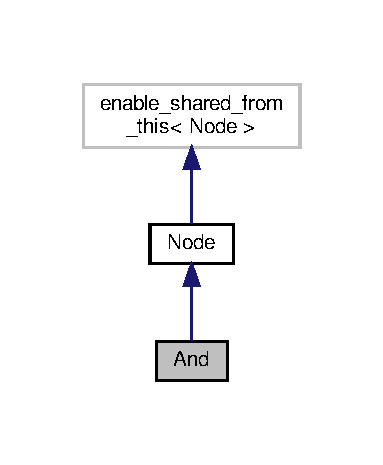
\includegraphics[width=184pt]{dc/d54/class_and__inherit__graph}
\end{center}
\end{figure}


Collaboration diagram for And\+:\nopagebreak
\begin{figure}[H]
\begin{center}
\leavevmode
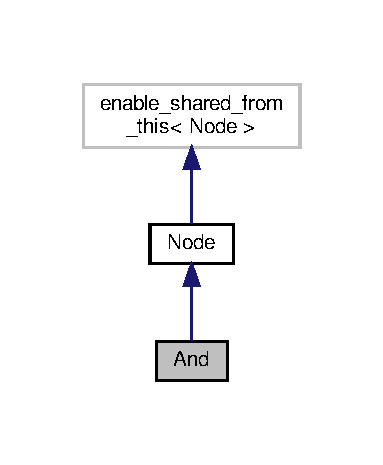
\includegraphics[width=184pt]{d7/d3e/class_and__coll__graph}
\end{center}
\end{figure}
\subsection*{Public Member Functions}
\begin{DoxyCompactItemize}
\item 
\hyperlink{class_and_a6058f4ed6168568b529e1e0750df8cf8}{And} (shared\+\_\+ptr$<$ \hyperlink{class_node}{Node} $>$ l=nullptr, shared\+\_\+ptr$<$ \hyperlink{class_node}{Node} $>$ r=nullptr)
\item 
\hyperlink{class_and_af7bc87f11ac21a32c28c194f3eb94650}{$\sim$\+And} () override
\item 
bool \hyperlink{class_and_a9d2b965d8a1b80d0e2da9d6537601e14}{get\+Value} (string val\+List) override
\begin{DoxyCompactList}\small\item\em get proposition value \end{DoxyCompactList}\item 
\hyperlink{proposition_2tableaux_2enum_8h_a70c93904c6a27d228050f922eb4fc3b8}{R\+U\+L\+ES} \hyperlink{class_and_a9b62ef9a38c6fe9ac96c958d46e30f7b}{get\+S\+T\+Rule\+Name} (bool is\+Negation) override
\begin{DoxyCompactList}\small\item\em get semantic taubleux rule name \end{DoxyCompactList}\item 
shared\+\_\+ptr$<$ \hyperlink{class_node}{Node} $>$ \hyperlink{class_and_a790a8f5b095f664f0a879d2bf96c972d}{nandify} (bool is\+Negation) override
\begin{DoxyCompactList}\small\item\em nandify proposition \end{DoxyCompactList}\item 
void \hyperlink{class_and_a081ebf199fb2388773a19d2c2044e574}{get\+S\+T\+Node\+Child} (shared\+\_\+ptr$<$ \hyperlink{class_s_t_node}{S\+T\+Node} $>$ root, long pos, bool is\+Negation=false) override
\begin{DoxyCompactList}\small\item\em get semantic taubleaux node child (\hyperlink{class_s_t_node_a19ba8bab4660bdeee0e897687b451a8b}{S\+T\+Node.\+left} and \hyperlink{class_s_t_node_a66d06118063fb739058f91c75b725e27}{S\+T\+Node.\+right}) \end{DoxyCompactList}\item 
shared\+\_\+ptr$<$ \hyperlink{class_node}{Node} $>$ \hyperlink{class_and_a18ea23cd682dce93808c34ea0243897f}{cnf\+Filter} (bool is\+Negation=false) override
\begin{DoxyCompactList}\small\item\em in this function node will be \end{DoxyCompactList}\item 
shared\+\_\+ptr$<$ \hyperlink{class_node}{Node} $>$ \hyperlink{class_and_a370c86f44ee17b22208cdbc1f17a7b3f}{cnf\+Distribution} () override
\begin{DoxyCompactList}\small\item\em cnf distribution -\/ this function will be called after set\+Variable \end{DoxyCompactList}\item 
shared\+\_\+ptr$<$ \hyperlink{class_node}{Node} $>$ \hyperlink{class_and_a7560a861ae68050c2aa22e2392a46a15}{copy} () override
\begin{DoxyCompactList}\small\item\em deep copy node \end{DoxyCompactList}\end{DoxyCompactItemize}
\subsection*{Additional Inherited Members}


\subsection{Constructor \& Destructor Documentation}
\mbox{\Hypertarget{class_and_a6058f4ed6168568b529e1e0750df8cf8}\label{class_and_a6058f4ed6168568b529e1e0750df8cf8}} 
\index{And@{And}!And@{And}}
\index{And@{And}!And@{And}}
\subsubsection{\texorpdfstring{And()}{And()}}
{\footnotesize\ttfamily And\+::\+And (\begin{DoxyParamCaption}\item[{shared\+\_\+ptr$<$ \hyperlink{class_node}{Node} $>$}]{l = {\ttfamily nullptr},  }\item[{shared\+\_\+ptr$<$ \hyperlink{class_node}{Node} $>$}]{r = {\ttfamily nullptr} }\end{DoxyParamCaption})\hspace{0.3cm}{\ttfamily [explicit]}}

\mbox{\Hypertarget{class_and_af7bc87f11ac21a32c28c194f3eb94650}\label{class_and_af7bc87f11ac21a32c28c194f3eb94650}} 
\index{And@{And}!````~And@{$\sim$\+And}}
\index{````~And@{$\sim$\+And}!And@{And}}
\subsubsection{\texorpdfstring{$\sim$\+And()}{~And()}}
{\footnotesize\ttfamily And\+::$\sim$\+And (\begin{DoxyParamCaption}{ }\end{DoxyParamCaption})\hspace{0.3cm}{\ttfamily [override]}}



\subsection{Member Function Documentation}
\mbox{\Hypertarget{class_and_a370c86f44ee17b22208cdbc1f17a7b3f}\label{class_and_a370c86f44ee17b22208cdbc1f17a7b3f}} 
\index{And@{And}!cnf\+Distribution@{cnf\+Distribution}}
\index{cnf\+Distribution@{cnf\+Distribution}!And@{And}}
\subsubsection{\texorpdfstring{cnf\+Distribution()}{cnfDistribution()}}
{\footnotesize\ttfamily shared\+\_\+ptr$<$ \hyperlink{class_node}{Node} $>$ And\+::cnf\+Distribution (\begin{DoxyParamCaption}{ }\end{DoxyParamCaption})\hspace{0.3cm}{\ttfamily [override]}, {\ttfamily [virtual]}}



cnf distribution -\/ this function will be called after set\+Variable 

\begin{DoxyReturn}{Returns}
node that applied distribution rule 
\end{DoxyReturn}


Reimplemented from \hyperlink{class_node_ae68e5138f0c1a6c79912e21bc8f39d48}{Node}.

\mbox{\Hypertarget{class_and_a18ea23cd682dce93808c34ea0243897f}\label{class_and_a18ea23cd682dce93808c34ea0243897f}} 
\index{And@{And}!cnf\+Filter@{cnf\+Filter}}
\index{cnf\+Filter@{cnf\+Filter}!And@{And}}
\subsubsection{\texorpdfstring{cnf\+Filter()}{cnfFilter()}}
{\footnotesize\ttfamily shared\+\_\+ptr$<$ \hyperlink{class_node}{Node} $>$ And\+::cnf\+Filter (\begin{DoxyParamCaption}\item[{bool}]{is\+Negation = {\ttfamily false} }\end{DoxyParamCaption})\hspace{0.3cm}{\ttfamily [override]}, {\ttfamily [virtual]}}



in this function node will be 


\begin{DoxyItemize}
\item Remove bi-\/implicate
\item Remove implicate
\item Doing the morgan 
\begin{DoxyParams}{Parameters}
{\em is\+Negation} & -\/ check if this node parent is Negation \\
\hline
\end{DoxyParams}
\begin{DoxyReturn}{Returns}
node has been cnf filtered 
\end{DoxyReturn}

\end{DoxyItemize}

Reimplemented from \hyperlink{class_node_ab5b01fd3c4efe0f2eaf7fc41653359b7}{Node}.

Here is the call graph for this function\+:\nopagebreak
\begin{figure}[H]
\begin{center}
\leavevmode
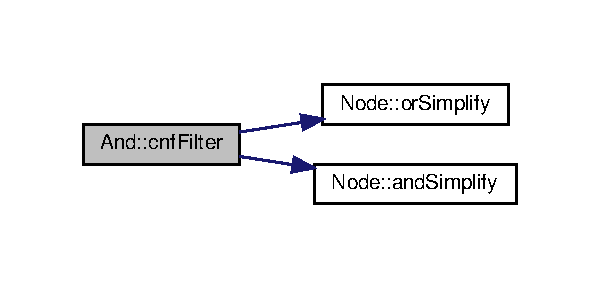
\includegraphics[width=288pt]{d0/dc9/class_and_a18ea23cd682dce93808c34ea0243897f_cgraph}
\end{center}
\end{figure}
\mbox{\Hypertarget{class_and_a7560a861ae68050c2aa22e2392a46a15}\label{class_and_a7560a861ae68050c2aa22e2392a46a15}} 
\index{And@{And}!copy@{copy}}
\index{copy@{copy}!And@{And}}
\subsubsection{\texorpdfstring{copy()}{copy()}}
{\footnotesize\ttfamily shared\+\_\+ptr$<$ \hyperlink{class_node}{Node} $>$ And\+::copy (\begin{DoxyParamCaption}{ }\end{DoxyParamCaption})\hspace{0.3cm}{\ttfamily [override]}, {\ttfamily [virtual]}}



deep copy node 

\begin{DoxyReturn}{Returns}
a deep copy of node 
\end{DoxyReturn}


Reimplemented from \hyperlink{class_node_a0d22a418a622a24852610fd51910c5eb}{Node}.

\mbox{\Hypertarget{class_and_a081ebf199fb2388773a19d2c2044e574}\label{class_and_a081ebf199fb2388773a19d2c2044e574}} 
\index{And@{And}!get\+S\+T\+Node\+Child@{get\+S\+T\+Node\+Child}}
\index{get\+S\+T\+Node\+Child@{get\+S\+T\+Node\+Child}!And@{And}}
\subsubsection{\texorpdfstring{get\+S\+T\+Node\+Child()}{getSTNodeChild()}}
{\footnotesize\ttfamily void And\+::get\+S\+T\+Node\+Child (\begin{DoxyParamCaption}\item[{shared\+\_\+ptr$<$ \hyperlink{class_s_t_node}{S\+T\+Node} $>$}]{root,  }\item[{long}]{pos,  }\item[{bool}]{is\+Negation = {\ttfamily false} }\end{DoxyParamCaption})\hspace{0.3cm}{\ttfamily [override]}, {\ttfamily [virtual]}}



get semantic taubleaux node child (\hyperlink{class_s_t_node_a19ba8bab4660bdeee0e897687b451a8b}{S\+T\+Node.\+left} and \hyperlink{class_s_t_node_a66d06118063fb739058f91c75b725e27}{S\+T\+Node.\+right}) 


\begin{DoxyParams}[1]{Parameters}
\mbox{\tt in}  & {\em root} & -\/ \hyperlink{class_s_t_node}{S\+T\+Node} \\
\hline
\mbox{\tt out}  & {\em root} & -\/ \hyperlink{class_s_t_node}{S\+T\+Node} contains child \\
\hline
 & {\em pos} & -\/ position of child \hyperlink{class_node}{Node} of \hyperlink{class_s_t_node_a370cb3b8a6bcd2e488a27d47be4e0920}{S\+T\+Node\+::nodes} list \\
\hline
 & {\em is\+Negation} & -\/ check if this node parent is Negation \\
\hline
\end{DoxyParams}


Reimplemented from \hyperlink{class_node_a1009cb6d84206c2b5eaa86580da59a7c}{Node}.

\mbox{\Hypertarget{class_and_a9b62ef9a38c6fe9ac96c958d46e30f7b}\label{class_and_a9b62ef9a38c6fe9ac96c958d46e30f7b}} 
\index{And@{And}!get\+S\+T\+Rule\+Name@{get\+S\+T\+Rule\+Name}}
\index{get\+S\+T\+Rule\+Name@{get\+S\+T\+Rule\+Name}!And@{And}}
\subsubsection{\texorpdfstring{get\+S\+T\+Rule\+Name()}{getSTRuleName()}}
{\footnotesize\ttfamily \hyperlink{proposition_2tableaux_2enum_8h_a70c93904c6a27d228050f922eb4fc3b8}{R\+U\+L\+ES} And\+::get\+S\+T\+Rule\+Name (\begin{DoxyParamCaption}\item[{bool}]{is\+Negation }\end{DoxyParamCaption})\hspace{0.3cm}{\ttfamily [override]}, {\ttfamily [virtual]}}



get semantic taubleux rule name 


\begin{DoxyParams}{Parameters}
{\em is\+Negation} & -\/ check if this node parent is Negation \\
\hline
\end{DoxyParams}
\begin{DoxyReturn}{Returns}
R\+U\+L\+ES -\/ semantic taubleaux rule name 
\end{DoxyReturn}


Reimplemented from \hyperlink{class_node_a25b6581950988c2536a392a6874c8072}{Node}.

\mbox{\Hypertarget{class_and_a9d2b965d8a1b80d0e2da9d6537601e14}\label{class_and_a9d2b965d8a1b80d0e2da9d6537601e14}} 
\index{And@{And}!get\+Value@{get\+Value}}
\index{get\+Value@{get\+Value}!And@{And}}
\subsubsection{\texorpdfstring{get\+Value()}{getValue()}}
{\footnotesize\ttfamily bool And\+::get\+Value (\begin{DoxyParamCaption}\item[{string}]{val\+List }\end{DoxyParamCaption})\hspace{0.3cm}{\ttfamily [override]}, {\ttfamily [virtual]}}



get proposition value 


\begin{DoxyParams}{Parameters}
{\em val\+List} & -\/ string contains proposition variable and their value. ~\newline
 e.\+g. \char`\"{}\+A1\+B0\+C1\char`\"{} \\
\hline
\end{DoxyParams}
\begin{DoxyReturn}{Returns}
proposition value 
\end{DoxyReturn}


Reimplemented from \hyperlink{class_node_afd0c2045f3955e02e3aa1e2e987f10b2}{Node}.

\mbox{\Hypertarget{class_and_a790a8f5b095f664f0a879d2bf96c972d}\label{class_and_a790a8f5b095f664f0a879d2bf96c972d}} 
\index{And@{And}!nandify@{nandify}}
\index{nandify@{nandify}!And@{And}}
\subsubsection{\texorpdfstring{nandify()}{nandify()}}
{\footnotesize\ttfamily shared\+\_\+ptr$<$ \hyperlink{class_node}{Node} $>$ And\+::nandify (\begin{DoxyParamCaption}\item[{bool}]{is\+Negation }\end{DoxyParamCaption})\hspace{0.3cm}{\ttfamily [override]}, {\ttfamily [virtual]}}



nandify proposition 


\begin{DoxyParams}{Parameters}
{\em is\+Negation} & -\/ check if this node parent is Negation \\
\hline
\end{DoxyParams}
\begin{DoxyReturn}{Returns}
nandified tree 
\end{DoxyReturn}


Reimplemented from \hyperlink{class_node_a3b2e192b59b7e72908af7903c5a4e5c1}{Node}.



The documentation for this class was generated from the following files\+:\begin{DoxyCompactItemize}
\item 
src/notation/\hyperlink{and_8h}{and.\+h}\item 
src/notation/\hyperlink{and_8cpp}{and.\+cpp}\end{DoxyCompactItemize}

\hypertarget{class_bi_implicate}{}\section{Bi\+Implicate Class Reference}
\label{class_bi_implicate}\index{Bi\+Implicate@{Bi\+Implicate}}


{\ttfamily \#include $<$biimplicate.\+h$>$}



Inheritance diagram for Bi\+Implicate\+:\nopagebreak
\begin{figure}[H]
\begin{center}
\leavevmode
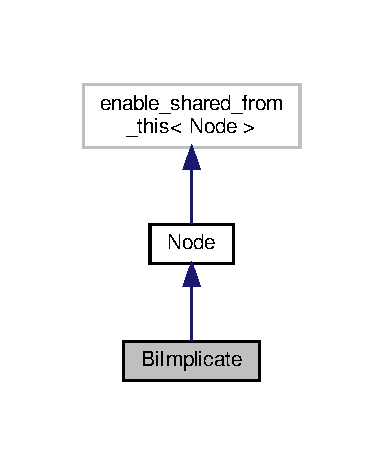
\includegraphics[width=184pt]{da/d01/class_bi_implicate__inherit__graph}
\end{center}
\end{figure}


Collaboration diagram for Bi\+Implicate\+:\nopagebreak
\begin{figure}[H]
\begin{center}
\leavevmode
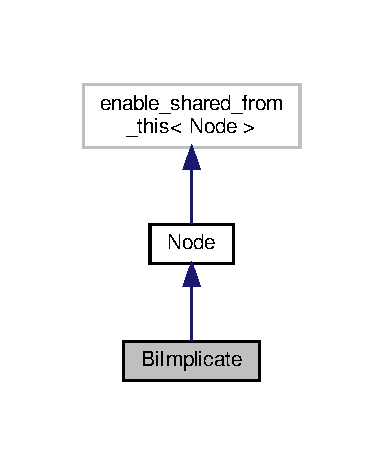
\includegraphics[width=184pt]{d5/d7f/class_bi_implicate__coll__graph}
\end{center}
\end{figure}
\subsection*{Public Member Functions}
\begin{DoxyCompactItemize}
\item 
\hyperlink{class_bi_implicate_acd402fb9b2eef1b44361448038f20ddc}{Bi\+Implicate} (shared\+\_\+ptr$<$ \hyperlink{class_node}{Node} $>$ l=nullptr, shared\+\_\+ptr$<$ \hyperlink{class_node}{Node} $>$ r=nullptr)
\item 
\hyperlink{class_bi_implicate_ad3f12180788d7d207b2e385c2a89c35b}{$\sim$\+Bi\+Implicate} () override
\item 
bool \hyperlink{class_bi_implicate_ac7cb17f1414705f9a1d9df83793b0d58}{get\+Value} (string val\+List) override
\begin{DoxyCompactList}\small\item\em get proposition value \end{DoxyCompactList}\item 
\hyperlink{proposition_2tableaux_2enum_8h_a70c93904c6a27d228050f922eb4fc3b8}{R\+U\+L\+ES} \hyperlink{class_bi_implicate_a3ca1a9b3fd1805b56b72def494179ea3}{get\+S\+T\+Rule\+Name} (bool is\+Negation) override
\begin{DoxyCompactList}\small\item\em get semantic taubleux rule name \end{DoxyCompactList}\item 
shared\+\_\+ptr$<$ \hyperlink{class_node}{Node} $>$ \hyperlink{class_bi_implicate_aa77f25616aa7a47ae4007d661ad60518}{nandify} (bool is\+Negation) override
\begin{DoxyCompactList}\small\item\em nandify proposition \end{DoxyCompactList}\item 
void \hyperlink{class_bi_implicate_a7ecc298b799d533b4bf19b3912932fc7}{get\+S\+T\+Node\+Child} (shared\+\_\+ptr$<$ \hyperlink{class_s_t_node}{S\+T\+Node} $>$ root, long pos, bool is\+Negation) override
\begin{DoxyCompactList}\small\item\em get semantic taubleaux node child (\hyperlink{class_s_t_node_a19ba8bab4660bdeee0e897687b451a8b}{S\+T\+Node.\+left} and \hyperlink{class_s_t_node_a66d06118063fb739058f91c75b725e27}{S\+T\+Node.\+right}) \end{DoxyCompactList}\item 
shared\+\_\+ptr$<$ \hyperlink{class_node}{Node} $>$ \hyperlink{class_bi_implicate_a3f79e7340ff831b0bb927d8a70414ac3}{cnf\+Filter} (bool is\+Negation=false) override
\begin{DoxyCompactList}\small\item\em in this function node will be \end{DoxyCompactList}\item 
shared\+\_\+ptr$<$ \hyperlink{class_node}{Node} $>$ \hyperlink{class_bi_implicate_a41c9d9c53bf05cdde330ec8df07fde31}{copy} () override
\begin{DoxyCompactList}\small\item\em deep copy node \end{DoxyCompactList}\end{DoxyCompactItemize}
\subsection*{Additional Inherited Members}


\subsection{Constructor \& Destructor Documentation}
\mbox{\Hypertarget{class_bi_implicate_acd402fb9b2eef1b44361448038f20ddc}\label{class_bi_implicate_acd402fb9b2eef1b44361448038f20ddc}} 
\index{Bi\+Implicate@{Bi\+Implicate}!Bi\+Implicate@{Bi\+Implicate}}
\index{Bi\+Implicate@{Bi\+Implicate}!Bi\+Implicate@{Bi\+Implicate}}
\subsubsection{\texorpdfstring{Bi\+Implicate()}{BiImplicate()}}
{\footnotesize\ttfamily Bi\+Implicate\+::\+Bi\+Implicate (\begin{DoxyParamCaption}\item[{shared\+\_\+ptr$<$ \hyperlink{class_node}{Node} $>$}]{l = {\ttfamily nullptr},  }\item[{shared\+\_\+ptr$<$ \hyperlink{class_node}{Node} $>$}]{r = {\ttfamily nullptr} }\end{DoxyParamCaption})\hspace{0.3cm}{\ttfamily [explicit]}}

\mbox{\Hypertarget{class_bi_implicate_ad3f12180788d7d207b2e385c2a89c35b}\label{class_bi_implicate_ad3f12180788d7d207b2e385c2a89c35b}} 
\index{Bi\+Implicate@{Bi\+Implicate}!````~Bi\+Implicate@{$\sim$\+Bi\+Implicate}}
\index{````~Bi\+Implicate@{$\sim$\+Bi\+Implicate}!Bi\+Implicate@{Bi\+Implicate}}
\subsubsection{\texorpdfstring{$\sim$\+Bi\+Implicate()}{~BiImplicate()}}
{\footnotesize\ttfamily Bi\+Implicate\+::$\sim$\+Bi\+Implicate (\begin{DoxyParamCaption}{ }\end{DoxyParamCaption})\hspace{0.3cm}{\ttfamily [override]}}



\subsection{Member Function Documentation}
\mbox{\Hypertarget{class_bi_implicate_a3f79e7340ff831b0bb927d8a70414ac3}\label{class_bi_implicate_a3f79e7340ff831b0bb927d8a70414ac3}} 
\index{Bi\+Implicate@{Bi\+Implicate}!cnf\+Filter@{cnf\+Filter}}
\index{cnf\+Filter@{cnf\+Filter}!Bi\+Implicate@{Bi\+Implicate}}
\subsubsection{\texorpdfstring{cnf\+Filter()}{cnfFilter()}}
{\footnotesize\ttfamily shared\+\_\+ptr$<$ \hyperlink{class_node}{Node} $>$ Bi\+Implicate\+::cnf\+Filter (\begin{DoxyParamCaption}\item[{bool}]{is\+Negation = {\ttfamily false} }\end{DoxyParamCaption})\hspace{0.3cm}{\ttfamily [override]}, {\ttfamily [virtual]}}



in this function node will be 


\begin{DoxyItemize}
\item Remove bi-\/implicate
\item Remove implicate
\item Doing the morgan 
\begin{DoxyParams}{Parameters}
{\em is\+Negation} & -\/ check if this node parent is Negation \\
\hline
\end{DoxyParams}
\begin{DoxyReturn}{Returns}
node has been cnf filtered 
\end{DoxyReturn}

\end{DoxyItemize}

Reimplemented from \hyperlink{class_node_ab5b01fd3c4efe0f2eaf7fc41653359b7}{Node}.

Here is the call graph for this function\+:\nopagebreak
\begin{figure}[H]
\begin{center}
\leavevmode
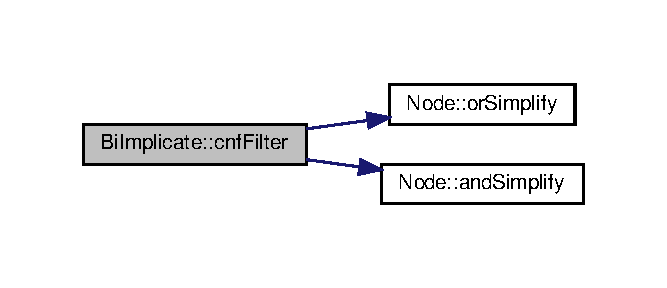
\includegraphics[width=320pt]{d5/da3/class_bi_implicate_a3f79e7340ff831b0bb927d8a70414ac3_cgraph}
\end{center}
\end{figure}
\mbox{\Hypertarget{class_bi_implicate_a41c9d9c53bf05cdde330ec8df07fde31}\label{class_bi_implicate_a41c9d9c53bf05cdde330ec8df07fde31}} 
\index{Bi\+Implicate@{Bi\+Implicate}!copy@{copy}}
\index{copy@{copy}!Bi\+Implicate@{Bi\+Implicate}}
\subsubsection{\texorpdfstring{copy()}{copy()}}
{\footnotesize\ttfamily shared\+\_\+ptr$<$ \hyperlink{class_node}{Node} $>$ Bi\+Implicate\+::copy (\begin{DoxyParamCaption}{ }\end{DoxyParamCaption})\hspace{0.3cm}{\ttfamily [override]}, {\ttfamily [virtual]}}



deep copy node 

\begin{DoxyReturn}{Returns}
a deep copy of node 
\end{DoxyReturn}


Reimplemented from \hyperlink{class_node_a0d22a418a622a24852610fd51910c5eb}{Node}.

\mbox{\Hypertarget{class_bi_implicate_a7ecc298b799d533b4bf19b3912932fc7}\label{class_bi_implicate_a7ecc298b799d533b4bf19b3912932fc7}} 
\index{Bi\+Implicate@{Bi\+Implicate}!get\+S\+T\+Node\+Child@{get\+S\+T\+Node\+Child}}
\index{get\+S\+T\+Node\+Child@{get\+S\+T\+Node\+Child}!Bi\+Implicate@{Bi\+Implicate}}
\subsubsection{\texorpdfstring{get\+S\+T\+Node\+Child()}{getSTNodeChild()}}
{\footnotesize\ttfamily void Bi\+Implicate\+::get\+S\+T\+Node\+Child (\begin{DoxyParamCaption}\item[{shared\+\_\+ptr$<$ \hyperlink{class_s_t_node}{S\+T\+Node} $>$}]{root,  }\item[{long}]{pos,  }\item[{bool}]{is\+Negation }\end{DoxyParamCaption})\hspace{0.3cm}{\ttfamily [override]}, {\ttfamily [virtual]}}



get semantic taubleaux node child (\hyperlink{class_s_t_node_a19ba8bab4660bdeee0e897687b451a8b}{S\+T\+Node.\+left} and \hyperlink{class_s_t_node_a66d06118063fb739058f91c75b725e27}{S\+T\+Node.\+right}) 


\begin{DoxyParams}[1]{Parameters}
\mbox{\tt in}  & {\em root} & -\/ \hyperlink{class_s_t_node}{S\+T\+Node} \\
\hline
\mbox{\tt out}  & {\em root} & -\/ \hyperlink{class_s_t_node}{S\+T\+Node} contains child \\
\hline
 & {\em pos} & -\/ position of child \hyperlink{class_node}{Node} of \hyperlink{class_s_t_node_a370cb3b8a6bcd2e488a27d47be4e0920}{S\+T\+Node\+::nodes} list \\
\hline
 & {\em is\+Negation} & -\/ check if this node parent is Negation \\
\hline
\end{DoxyParams}


Reimplemented from \hyperlink{class_node_a1009cb6d84206c2b5eaa86580da59a7c}{Node}.

\mbox{\Hypertarget{class_bi_implicate_a3ca1a9b3fd1805b56b72def494179ea3}\label{class_bi_implicate_a3ca1a9b3fd1805b56b72def494179ea3}} 
\index{Bi\+Implicate@{Bi\+Implicate}!get\+S\+T\+Rule\+Name@{get\+S\+T\+Rule\+Name}}
\index{get\+S\+T\+Rule\+Name@{get\+S\+T\+Rule\+Name}!Bi\+Implicate@{Bi\+Implicate}}
\subsubsection{\texorpdfstring{get\+S\+T\+Rule\+Name()}{getSTRuleName()}}
{\footnotesize\ttfamily \hyperlink{proposition_2tableaux_2enum_8h_a70c93904c6a27d228050f922eb4fc3b8}{R\+U\+L\+ES} Bi\+Implicate\+::get\+S\+T\+Rule\+Name (\begin{DoxyParamCaption}\item[{bool}]{is\+Negation }\end{DoxyParamCaption})\hspace{0.3cm}{\ttfamily [override]}, {\ttfamily [virtual]}}



get semantic taubleux rule name 


\begin{DoxyParams}{Parameters}
{\em is\+Negation} & -\/ check if this node parent is Negation \\
\hline
\end{DoxyParams}
\begin{DoxyReturn}{Returns}
R\+U\+L\+ES -\/ semantic taubleaux rule name 
\end{DoxyReturn}


Reimplemented from \hyperlink{class_node_a25b6581950988c2536a392a6874c8072}{Node}.

\mbox{\Hypertarget{class_bi_implicate_ac7cb17f1414705f9a1d9df83793b0d58}\label{class_bi_implicate_ac7cb17f1414705f9a1d9df83793b0d58}} 
\index{Bi\+Implicate@{Bi\+Implicate}!get\+Value@{get\+Value}}
\index{get\+Value@{get\+Value}!Bi\+Implicate@{Bi\+Implicate}}
\subsubsection{\texorpdfstring{get\+Value()}{getValue()}}
{\footnotesize\ttfamily bool Bi\+Implicate\+::get\+Value (\begin{DoxyParamCaption}\item[{string}]{val\+List }\end{DoxyParamCaption})\hspace{0.3cm}{\ttfamily [override]}, {\ttfamily [virtual]}}



get proposition value 


\begin{DoxyParams}{Parameters}
{\em val\+List} & -\/ string contains proposition variable and their value. ~\newline
 e.\+g. \char`\"{}\+A1\+B0\+C1\char`\"{} \\
\hline
\end{DoxyParams}
\begin{DoxyReturn}{Returns}
proposition value 
\end{DoxyReturn}


Reimplemented from \hyperlink{class_node_afd0c2045f3955e02e3aa1e2e987f10b2}{Node}.

\mbox{\Hypertarget{class_bi_implicate_aa77f25616aa7a47ae4007d661ad60518}\label{class_bi_implicate_aa77f25616aa7a47ae4007d661ad60518}} 
\index{Bi\+Implicate@{Bi\+Implicate}!nandify@{nandify}}
\index{nandify@{nandify}!Bi\+Implicate@{Bi\+Implicate}}
\subsubsection{\texorpdfstring{nandify()}{nandify()}}
{\footnotesize\ttfamily shared\+\_\+ptr$<$ \hyperlink{class_node}{Node} $>$ Bi\+Implicate\+::nandify (\begin{DoxyParamCaption}\item[{bool}]{is\+Negation }\end{DoxyParamCaption})\hspace{0.3cm}{\ttfamily [override]}, {\ttfamily [virtual]}}



nandify proposition 


\begin{DoxyParams}{Parameters}
{\em is\+Negation} & -\/ check if this node parent is Negation \\
\hline
\end{DoxyParams}
\begin{DoxyReturn}{Returns}
nandified tree 
\end{DoxyReturn}


Reimplemented from \hyperlink{class_node_a3b2e192b59b7e72908af7903c5a4e5c1}{Node}.



The documentation for this class was generated from the following files\+:\begin{DoxyCompactItemize}
\item 
src/notation/\hyperlink{biimplicate_8h}{biimplicate.\+h}\item 
src/notation/\hyperlink{biimplicate_8cpp}{biimplicate.\+cpp}\end{DoxyCompactItemize}

\hypertarget{class_c_n_f}{}\section{C\+NF Class Reference}
\label{class_c_n_f}\index{C\+NF@{C\+NF}}


The \hyperlink{class_c_n_f}{C\+NF} class.  




{\ttfamily \#include $<$cnf.\+h$>$}



Inheritance diagram for C\+NF\+:\nopagebreak
\begin{figure}[H]
\begin{center}
\leavevmode
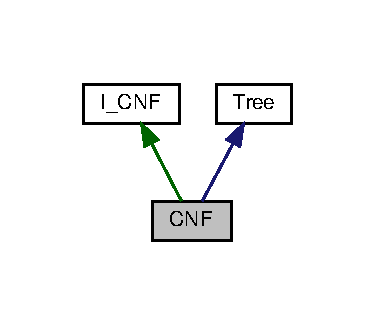
\includegraphics[width=180pt]{d2/d91/class_c_n_f__inherit__graph}
\end{center}
\end{figure}


Collaboration diagram for C\+NF\+:\nopagebreak
\begin{figure}[H]
\begin{center}
\leavevmode
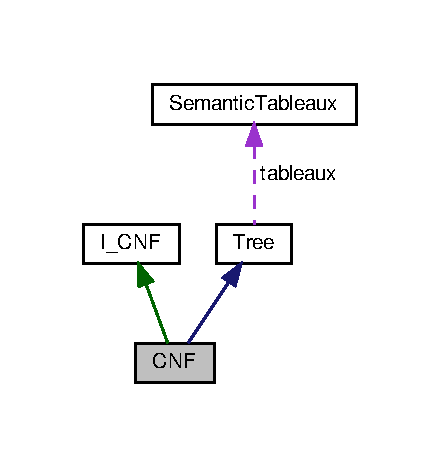
\includegraphics[width=211pt]{d3/d9e/class_c_n_f__coll__graph}
\end{center}
\end{figure}
\subsection*{Public Member Functions}
\begin{DoxyCompactItemize}
\item 
\hyperlink{class_c_n_f_af775e3be36e475027355d21e9ba43166}{C\+NF} (shared\+\_\+ptr$<$ \hyperlink{class_node}{Node} $>$ other\+Tree)
\begin{DoxyCompactList}\small\item\em \hyperlink{class_c_n_f}{C\+NF} constructor, generate \hyperlink{class_c_n_f}{C\+NF} of normal tree. \end{DoxyCompactList}\item 
\hyperlink{class_c_n_f_acb13869409764d8abbea2e50910fd7bc}{C\+NF} (string prop=\char`\"{}\char`\"{})
\begin{DoxyCompactList}\small\item\em \hyperlink{class_c_n_f}{C\+NF} constructor, parse a \hyperlink{class_c_n_f}{C\+NF} tree. \end{DoxyCompactList}\item 
\hyperlink{class_c_n_f_a7bce39709f41a431d486f988b32646de}{$\sim$\+C\+NF} () override
\item 
string \hyperlink{class_c_n_f_a029535415f1d5cf92c8023693ce7b40e}{get\+David\+Putnam} () override
\begin{DoxyCompactList}\small\item\em get David Putnam \end{DoxyCompactList}\item 
list$<$ string $>$ \hyperlink{class_c_n_f_abb762bfe4bc7bbccda81f8db332bafe3}{get\+List\+Variable} () override
\end{DoxyCompactItemize}
\subsection*{Private Member Functions}
\begin{DoxyCompactItemize}
\item 
shared\+\_\+ptr$<$ \hyperlink{class_node}{Node} $>$ \hyperlink{class_c_n_f_a5232071e600e1bfbb76ad7d0e10d7d92}{parse} (string prop)
\begin{DoxyCompactList}\small\item\em parse cnf proposition \end{DoxyCompactList}\item 
shared\+\_\+ptr$<$ \hyperlink{class_node}{Node} $>$ \hyperlink{class_c_n_f_af2c396e921388daa2e99b6fef25b6697}{get\+Multi\+Or} (string prop)
\begin{DoxyCompactList}\small\item\em get \hyperlink{class_multi_or}{Multi\+Or} base on proposition \end{DoxyCompactList}\item 
void \hyperlink{class_c_n_f_a0ae7d61f4d57fca35ff619af3300e63c}{get\+David\+Putnam} (shared\+\_\+ptr$<$ \hyperlink{class_node}{Node} $>$ \hyperlink{class_tree_a9c0875a8767528453814b8e3daf8f9af}{tree}, uint pos, string \&result)
\begin{DoxyCompactList}\small\item\em get David Putnam, this function is used by a public function \end{DoxyCompactList}\end{DoxyCompactItemize}
\subsection*{Additional Inherited Members}


\subsection{Detailed Description}
The \hyperlink{class_c_n_f}{C\+NF} class. 

\subsection{Constructor \& Destructor Documentation}
\mbox{\Hypertarget{class_c_n_f_af775e3be36e475027355d21e9ba43166}\label{class_c_n_f_af775e3be36e475027355d21e9ba43166}} 
\index{C\+NF@{C\+NF}!C\+NF@{C\+NF}}
\index{C\+NF@{C\+NF}!C\+NF@{C\+NF}}
\subsubsection{\texorpdfstring{C\+N\+F()}{CNF()}\hspace{0.1cm}{\footnotesize\ttfamily [1/2]}}
{\footnotesize\ttfamily C\+N\+F\+::\+C\+NF (\begin{DoxyParamCaption}\item[{shared\+\_\+ptr$<$ \hyperlink{class_node}{Node} $>$}]{other\+Tree }\end{DoxyParamCaption})}



\hyperlink{class_c_n_f}{C\+NF} constructor, generate \hyperlink{class_c_n_f}{C\+NF} of normal tree. 


\begin{DoxyParams}{Parameters}
{\em other\+Tree} & -\/ tree to be convert to cnf form \\
\hline
\end{DoxyParams}
Here is the call graph for this function\+:\nopagebreak
\begin{figure}[H]
\begin{center}
\leavevmode
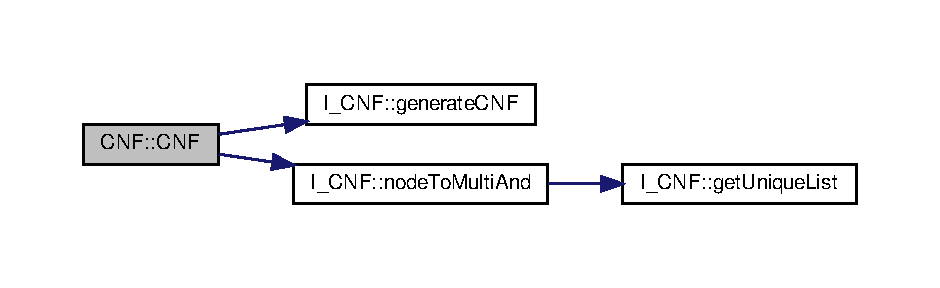
\includegraphics[width=350pt]{dc/d0e/class_c_n_f_af775e3be36e475027355d21e9ba43166_cgraph}
\end{center}
\end{figure}
\mbox{\Hypertarget{class_c_n_f_acb13869409764d8abbea2e50910fd7bc}\label{class_c_n_f_acb13869409764d8abbea2e50910fd7bc}} 
\index{C\+NF@{C\+NF}!C\+NF@{C\+NF}}
\index{C\+NF@{C\+NF}!C\+NF@{C\+NF}}
\subsubsection{\texorpdfstring{C\+N\+F()}{CNF()}\hspace{0.1cm}{\footnotesize\ttfamily [2/2]}}
{\footnotesize\ttfamily C\+N\+F\+::\+C\+NF (\begin{DoxyParamCaption}\item[{string}]{prop = {\ttfamily \char`\"{}\char`\"{}} }\end{DoxyParamCaption})}



\hyperlink{class_c_n_f}{C\+NF} constructor, parse a \hyperlink{class_c_n_f}{C\+NF} tree. 


\begin{DoxyParams}{Parameters}
{\em prop} & -\/ proposition \\
\hline
\end{DoxyParams}
Here is the call graph for this function\+:\nopagebreak
\begin{figure}[H]
\begin{center}
\leavevmode
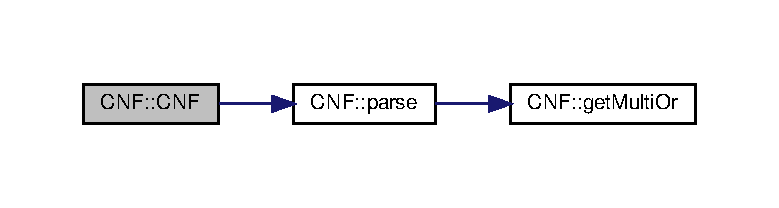
\includegraphics[width=350pt]{dc/d0e/class_c_n_f_acb13869409764d8abbea2e50910fd7bc_cgraph}
\end{center}
\end{figure}
\mbox{\Hypertarget{class_c_n_f_a7bce39709f41a431d486f988b32646de}\label{class_c_n_f_a7bce39709f41a431d486f988b32646de}} 
\index{C\+NF@{C\+NF}!````~C\+NF@{$\sim$\+C\+NF}}
\index{````~C\+NF@{$\sim$\+C\+NF}!C\+NF@{C\+NF}}
\subsubsection{\texorpdfstring{$\sim$\+C\+N\+F()}{~CNF()}}
{\footnotesize\ttfamily C\+N\+F\+::$\sim$\+C\+NF (\begin{DoxyParamCaption}{ }\end{DoxyParamCaption})\hspace{0.3cm}{\ttfamily [override]}}



\subsection{Member Function Documentation}
\mbox{\Hypertarget{class_c_n_f_a029535415f1d5cf92c8023693ce7b40e}\label{class_c_n_f_a029535415f1d5cf92c8023693ce7b40e}} 
\index{C\+NF@{C\+NF}!get\+David\+Putnam@{get\+David\+Putnam}}
\index{get\+David\+Putnam@{get\+David\+Putnam}!C\+NF@{C\+NF}}
\subsubsection{\texorpdfstring{get\+David\+Putnam()}{getDavidPutnam()}\hspace{0.1cm}{\footnotesize\ttfamily [1/2]}}
{\footnotesize\ttfamily string C\+N\+F\+::get\+David\+Putnam (\begin{DoxyParamCaption}{ }\end{DoxyParamCaption})\hspace{0.3cm}{\ttfamily [override]}, {\ttfamily [virtual]}}



get David Putnam 

\begin{DoxyReturn}{Returns}
string, showing David Putnam result 
\end{DoxyReturn}


Reimplemented from \hyperlink{class_tree_a9d7b51cc207222de02ccb59192454de5}{Tree}.

Here is the call graph for this function\+:\nopagebreak
\begin{figure}[H]
\begin{center}
\leavevmode
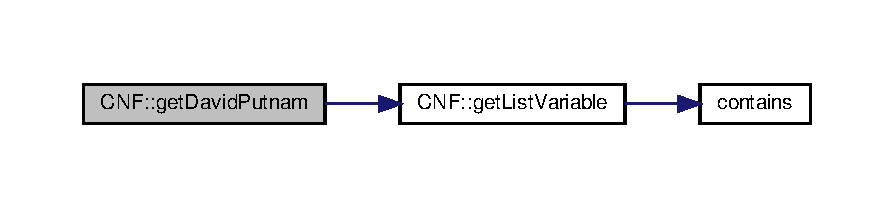
\includegraphics[width=350pt]{dc/d0e/class_c_n_f_a029535415f1d5cf92c8023693ce7b40e_cgraph}
\end{center}
\end{figure}
Here is the caller graph for this function\+:\nopagebreak
\begin{figure}[H]
\begin{center}
\leavevmode
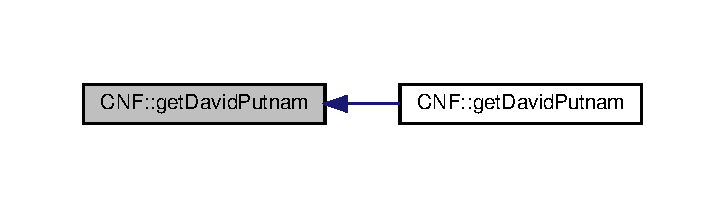
\includegraphics[width=348pt]{dc/d0e/class_c_n_f_a029535415f1d5cf92c8023693ce7b40e_icgraph}
\end{center}
\end{figure}
\mbox{\Hypertarget{class_c_n_f_a0ae7d61f4d57fca35ff619af3300e63c}\label{class_c_n_f_a0ae7d61f4d57fca35ff619af3300e63c}} 
\index{C\+NF@{C\+NF}!get\+David\+Putnam@{get\+David\+Putnam}}
\index{get\+David\+Putnam@{get\+David\+Putnam}!C\+NF@{C\+NF}}
\subsubsection{\texorpdfstring{get\+David\+Putnam()}{getDavidPutnam()}\hspace{0.1cm}{\footnotesize\ttfamily [2/2]}}
{\footnotesize\ttfamily void C\+N\+F\+::get\+David\+Putnam (\begin{DoxyParamCaption}\item[{shared\+\_\+ptr$<$ \hyperlink{class_node}{Node} $>$}]{tree,  }\item[{uint}]{pos,  }\item[{string \&}]{result }\end{DoxyParamCaption})\hspace{0.3cm}{\ttfamily [private]}}



get David Putnam, this function is used by a public function 


\begin{DoxyParams}[1]{Parameters}
 & {\em tree} & -\/ cnf tree \\
\hline
 & {\em pos} & -\/ current variable position \\
\hline
\mbox{\tt out}  & {\em result} & -\/ string, represent Devaid Putname result \\
\hline
\end{DoxyParams}
Here is the call graph for this function\+:\nopagebreak
\begin{figure}[H]
\begin{center}
\leavevmode
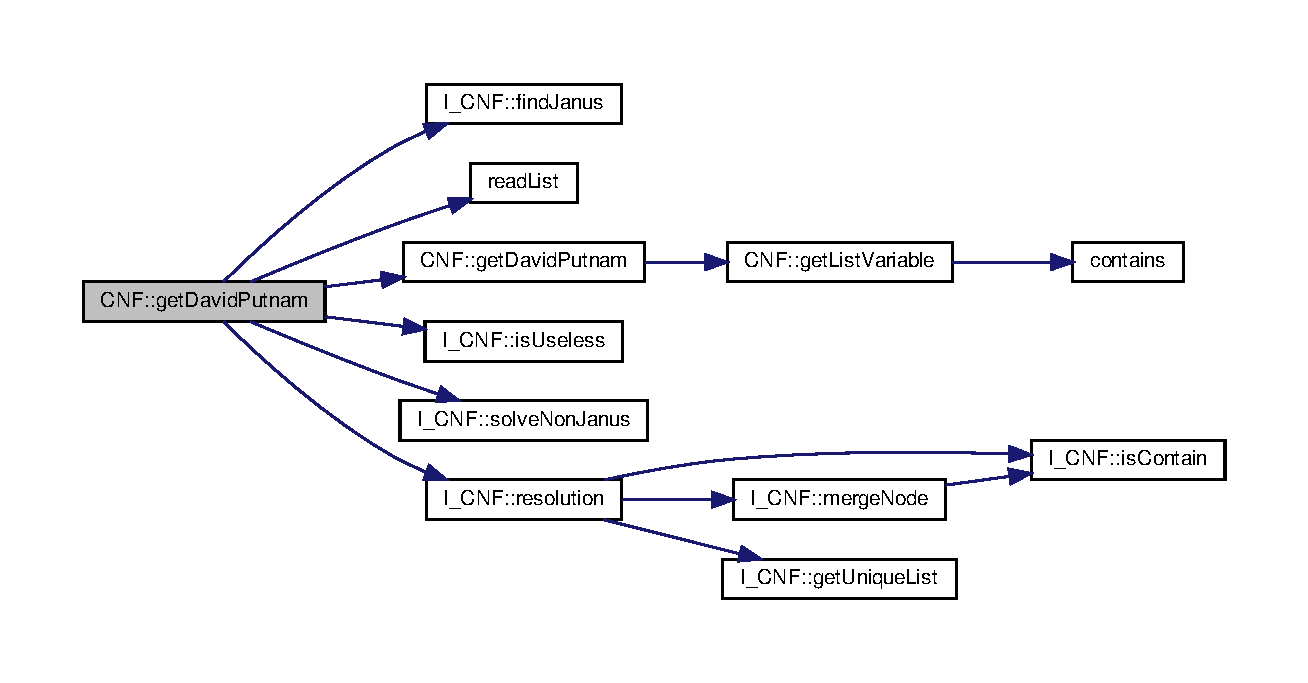
\includegraphics[width=350pt]{dc/d0e/class_c_n_f_a0ae7d61f4d57fca35ff619af3300e63c_cgraph}
\end{center}
\end{figure}
\mbox{\Hypertarget{class_c_n_f_abb762bfe4bc7bbccda81f8db332bafe3}\label{class_c_n_f_abb762bfe4bc7bbccda81f8db332bafe3}} 
\index{C\+NF@{C\+NF}!get\+List\+Variable@{get\+List\+Variable}}
\index{get\+List\+Variable@{get\+List\+Variable}!C\+NF@{C\+NF}}
\subsubsection{\texorpdfstring{get\+List\+Variable()}{getListVariable()}}
{\footnotesize\ttfamily list$<$ string $>$ C\+N\+F\+::get\+List\+Variable (\begin{DoxyParamCaption}{ }\end{DoxyParamCaption})\hspace{0.3cm}{\ttfamily [override]}, {\ttfamily [virtual]}}



Reimplemented from \hyperlink{class_tree_a525967d14a17de0ad9c9072b025af1c3}{Tree}.

Here is the call graph for this function\+:\nopagebreak
\begin{figure}[H]
\begin{center}
\leavevmode
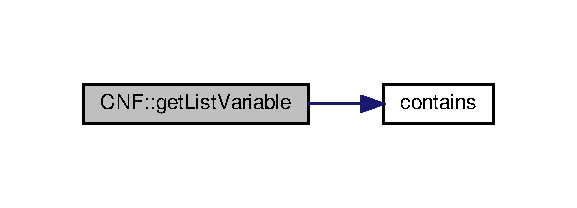
\includegraphics[width=277pt]{dc/d0e/class_c_n_f_abb762bfe4bc7bbccda81f8db332bafe3_cgraph}
\end{center}
\end{figure}
Here is the caller graph for this function\+:\nopagebreak
\begin{figure}[H]
\begin{center}
\leavevmode
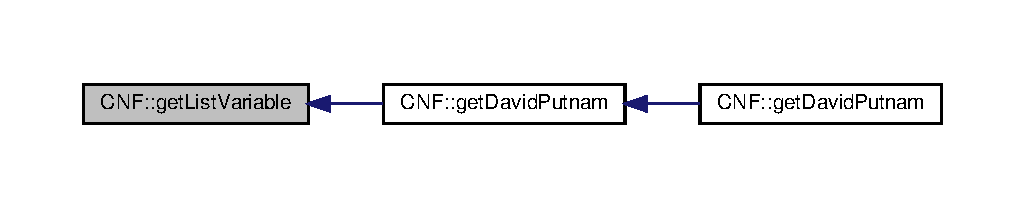
\includegraphics[width=350pt]{dc/d0e/class_c_n_f_abb762bfe4bc7bbccda81f8db332bafe3_icgraph}
\end{center}
\end{figure}
\mbox{\Hypertarget{class_c_n_f_af2c396e921388daa2e99b6fef25b6697}\label{class_c_n_f_af2c396e921388daa2e99b6fef25b6697}} 
\index{C\+NF@{C\+NF}!get\+Multi\+Or@{get\+Multi\+Or}}
\index{get\+Multi\+Or@{get\+Multi\+Or}!C\+NF@{C\+NF}}
\subsubsection{\texorpdfstring{get\+Multi\+Or()}{getMultiOr()}}
{\footnotesize\ttfamily shared\+\_\+ptr$<$ \hyperlink{class_node}{Node} $>$ C\+N\+F\+::get\+Multi\+Or (\begin{DoxyParamCaption}\item[{string}]{prop }\end{DoxyParamCaption})\hspace{0.3cm}{\ttfamily [private]}}



get \hyperlink{class_multi_or}{Multi\+Or} base on proposition 


\begin{DoxyParams}{Parameters}
{\em prop} & -\/ cnf string of proposition \\
\hline
\end{DoxyParams}
\begin{DoxyReturn}{Returns}
\hyperlink{class_multi_or}{Multi\+Or} represent proposition 
\end{DoxyReturn}
Here is the caller graph for this function\+:\nopagebreak
\begin{figure}[H]
\begin{center}
\leavevmode
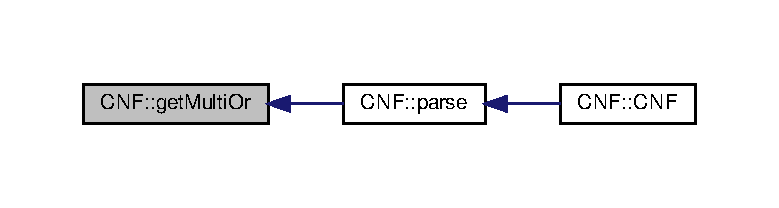
\includegraphics[width=350pt]{dc/d0e/class_c_n_f_af2c396e921388daa2e99b6fef25b6697_icgraph}
\end{center}
\end{figure}
\mbox{\Hypertarget{class_c_n_f_a5232071e600e1bfbb76ad7d0e10d7d92}\label{class_c_n_f_a5232071e600e1bfbb76ad7d0e10d7d92}} 
\index{C\+NF@{C\+NF}!parse@{parse}}
\index{parse@{parse}!C\+NF@{C\+NF}}
\subsubsection{\texorpdfstring{parse()}{parse()}}
{\footnotesize\ttfamily shared\+\_\+ptr$<$ \hyperlink{class_node}{Node} $>$ C\+N\+F\+::parse (\begin{DoxyParamCaption}\item[{string}]{prop }\end{DoxyParamCaption})\hspace{0.3cm}{\ttfamily [private]}}



parse cnf proposition 


\begin{DoxyParams}{Parameters}
{\em prop} & -\/ cnf string of proposition \\
\hline
\end{DoxyParams}
\begin{DoxyReturn}{Returns}
\hyperlink{class_multi_and}{Multi\+And} represent proposition 
\end{DoxyReturn}
Here is the call graph for this function\+:\nopagebreak
\begin{figure}[H]
\begin{center}
\leavevmode
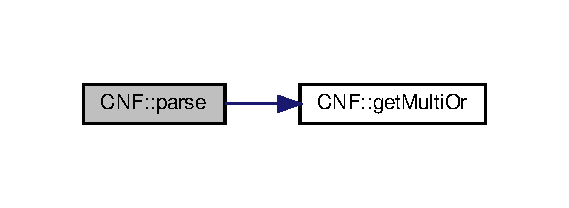
\includegraphics[width=273pt]{dc/d0e/class_c_n_f_a5232071e600e1bfbb76ad7d0e10d7d92_cgraph}
\end{center}
\end{figure}
Here is the caller graph for this function\+:\nopagebreak
\begin{figure}[H]
\begin{center}
\leavevmode
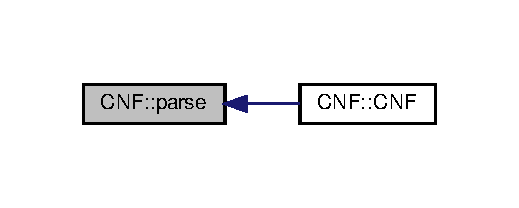
\includegraphics[width=249pt]{dc/d0e/class_c_n_f_a5232071e600e1bfbb76ad7d0e10d7d92_icgraph}
\end{center}
\end{figure}


The documentation for this class was generated from the following files\+:\begin{DoxyCompactItemize}
\item 
src/cnf/\hyperlink{cnf_8h}{cnf.\+h}\item 
src/cnf/\hyperlink{cnf_8cpp}{cnf.\+cpp}\end{DoxyCompactItemize}

\hypertarget{class_exists}{}\section{Exists Class Reference}
\label{class_exists}\index{Exists@{Exists}}


{\ttfamily \#include $<$exists.\+h$>$}



Inheritance diagram for Exists\+:\nopagebreak
\begin{figure}[H]
\begin{center}
\leavevmode
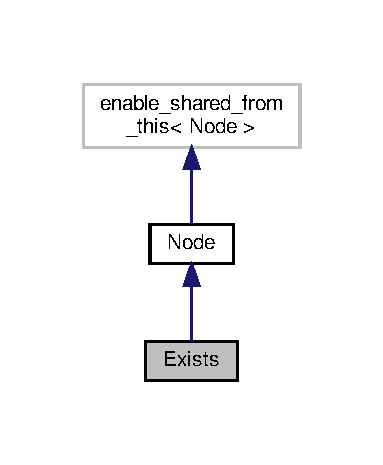
\includegraphics[width=184pt]{d0/d4c/class_exists__inherit__graph}
\end{center}
\end{figure}


Collaboration diagram for Exists\+:\nopagebreak
\begin{figure}[H]
\begin{center}
\leavevmode
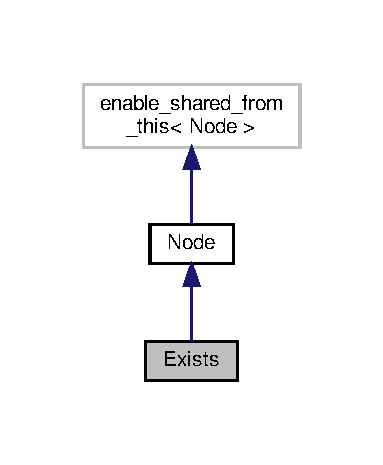
\includegraphics[width=184pt]{d2/d90/class_exists__coll__graph}
\end{center}
\end{figure}
\subsection*{Public Member Functions}
\begin{DoxyCompactItemize}
\item 
\hyperlink{class_exists_ae51931aa14079e565a7b700b8f1d1fb1}{Exists} (shared\+\_\+ptr$<$ \hyperlink{class_node}{Node} $>$ l=nullptr, shared\+\_\+ptr$<$ \hyperlink{class_node}{Node} $>$ r=nullptr)
\item 
\hyperlink{class_exists_a12ebe07a95afddca068d6cbdd67508f2}{$\sim$\+Exists} () override
\item 
string \hyperlink{class_exists_a8eda64d4fd60158c15b38f64a4596068}{to\+String} () override
\begin{DoxyCompactList}\small\item\em get proposition infix formular \end{DoxyCompactList}\item 
\hyperlink{proposition_2tableaux_2enum_8h_a70c93904c6a27d228050f922eb4fc3b8}{R\+U\+L\+ES} \hyperlink{class_exists_aff7b8694345884d06bdd751e88fae041}{get\+S\+T\+Rule\+Name} (bool is\+Negation) override
\begin{DoxyCompactList}\small\item\em get semantic taubleux rule name \end{DoxyCompactList}\item 
void \hyperlink{class_exists_ad60177b343503d1ee8bdda801c2d32d6}{get\+S\+T\+Node\+Child} (shared\+\_\+ptr$<$ \hyperlink{class_s_t_node}{S\+T\+Node} $>$ root, long pos, bool is\+Negation) override
\begin{DoxyCompactList}\small\item\em get semantic taubleaux node child (\hyperlink{class_s_t_node_a19ba8bab4660bdeee0e897687b451a8b}{S\+T\+Node.\+left} and \hyperlink{class_s_t_node_a66d06118063fb739058f91c75b725e27}{S\+T\+Node.\+right}) \end{DoxyCompactList}\item 
shared\+\_\+ptr$<$ \hyperlink{class_node}{Node} $>$ \hyperlink{class_exists_a135277d9bfed780d4ea493ef355055d4}{copy} () override
\begin{DoxyCompactList}\small\item\em deep copy node \end{DoxyCompactList}\end{DoxyCompactItemize}
\subsection*{Additional Inherited Members}


\subsection{Constructor \& Destructor Documentation}
\mbox{\Hypertarget{class_exists_ae51931aa14079e565a7b700b8f1d1fb1}\label{class_exists_ae51931aa14079e565a7b700b8f1d1fb1}} 
\index{Exists@{Exists}!Exists@{Exists}}
\index{Exists@{Exists}!Exists@{Exists}}
\subsubsection{\texorpdfstring{Exists()}{Exists()}}
{\footnotesize\ttfamily Exists\+::\+Exists (\begin{DoxyParamCaption}\item[{shared\+\_\+ptr$<$ \hyperlink{class_node}{Node} $>$}]{l = {\ttfamily nullptr},  }\item[{shared\+\_\+ptr$<$ \hyperlink{class_node}{Node} $>$}]{r = {\ttfamily nullptr} }\end{DoxyParamCaption})}

\mbox{\Hypertarget{class_exists_a12ebe07a95afddca068d6cbdd67508f2}\label{class_exists_a12ebe07a95afddca068d6cbdd67508f2}} 
\index{Exists@{Exists}!````~Exists@{$\sim$\+Exists}}
\index{````~Exists@{$\sim$\+Exists}!Exists@{Exists}}
\subsubsection{\texorpdfstring{$\sim$\+Exists()}{~Exists()}}
{\footnotesize\ttfamily Exists\+::$\sim$\+Exists (\begin{DoxyParamCaption}{ }\end{DoxyParamCaption})\hspace{0.3cm}{\ttfamily [override]}}



\subsection{Member Function Documentation}
\mbox{\Hypertarget{class_exists_a135277d9bfed780d4ea493ef355055d4}\label{class_exists_a135277d9bfed780d4ea493ef355055d4}} 
\index{Exists@{Exists}!copy@{copy}}
\index{copy@{copy}!Exists@{Exists}}
\subsubsection{\texorpdfstring{copy()}{copy()}}
{\footnotesize\ttfamily shared\+\_\+ptr$<$ \hyperlink{class_node}{Node} $>$ Exists\+::copy (\begin{DoxyParamCaption}{ }\end{DoxyParamCaption})\hspace{0.3cm}{\ttfamily [override]}, {\ttfamily [virtual]}}



deep copy node 

\begin{DoxyReturn}{Returns}
a deep copy of node 
\end{DoxyReturn}


Reimplemented from \hyperlink{class_node_a0d22a418a622a24852610fd51910c5eb}{Node}.

Here is the caller graph for this function\+:\nopagebreak
\begin{figure}[H]
\begin{center}
\leavevmode
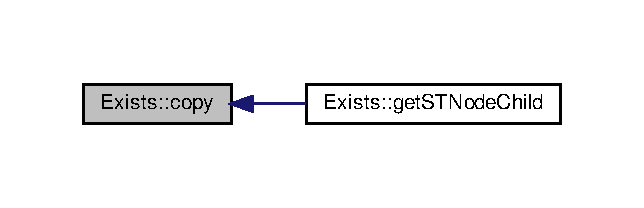
\includegraphics[width=309pt]{de/d16/class_exists_a135277d9bfed780d4ea493ef355055d4_icgraph}
\end{center}
\end{figure}
\mbox{\Hypertarget{class_exists_ad60177b343503d1ee8bdda801c2d32d6}\label{class_exists_ad60177b343503d1ee8bdda801c2d32d6}} 
\index{Exists@{Exists}!get\+S\+T\+Node\+Child@{get\+S\+T\+Node\+Child}}
\index{get\+S\+T\+Node\+Child@{get\+S\+T\+Node\+Child}!Exists@{Exists}}
\subsubsection{\texorpdfstring{get\+S\+T\+Node\+Child()}{getSTNodeChild()}}
{\footnotesize\ttfamily void Exists\+::get\+S\+T\+Node\+Child (\begin{DoxyParamCaption}\item[{shared\+\_\+ptr$<$ \hyperlink{class_s_t_node}{S\+T\+Node} $>$}]{root,  }\item[{long}]{pos,  }\item[{bool}]{is\+Negation }\end{DoxyParamCaption})\hspace{0.3cm}{\ttfamily [override]}, {\ttfamily [virtual]}}



get semantic taubleaux node child (\hyperlink{class_s_t_node_a19ba8bab4660bdeee0e897687b451a8b}{S\+T\+Node.\+left} and \hyperlink{class_s_t_node_a66d06118063fb739058f91c75b725e27}{S\+T\+Node.\+right}) 


\begin{DoxyParams}[1]{Parameters}
\mbox{\tt in}  & {\em root} & -\/ \hyperlink{class_s_t_node}{S\+T\+Node} \\
\hline
\mbox{\tt out}  & {\em root} & -\/ \hyperlink{class_s_t_node}{S\+T\+Node} contains child \\
\hline
 & {\em pos} & -\/ position of child \hyperlink{class_node}{Node} of \hyperlink{class_s_t_node_a370cb3b8a6bcd2e488a27d47be4e0920}{S\+T\+Node\+::nodes} list \\
\hline
 & {\em is\+Negation} & -\/ check if this node parent is Negation \\
\hline
\end{DoxyParams}


Reimplemented from \hyperlink{class_node_a1009cb6d84206c2b5eaa86580da59a7c}{Node}.

Here is the call graph for this function\+:\nopagebreak
\begin{figure}[H]
\begin{center}
\leavevmode
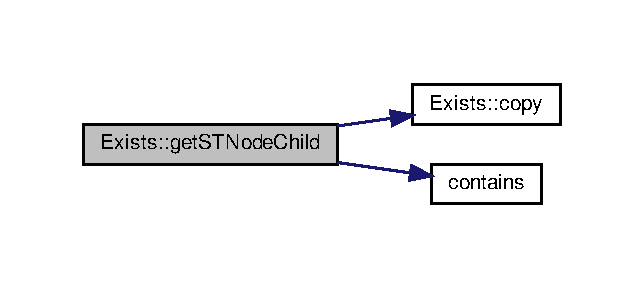
\includegraphics[width=309pt]{de/d16/class_exists_ad60177b343503d1ee8bdda801c2d32d6_cgraph}
\end{center}
\end{figure}
\mbox{\Hypertarget{class_exists_aff7b8694345884d06bdd751e88fae041}\label{class_exists_aff7b8694345884d06bdd751e88fae041}} 
\index{Exists@{Exists}!get\+S\+T\+Rule\+Name@{get\+S\+T\+Rule\+Name}}
\index{get\+S\+T\+Rule\+Name@{get\+S\+T\+Rule\+Name}!Exists@{Exists}}
\subsubsection{\texorpdfstring{get\+S\+T\+Rule\+Name()}{getSTRuleName()}}
{\footnotesize\ttfamily \hyperlink{proposition_2tableaux_2enum_8h_a70c93904c6a27d228050f922eb4fc3b8}{R\+U\+L\+ES} Exists\+::get\+S\+T\+Rule\+Name (\begin{DoxyParamCaption}\item[{bool}]{is\+Negation }\end{DoxyParamCaption})\hspace{0.3cm}{\ttfamily [override]}, {\ttfamily [virtual]}}



get semantic taubleux rule name 


\begin{DoxyParams}{Parameters}
{\em is\+Negation} & -\/ check if this node parent is Negation \\
\hline
\end{DoxyParams}
\begin{DoxyReturn}{Returns}
R\+U\+L\+ES -\/ semantic taubleaux rule name 
\end{DoxyReturn}


Reimplemented from \hyperlink{class_node_a25b6581950988c2536a392a6874c8072}{Node}.

\mbox{\Hypertarget{class_exists_a8eda64d4fd60158c15b38f64a4596068}\label{class_exists_a8eda64d4fd60158c15b38f64a4596068}} 
\index{Exists@{Exists}!to\+String@{to\+String}}
\index{to\+String@{to\+String}!Exists@{Exists}}
\subsubsection{\texorpdfstring{to\+String()}{toString()}}
{\footnotesize\ttfamily string Exists\+::to\+String (\begin{DoxyParamCaption}{ }\end{DoxyParamCaption})\hspace{0.3cm}{\ttfamily [override]}, {\ttfamily [virtual]}}



get proposition infix formular 

\begin{DoxyReturn}{Returns}
string of infix proposition 
\end{DoxyReturn}


Reimplemented from \hyperlink{class_node_a0746502074a232243dcac3b96f3ce2d0}{Node}.



The documentation for this class was generated from the following files\+:\begin{DoxyCompactItemize}
\item 
src/notation/\hyperlink{exists_8h}{exists.\+h}\item 
src/notation/\hyperlink{exists_8cpp}{exists.\+cpp}\end{DoxyCompactItemize}

\hypertarget{class_for_all}{}\section{For\+All Class Reference}
\label{class_for_all}\index{For\+All@{For\+All}}


{\ttfamily \#include $<$forall.\+h$>$}



Inheritance diagram for For\+All\+:\nopagebreak
\begin{figure}[H]
\begin{center}
\leavevmode
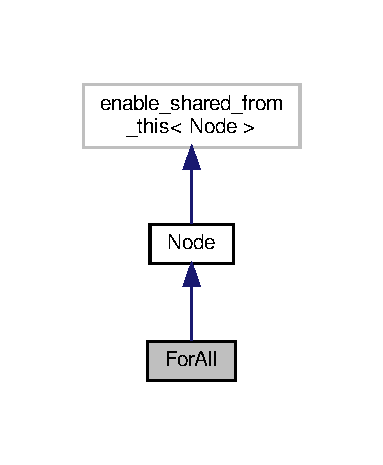
\includegraphics[width=184pt]{d8/d15/class_for_all__inherit__graph}
\end{center}
\end{figure}


Collaboration diagram for For\+All\+:\nopagebreak
\begin{figure}[H]
\begin{center}
\leavevmode
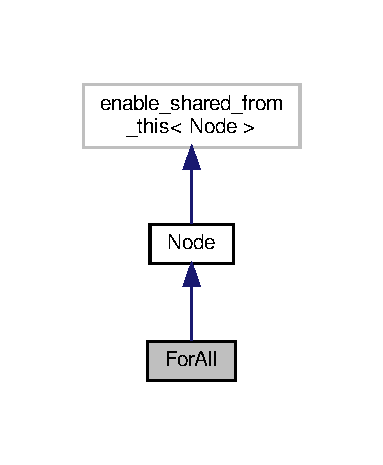
\includegraphics[width=184pt]{df/da8/class_for_all__coll__graph}
\end{center}
\end{figure}
\subsection*{Public Member Functions}
\begin{DoxyCompactItemize}
\item 
\hyperlink{class_for_all_a2f654f00f8d997a89699dff8f1efd759}{For\+All} (shared\+\_\+ptr$<$ \hyperlink{class_node}{Node} $>$ l=nullptr, shared\+\_\+ptr$<$ \hyperlink{class_node}{Node} $>$ r=nullptr)
\item 
\hyperlink{class_for_all_a0c63e42814329a95378fe95f41a369fa}{$\sim$\+For\+All} () override
\item 
string \hyperlink{class_for_all_a086dc15d85fe4874c477c72a40577b85}{to\+String} () override
\begin{DoxyCompactList}\small\item\em get proposition infix formular \end{DoxyCompactList}\item 
\hyperlink{proposition_2tableaux_2enum_8h_a70c93904c6a27d228050f922eb4fc3b8}{R\+U\+L\+ES} \hyperlink{class_for_all_a97e03dcd8f51824fe629487847b7c4dc}{get\+S\+T\+Rule\+Name} (bool is\+Negation) override
\begin{DoxyCompactList}\small\item\em get semantic taubleux rule name \end{DoxyCompactList}\item 
void \hyperlink{class_for_all_a847b6ce62d4e04ce7487b2cc1b49164f}{get\+S\+T\+Node\+Child} (shared\+\_\+ptr$<$ \hyperlink{class_s_t_node}{S\+T\+Node} $>$ root, long pos, bool is\+Negation) override
\begin{DoxyCompactList}\small\item\em get semantic taubleaux node child (\hyperlink{class_s_t_node_a19ba8bab4660bdeee0e897687b451a8b}{S\+T\+Node.\+left} and \hyperlink{class_s_t_node_a66d06118063fb739058f91c75b725e27}{S\+T\+Node.\+right}) \end{DoxyCompactList}\item 
shared\+\_\+ptr$<$ \hyperlink{class_node}{Node} $>$ \hyperlink{class_for_all_ae9b3918a9cd0870a20b80db2288fe402}{copy} () override
\begin{DoxyCompactList}\small\item\em deep copy node \end{DoxyCompactList}\end{DoxyCompactItemize}
\subsection*{Additional Inherited Members}


\subsection{Constructor \& Destructor Documentation}
\mbox{\Hypertarget{class_for_all_a2f654f00f8d997a89699dff8f1efd759}\label{class_for_all_a2f654f00f8d997a89699dff8f1efd759}} 
\index{For\+All@{For\+All}!For\+All@{For\+All}}
\index{For\+All@{For\+All}!For\+All@{For\+All}}
\subsubsection{\texorpdfstring{For\+All()}{ForAll()}}
{\footnotesize\ttfamily For\+All\+::\+For\+All (\begin{DoxyParamCaption}\item[{shared\+\_\+ptr$<$ \hyperlink{class_node}{Node} $>$}]{l = {\ttfamily nullptr},  }\item[{shared\+\_\+ptr$<$ \hyperlink{class_node}{Node} $>$}]{r = {\ttfamily nullptr} }\end{DoxyParamCaption})}

\mbox{\Hypertarget{class_for_all_a0c63e42814329a95378fe95f41a369fa}\label{class_for_all_a0c63e42814329a95378fe95f41a369fa}} 
\index{For\+All@{For\+All}!````~For\+All@{$\sim$\+For\+All}}
\index{````~For\+All@{$\sim$\+For\+All}!For\+All@{For\+All}}
\subsubsection{\texorpdfstring{$\sim$\+For\+All()}{~ForAll()}}
{\footnotesize\ttfamily For\+All\+::$\sim$\+For\+All (\begin{DoxyParamCaption}{ }\end{DoxyParamCaption})\hspace{0.3cm}{\ttfamily [override]}}



\subsection{Member Function Documentation}
\mbox{\Hypertarget{class_for_all_ae9b3918a9cd0870a20b80db2288fe402}\label{class_for_all_ae9b3918a9cd0870a20b80db2288fe402}} 
\index{For\+All@{For\+All}!copy@{copy}}
\index{copy@{copy}!For\+All@{For\+All}}
\subsubsection{\texorpdfstring{copy()}{copy()}}
{\footnotesize\ttfamily shared\+\_\+ptr$<$ \hyperlink{class_node}{Node} $>$ For\+All\+::copy (\begin{DoxyParamCaption}{ }\end{DoxyParamCaption})\hspace{0.3cm}{\ttfamily [override]}, {\ttfamily [virtual]}}



deep copy node 

\begin{DoxyReturn}{Returns}
a deep copy of node 
\end{DoxyReturn}


Reimplemented from \hyperlink{class_node_a0d22a418a622a24852610fd51910c5eb}{Node}.

Here is the caller graph for this function\+:\nopagebreak
\begin{figure}[H]
\begin{center}
\leavevmode
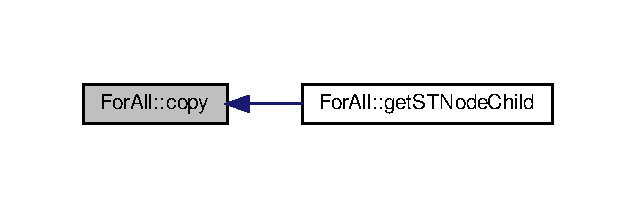
\includegraphics[width=305pt]{d8/dc5/class_for_all_ae9b3918a9cd0870a20b80db2288fe402_icgraph}
\end{center}
\end{figure}
\mbox{\Hypertarget{class_for_all_a847b6ce62d4e04ce7487b2cc1b49164f}\label{class_for_all_a847b6ce62d4e04ce7487b2cc1b49164f}} 
\index{For\+All@{For\+All}!get\+S\+T\+Node\+Child@{get\+S\+T\+Node\+Child}}
\index{get\+S\+T\+Node\+Child@{get\+S\+T\+Node\+Child}!For\+All@{For\+All}}
\subsubsection{\texorpdfstring{get\+S\+T\+Node\+Child()}{getSTNodeChild()}}
{\footnotesize\ttfamily void For\+All\+::get\+S\+T\+Node\+Child (\begin{DoxyParamCaption}\item[{shared\+\_\+ptr$<$ \hyperlink{class_s_t_node}{S\+T\+Node} $>$}]{root,  }\item[{long}]{pos,  }\item[{bool}]{is\+Negation }\end{DoxyParamCaption})\hspace{0.3cm}{\ttfamily [override]}, {\ttfamily [virtual]}}



get semantic taubleaux node child (\hyperlink{class_s_t_node_a19ba8bab4660bdeee0e897687b451a8b}{S\+T\+Node.\+left} and \hyperlink{class_s_t_node_a66d06118063fb739058f91c75b725e27}{S\+T\+Node.\+right}) 


\begin{DoxyParams}[1]{Parameters}
\mbox{\tt in}  & {\em root} & -\/ \hyperlink{class_s_t_node}{S\+T\+Node} \\
\hline
\mbox{\tt out}  & {\em root} & -\/ \hyperlink{class_s_t_node}{S\+T\+Node} contains child \\
\hline
 & {\em pos} & -\/ position of child \hyperlink{class_node}{Node} of \hyperlink{class_s_t_node_a370cb3b8a6bcd2e488a27d47be4e0920}{S\+T\+Node\+::nodes} list \\
\hline
 & {\em is\+Negation} & -\/ check if this node parent is Negation \\
\hline
\end{DoxyParams}


Reimplemented from \hyperlink{class_node_a1009cb6d84206c2b5eaa86580da59a7c}{Node}.

Here is the call graph for this function\+:\nopagebreak
\begin{figure}[H]
\begin{center}
\leavevmode
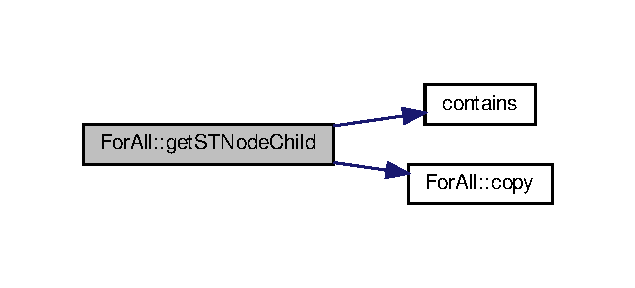
\includegraphics[width=305pt]{d8/dc5/class_for_all_a847b6ce62d4e04ce7487b2cc1b49164f_cgraph}
\end{center}
\end{figure}
\mbox{\Hypertarget{class_for_all_a97e03dcd8f51824fe629487847b7c4dc}\label{class_for_all_a97e03dcd8f51824fe629487847b7c4dc}} 
\index{For\+All@{For\+All}!get\+S\+T\+Rule\+Name@{get\+S\+T\+Rule\+Name}}
\index{get\+S\+T\+Rule\+Name@{get\+S\+T\+Rule\+Name}!For\+All@{For\+All}}
\subsubsection{\texorpdfstring{get\+S\+T\+Rule\+Name()}{getSTRuleName()}}
{\footnotesize\ttfamily \hyperlink{proposition_2tableaux_2enum_8h_a70c93904c6a27d228050f922eb4fc3b8}{R\+U\+L\+ES} For\+All\+::get\+S\+T\+Rule\+Name (\begin{DoxyParamCaption}\item[{bool}]{is\+Negation }\end{DoxyParamCaption})\hspace{0.3cm}{\ttfamily [override]}, {\ttfamily [virtual]}}



get semantic taubleux rule name 


\begin{DoxyParams}{Parameters}
{\em is\+Negation} & -\/ check if this node parent is Negation \\
\hline
\end{DoxyParams}
\begin{DoxyReturn}{Returns}
R\+U\+L\+ES -\/ semantic taubleaux rule name 
\end{DoxyReturn}


Reimplemented from \hyperlink{class_node_a25b6581950988c2536a392a6874c8072}{Node}.

\mbox{\Hypertarget{class_for_all_a086dc15d85fe4874c477c72a40577b85}\label{class_for_all_a086dc15d85fe4874c477c72a40577b85}} 
\index{For\+All@{For\+All}!to\+String@{to\+String}}
\index{to\+String@{to\+String}!For\+All@{For\+All}}
\subsubsection{\texorpdfstring{to\+String()}{toString()}}
{\footnotesize\ttfamily string For\+All\+::to\+String (\begin{DoxyParamCaption}{ }\end{DoxyParamCaption})\hspace{0.3cm}{\ttfamily [override]}, {\ttfamily [virtual]}}



get proposition infix formular 

\begin{DoxyReturn}{Returns}
string of infix proposition 
\end{DoxyReturn}


Reimplemented from \hyperlink{class_node_a0746502074a232243dcac3b96f3ce2d0}{Node}.



The documentation for this class was generated from the following files\+:\begin{DoxyCompactItemize}
\item 
src/notation/\hyperlink{forall_8h}{forall.\+h}\item 
src/notation/\hyperlink{forall_8cpp}{forall.\+cpp}\end{DoxyCompactItemize}

\hypertarget{classhandler}{}\section{handler Class Reference}
\label{classhandler}\index{handler@{handler}}


{\ttfamily \#include $<$logging.\+h$>$}

\subsection*{Public Member Functions}
\begin{DoxyCompactItemize}
\item 
\hyperlink{classhandler_a0f44a69126e692e8bc8690539120be75}{handler} ()
\item 
\hyperlink{classhandler_a251fbf93fdf9eba4335c2d2b2f425f51}{handler} (std\+::string fn)
\item 
virtual \hyperlink{classhandler_a290cc764503dcc061a43c7be655ed512}{$\sim$handler} ()
\item 
void \hyperlink{classhandler_a4d5c893a4bd43354effd040fd5946186}{set\+Stream} (std\+::string fn)
\item 
virtual void \hyperlink{classhandler_ae4a74a6e7ba909279833759b4cab2bcc}{write} (std\+::string msg)
\end{DoxyCompactItemize}
\subsection*{Protected Attributes}
\begin{DoxyCompactItemize}
\item 
std\+::ofstream \hyperlink{classhandler_aea02e85ad5696302680d49a66263a2aa}{ofs}
\end{DoxyCompactItemize}


\subsection{Constructor \& Destructor Documentation}
\mbox{\Hypertarget{classhandler_a0f44a69126e692e8bc8690539120be75}\label{classhandler_a0f44a69126e692e8bc8690539120be75}} 
\index{handler@{handler}!handler@{handler}}
\index{handler@{handler}!handler@{handler}}
\subsubsection{\texorpdfstring{handler()}{handler()}\hspace{0.1cm}{\footnotesize\ttfamily [1/2]}}
{\footnotesize\ttfamily handler\+::handler (\begin{DoxyParamCaption}{ }\end{DoxyParamCaption})\hspace{0.3cm}{\ttfamily [explicit]}}

\mbox{\Hypertarget{classhandler_a251fbf93fdf9eba4335c2d2b2f425f51}\label{classhandler_a251fbf93fdf9eba4335c2d2b2f425f51}} 
\index{handler@{handler}!handler@{handler}}
\index{handler@{handler}!handler@{handler}}
\subsubsection{\texorpdfstring{handler()}{handler()}\hspace{0.1cm}{\footnotesize\ttfamily [2/2]}}
{\footnotesize\ttfamily handler\+::handler (\begin{DoxyParamCaption}\item[{std\+::string}]{fn }\end{DoxyParamCaption})\hspace{0.3cm}{\ttfamily [explicit]}}

\mbox{\Hypertarget{classhandler_a290cc764503dcc061a43c7be655ed512}\label{classhandler_a290cc764503dcc061a43c7be655ed512}} 
\index{handler@{handler}!````~handler@{$\sim$handler}}
\index{````~handler@{$\sim$handler}!handler@{handler}}
\subsubsection{\texorpdfstring{$\sim$handler()}{~handler()}}
{\footnotesize\ttfamily handler\+::$\sim$handler (\begin{DoxyParamCaption}{ }\end{DoxyParamCaption})\hspace{0.3cm}{\ttfamily [virtual]}}



\subsection{Member Function Documentation}
\mbox{\Hypertarget{classhandler_a4d5c893a4bd43354effd040fd5946186}\label{classhandler_a4d5c893a4bd43354effd040fd5946186}} 
\index{handler@{handler}!set\+Stream@{set\+Stream}}
\index{set\+Stream@{set\+Stream}!handler@{handler}}
\subsubsection{\texorpdfstring{set\+Stream()}{setStream()}}
{\footnotesize\ttfamily void handler\+::set\+Stream (\begin{DoxyParamCaption}\item[{std\+::string}]{fn }\end{DoxyParamCaption})}

\mbox{\Hypertarget{classhandler_ae4a74a6e7ba909279833759b4cab2bcc}\label{classhandler_ae4a74a6e7ba909279833759b4cab2bcc}} 
\index{handler@{handler}!write@{write}}
\index{write@{write}!handler@{handler}}
\subsubsection{\texorpdfstring{write()}{write()}}
{\footnotesize\ttfamily void handler\+::write (\begin{DoxyParamCaption}\item[{std\+::string}]{msg }\end{DoxyParamCaption})\hspace{0.3cm}{\ttfamily [virtual]}}

Here is the caller graph for this function\+:\nopagebreak
\begin{figure}[H]
\begin{center}
\leavevmode
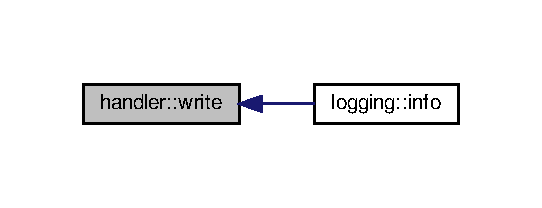
\includegraphics[width=260pt]{d1/df0/classhandler_ae4a74a6e7ba909279833759b4cab2bcc_icgraph}
\end{center}
\end{figure}


\subsection{Member Data Documentation}
\mbox{\Hypertarget{classhandler_aea02e85ad5696302680d49a66263a2aa}\label{classhandler_aea02e85ad5696302680d49a66263a2aa}} 
\index{handler@{handler}!ofs@{ofs}}
\index{ofs@{ofs}!handler@{handler}}
\subsubsection{\texorpdfstring{ofs}{ofs}}
{\footnotesize\ttfamily std\+::ofstream handler\+::ofs\hspace{0.3cm}{\ttfamily [protected]}}



The documentation for this class was generated from the following files\+:\begin{DoxyCompactItemize}
\item 
src/\hyperlink{logging_8h}{logging.\+h}\item 
src/\hyperlink{logging_8cpp}{logging.\+cpp}\end{DoxyCompactItemize}

\hypertarget{struct_i___c_n_f}{}\section{I\+\_\+\+C\+NF Struct Reference}
\label{struct_i___c_n_f}\index{I\+\_\+\+C\+NF@{I\+\_\+\+C\+NF}}


The Public interface of \hyperlink{class_c_n_f}{C\+NF}.  




{\ttfamily \#include $<$cnf.\+h$>$}



Inheritance diagram for I\+\_\+\+C\+NF\+:\nopagebreak
\begin{figure}[H]
\begin{center}
\leavevmode
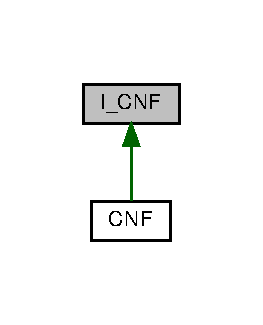
\includegraphics[width=126pt]{da/dda/struct_i___c_n_f__inherit__graph}
\end{center}
\end{figure}
\subsection*{Public Member Functions}
\begin{DoxyCompactItemize}
\item 
string \hyperlink{struct_i___c_n_f_aa7adb25b5dbb1f4dcddaf56dab338add}{solve\+Non\+Janus} (shared\+\_\+ptr$<$ \hyperlink{class_node}{Node} $>$ node, char v)
\begin{DoxyCompactList}\small\item\em Solve non-\/janus based on Muliti\+And node and variable v. \end{DoxyCompactList}\item 
\hyperlink{struct_reso}{Reso} \hyperlink{struct_i___c_n_f_a1b3282ebd2d998f5fe3aa3e192346ac1}{resolution} (shared\+\_\+ptr$<$ \hyperlink{class_node}{Node} $>$ node, char v)
\begin{DoxyCompactList}\small\item\em Resolution based on Muliti\+And node and variable v. \end{DoxyCompactList}\item 
shared\+\_\+ptr$<$ \hyperlink{class_node}{Node} $>$ \hyperlink{struct_i___c_n_f_ac0c5ce2bd3edadb60de923b4259cc10b}{node\+To\+Multi\+And} (shared\+\_\+ptr$<$ \hyperlink{class_node}{Node} $>$ node)
\begin{DoxyCompactList}\small\item\em Convert node to \hyperlink{class_multi_and}{Multi\+And}, remove douplicate element and sort element This function are being used after generate\+C\+NF. \end{DoxyCompactList}\item 
shared\+\_\+ptr$<$ \hyperlink{class_node}{Node} $>$ \hyperlink{struct_i___c_n_f_afedf64bb258fd48ea0f811a9f571f0f0}{generate\+C\+NF} (shared\+\_\+ptr$<$ \hyperlink{class_node}{Node} $>$ origin\+Tree)
\begin{DoxyCompactList}\small\item\em generate \hyperlink{class_c_n_f}{C\+NF} form based on origin\+Tree, origin\+Tree will be changed, to prevent lost data, use deep copy of \hyperlink{class_node}{Node} \end{DoxyCompactList}\end{DoxyCompactItemize}
\subsection*{Static Public Member Functions}
\begin{DoxyCompactItemize}
\item 
static bool \hyperlink{struct_i___c_n_f_ae9f978965edae4ab57c692544cb72d01}{is\+Useless} (shared\+\_\+ptr$<$ \hyperlink{class_node}{Node} $>$ node)
\begin{DoxyCompactList}\small\item\em Check if node is useless. \end{DoxyCompactList}\end{DoxyCompactItemize}
\subsection*{Protected Member Functions}
\begin{DoxyCompactItemize}
\item 
bool \hyperlink{struct_i___c_n_f_ac9fd631eda1871653b2d1fdcd55f18a5}{find\+Janus} (shared\+\_\+ptr$<$ \hyperlink{class_node}{Node} $>$ node)
\begin{DoxyCompactList}\small\item\em Check if \hyperlink{class_node}{Node} contains Janus. \end{DoxyCompactList}\item 
void \hyperlink{struct_i___c_n_f_ad417af0f07b5e7035c3671dcc3e9f798}{get\+Unique\+List} (list$<$ shared\+\_\+ptr$<$ \hyperlink{class_node}{Node} $>$ $>$ \&l)
\begin{DoxyCompactList}\small\item\em get unique list of node \end{DoxyCompactList}\end{DoxyCompactItemize}
\subsection*{Private Member Functions}
\begin{DoxyCompactItemize}
\item 
bool \hyperlink{struct_i___c_n_f_a41a7be439cae3ed577a30b3f2742218e}{is\+Contain} (shared\+\_\+ptr$<$ \hyperlink{class_node}{Node} $>$ nodes, string v)
\begin{DoxyCompactList}\small\item\em check if node contain variable v \end{DoxyCompactList}\item 
shared\+\_\+ptr$<$ \hyperlink{class_node}{Node} $>$ \hyperlink{struct_i___c_n_f_a62586e691ebfb00696be6bf9710f4da4}{merge\+Node} (shared\+\_\+ptr$<$ \hyperlink{class_node}{Node} $>$ node1, shared\+\_\+ptr$<$ \hyperlink{class_node}{Node} $>$ node2, string v, string not\+\_\+v)
\begin{DoxyCompactList}\small\item\em merge two \hyperlink{class_node_a350b631f3a9192bfa23bc266f6b8da02}{Node\+::variables} list. \end{DoxyCompactList}\end{DoxyCompactItemize}


\subsection{Detailed Description}
The Public interface of \hyperlink{class_c_n_f}{C\+NF}. 

\subsection{Member Function Documentation}
\mbox{\Hypertarget{struct_i___c_n_f_ac9fd631eda1871653b2d1fdcd55f18a5}\label{struct_i___c_n_f_ac9fd631eda1871653b2d1fdcd55f18a5}} 
\index{I\+\_\+\+C\+NF@{I\+\_\+\+C\+NF}!find\+Janus@{find\+Janus}}
\index{find\+Janus@{find\+Janus}!I\+\_\+\+C\+NF@{I\+\_\+\+C\+NF}}
\subsubsection{\texorpdfstring{find\+Janus()}{findJanus()}}
{\footnotesize\ttfamily bool I\+\_\+\+C\+N\+F\+::find\+Janus (\begin{DoxyParamCaption}\item[{shared\+\_\+ptr$<$ \hyperlink{class_node}{Node} $>$}]{node }\end{DoxyParamCaption})\hspace{0.3cm}{\ttfamily [protected]}}



Check if \hyperlink{class_node}{Node} contains Janus. 


\begin{DoxyParams}{Parameters}
{\em node} & -\/ \hyperlink{class_node}{Node} pointer to check for Janus \\
\hline
\end{DoxyParams}
\begin{DoxyReturn}{Returns}
True -\/ If Janus found ~\newline
 False -\/ If Janus not found 
\end{DoxyReturn}
Here is the caller graph for this function\+:\nopagebreak
\begin{figure}[H]
\begin{center}
\leavevmode
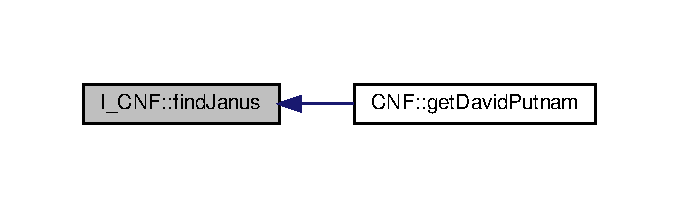
\includegraphics[width=326pt]{d5/d80/struct_i___c_n_f_ac9fd631eda1871653b2d1fdcd55f18a5_icgraph}
\end{center}
\end{figure}
\mbox{\Hypertarget{struct_i___c_n_f_afedf64bb258fd48ea0f811a9f571f0f0}\label{struct_i___c_n_f_afedf64bb258fd48ea0f811a9f571f0f0}} 
\index{I\+\_\+\+C\+NF@{I\+\_\+\+C\+NF}!generate\+C\+NF@{generate\+C\+NF}}
\index{generate\+C\+NF@{generate\+C\+NF}!I\+\_\+\+C\+NF@{I\+\_\+\+C\+NF}}
\subsubsection{\texorpdfstring{generate\+C\+N\+F()}{generateCNF()}}
{\footnotesize\ttfamily shared\+\_\+ptr$<$ \hyperlink{class_node}{Node} $>$ I\+\_\+\+C\+N\+F\+::generate\+C\+NF (\begin{DoxyParamCaption}\item[{shared\+\_\+ptr$<$ \hyperlink{class_node}{Node} $>$}]{origin\+Tree }\end{DoxyParamCaption})}



generate \hyperlink{class_c_n_f}{C\+NF} form based on origin\+Tree, origin\+Tree will be changed, to prevent lost data, use deep copy of \hyperlink{class_node}{Node} 


\begin{DoxyParams}{Parameters}
{\em origin\+Tree} & -\/ \hyperlink{class_node}{Node} pointer, origin tree to convert to \hyperlink{class_c_n_f}{C\+NF} \\
\hline
\end{DoxyParams}
\begin{DoxyReturn}{Returns}
\hyperlink{class_c_n_f}{C\+NF} tree 
\end{DoxyReturn}
\begin{DoxySeeAlso}{See also}
\hyperlink{class_node_a0d22a418a622a24852610fd51910c5eb}{Node\+::copy} 
\end{DoxySeeAlso}
Here is the caller graph for this function\+:\nopagebreak
\begin{figure}[H]
\begin{center}
\leavevmode
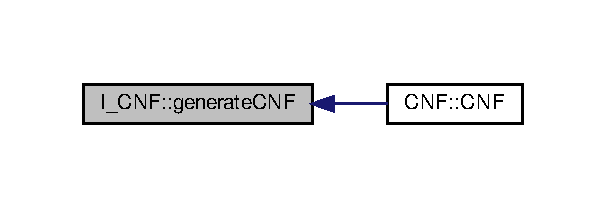
\includegraphics[width=291pt]{d5/d80/struct_i___c_n_f_afedf64bb258fd48ea0f811a9f571f0f0_icgraph}
\end{center}
\end{figure}
\mbox{\Hypertarget{struct_i___c_n_f_ad417af0f07b5e7035c3671dcc3e9f798}\label{struct_i___c_n_f_ad417af0f07b5e7035c3671dcc3e9f798}} 
\index{I\+\_\+\+C\+NF@{I\+\_\+\+C\+NF}!get\+Unique\+List@{get\+Unique\+List}}
\index{get\+Unique\+List@{get\+Unique\+List}!I\+\_\+\+C\+NF@{I\+\_\+\+C\+NF}}
\subsubsection{\texorpdfstring{get\+Unique\+List()}{getUniqueList()}}
{\footnotesize\ttfamily void I\+\_\+\+C\+N\+F\+::get\+Unique\+List (\begin{DoxyParamCaption}\item[{list$<$ shared\+\_\+ptr$<$ \hyperlink{class_node}{Node} $>$ $>$ \&}]{l }\end{DoxyParamCaption})\hspace{0.3cm}{\ttfamily [protected]}}



get unique list of node 


\begin{DoxyParams}[1]{Parameters}
\mbox{\tt in}  & {\em l} & -\/ list of node contains douplicate member \\
\hline
\mbox{\tt out}  & {\em l} & -\/ list of node contains unique member only \\
\hline
\end{DoxyParams}
Here is the caller graph for this function\+:\nopagebreak
\begin{figure}[H]
\begin{center}
\leavevmode
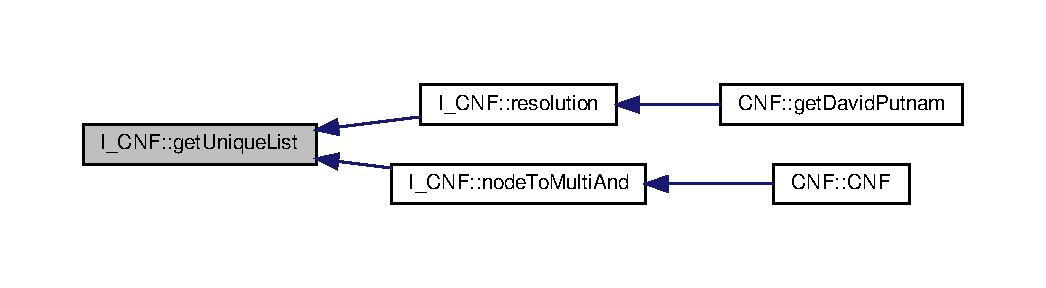
\includegraphics[width=350pt]{d5/d80/struct_i___c_n_f_ad417af0f07b5e7035c3671dcc3e9f798_icgraph}
\end{center}
\end{figure}
\mbox{\Hypertarget{struct_i___c_n_f_a41a7be439cae3ed577a30b3f2742218e}\label{struct_i___c_n_f_a41a7be439cae3ed577a30b3f2742218e}} 
\index{I\+\_\+\+C\+NF@{I\+\_\+\+C\+NF}!is\+Contain@{is\+Contain}}
\index{is\+Contain@{is\+Contain}!I\+\_\+\+C\+NF@{I\+\_\+\+C\+NF}}
\subsubsection{\texorpdfstring{is\+Contain()}{isContain()}}
{\footnotesize\ttfamily bool I\+\_\+\+C\+N\+F\+::is\+Contain (\begin{DoxyParamCaption}\item[{shared\+\_\+ptr$<$ \hyperlink{class_node}{Node} $>$}]{nodes,  }\item[{string}]{v }\end{DoxyParamCaption})\hspace{0.3cm}{\ttfamily [private]}}



check if node contain variable v 


\begin{DoxyParams}{Parameters}
{\em nodes} & -\/ \hyperlink{class_node}{Node}, node to check \\
\hline
{\em v} & -\/ String, variable v \\
\hline
\end{DoxyParams}
\begin{DoxyReturn}{Returns}
True -\/ if node contains variable v ~\newline
 False -\/ if node does not contains variable v 
\end{DoxyReturn}
Here is the caller graph for this function\+:\nopagebreak
\begin{figure}[H]
\begin{center}
\leavevmode
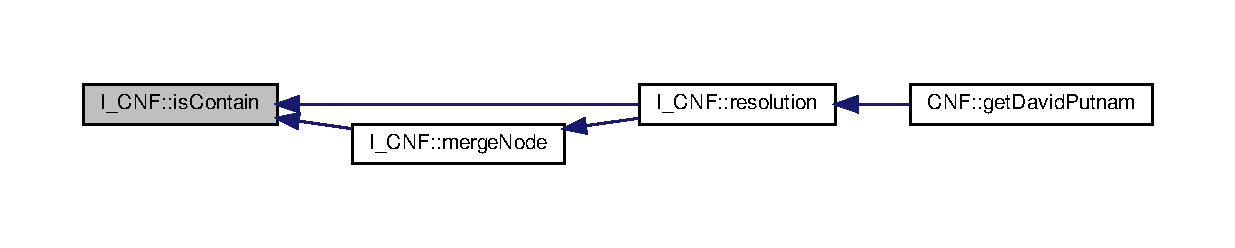
\includegraphics[width=350pt]{d5/d80/struct_i___c_n_f_a41a7be439cae3ed577a30b3f2742218e_icgraph}
\end{center}
\end{figure}
\mbox{\Hypertarget{struct_i___c_n_f_ae9f978965edae4ab57c692544cb72d01}\label{struct_i___c_n_f_ae9f978965edae4ab57c692544cb72d01}} 
\index{I\+\_\+\+C\+NF@{I\+\_\+\+C\+NF}!is\+Useless@{is\+Useless}}
\index{is\+Useless@{is\+Useless}!I\+\_\+\+C\+NF@{I\+\_\+\+C\+NF}}
\subsubsection{\texorpdfstring{is\+Useless()}{isUseless()}}
{\footnotesize\ttfamily bool I\+\_\+\+C\+N\+F\+::is\+Useless (\begin{DoxyParamCaption}\item[{shared\+\_\+ptr$<$ \hyperlink{class_node}{Node} $>$}]{node }\end{DoxyParamCaption})\hspace{0.3cm}{\ttfamily [static]}}



Check if node is useless. 


\begin{DoxyParams}{Parameters}
{\em node} & -\/ \hyperlink{class_multi_or}{Multi\+Or} node \\
\hline
\end{DoxyParams}
\begin{DoxyReturn}{Returns}
True -\/ if node is useless ~\newline
 False -\/ if node is not useless 
\end{DoxyReturn}
Here is the caller graph for this function\+:\nopagebreak
\begin{figure}[H]
\begin{center}
\leavevmode
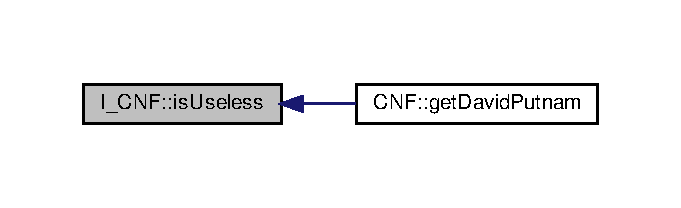
\includegraphics[width=327pt]{d5/d80/struct_i___c_n_f_ae9f978965edae4ab57c692544cb72d01_icgraph}
\end{center}
\end{figure}
\mbox{\Hypertarget{struct_i___c_n_f_a62586e691ebfb00696be6bf9710f4da4}\label{struct_i___c_n_f_a62586e691ebfb00696be6bf9710f4da4}} 
\index{I\+\_\+\+C\+NF@{I\+\_\+\+C\+NF}!merge\+Node@{merge\+Node}}
\index{merge\+Node@{merge\+Node}!I\+\_\+\+C\+NF@{I\+\_\+\+C\+NF}}
\subsubsection{\texorpdfstring{merge\+Node()}{mergeNode()}}
{\footnotesize\ttfamily shared\+\_\+ptr$<$ \hyperlink{class_node}{Node} $>$ I\+\_\+\+C\+N\+F\+::merge\+Node (\begin{DoxyParamCaption}\item[{shared\+\_\+ptr$<$ \hyperlink{class_node}{Node} $>$}]{node1,  }\item[{shared\+\_\+ptr$<$ \hyperlink{class_node}{Node} $>$}]{node2,  }\item[{string}]{v,  }\item[{string}]{not\+\_\+v }\end{DoxyParamCaption})\hspace{0.3cm}{\ttfamily [private]}}



merge two \hyperlink{class_node_a350b631f3a9192bfa23bc266f6b8da02}{Node\+::variables} list. 

This function use for \hyperlink{class_multi_or}{Multi\+Or}, used by \hyperlink{struct_i___c_n_f_a1b3282ebd2d998f5fe3aa3e192346ac1}{I\+\_\+\+C\+N\+F\+::resolution} 
\begin{DoxyParams}{Parameters}
{\em node1} & -\/ first node \\
\hline
{\em node2} & -\/ second node \\
\hline
{\em v} & -\/ string of variable v, upper case \\
\hline
{\em not\+\_\+v} & -\/ string of variable v, lowercase \\
\hline
\end{DoxyParams}
\begin{DoxyReturn}{Returns}
merged \hyperlink{class_node}{Node} 
\end{DoxyReturn}
Here is the call graph for this function\+:\nopagebreak
\begin{figure}[H]
\begin{center}
\leavevmode
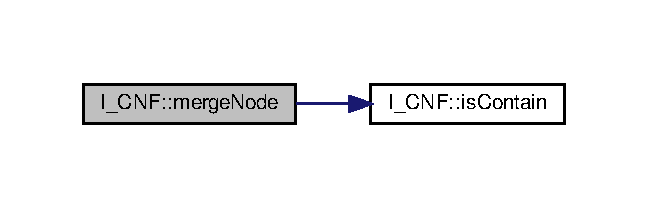
\includegraphics[width=311pt]{d5/d80/struct_i___c_n_f_a62586e691ebfb00696be6bf9710f4da4_cgraph}
\end{center}
\end{figure}
Here is the caller graph for this function\+:\nopagebreak
\begin{figure}[H]
\begin{center}
\leavevmode
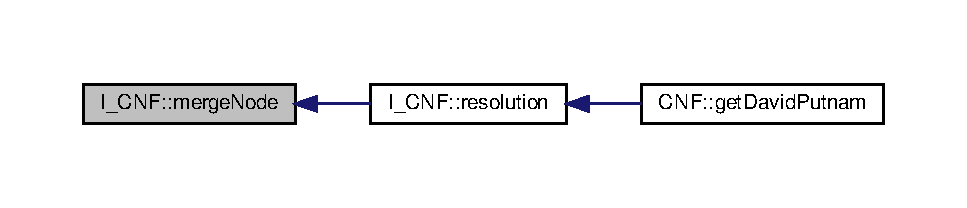
\includegraphics[width=350pt]{d5/d80/struct_i___c_n_f_a62586e691ebfb00696be6bf9710f4da4_icgraph}
\end{center}
\end{figure}
\mbox{\Hypertarget{struct_i___c_n_f_ac0c5ce2bd3edadb60de923b4259cc10b}\label{struct_i___c_n_f_ac0c5ce2bd3edadb60de923b4259cc10b}} 
\index{I\+\_\+\+C\+NF@{I\+\_\+\+C\+NF}!node\+To\+Multi\+And@{node\+To\+Multi\+And}}
\index{node\+To\+Multi\+And@{node\+To\+Multi\+And}!I\+\_\+\+C\+NF@{I\+\_\+\+C\+NF}}
\subsubsection{\texorpdfstring{node\+To\+Multi\+And()}{nodeToMultiAnd()}}
{\footnotesize\ttfamily shared\+\_\+ptr$<$ \hyperlink{class_node}{Node} $>$ I\+\_\+\+C\+N\+F\+::node\+To\+Multi\+And (\begin{DoxyParamCaption}\item[{shared\+\_\+ptr$<$ \hyperlink{class_node}{Node} $>$}]{node }\end{DoxyParamCaption})}



Convert node to \hyperlink{class_multi_and}{Multi\+And}, remove douplicate element and sort element This function are being used after generate\+C\+NF. 


\begin{DoxyParams}{Parameters}
{\em node} & -\/ node to convert \\
\hline
\end{DoxyParams}
\begin{DoxyReturn}{Returns}
\hyperlink{class_multi_and}{Multi\+And} node, with deep of 3 
\end{DoxyReturn}
\begin{DoxySeeAlso}{See also}
\hyperlink{class_node_a73ccf66e577caa428163477f3b4cfe4d}{Node\+::get\+Leaf}, \hyperlink{struct_i___c_n_f_afedf64bb258fd48ea0f811a9f571f0f0}{I\+\_\+\+C\+N\+F\+::generate\+C\+NF} 
\end{DoxySeeAlso}
Here is the call graph for this function\+:\nopagebreak
\begin{figure}[H]
\begin{center}
\leavevmode
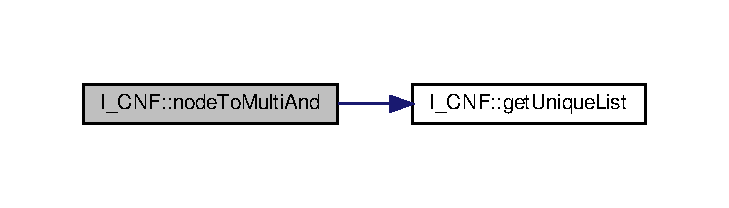
\includegraphics[width=350pt]{d5/d80/struct_i___c_n_f_ac0c5ce2bd3edadb60de923b4259cc10b_cgraph}
\end{center}
\end{figure}
Here is the caller graph for this function\+:\nopagebreak
\begin{figure}[H]
\begin{center}
\leavevmode
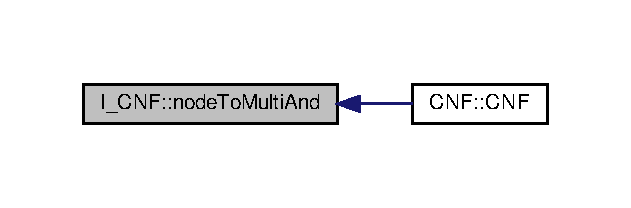
\includegraphics[width=303pt]{d5/d80/struct_i___c_n_f_ac0c5ce2bd3edadb60de923b4259cc10b_icgraph}
\end{center}
\end{figure}
\mbox{\Hypertarget{struct_i___c_n_f_a1b3282ebd2d998f5fe3aa3e192346ac1}\label{struct_i___c_n_f_a1b3282ebd2d998f5fe3aa3e192346ac1}} 
\index{I\+\_\+\+C\+NF@{I\+\_\+\+C\+NF}!resolution@{resolution}}
\index{resolution@{resolution}!I\+\_\+\+C\+NF@{I\+\_\+\+C\+NF}}
\subsubsection{\texorpdfstring{resolution()}{resolution()}}
{\footnotesize\ttfamily \hyperlink{struct_reso}{Reso} I\+\_\+\+C\+N\+F\+::resolution (\begin{DoxyParamCaption}\item[{shared\+\_\+ptr$<$ \hyperlink{class_node}{Node} $>$}]{node,  }\item[{char}]{v }\end{DoxyParamCaption})}



Resolution based on Muliti\+And node and variable v. 


\begin{DoxyParams}{Parameters}
{\em node} & \\
\hline
{\em v} & \\
\hline
\end{DoxyParams}
\begin{DoxyReturn}{Returns}
\hyperlink{struct_reso}{Reso}, contain node Resolution and Subtitute Resolution 
\end{DoxyReturn}
Here is the call graph for this function\+:\nopagebreak
\begin{figure}[H]
\begin{center}
\leavevmode
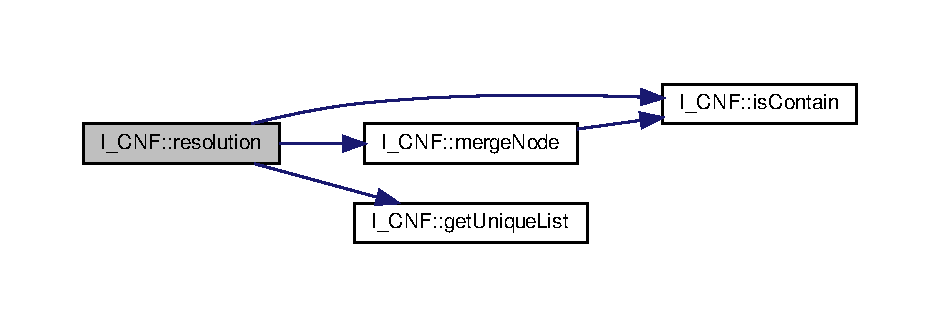
\includegraphics[width=350pt]{d5/d80/struct_i___c_n_f_a1b3282ebd2d998f5fe3aa3e192346ac1_cgraph}
\end{center}
\end{figure}
Here is the caller graph for this function\+:\nopagebreak
\begin{figure}[H]
\begin{center}
\leavevmode
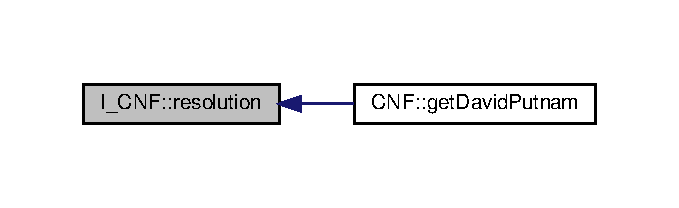
\includegraphics[width=326pt]{d5/d80/struct_i___c_n_f_a1b3282ebd2d998f5fe3aa3e192346ac1_icgraph}
\end{center}
\end{figure}
\mbox{\Hypertarget{struct_i___c_n_f_aa7adb25b5dbb1f4dcddaf56dab338add}\label{struct_i___c_n_f_aa7adb25b5dbb1f4dcddaf56dab338add}} 
\index{I\+\_\+\+C\+NF@{I\+\_\+\+C\+NF}!solve\+Non\+Janus@{solve\+Non\+Janus}}
\index{solve\+Non\+Janus@{solve\+Non\+Janus}!I\+\_\+\+C\+NF@{I\+\_\+\+C\+NF}}
\subsubsection{\texorpdfstring{solve\+Non\+Janus()}{solveNonJanus()}}
{\footnotesize\ttfamily string I\+\_\+\+C\+N\+F\+::solve\+Non\+Janus (\begin{DoxyParamCaption}\item[{shared\+\_\+ptr$<$ \hyperlink{class_node}{Node} $>$}]{node,  }\item[{char}]{v }\end{DoxyParamCaption})}



Solve non-\/janus based on Muliti\+And node and variable v. 


\begin{DoxyParams}[1]{Parameters}
\mbox{\tt in}  & {\em node} & -\/ \hyperlink{class_multi_and}{Multi\+And} \hyperlink{class_node}{Node} pointer to find janus \\
\hline
\mbox{\tt out}  & {\em node} & -\/ node will be filter out if janus have found \\
\hline
 & {\em v} & -\/ String represent for current variable \\
\hline
\end{DoxyParams}
\begin{DoxyReturn}{Returns}
String contains founded janus ~\newline
 Emplty string if janus not found 
\end{DoxyReturn}
Here is the caller graph for this function\+:\nopagebreak
\begin{figure}[H]
\begin{center}
\leavevmode
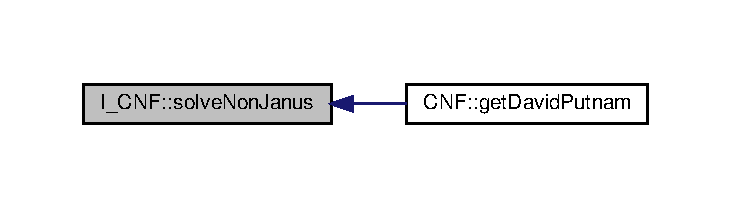
\includegraphics[width=350pt]{d5/d80/struct_i___c_n_f_aa7adb25b5dbb1f4dcddaf56dab338add_icgraph}
\end{center}
\end{figure}


The documentation for this struct was generated from the following files\+:\begin{DoxyCompactItemize}
\item 
src/cnf/\hyperlink{cnf_8h}{cnf.\+h}\item 
src/cnf/\hyperlink{cnf_8cpp}{cnf.\+cpp}\end{DoxyCompactItemize}

\hypertarget{class_implicate}{}\section{Implicate Class Reference}
\label{class_implicate}\index{Implicate@{Implicate}}


{\ttfamily \#include $<$implicate.\+h$>$}



Inheritance diagram for Implicate\+:\nopagebreak
\begin{figure}[H]
\begin{center}
\leavevmode
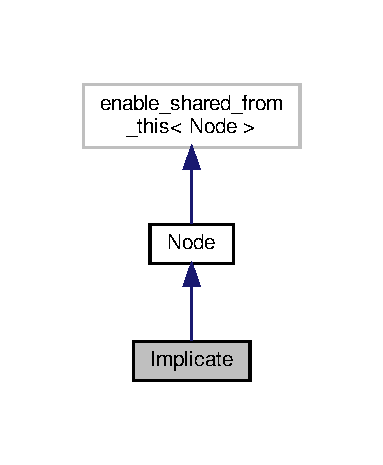
\includegraphics[width=184pt]{db/dcd/class_implicate__inherit__graph}
\end{center}
\end{figure}


Collaboration diagram for Implicate\+:\nopagebreak
\begin{figure}[H]
\begin{center}
\leavevmode
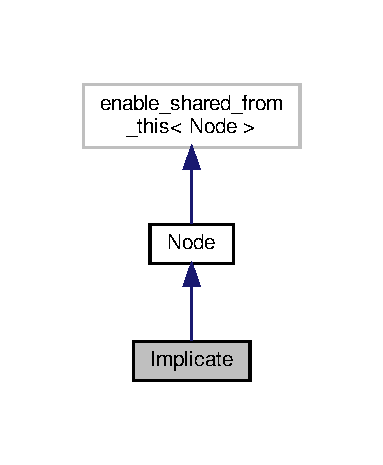
\includegraphics[width=184pt]{d4/d97/class_implicate__coll__graph}
\end{center}
\end{figure}
\subsection*{Public Member Functions}
\begin{DoxyCompactItemize}
\item 
\hyperlink{class_implicate_a7386039d72650d3da8562144b1868722}{Implicate} (shared\+\_\+ptr$<$ \hyperlink{class_node}{Node} $>$ \hyperlink{class_node_a978574f2c08939cfef1041041eb9c5be}{left}=nullptr, shared\+\_\+ptr$<$ \hyperlink{class_node}{Node} $>$ \hyperlink{class_node_af68a851484bce64ed9463a50025df424}{right}=nullptr)
\item 
\hyperlink{class_implicate_a8339c7a4895d95f6c06d7db5714ab8b3}{$\sim$\+Implicate} () override
\item 
bool \hyperlink{class_implicate_a331e1a1fcbe378ef15a3a7f04b7034d5}{get\+Value} (string val\+List) override
\begin{DoxyCompactList}\small\item\em get proposition value \end{DoxyCompactList}\item 
shared\+\_\+ptr$<$ \hyperlink{class_node}{Node} $>$ \hyperlink{class_implicate_a9f3b5d35f552a62ca4a98b4f608a2968}{nandify} (bool is\+Negation) override
\begin{DoxyCompactList}\small\item\em nandify proposition \end{DoxyCompactList}\item 
\hyperlink{proposition_2tableaux_2enum_8h_a70c93904c6a27d228050f922eb4fc3b8}{R\+U\+L\+ES} \hyperlink{class_implicate_aa425e8cb25aec8dd2935346f61ebaefa}{get\+S\+T\+Rule\+Name} (bool is\+Negation) override
\begin{DoxyCompactList}\small\item\em get semantic taubleux rule name \end{DoxyCompactList}\item 
void \hyperlink{class_implicate_aca5eae3d47c318ba413787c7c3a674ce}{get\+S\+T\+Node\+Child} (shared\+\_\+ptr$<$ \hyperlink{class_s_t_node}{S\+T\+Node} $>$ root, long pos, bool is\+Negation) override
\begin{DoxyCompactList}\small\item\em get semantic taubleaux node child (\hyperlink{class_s_t_node_a19ba8bab4660bdeee0e897687b451a8b}{S\+T\+Node.\+left} and \hyperlink{class_s_t_node_a66d06118063fb739058f91c75b725e27}{S\+T\+Node.\+right}) \end{DoxyCompactList}\item 
shared\+\_\+ptr$<$ \hyperlink{class_node}{Node} $>$ \hyperlink{class_implicate_a84e18887eae8891eec583aafaf2bf63d}{cnf\+Filter} (bool is\+Negation=false) override
\begin{DoxyCompactList}\small\item\em in this function node will be \end{DoxyCompactList}\item 
shared\+\_\+ptr$<$ \hyperlink{class_node}{Node} $>$ \hyperlink{class_implicate_a08cf8aa03589f7a34400a5f636f1256a}{copy} () override
\begin{DoxyCompactList}\small\item\em deep copy node \end{DoxyCompactList}\end{DoxyCompactItemize}
\subsection*{Additional Inherited Members}


\subsection{Constructor \& Destructor Documentation}
\mbox{\Hypertarget{class_implicate_a7386039d72650d3da8562144b1868722}\label{class_implicate_a7386039d72650d3da8562144b1868722}} 
\index{Implicate@{Implicate}!Implicate@{Implicate}}
\index{Implicate@{Implicate}!Implicate@{Implicate}}
\subsubsection{\texorpdfstring{Implicate()}{Implicate()}}
{\footnotesize\ttfamily Implicate\+::\+Implicate (\begin{DoxyParamCaption}\item[{shared\+\_\+ptr$<$ \hyperlink{class_node}{Node} $>$}]{left = {\ttfamily nullptr},  }\item[{shared\+\_\+ptr$<$ \hyperlink{class_node}{Node} $>$}]{right = {\ttfamily nullptr} }\end{DoxyParamCaption})\hspace{0.3cm}{\ttfamily [explicit]}}

\mbox{\Hypertarget{class_implicate_a8339c7a4895d95f6c06d7db5714ab8b3}\label{class_implicate_a8339c7a4895d95f6c06d7db5714ab8b3}} 
\index{Implicate@{Implicate}!````~Implicate@{$\sim$\+Implicate}}
\index{````~Implicate@{$\sim$\+Implicate}!Implicate@{Implicate}}
\subsubsection{\texorpdfstring{$\sim$\+Implicate()}{~Implicate()}}
{\footnotesize\ttfamily Implicate\+::$\sim$\+Implicate (\begin{DoxyParamCaption}{ }\end{DoxyParamCaption})\hspace{0.3cm}{\ttfamily [override]}}



\subsection{Member Function Documentation}
\mbox{\Hypertarget{class_implicate_a84e18887eae8891eec583aafaf2bf63d}\label{class_implicate_a84e18887eae8891eec583aafaf2bf63d}} 
\index{Implicate@{Implicate}!cnf\+Filter@{cnf\+Filter}}
\index{cnf\+Filter@{cnf\+Filter}!Implicate@{Implicate}}
\subsubsection{\texorpdfstring{cnf\+Filter()}{cnfFilter()}}
{\footnotesize\ttfamily shared\+\_\+ptr$<$ \hyperlink{class_node}{Node} $>$ Implicate\+::cnf\+Filter (\begin{DoxyParamCaption}\item[{bool}]{is\+Negation = {\ttfamily false} }\end{DoxyParamCaption})\hspace{0.3cm}{\ttfamily [override]}, {\ttfamily [virtual]}}



in this function node will be 


\begin{DoxyItemize}
\item Remove bi-\/implicate
\item Remove implicate
\item Doing the morgan 
\begin{DoxyParams}{Parameters}
{\em is\+Negation} & -\/ check if this node parent is Negation \\
\hline
\end{DoxyParams}
\begin{DoxyReturn}{Returns}
node has been cnf filtered 
\end{DoxyReturn}

\end{DoxyItemize}

Reimplemented from \hyperlink{class_node_ab5b01fd3c4efe0f2eaf7fc41653359b7}{Node}.

Here is the call graph for this function\+:\nopagebreak
\begin{figure}[H]
\begin{center}
\leavevmode
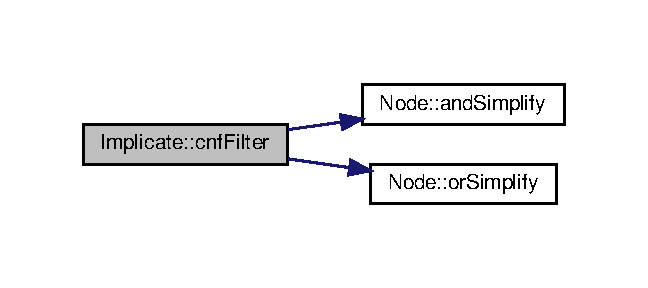
\includegraphics[width=311pt]{de/d28/class_implicate_a84e18887eae8891eec583aafaf2bf63d_cgraph}
\end{center}
\end{figure}
\mbox{\Hypertarget{class_implicate_a08cf8aa03589f7a34400a5f636f1256a}\label{class_implicate_a08cf8aa03589f7a34400a5f636f1256a}} 
\index{Implicate@{Implicate}!copy@{copy}}
\index{copy@{copy}!Implicate@{Implicate}}
\subsubsection{\texorpdfstring{copy()}{copy()}}
{\footnotesize\ttfamily shared\+\_\+ptr$<$ \hyperlink{class_node}{Node} $>$ Implicate\+::copy (\begin{DoxyParamCaption}{ }\end{DoxyParamCaption})\hspace{0.3cm}{\ttfamily [override]}, {\ttfamily [virtual]}}



deep copy node 

\begin{DoxyReturn}{Returns}
a deep copy of node 
\end{DoxyReturn}


Reimplemented from \hyperlink{class_node_a0d22a418a622a24852610fd51910c5eb}{Node}.

\mbox{\Hypertarget{class_implicate_aca5eae3d47c318ba413787c7c3a674ce}\label{class_implicate_aca5eae3d47c318ba413787c7c3a674ce}} 
\index{Implicate@{Implicate}!get\+S\+T\+Node\+Child@{get\+S\+T\+Node\+Child}}
\index{get\+S\+T\+Node\+Child@{get\+S\+T\+Node\+Child}!Implicate@{Implicate}}
\subsubsection{\texorpdfstring{get\+S\+T\+Node\+Child()}{getSTNodeChild()}}
{\footnotesize\ttfamily void Implicate\+::get\+S\+T\+Node\+Child (\begin{DoxyParamCaption}\item[{shared\+\_\+ptr$<$ \hyperlink{class_s_t_node}{S\+T\+Node} $>$}]{root,  }\item[{long}]{pos,  }\item[{bool}]{is\+Negation }\end{DoxyParamCaption})\hspace{0.3cm}{\ttfamily [override]}, {\ttfamily [virtual]}}



get semantic taubleaux node child (\hyperlink{class_s_t_node_a19ba8bab4660bdeee0e897687b451a8b}{S\+T\+Node.\+left} and \hyperlink{class_s_t_node_a66d06118063fb739058f91c75b725e27}{S\+T\+Node.\+right}) 


\begin{DoxyParams}[1]{Parameters}
\mbox{\tt in}  & {\em root} & -\/ \hyperlink{class_s_t_node}{S\+T\+Node} \\
\hline
\mbox{\tt out}  & {\em root} & -\/ \hyperlink{class_s_t_node}{S\+T\+Node} contains child \\
\hline
 & {\em pos} & -\/ position of child \hyperlink{class_node}{Node} of \hyperlink{class_s_t_node_a370cb3b8a6bcd2e488a27d47be4e0920}{S\+T\+Node\+::nodes} list \\
\hline
 & {\em is\+Negation} & -\/ check if this node parent is Negation \\
\hline
\end{DoxyParams}


Reimplemented from \hyperlink{class_node_a1009cb6d84206c2b5eaa86580da59a7c}{Node}.

\mbox{\Hypertarget{class_implicate_aa425e8cb25aec8dd2935346f61ebaefa}\label{class_implicate_aa425e8cb25aec8dd2935346f61ebaefa}} 
\index{Implicate@{Implicate}!get\+S\+T\+Rule\+Name@{get\+S\+T\+Rule\+Name}}
\index{get\+S\+T\+Rule\+Name@{get\+S\+T\+Rule\+Name}!Implicate@{Implicate}}
\subsubsection{\texorpdfstring{get\+S\+T\+Rule\+Name()}{getSTRuleName()}}
{\footnotesize\ttfamily \hyperlink{proposition_2tableaux_2enum_8h_a70c93904c6a27d228050f922eb4fc3b8}{R\+U\+L\+ES} Implicate\+::get\+S\+T\+Rule\+Name (\begin{DoxyParamCaption}\item[{bool}]{is\+Negation }\end{DoxyParamCaption})\hspace{0.3cm}{\ttfamily [override]}, {\ttfamily [virtual]}}



get semantic taubleux rule name 


\begin{DoxyParams}{Parameters}
{\em is\+Negation} & -\/ check if this node parent is Negation \\
\hline
\end{DoxyParams}
\begin{DoxyReturn}{Returns}
R\+U\+L\+ES -\/ semantic taubleaux rule name 
\end{DoxyReturn}


Reimplemented from \hyperlink{class_node_a25b6581950988c2536a392a6874c8072}{Node}.

\mbox{\Hypertarget{class_implicate_a331e1a1fcbe378ef15a3a7f04b7034d5}\label{class_implicate_a331e1a1fcbe378ef15a3a7f04b7034d5}} 
\index{Implicate@{Implicate}!get\+Value@{get\+Value}}
\index{get\+Value@{get\+Value}!Implicate@{Implicate}}
\subsubsection{\texorpdfstring{get\+Value()}{getValue()}}
{\footnotesize\ttfamily bool Implicate\+::get\+Value (\begin{DoxyParamCaption}\item[{string}]{val\+List }\end{DoxyParamCaption})\hspace{0.3cm}{\ttfamily [override]}, {\ttfamily [virtual]}}



get proposition value 


\begin{DoxyParams}{Parameters}
{\em val\+List} & -\/ string contains proposition variable and their value. ~\newline
 e.\+g. \char`\"{}\+A1\+B0\+C1\char`\"{} \\
\hline
\end{DoxyParams}
\begin{DoxyReturn}{Returns}
proposition value 
\end{DoxyReturn}


Reimplemented from \hyperlink{class_node_afd0c2045f3955e02e3aa1e2e987f10b2}{Node}.

\mbox{\Hypertarget{class_implicate_a9f3b5d35f552a62ca4a98b4f608a2968}\label{class_implicate_a9f3b5d35f552a62ca4a98b4f608a2968}} 
\index{Implicate@{Implicate}!nandify@{nandify}}
\index{nandify@{nandify}!Implicate@{Implicate}}
\subsubsection{\texorpdfstring{nandify()}{nandify()}}
{\footnotesize\ttfamily shared\+\_\+ptr$<$ \hyperlink{class_node}{Node} $>$ Implicate\+::nandify (\begin{DoxyParamCaption}\item[{bool}]{is\+Negation }\end{DoxyParamCaption})\hspace{0.3cm}{\ttfamily [override]}, {\ttfamily [virtual]}}



nandify proposition 


\begin{DoxyParams}{Parameters}
{\em is\+Negation} & -\/ check if this node parent is Negation \\
\hline
\end{DoxyParams}
\begin{DoxyReturn}{Returns}
nandified tree 
\end{DoxyReturn}


Reimplemented from \hyperlink{class_node_a3b2e192b59b7e72908af7903c5a4e5c1}{Node}.



The documentation for this class was generated from the following files\+:\begin{DoxyCompactItemize}
\item 
src/notation/\hyperlink{implicate_8h}{implicate.\+h}\item 
src/notation/\hyperlink{implicate_8cpp}{implicate.\+cpp}\end{DoxyCompactItemize}

\hypertarget{classlogging}{}\section{logging Class Reference}
\label{classlogging}\index{logging@{logging}}


{\ttfamily \#include $<$logging.\+h$>$}



Collaboration diagram for logging\+:\nopagebreak
\begin{figure}[H]
\begin{center}
\leavevmode
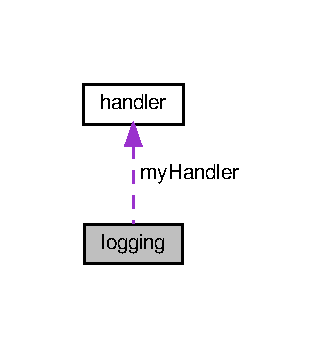
\includegraphics[width=155pt]{d7/d7f/classlogging__coll__graph}
\end{center}
\end{figure}
\subsection*{Public Member Functions}
\begin{DoxyCompactItemize}
\item 
\hyperlink{classlogging_a9fc3278b328fdec4922315d85f772489}{logging} ()
\item 
\hyperlink{classlogging_a38300200148601f298e30b8a84ad686c}{logging} (\hyperlink{classhandler}{handler} $\ast$h)
\item 
\hyperlink{classlogging_aa50e430d72fd366e7f906b61242c658f}{$\sim$logging} ()
\item 
void \hyperlink{classlogging_a3df699bc82c58695050e68f28fa4bf39}{set\+Handler} (\hyperlink{classhandler}{handler} $\ast$new\+Handler)
\item 
void \hyperlink{classlogging_aa15fabd099ea702ad39a8bb82e56d56c}{info} (std\+::string message)
\end{DoxyCompactItemize}
\subsection*{Private Attributes}
\begin{DoxyCompactItemize}
\item 
\hyperlink{classhandler}{handler} $\ast$ \hyperlink{classlogging_a0bd664aa980c8b51e8ebd84c5f6a3901}{my\+Handler}
\end{DoxyCompactItemize}


\subsection{Constructor \& Destructor Documentation}
\mbox{\Hypertarget{classlogging_a9fc3278b328fdec4922315d85f772489}\label{classlogging_a9fc3278b328fdec4922315d85f772489}} 
\index{logging@{logging}!logging@{logging}}
\index{logging@{logging}!logging@{logging}}
\subsubsection{\texorpdfstring{logging()}{logging()}\hspace{0.1cm}{\footnotesize\ttfamily [1/2]}}
{\footnotesize\ttfamily logging\+::logging (\begin{DoxyParamCaption}{ }\end{DoxyParamCaption})}

\mbox{\Hypertarget{classlogging_a38300200148601f298e30b8a84ad686c}\label{classlogging_a38300200148601f298e30b8a84ad686c}} 
\index{logging@{logging}!logging@{logging}}
\index{logging@{logging}!logging@{logging}}
\subsubsection{\texorpdfstring{logging()}{logging()}\hspace{0.1cm}{\footnotesize\ttfamily [2/2]}}
{\footnotesize\ttfamily logging\+::logging (\begin{DoxyParamCaption}\item[{\hyperlink{classhandler}{handler} $\ast$}]{h }\end{DoxyParamCaption})}

\mbox{\Hypertarget{classlogging_aa50e430d72fd366e7f906b61242c658f}\label{classlogging_aa50e430d72fd366e7f906b61242c658f}} 
\index{logging@{logging}!````~logging@{$\sim$logging}}
\index{````~logging@{$\sim$logging}!logging@{logging}}
\subsubsection{\texorpdfstring{$\sim$logging()}{~logging()}}
{\footnotesize\ttfamily logging\+::$\sim$logging (\begin{DoxyParamCaption}{ }\end{DoxyParamCaption})}



\subsection{Member Function Documentation}
\mbox{\Hypertarget{classlogging_aa15fabd099ea702ad39a8bb82e56d56c}\label{classlogging_aa15fabd099ea702ad39a8bb82e56d56c}} 
\index{logging@{logging}!info@{info}}
\index{info@{info}!logging@{logging}}
\subsubsection{\texorpdfstring{info()}{info()}}
{\footnotesize\ttfamily void logging\+::info (\begin{DoxyParamCaption}\item[{std\+::string}]{message }\end{DoxyParamCaption})}

Here is the call graph for this function\+:\nopagebreak
\begin{figure}[H]
\begin{center}
\leavevmode
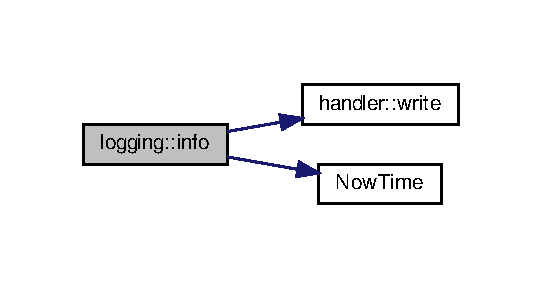
\includegraphics[width=260pt]{d4/d8d/classlogging_aa15fabd099ea702ad39a8bb82e56d56c_cgraph}
\end{center}
\end{figure}
\mbox{\Hypertarget{classlogging_a3df699bc82c58695050e68f28fa4bf39}\label{classlogging_a3df699bc82c58695050e68f28fa4bf39}} 
\index{logging@{logging}!set\+Handler@{set\+Handler}}
\index{set\+Handler@{set\+Handler}!logging@{logging}}
\subsubsection{\texorpdfstring{set\+Handler()}{setHandler()}}
{\footnotesize\ttfamily void logging\+::set\+Handler (\begin{DoxyParamCaption}\item[{\hyperlink{classhandler}{handler} $\ast$}]{new\+Handler }\end{DoxyParamCaption})}



\subsection{Member Data Documentation}
\mbox{\Hypertarget{classlogging_a0bd664aa980c8b51e8ebd84c5f6a3901}\label{classlogging_a0bd664aa980c8b51e8ebd84c5f6a3901}} 
\index{logging@{logging}!my\+Handler@{my\+Handler}}
\index{my\+Handler@{my\+Handler}!logging@{logging}}
\subsubsection{\texorpdfstring{my\+Handler}{myHandler}}
{\footnotesize\ttfamily \hyperlink{classhandler}{handler}$\ast$ logging\+::my\+Handler\hspace{0.3cm}{\ttfamily [private]}}



The documentation for this class was generated from the following files\+:\begin{DoxyCompactItemize}
\item 
src/\hyperlink{logging_8h}{logging.\+h}\item 
src/\hyperlink{logging_8cpp}{logging.\+cpp}\end{DoxyCompactItemize}

\hypertarget{class_multi_and}{}\section{Multi\+And Class Reference}
\label{class_multi_and}\index{Multi\+And@{Multi\+And}}


{\ttfamily \#include $<$multiand.\+h$>$}



Inheritance diagram for Multi\+And\+:\nopagebreak
\begin{figure}[H]
\begin{center}
\leavevmode
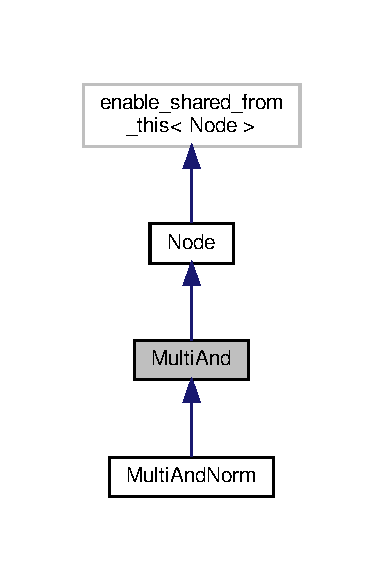
\includegraphics[width=184pt]{db/dd3/class_multi_and__inherit__graph}
\end{center}
\end{figure}


Collaboration diagram for Multi\+And\+:\nopagebreak
\begin{figure}[H]
\begin{center}
\leavevmode
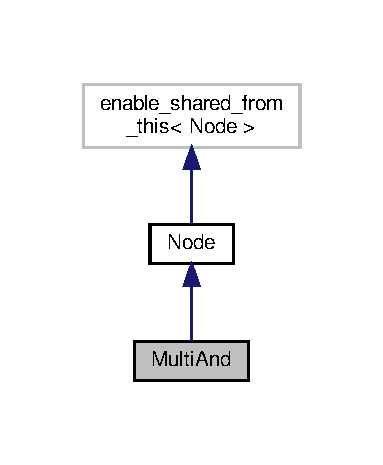
\includegraphics[width=184pt]{d2/d92/class_multi_and__coll__graph}
\end{center}
\end{figure}
\subsection*{Public Member Functions}
\begin{DoxyCompactItemize}
\item 
\hyperlink{class_multi_and_af78c9976d483175359a7c372231b2ac3}{Multi\+And} (list$<$ shared\+\_\+ptr$<$ \hyperlink{class_node}{Node} $>$ $>$ list\+Nodes=list$<$ shared\+\_\+ptr$<$ \hyperlink{class_node}{Node} $>$ $>$())
\item 
\hyperlink{class_multi_and_a2fe5c4c9809102fc779016d608e3f57d}{$\sim$\+Multi\+And} () override
\item 
virtual string \hyperlink{class_multi_and_a035299de4f81beb44a9a5df63b0d5178}{to\+String} () override
\begin{DoxyCompactList}\small\item\em get proposition infix formular \end{DoxyCompactList}\item 
string \hyperlink{class_multi_and_a00dd6431f647c88e28d702dd2afb1c57}{to\+String\+Prefix} () override
\begin{DoxyCompactList}\small\item\em get proposition prefix formular \end{DoxyCompactList}\item 
bool \hyperlink{class_multi_and_a7730036f89cf27cddcf6d2efc293dd9d}{get\+Value} (string val\+List) override
\begin{DoxyCompactList}\small\item\em get proposition value \end{DoxyCompactList}\item 
shared\+\_\+ptr$<$ \hyperlink{class_node}{Node} $>$ \hyperlink{class_multi_and_ad89e8cb08fe1e0793e2e16e837992de2}{copy} () override
\begin{DoxyCompactList}\small\item\em deep copy node \end{DoxyCompactList}\end{DoxyCompactItemize}
\subsection*{Additional Inherited Members}


\subsection{Constructor \& Destructor Documentation}
\mbox{\Hypertarget{class_multi_and_af78c9976d483175359a7c372231b2ac3}\label{class_multi_and_af78c9976d483175359a7c372231b2ac3}} 
\index{Multi\+And@{Multi\+And}!Multi\+And@{Multi\+And}}
\index{Multi\+And@{Multi\+And}!Multi\+And@{Multi\+And}}
\subsubsection{\texorpdfstring{Multi\+And()}{MultiAnd()}}
{\footnotesize\ttfamily Multi\+And\+::\+Multi\+And (\begin{DoxyParamCaption}\item[{list$<$ shared\+\_\+ptr$<$ \hyperlink{class_node}{Node} $>$ $>$}]{list\+Nodes = {\ttfamily list$<$shared\+\_\+ptr$<$\hyperlink{class_node}{Node}$>$~$>$()} }\end{DoxyParamCaption})\hspace{0.3cm}{\ttfamily [explicit]}}

\mbox{\Hypertarget{class_multi_and_a2fe5c4c9809102fc779016d608e3f57d}\label{class_multi_and_a2fe5c4c9809102fc779016d608e3f57d}} 
\index{Multi\+And@{Multi\+And}!````~Multi\+And@{$\sim$\+Multi\+And}}
\index{````~Multi\+And@{$\sim$\+Multi\+And}!Multi\+And@{Multi\+And}}
\subsubsection{\texorpdfstring{$\sim$\+Multi\+And()}{~MultiAnd()}}
{\footnotesize\ttfamily Multi\+And\+::$\sim$\+Multi\+And (\begin{DoxyParamCaption}{ }\end{DoxyParamCaption})\hspace{0.3cm}{\ttfamily [override]}}



\subsection{Member Function Documentation}
\mbox{\Hypertarget{class_multi_and_ad89e8cb08fe1e0793e2e16e837992de2}\label{class_multi_and_ad89e8cb08fe1e0793e2e16e837992de2}} 
\index{Multi\+And@{Multi\+And}!copy@{copy}}
\index{copy@{copy}!Multi\+And@{Multi\+And}}
\subsubsection{\texorpdfstring{copy()}{copy()}}
{\footnotesize\ttfamily shared\+\_\+ptr$<$ \hyperlink{class_node}{Node} $>$ Multi\+And\+::copy (\begin{DoxyParamCaption}{ }\end{DoxyParamCaption})\hspace{0.3cm}{\ttfamily [override]}, {\ttfamily [virtual]}}



deep copy node 

\begin{DoxyReturn}{Returns}
a deep copy of node 
\end{DoxyReturn}


Reimplemented from \hyperlink{class_node_a0d22a418a622a24852610fd51910c5eb}{Node}.



Reimplemented in \hyperlink{class_multi_and_norm_a77cbaf6920daa86d9ddc80b2a839a84f}{Multi\+And\+Norm}.

\mbox{\Hypertarget{class_multi_and_a7730036f89cf27cddcf6d2efc293dd9d}\label{class_multi_and_a7730036f89cf27cddcf6d2efc293dd9d}} 
\index{Multi\+And@{Multi\+And}!get\+Value@{get\+Value}}
\index{get\+Value@{get\+Value}!Multi\+And@{Multi\+And}}
\subsubsection{\texorpdfstring{get\+Value()}{getValue()}}
{\footnotesize\ttfamily bool Multi\+And\+::get\+Value (\begin{DoxyParamCaption}\item[{string}]{val\+List }\end{DoxyParamCaption})\hspace{0.3cm}{\ttfamily [override]}, {\ttfamily [virtual]}}



get proposition value 


\begin{DoxyParams}{Parameters}
{\em val\+List} & -\/ string contains proposition variable and their value. ~\newline
 e.\+g. \char`\"{}\+A1\+B0\+C1\char`\"{} \\
\hline
\end{DoxyParams}
\begin{DoxyReturn}{Returns}
proposition value 
\end{DoxyReturn}


Reimplemented from \hyperlink{class_node_afd0c2045f3955e02e3aa1e2e987f10b2}{Node}.

\mbox{\Hypertarget{class_multi_and_a035299de4f81beb44a9a5df63b0d5178}\label{class_multi_and_a035299de4f81beb44a9a5df63b0d5178}} 
\index{Multi\+And@{Multi\+And}!to\+String@{to\+String}}
\index{to\+String@{to\+String}!Multi\+And@{Multi\+And}}
\subsubsection{\texorpdfstring{to\+String()}{toString()}}
{\footnotesize\ttfamily string Multi\+And\+::to\+String (\begin{DoxyParamCaption}{ }\end{DoxyParamCaption})\hspace{0.3cm}{\ttfamily [override]}, {\ttfamily [virtual]}}



get proposition infix formular 

\begin{DoxyReturn}{Returns}
string of infix proposition 
\end{DoxyReturn}


Reimplemented from \hyperlink{class_node_a0746502074a232243dcac3b96f3ce2d0}{Node}.



Reimplemented in \hyperlink{class_multi_and_norm_a84940789d331007c430096a38f60d124}{Multi\+And\+Norm}.

Here is the caller graph for this function\+:\nopagebreak
\begin{figure}[H]
\begin{center}
\leavevmode
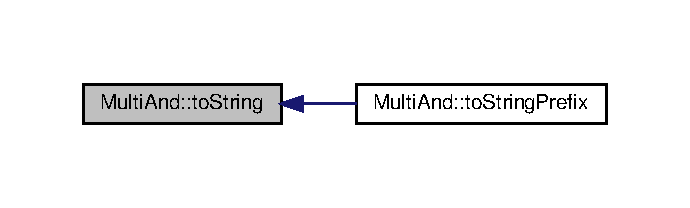
\includegraphics[width=331pt]{d2/d2a/class_multi_and_a035299de4f81beb44a9a5df63b0d5178_icgraph}
\end{center}
\end{figure}
\mbox{\Hypertarget{class_multi_and_a00dd6431f647c88e28d702dd2afb1c57}\label{class_multi_and_a00dd6431f647c88e28d702dd2afb1c57}} 
\index{Multi\+And@{Multi\+And}!to\+String\+Prefix@{to\+String\+Prefix}}
\index{to\+String\+Prefix@{to\+String\+Prefix}!Multi\+And@{Multi\+And}}
\subsubsection{\texorpdfstring{to\+String\+Prefix()}{toStringPrefix()}}
{\footnotesize\ttfamily string Multi\+And\+::to\+String\+Prefix (\begin{DoxyParamCaption}{ }\end{DoxyParamCaption})\hspace{0.3cm}{\ttfamily [override]}, {\ttfamily [virtual]}}



get proposition prefix formular 

\begin{DoxyReturn}{Returns}
string of prefix proposition 
\end{DoxyReturn}


Reimplemented from \hyperlink{class_node_a815b062345cf2bb42717bd16dc99ea27}{Node}.

Here is the call graph for this function\+:\nopagebreak
\begin{figure}[H]
\begin{center}
\leavevmode
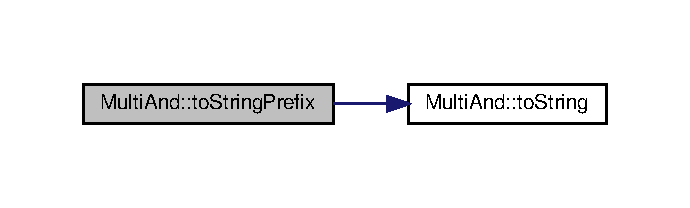
\includegraphics[width=331pt]{d2/d2a/class_multi_and_a00dd6431f647c88e28d702dd2afb1c57_cgraph}
\end{center}
\end{figure}


The documentation for this class was generated from the following files\+:\begin{DoxyCompactItemize}
\item 
src/notation/\hyperlink{multiand_8h}{multiand.\+h}\item 
src/notation/\hyperlink{multiand_8cpp}{multiand.\+cpp}\end{DoxyCompactItemize}

\hypertarget{class_multi_and_norm}{}\section{Multi\+And\+Norm Class Reference}
\label{class_multi_and_norm}\index{Multi\+And\+Norm@{Multi\+And\+Norm}}


{\ttfamily \#include $<$multiand.\+h$>$}



Inheritance diagram for Multi\+And\+Norm\+:\nopagebreak
\begin{figure}[H]
\begin{center}
\leavevmode
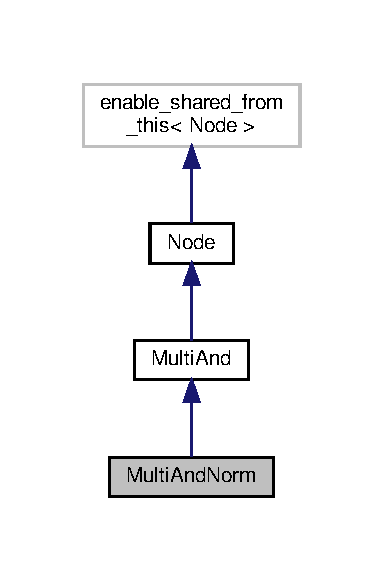
\includegraphics[width=184pt]{df/d77/class_multi_and_norm__inherit__graph}
\end{center}
\end{figure}


Collaboration diagram for Multi\+And\+Norm\+:\nopagebreak
\begin{figure}[H]
\begin{center}
\leavevmode
\includegraphics[width=184pt]{da/dfa/class_multi_and_norm__coll__graph}
\end{center}
\end{figure}
\subsection*{Public Member Functions}
\begin{DoxyCompactItemize}
\item 
\hyperlink{class_multi_and_norm_aee4c9190024a62f701bd02155115fbf0}{Multi\+And\+Norm} (list$<$ shared\+\_\+ptr$<$ \hyperlink{class_node}{Node} $>$ $>$ list\+Nodes=list$<$ shared\+\_\+ptr$<$ \hyperlink{class_node}{Node} $>$ $>$())
\item 
\hyperlink{class_multi_and_norm_a3aec280d3f9c2df9ed0eb91e61f8bb4f}{$\sim$\+Multi\+And\+Norm} () override
\item 
string \hyperlink{class_multi_and_norm_a84940789d331007c430096a38f60d124}{to\+String} () override
\begin{DoxyCompactList}\small\item\em get proposition infix formular \end{DoxyCompactList}\item 
shared\+\_\+ptr$<$ \hyperlink{class_node}{Node} $>$ \hyperlink{class_multi_and_norm_a77cbaf6920daa86d9ddc80b2a839a84f}{copy} () override
\begin{DoxyCompactList}\small\item\em deep copy node \end{DoxyCompactList}\end{DoxyCompactItemize}
\subsection*{Additional Inherited Members}


\subsection{Constructor \& Destructor Documentation}
\mbox{\Hypertarget{class_multi_and_norm_aee4c9190024a62f701bd02155115fbf0}\label{class_multi_and_norm_aee4c9190024a62f701bd02155115fbf0}} 
\index{Multi\+And\+Norm@{Multi\+And\+Norm}!Multi\+And\+Norm@{Multi\+And\+Norm}}
\index{Multi\+And\+Norm@{Multi\+And\+Norm}!Multi\+And\+Norm@{Multi\+And\+Norm}}
\subsubsection{\texorpdfstring{Multi\+And\+Norm()}{MultiAndNorm()}}
{\footnotesize\ttfamily Multi\+And\+Norm\+::\+Multi\+And\+Norm (\begin{DoxyParamCaption}\item[{list$<$ shared\+\_\+ptr$<$ \hyperlink{class_node}{Node} $>$ $>$}]{list\+Nodes = {\ttfamily list$<$shared\+\_\+ptr$<$\hyperlink{class_node}{Node}$>$~$>$()} }\end{DoxyParamCaption})\hspace{0.3cm}{\ttfamily [explicit]}}

\mbox{\Hypertarget{class_multi_and_norm_a3aec280d3f9c2df9ed0eb91e61f8bb4f}\label{class_multi_and_norm_a3aec280d3f9c2df9ed0eb91e61f8bb4f}} 
\index{Multi\+And\+Norm@{Multi\+And\+Norm}!````~Multi\+And\+Norm@{$\sim$\+Multi\+And\+Norm}}
\index{````~Multi\+And\+Norm@{$\sim$\+Multi\+And\+Norm}!Multi\+And\+Norm@{Multi\+And\+Norm}}
\subsubsection{\texorpdfstring{$\sim$\+Multi\+And\+Norm()}{~MultiAndNorm()}}
{\footnotesize\ttfamily Multi\+And\+Norm\+::$\sim$\+Multi\+And\+Norm (\begin{DoxyParamCaption}{ }\end{DoxyParamCaption})\hspace{0.3cm}{\ttfamily [override]}}



\subsection{Member Function Documentation}
\mbox{\Hypertarget{class_multi_and_norm_a77cbaf6920daa86d9ddc80b2a839a84f}\label{class_multi_and_norm_a77cbaf6920daa86d9ddc80b2a839a84f}} 
\index{Multi\+And\+Norm@{Multi\+And\+Norm}!copy@{copy}}
\index{copy@{copy}!Multi\+And\+Norm@{Multi\+And\+Norm}}
\subsubsection{\texorpdfstring{copy()}{copy()}}
{\footnotesize\ttfamily shared\+\_\+ptr$<$ \hyperlink{class_node}{Node} $>$ Multi\+And\+Norm\+::copy (\begin{DoxyParamCaption}{ }\end{DoxyParamCaption})\hspace{0.3cm}{\ttfamily [override]}, {\ttfamily [virtual]}}



deep copy node 

\begin{DoxyReturn}{Returns}
a deep copy of node 
\end{DoxyReturn}


Reimplemented from \hyperlink{class_multi_and_ad89e8cb08fe1e0793e2e16e837992de2}{Multi\+And}.

\mbox{\Hypertarget{class_multi_and_norm_a84940789d331007c430096a38f60d124}\label{class_multi_and_norm_a84940789d331007c430096a38f60d124}} 
\index{Multi\+And\+Norm@{Multi\+And\+Norm}!to\+String@{to\+String}}
\index{to\+String@{to\+String}!Multi\+And\+Norm@{Multi\+And\+Norm}}
\subsubsection{\texorpdfstring{to\+String()}{toString()}}
{\footnotesize\ttfamily string Multi\+And\+Norm\+::to\+String (\begin{DoxyParamCaption}{ }\end{DoxyParamCaption})\hspace{0.3cm}{\ttfamily [override]}, {\ttfamily [virtual]}}



get proposition infix formular 

\begin{DoxyReturn}{Returns}
string of infix proposition 
\end{DoxyReturn}


Reimplemented from \hyperlink{class_multi_and_a035299de4f81beb44a9a5df63b0d5178}{Multi\+And}.



The documentation for this class was generated from the following files\+:\begin{DoxyCompactItemize}
\item 
src/notation/\hyperlink{multiand_8h}{multiand.\+h}\item 
src/notation/\hyperlink{multiand_8cpp}{multiand.\+cpp}\end{DoxyCompactItemize}

\hypertarget{class_multi_or}{}\section{Multi\+Or Class Reference}
\label{class_multi_or}\index{Multi\+Or@{Multi\+Or}}


{\ttfamily \#include $<$multior.\+h$>$}



Inheritance diagram for Multi\+Or\+:\nopagebreak
\begin{figure}[H]
\begin{center}
\leavevmode
\includegraphics[width=184pt]{d3/d60/class_multi_or__inherit__graph}
\end{center}
\end{figure}


Collaboration diagram for Multi\+Or\+:\nopagebreak
\begin{figure}[H]
\begin{center}
\leavevmode
\includegraphics[width=184pt]{df/dcb/class_multi_or__coll__graph}
\end{center}
\end{figure}
\subsection*{Public Member Functions}
\begin{DoxyCompactItemize}
\item 
\hyperlink{class_multi_or_a55dd7025f9f40187496f481f252e33dc}{Multi\+Or} (list$<$ shared\+\_\+ptr$<$ \hyperlink{class_node}{Node} $>$ $>$ list\+Nodes=list$<$ shared\+\_\+ptr$<$ \hyperlink{class_node}{Node} $>$ $>$())
\item 
\hyperlink{class_multi_or_a17ce7a33d4fe548dca2db45a59202057}{Multi\+Or} (shared\+\_\+ptr$<$ \hyperlink{class_node}{Node} $>$ node)
\item 
\hyperlink{class_multi_or_a4f0161febe9e9fe9d4fc44708369de51}{$\sim$\+Multi\+Or} () override
\item 
string \hyperlink{class_multi_or_ade4d5f7db13aca1020dba2396ef00dd7}{to\+String} () override
\begin{DoxyCompactList}\small\item\em get proposition infix formular \end{DoxyCompactList}\item 
string \hyperlink{class_multi_or_a80405614a8a8db0992c35a70f36aa025}{to\+String\+Prefix} () override
\begin{DoxyCompactList}\small\item\em get proposition prefix formular \end{DoxyCompactList}\item 
bool \hyperlink{class_multi_or_a7146240d304444ee0da5c949c584971e}{get\+Value} (string val\+List) override
\begin{DoxyCompactList}\small\item\em get proposition value \end{DoxyCompactList}\item 
shared\+\_\+ptr$<$ \hyperlink{class_node}{Node} $>$ \hyperlink{class_multi_or_a9a81647d40f86c825fdb1513f1b3f30c}{copy} () override
\begin{DoxyCompactList}\small\item\em deep copy node \end{DoxyCompactList}\end{DoxyCompactItemize}
\subsection*{Additional Inherited Members}


\subsection{Constructor \& Destructor Documentation}
\mbox{\Hypertarget{class_multi_or_a55dd7025f9f40187496f481f252e33dc}\label{class_multi_or_a55dd7025f9f40187496f481f252e33dc}} 
\index{Multi\+Or@{Multi\+Or}!Multi\+Or@{Multi\+Or}}
\index{Multi\+Or@{Multi\+Or}!Multi\+Or@{Multi\+Or}}
\subsubsection{\texorpdfstring{Multi\+Or()}{MultiOr()}\hspace{0.1cm}{\footnotesize\ttfamily [1/2]}}
{\footnotesize\ttfamily Multi\+Or\+::\+Multi\+Or (\begin{DoxyParamCaption}\item[{list$<$ shared\+\_\+ptr$<$ \hyperlink{class_node}{Node} $>$ $>$}]{list\+Nodes = {\ttfamily list$<$shared\+\_\+ptr$<$\hyperlink{class_node}{Node}$>$~$>$()} }\end{DoxyParamCaption})\hspace{0.3cm}{\ttfamily [explicit]}}

\mbox{\Hypertarget{class_multi_or_a17ce7a33d4fe548dca2db45a59202057}\label{class_multi_or_a17ce7a33d4fe548dca2db45a59202057}} 
\index{Multi\+Or@{Multi\+Or}!Multi\+Or@{Multi\+Or}}
\index{Multi\+Or@{Multi\+Or}!Multi\+Or@{Multi\+Or}}
\subsubsection{\texorpdfstring{Multi\+Or()}{MultiOr()}\hspace{0.1cm}{\footnotesize\ttfamily [2/2]}}
{\footnotesize\ttfamily Multi\+Or\+::\+Multi\+Or (\begin{DoxyParamCaption}\item[{shared\+\_\+ptr$<$ \hyperlink{class_node}{Node} $>$}]{node }\end{DoxyParamCaption})\hspace{0.3cm}{\ttfamily [explicit]}}

\mbox{\Hypertarget{class_multi_or_a4f0161febe9e9fe9d4fc44708369de51}\label{class_multi_or_a4f0161febe9e9fe9d4fc44708369de51}} 
\index{Multi\+Or@{Multi\+Or}!````~Multi\+Or@{$\sim$\+Multi\+Or}}
\index{````~Multi\+Or@{$\sim$\+Multi\+Or}!Multi\+Or@{Multi\+Or}}
\subsubsection{\texorpdfstring{$\sim$\+Multi\+Or()}{~MultiOr()}}
{\footnotesize\ttfamily Multi\+Or\+::$\sim$\+Multi\+Or (\begin{DoxyParamCaption}{ }\end{DoxyParamCaption})\hspace{0.3cm}{\ttfamily [override]}}



\subsection{Member Function Documentation}
\mbox{\Hypertarget{class_multi_or_a9a81647d40f86c825fdb1513f1b3f30c}\label{class_multi_or_a9a81647d40f86c825fdb1513f1b3f30c}} 
\index{Multi\+Or@{Multi\+Or}!copy@{copy}}
\index{copy@{copy}!Multi\+Or@{Multi\+Or}}
\subsubsection{\texorpdfstring{copy()}{copy()}}
{\footnotesize\ttfamily shared\+\_\+ptr$<$ \hyperlink{class_node}{Node} $>$ Multi\+Or\+::copy (\begin{DoxyParamCaption}{ }\end{DoxyParamCaption})\hspace{0.3cm}{\ttfamily [override]}, {\ttfamily [virtual]}}



deep copy node 

\begin{DoxyReturn}{Returns}
a deep copy of node 
\end{DoxyReturn}


Reimplemented from \hyperlink{class_node_a0d22a418a622a24852610fd51910c5eb}{Node}.



Reimplemented in \hyperlink{class_multi_or_norm_a030bc7807678c834b467daa7a3a8dab5}{Multi\+Or\+Norm}.

\mbox{\Hypertarget{class_multi_or_a7146240d304444ee0da5c949c584971e}\label{class_multi_or_a7146240d304444ee0da5c949c584971e}} 
\index{Multi\+Or@{Multi\+Or}!get\+Value@{get\+Value}}
\index{get\+Value@{get\+Value}!Multi\+Or@{Multi\+Or}}
\subsubsection{\texorpdfstring{get\+Value()}{getValue()}}
{\footnotesize\ttfamily bool Multi\+Or\+::get\+Value (\begin{DoxyParamCaption}\item[{string}]{val\+List }\end{DoxyParamCaption})\hspace{0.3cm}{\ttfamily [override]}, {\ttfamily [virtual]}}



get proposition value 


\begin{DoxyParams}{Parameters}
{\em val\+List} & -\/ string contains proposition variable and their value. ~\newline
 e.\+g. \char`\"{}\+A1\+B0\+C1\char`\"{} \\
\hline
\end{DoxyParams}
\begin{DoxyReturn}{Returns}
proposition value 
\end{DoxyReturn}


Reimplemented from \hyperlink{class_node_afd0c2045f3955e02e3aa1e2e987f10b2}{Node}.

\mbox{\Hypertarget{class_multi_or_ade4d5f7db13aca1020dba2396ef00dd7}\label{class_multi_or_ade4d5f7db13aca1020dba2396ef00dd7}} 
\index{Multi\+Or@{Multi\+Or}!to\+String@{to\+String}}
\index{to\+String@{to\+String}!Multi\+Or@{Multi\+Or}}
\subsubsection{\texorpdfstring{to\+String()}{toString()}}
{\footnotesize\ttfamily string Multi\+Or\+::to\+String (\begin{DoxyParamCaption}{ }\end{DoxyParamCaption})\hspace{0.3cm}{\ttfamily [override]}, {\ttfamily [virtual]}}



get proposition infix formular 

\begin{DoxyReturn}{Returns}
string of infix proposition 
\end{DoxyReturn}


Reimplemented from \hyperlink{class_node_a0746502074a232243dcac3b96f3ce2d0}{Node}.



Reimplemented in \hyperlink{class_multi_or_norm_ad70e2ca31478183da21ee1995964c2c3}{Multi\+Or\+Norm}.

Here is the caller graph for this function\+:\nopagebreak
\begin{figure}[H]
\begin{center}
\leavevmode
\includegraphics[width=317pt]{dd/d61/class_multi_or_ade4d5f7db13aca1020dba2396ef00dd7_icgraph}
\end{center}
\end{figure}
\mbox{\Hypertarget{class_multi_or_a80405614a8a8db0992c35a70f36aa025}\label{class_multi_or_a80405614a8a8db0992c35a70f36aa025}} 
\index{Multi\+Or@{Multi\+Or}!to\+String\+Prefix@{to\+String\+Prefix}}
\index{to\+String\+Prefix@{to\+String\+Prefix}!Multi\+Or@{Multi\+Or}}
\subsubsection{\texorpdfstring{to\+String\+Prefix()}{toStringPrefix()}}
{\footnotesize\ttfamily string Multi\+Or\+::to\+String\+Prefix (\begin{DoxyParamCaption}{ }\end{DoxyParamCaption})\hspace{0.3cm}{\ttfamily [override]}, {\ttfamily [virtual]}}



get proposition prefix formular 

\begin{DoxyReturn}{Returns}
string of prefix proposition 
\end{DoxyReturn}


Reimplemented from \hyperlink{class_node_a815b062345cf2bb42717bd16dc99ea27}{Node}.

Here is the call graph for this function\+:\nopagebreak
\begin{figure}[H]
\begin{center}
\leavevmode
\includegraphics[width=317pt]{dd/d61/class_multi_or_a80405614a8a8db0992c35a70f36aa025_cgraph}
\end{center}
\end{figure}


The documentation for this class was generated from the following files\+:\begin{DoxyCompactItemize}
\item 
src/notation/\hyperlink{multior_8h}{multior.\+h}\item 
src/notation/\hyperlink{multior_8cpp}{multior.\+cpp}\end{DoxyCompactItemize}

\hypertarget{class_multi_or_norm}{}\section{Multi\+Or\+Norm Class Reference}
\label{class_multi_or_norm}\index{Multi\+Or\+Norm@{Multi\+Or\+Norm}}


{\ttfamily \#include $<$multior.\+h$>$}



Inheritance diagram for Multi\+Or\+Norm\+:\nopagebreak
\begin{figure}[H]
\begin{center}
\leavevmode
\includegraphics[width=184pt]{d2/d69/class_multi_or_norm__inherit__graph}
\end{center}
\end{figure}


Collaboration diagram for Multi\+Or\+Norm\+:\nopagebreak
\begin{figure}[H]
\begin{center}
\leavevmode
\includegraphics[width=184pt]{d9/d73/class_multi_or_norm__coll__graph}
\end{center}
\end{figure}
\subsection*{Public Member Functions}
\begin{DoxyCompactItemize}
\item 
\hyperlink{class_multi_or_norm_ae11a281782c23c8a3675d6abc5b3bfbc}{Multi\+Or\+Norm} (list$<$ shared\+\_\+ptr$<$ \hyperlink{class_node}{Node} $>$ $>$ list\+Nodes=list$<$ shared\+\_\+ptr$<$ \hyperlink{class_node}{Node} $>$ $>$())
\item 
\hyperlink{class_multi_or_norm_a43f3ee64ab919f4c85ecdda2a92bef00}{Multi\+Or\+Norm} (shared\+\_\+ptr$<$ \hyperlink{class_node}{Node} $>$ node=nullptr)
\item 
\hyperlink{class_multi_or_norm_a8de0c4794574f93dd2131075943f4209}{$\sim$\+Multi\+Or\+Norm} () override
\item 
string \hyperlink{class_multi_or_norm_ad70e2ca31478183da21ee1995964c2c3}{to\+String} () override
\begin{DoxyCompactList}\small\item\em get proposition infix formular \end{DoxyCompactList}\item 
shared\+\_\+ptr$<$ \hyperlink{class_node}{Node} $>$ \hyperlink{class_multi_or_norm_a030bc7807678c834b467daa7a3a8dab5}{copy} () override
\begin{DoxyCompactList}\small\item\em deep copy node \end{DoxyCompactList}\end{DoxyCompactItemize}
\subsection*{Additional Inherited Members}


\subsection{Constructor \& Destructor Documentation}
\mbox{\Hypertarget{class_multi_or_norm_ae11a281782c23c8a3675d6abc5b3bfbc}\label{class_multi_or_norm_ae11a281782c23c8a3675d6abc5b3bfbc}} 
\index{Multi\+Or\+Norm@{Multi\+Or\+Norm}!Multi\+Or\+Norm@{Multi\+Or\+Norm}}
\index{Multi\+Or\+Norm@{Multi\+Or\+Norm}!Multi\+Or\+Norm@{Multi\+Or\+Norm}}
\subsubsection{\texorpdfstring{Multi\+Or\+Norm()}{MultiOrNorm()}\hspace{0.1cm}{\footnotesize\ttfamily [1/2]}}
{\footnotesize\ttfamily Multi\+Or\+Norm\+::\+Multi\+Or\+Norm (\begin{DoxyParamCaption}\item[{list$<$ shared\+\_\+ptr$<$ \hyperlink{class_node}{Node} $>$ $>$}]{list\+Nodes = {\ttfamily list$<$shared\+\_\+ptr$<$\hyperlink{class_node}{Node}$>$~$>$()} }\end{DoxyParamCaption})\hspace{0.3cm}{\ttfamily [explicit]}}

\mbox{\Hypertarget{class_multi_or_norm_a43f3ee64ab919f4c85ecdda2a92bef00}\label{class_multi_or_norm_a43f3ee64ab919f4c85ecdda2a92bef00}} 
\index{Multi\+Or\+Norm@{Multi\+Or\+Norm}!Multi\+Or\+Norm@{Multi\+Or\+Norm}}
\index{Multi\+Or\+Norm@{Multi\+Or\+Norm}!Multi\+Or\+Norm@{Multi\+Or\+Norm}}
\subsubsection{\texorpdfstring{Multi\+Or\+Norm()}{MultiOrNorm()}\hspace{0.1cm}{\footnotesize\ttfamily [2/2]}}
{\footnotesize\ttfamily Multi\+Or\+Norm\+::\+Multi\+Or\+Norm (\begin{DoxyParamCaption}\item[{shared\+\_\+ptr$<$ \hyperlink{class_node}{Node} $>$}]{node = {\ttfamily nullptr} }\end{DoxyParamCaption})\hspace{0.3cm}{\ttfamily [explicit]}}

\mbox{\Hypertarget{class_multi_or_norm_a8de0c4794574f93dd2131075943f4209}\label{class_multi_or_norm_a8de0c4794574f93dd2131075943f4209}} 
\index{Multi\+Or\+Norm@{Multi\+Or\+Norm}!````~Multi\+Or\+Norm@{$\sim$\+Multi\+Or\+Norm}}
\index{````~Multi\+Or\+Norm@{$\sim$\+Multi\+Or\+Norm}!Multi\+Or\+Norm@{Multi\+Or\+Norm}}
\subsubsection{\texorpdfstring{$\sim$\+Multi\+Or\+Norm()}{~MultiOrNorm()}}
{\footnotesize\ttfamily Multi\+Or\+Norm\+::$\sim$\+Multi\+Or\+Norm (\begin{DoxyParamCaption}{ }\end{DoxyParamCaption})\hspace{0.3cm}{\ttfamily [override]}}



\subsection{Member Function Documentation}
\mbox{\Hypertarget{class_multi_or_norm_a030bc7807678c834b467daa7a3a8dab5}\label{class_multi_or_norm_a030bc7807678c834b467daa7a3a8dab5}} 
\index{Multi\+Or\+Norm@{Multi\+Or\+Norm}!copy@{copy}}
\index{copy@{copy}!Multi\+Or\+Norm@{Multi\+Or\+Norm}}
\subsubsection{\texorpdfstring{copy()}{copy()}}
{\footnotesize\ttfamily shared\+\_\+ptr$<$ \hyperlink{class_node}{Node} $>$ Multi\+Or\+Norm\+::copy (\begin{DoxyParamCaption}{ }\end{DoxyParamCaption})\hspace{0.3cm}{\ttfamily [override]}, {\ttfamily [virtual]}}



deep copy node 

\begin{DoxyReturn}{Returns}
a deep copy of node 
\end{DoxyReturn}


Reimplemented from \hyperlink{class_multi_or_a9a81647d40f86c825fdb1513f1b3f30c}{Multi\+Or}.

\mbox{\Hypertarget{class_multi_or_norm_ad70e2ca31478183da21ee1995964c2c3}\label{class_multi_or_norm_ad70e2ca31478183da21ee1995964c2c3}} 
\index{Multi\+Or\+Norm@{Multi\+Or\+Norm}!to\+String@{to\+String}}
\index{to\+String@{to\+String}!Multi\+Or\+Norm@{Multi\+Or\+Norm}}
\subsubsection{\texorpdfstring{to\+String()}{toString()}}
{\footnotesize\ttfamily string Multi\+Or\+Norm\+::to\+String (\begin{DoxyParamCaption}{ }\end{DoxyParamCaption})\hspace{0.3cm}{\ttfamily [override]}, {\ttfamily [virtual]}}



get proposition infix formular 

\begin{DoxyReturn}{Returns}
string of infix proposition 
\end{DoxyReturn}


Reimplemented from \hyperlink{class_multi_or_ade4d5f7db13aca1020dba2396ef00dd7}{Multi\+Or}.



The documentation for this class was generated from the following files\+:\begin{DoxyCompactItemize}
\item 
src/notation/\hyperlink{multior_8h}{multior.\+h}\item 
src/notation/\hyperlink{multior_8cpp}{multior.\+cpp}\end{DoxyCompactItemize}

\hypertarget{class_n_and}{}\section{N\+And Class Reference}
\label{class_n_and}\index{N\+And@{N\+And}}


{\ttfamily \#include $<$nand.\+h$>$}



Inheritance diagram for N\+And\+:\nopagebreak
\begin{figure}[H]
\begin{center}
\leavevmode
\includegraphics[width=184pt]{de/dc5/class_n_and__inherit__graph}
\end{center}
\end{figure}


Collaboration diagram for N\+And\+:\nopagebreak
\begin{figure}[H]
\begin{center}
\leavevmode
\includegraphics[width=184pt]{d0/d12/class_n_and__coll__graph}
\end{center}
\end{figure}
\subsection*{Public Member Functions}
\begin{DoxyCompactItemize}
\item 
\hyperlink{class_n_and_a5e73ac719f793d02a10cd0fc6931808f}{N\+And} (shared\+\_\+ptr$<$ \hyperlink{class_node}{Node} $>$ l=nullptr, shared\+\_\+ptr$<$ \hyperlink{class_node}{Node} $>$ r=nullptr)
\item 
\hyperlink{class_n_and_a472d8c586ec989b998d6b182ed581a96}{$\sim$\+N\+And} () override
\item 
bool \hyperlink{class_n_and_a9eb3a117e8d30f11ebe25e932d387265}{get\+Value} (string val\+List) override
\begin{DoxyCompactList}\small\item\em get proposition value \end{DoxyCompactList}\item 
shared\+\_\+ptr$<$ \hyperlink{class_node}{Node} $>$ \hyperlink{class_n_and_ae60ecc244dd83bfdcc7eada4957890d8}{nandify} (bool is\+Negation) override
\begin{DoxyCompactList}\small\item\em nandify proposition \end{DoxyCompactList}\item 
\hyperlink{proposition_2tableaux_2enum_8h_a70c93904c6a27d228050f922eb4fc3b8}{R\+U\+L\+ES} \hyperlink{class_n_and_a8570a747f7f4aec32bb962227749566f}{get\+S\+T\+Rule\+Name} (bool is\+Negation) override
\begin{DoxyCompactList}\small\item\em get semantic taubleux rule name \end{DoxyCompactList}\item 
void \hyperlink{class_n_and_a3ccedba07752a2457a593035b33535e1}{get\+S\+T\+Node\+Child} (shared\+\_\+ptr$<$ \hyperlink{class_s_t_node}{S\+T\+Node} $>$ root, long pos, bool is\+Negation) override
\begin{DoxyCompactList}\small\item\em get semantic taubleaux node child (\hyperlink{class_s_t_node_a19ba8bab4660bdeee0e897687b451a8b}{S\+T\+Node.\+left} and \hyperlink{class_s_t_node_a66d06118063fb739058f91c75b725e27}{S\+T\+Node.\+right}) \end{DoxyCompactList}\item 
shared\+\_\+ptr$<$ \hyperlink{class_node}{Node} $>$ \hyperlink{class_n_and_a2df64f0858e90841201a2acaf50ac587}{cnf\+Filter} (bool is\+Negation=false) override
\begin{DoxyCompactList}\small\item\em in this function node will be \end{DoxyCompactList}\item 
shared\+\_\+ptr$<$ \hyperlink{class_node}{Node} $>$ \hyperlink{class_n_and_a3756b0f2696bf06664100c0b5c9d67b3}{copy} () override
\begin{DoxyCompactList}\small\item\em deep copy node \end{DoxyCompactList}\end{DoxyCompactItemize}
\subsection*{Additional Inherited Members}


\subsection{Constructor \& Destructor Documentation}
\mbox{\Hypertarget{class_n_and_a5e73ac719f793d02a10cd0fc6931808f}\label{class_n_and_a5e73ac719f793d02a10cd0fc6931808f}} 
\index{N\+And@{N\+And}!N\+And@{N\+And}}
\index{N\+And@{N\+And}!N\+And@{N\+And}}
\subsubsection{\texorpdfstring{N\+And()}{NAnd()}}
{\footnotesize\ttfamily N\+And\+::\+N\+And (\begin{DoxyParamCaption}\item[{shared\+\_\+ptr$<$ \hyperlink{class_node}{Node} $>$}]{l = {\ttfamily nullptr},  }\item[{shared\+\_\+ptr$<$ \hyperlink{class_node}{Node} $>$}]{r = {\ttfamily nullptr} }\end{DoxyParamCaption})\hspace{0.3cm}{\ttfamily [explicit]}}

\mbox{\Hypertarget{class_n_and_a472d8c586ec989b998d6b182ed581a96}\label{class_n_and_a472d8c586ec989b998d6b182ed581a96}} 
\index{N\+And@{N\+And}!````~N\+And@{$\sim$\+N\+And}}
\index{````~N\+And@{$\sim$\+N\+And}!N\+And@{N\+And}}
\subsubsection{\texorpdfstring{$\sim$\+N\+And()}{~NAnd()}}
{\footnotesize\ttfamily N\+And\+::$\sim$\+N\+And (\begin{DoxyParamCaption}{ }\end{DoxyParamCaption})\hspace{0.3cm}{\ttfamily [override]}}



\subsection{Member Function Documentation}
\mbox{\Hypertarget{class_n_and_a2df64f0858e90841201a2acaf50ac587}\label{class_n_and_a2df64f0858e90841201a2acaf50ac587}} 
\index{N\+And@{N\+And}!cnf\+Filter@{cnf\+Filter}}
\index{cnf\+Filter@{cnf\+Filter}!N\+And@{N\+And}}
\subsubsection{\texorpdfstring{cnf\+Filter()}{cnfFilter()}}
{\footnotesize\ttfamily shared\+\_\+ptr$<$ \hyperlink{class_node}{Node} $>$ N\+And\+::cnf\+Filter (\begin{DoxyParamCaption}\item[{bool}]{is\+Negation = {\ttfamily false} }\end{DoxyParamCaption})\hspace{0.3cm}{\ttfamily [override]}, {\ttfamily [virtual]}}



in this function node will be 


\begin{DoxyItemize}
\item Remove bi-\/implicate
\item Remove implicate
\item Doing the morgan 
\begin{DoxyParams}{Parameters}
{\em is\+Negation} & -\/ check if this node parent is Negation \\
\hline
\end{DoxyParams}
\begin{DoxyReturn}{Returns}
node has been cnf filtered 
\end{DoxyReturn}

\end{DoxyItemize}

Reimplemented from \hyperlink{class_node_ab5b01fd3c4efe0f2eaf7fc41653359b7}{Node}.

Here is the call graph for this function\+:\nopagebreak
\begin{figure}[H]
\begin{center}
\leavevmode
\includegraphics[width=296pt]{d9/d44/class_n_and_a2df64f0858e90841201a2acaf50ac587_cgraph}
\end{center}
\end{figure}
\mbox{\Hypertarget{class_n_and_a3756b0f2696bf06664100c0b5c9d67b3}\label{class_n_and_a3756b0f2696bf06664100c0b5c9d67b3}} 
\index{N\+And@{N\+And}!copy@{copy}}
\index{copy@{copy}!N\+And@{N\+And}}
\subsubsection{\texorpdfstring{copy()}{copy()}}
{\footnotesize\ttfamily shared\+\_\+ptr$<$ \hyperlink{class_node}{Node} $>$ N\+And\+::copy (\begin{DoxyParamCaption}{ }\end{DoxyParamCaption})\hspace{0.3cm}{\ttfamily [override]}, {\ttfamily [virtual]}}



deep copy node 

\begin{DoxyReturn}{Returns}
a deep copy of node 
\end{DoxyReturn}


Reimplemented from \hyperlink{class_node_a0d22a418a622a24852610fd51910c5eb}{Node}.

\mbox{\Hypertarget{class_n_and_a3ccedba07752a2457a593035b33535e1}\label{class_n_and_a3ccedba07752a2457a593035b33535e1}} 
\index{N\+And@{N\+And}!get\+S\+T\+Node\+Child@{get\+S\+T\+Node\+Child}}
\index{get\+S\+T\+Node\+Child@{get\+S\+T\+Node\+Child}!N\+And@{N\+And}}
\subsubsection{\texorpdfstring{get\+S\+T\+Node\+Child()}{getSTNodeChild()}}
{\footnotesize\ttfamily void N\+And\+::get\+S\+T\+Node\+Child (\begin{DoxyParamCaption}\item[{shared\+\_\+ptr$<$ \hyperlink{class_s_t_node}{S\+T\+Node} $>$}]{root,  }\item[{long}]{pos,  }\item[{bool}]{is\+Negation }\end{DoxyParamCaption})\hspace{0.3cm}{\ttfamily [override]}, {\ttfamily [virtual]}}



get semantic taubleaux node child (\hyperlink{class_s_t_node_a19ba8bab4660bdeee0e897687b451a8b}{S\+T\+Node.\+left} and \hyperlink{class_s_t_node_a66d06118063fb739058f91c75b725e27}{S\+T\+Node.\+right}) 


\begin{DoxyParams}[1]{Parameters}
\mbox{\tt in}  & {\em root} & -\/ \hyperlink{class_s_t_node}{S\+T\+Node} \\
\hline
\mbox{\tt out}  & {\em root} & -\/ \hyperlink{class_s_t_node}{S\+T\+Node} contains child \\
\hline
 & {\em pos} & -\/ position of child \hyperlink{class_node}{Node} of \hyperlink{class_s_t_node_a370cb3b8a6bcd2e488a27d47be4e0920}{S\+T\+Node\+::nodes} list \\
\hline
 & {\em is\+Negation} & -\/ check if this node parent is Negation \\
\hline
\end{DoxyParams}


Reimplemented from \hyperlink{class_node_a1009cb6d84206c2b5eaa86580da59a7c}{Node}.

\mbox{\Hypertarget{class_n_and_a8570a747f7f4aec32bb962227749566f}\label{class_n_and_a8570a747f7f4aec32bb962227749566f}} 
\index{N\+And@{N\+And}!get\+S\+T\+Rule\+Name@{get\+S\+T\+Rule\+Name}}
\index{get\+S\+T\+Rule\+Name@{get\+S\+T\+Rule\+Name}!N\+And@{N\+And}}
\subsubsection{\texorpdfstring{get\+S\+T\+Rule\+Name()}{getSTRuleName()}}
{\footnotesize\ttfamily \hyperlink{proposition_2tableaux_2enum_8h_a70c93904c6a27d228050f922eb4fc3b8}{R\+U\+L\+ES} N\+And\+::get\+S\+T\+Rule\+Name (\begin{DoxyParamCaption}\item[{bool}]{is\+Negation }\end{DoxyParamCaption})\hspace{0.3cm}{\ttfamily [override]}, {\ttfamily [virtual]}}



get semantic taubleux rule name 


\begin{DoxyParams}{Parameters}
{\em is\+Negation} & -\/ check if this node parent is Negation \\
\hline
\end{DoxyParams}
\begin{DoxyReturn}{Returns}
R\+U\+L\+ES -\/ semantic taubleaux rule name 
\end{DoxyReturn}


Reimplemented from \hyperlink{class_node_a25b6581950988c2536a392a6874c8072}{Node}.

\mbox{\Hypertarget{class_n_and_a9eb3a117e8d30f11ebe25e932d387265}\label{class_n_and_a9eb3a117e8d30f11ebe25e932d387265}} 
\index{N\+And@{N\+And}!get\+Value@{get\+Value}}
\index{get\+Value@{get\+Value}!N\+And@{N\+And}}
\subsubsection{\texorpdfstring{get\+Value()}{getValue()}}
{\footnotesize\ttfamily bool N\+And\+::get\+Value (\begin{DoxyParamCaption}\item[{string}]{val\+List }\end{DoxyParamCaption})\hspace{0.3cm}{\ttfamily [override]}, {\ttfamily [virtual]}}



get proposition value 


\begin{DoxyParams}{Parameters}
{\em val\+List} & -\/ string contains proposition variable and their value. ~\newline
 e.\+g. \char`\"{}\+A1\+B0\+C1\char`\"{} \\
\hline
\end{DoxyParams}
\begin{DoxyReturn}{Returns}
proposition value 
\end{DoxyReturn}


Reimplemented from \hyperlink{class_node_afd0c2045f3955e02e3aa1e2e987f10b2}{Node}.

\mbox{\Hypertarget{class_n_and_ae60ecc244dd83bfdcc7eada4957890d8}\label{class_n_and_ae60ecc244dd83bfdcc7eada4957890d8}} 
\index{N\+And@{N\+And}!nandify@{nandify}}
\index{nandify@{nandify}!N\+And@{N\+And}}
\subsubsection{\texorpdfstring{nandify()}{nandify()}}
{\footnotesize\ttfamily shared\+\_\+ptr$<$ \hyperlink{class_node}{Node} $>$ N\+And\+::nandify (\begin{DoxyParamCaption}\item[{bool}]{is\+Negation }\end{DoxyParamCaption})\hspace{0.3cm}{\ttfamily [override]}, {\ttfamily [virtual]}}



nandify proposition 


\begin{DoxyParams}{Parameters}
{\em is\+Negation} & -\/ check if this node parent is Negation \\
\hline
\end{DoxyParams}
\begin{DoxyReturn}{Returns}
nandified tree 
\end{DoxyReturn}


Reimplemented from \hyperlink{class_node_a3b2e192b59b7e72908af7903c5a4e5c1}{Node}.



The documentation for this class was generated from the following files\+:\begin{DoxyCompactItemize}
\item 
src/notation/\hyperlink{nand_8h}{nand.\+h}\item 
src/notation/\hyperlink{nand_8cpp}{nand.\+cpp}\end{DoxyCompactItemize}

\hypertarget{class_negate}{}\section{Negate Class Reference}
\label{class_negate}\index{Negate@{Negate}}


{\ttfamily \#include $<$negate.\+h$>$}



Inheritance diagram for Negate\+:\nopagebreak
\begin{figure}[H]
\begin{center}
\leavevmode
\includegraphics[width=184pt]{d6/d79/class_negate__inherit__graph}
\end{center}
\end{figure}


Collaboration diagram for Negate\+:\nopagebreak
\begin{figure}[H]
\begin{center}
\leavevmode
\includegraphics[width=184pt]{da/d2b/class_negate__coll__graph}
\end{center}
\end{figure}
\subsection*{Public Member Functions}
\begin{DoxyCompactItemize}
\item 
\hyperlink{class_negate_adb1a956d1f152e24fada7b1a33b0331e}{Negate} (shared\+\_\+ptr$<$ \hyperlink{class_node}{Node} $>$ l=nullptr)
\item 
\hyperlink{class_negate_a04d4e89273d5fcbfaad144df52e40041}{$\sim$\+Negate} () override
\item 
bool \hyperlink{class_negate_adc2bf29215e329e60e44dbf6bf8a4c85}{get\+Value} (string val\+List) override
\begin{DoxyCompactList}\small\item\em get proposition value \end{DoxyCompactList}\item 
shared\+\_\+ptr$<$ \hyperlink{class_node}{Node} $>$ \hyperlink{class_negate_a2dd4cada504739fea3583a5729044c71}{nandify} (bool is\+Negation) override
\begin{DoxyCompactList}\small\item\em nandify proposition \end{DoxyCompactList}\item 
string \hyperlink{class_negate_aab87b217ffd5c8ba404022a5f4cec220}{to\+String} () override
\begin{DoxyCompactList}\small\item\em get proposition infix formular \end{DoxyCompactList}\item 
\hyperlink{proposition_2tableaux_2enum_8h_a70c93904c6a27d228050f922eb4fc3b8}{R\+U\+L\+ES} \hyperlink{class_negate_ac881a233c5a1e6f7669ea8ff70eda8f7}{get\+S\+T\+Rule\+Name} (bool is\+Negation) override
\begin{DoxyCompactList}\small\item\em get semantic taubleux rule name \end{DoxyCompactList}\item 
void \hyperlink{class_negate_ad06cf6b9c1070a001919c58084990c0d}{get\+S\+T\+Node\+Child} (shared\+\_\+ptr$<$ \hyperlink{class_s_t_node}{S\+T\+Node} $>$ root, long pos, bool is\+Negation) override
\begin{DoxyCompactList}\small\item\em get semantic taubleaux node child (\hyperlink{class_s_t_node_a19ba8bab4660bdeee0e897687b451a8b}{S\+T\+Node.\+left} and \hyperlink{class_s_t_node_a66d06118063fb739058f91c75b725e27}{S\+T\+Node.\+right}) \end{DoxyCompactList}\item 
shared\+\_\+ptr$<$ \hyperlink{class_node}{Node} $>$ \hyperlink{class_negate_a6aa803fea460f0a2a52399b778bfd268}{cnf\+Filter} (bool is\+Negation=false) override
\begin{DoxyCompactList}\small\item\em in this function node will be \end{DoxyCompactList}\item 
shared\+\_\+ptr$<$ \hyperlink{class_node}{Node} $>$ \hyperlink{class_negate_a7cdd545814e819ef6b6ec735dda357aa}{copy} () override
\begin{DoxyCompactList}\small\item\em deep copy node \end{DoxyCompactList}\end{DoxyCompactItemize}
\subsection*{Additional Inherited Members}


\subsection{Constructor \& Destructor Documentation}
\mbox{\Hypertarget{class_negate_adb1a956d1f152e24fada7b1a33b0331e}\label{class_negate_adb1a956d1f152e24fada7b1a33b0331e}} 
\index{Negate@{Negate}!Negate@{Negate}}
\index{Negate@{Negate}!Negate@{Negate}}
\subsubsection{\texorpdfstring{Negate()}{Negate()}}
{\footnotesize\ttfamily Negate\+::\+Negate (\begin{DoxyParamCaption}\item[{shared\+\_\+ptr$<$ \hyperlink{class_node}{Node} $>$}]{l = {\ttfamily nullptr} }\end{DoxyParamCaption})\hspace{0.3cm}{\ttfamily [explicit]}}

\mbox{\Hypertarget{class_negate_a04d4e89273d5fcbfaad144df52e40041}\label{class_negate_a04d4e89273d5fcbfaad144df52e40041}} 
\index{Negate@{Negate}!````~Negate@{$\sim$\+Negate}}
\index{````~Negate@{$\sim$\+Negate}!Negate@{Negate}}
\subsubsection{\texorpdfstring{$\sim$\+Negate()}{~Negate()}}
{\footnotesize\ttfamily Negate\+::$\sim$\+Negate (\begin{DoxyParamCaption}{ }\end{DoxyParamCaption})\hspace{0.3cm}{\ttfamily [override]}}



\subsection{Member Function Documentation}
\mbox{\Hypertarget{class_negate_a6aa803fea460f0a2a52399b778bfd268}\label{class_negate_a6aa803fea460f0a2a52399b778bfd268}} 
\index{Negate@{Negate}!cnf\+Filter@{cnf\+Filter}}
\index{cnf\+Filter@{cnf\+Filter}!Negate@{Negate}}
\subsubsection{\texorpdfstring{cnf\+Filter()}{cnfFilter()}}
{\footnotesize\ttfamily shared\+\_\+ptr$<$ \hyperlink{class_node}{Node} $>$ Negate\+::cnf\+Filter (\begin{DoxyParamCaption}\item[{bool}]{is\+Negation = {\ttfamily false} }\end{DoxyParamCaption})\hspace{0.3cm}{\ttfamily [override]}, {\ttfamily [virtual]}}



in this function node will be 


\begin{DoxyItemize}
\item Remove bi-\/implicate
\item Remove implicate
\item Doing the morgan 
\begin{DoxyParams}{Parameters}
{\em is\+Negation} & -\/ check if this node parent is Negation \\
\hline
\end{DoxyParams}
\begin{DoxyReturn}{Returns}
node has been cnf filtered 
\end{DoxyReturn}

\end{DoxyItemize}

Reimplemented from \hyperlink{class_node_ab5b01fd3c4efe0f2eaf7fc41653359b7}{Node}.

\mbox{\Hypertarget{class_negate_a7cdd545814e819ef6b6ec735dda357aa}\label{class_negate_a7cdd545814e819ef6b6ec735dda357aa}} 
\index{Negate@{Negate}!copy@{copy}}
\index{copy@{copy}!Negate@{Negate}}
\subsubsection{\texorpdfstring{copy()}{copy()}}
{\footnotesize\ttfamily shared\+\_\+ptr$<$ \hyperlink{class_node}{Node} $>$ Negate\+::copy (\begin{DoxyParamCaption}{ }\end{DoxyParamCaption})\hspace{0.3cm}{\ttfamily [override]}, {\ttfamily [virtual]}}



deep copy node 

\begin{DoxyReturn}{Returns}
a deep copy of node 
\end{DoxyReturn}


Reimplemented from \hyperlink{class_node_a0d22a418a622a24852610fd51910c5eb}{Node}.

\mbox{\Hypertarget{class_negate_ad06cf6b9c1070a001919c58084990c0d}\label{class_negate_ad06cf6b9c1070a001919c58084990c0d}} 
\index{Negate@{Negate}!get\+S\+T\+Node\+Child@{get\+S\+T\+Node\+Child}}
\index{get\+S\+T\+Node\+Child@{get\+S\+T\+Node\+Child}!Negate@{Negate}}
\subsubsection{\texorpdfstring{get\+S\+T\+Node\+Child()}{getSTNodeChild()}}
{\footnotesize\ttfamily void Negate\+::get\+S\+T\+Node\+Child (\begin{DoxyParamCaption}\item[{shared\+\_\+ptr$<$ \hyperlink{class_s_t_node}{S\+T\+Node} $>$}]{root,  }\item[{long}]{pos,  }\item[{bool}]{is\+Negation }\end{DoxyParamCaption})\hspace{0.3cm}{\ttfamily [override]}, {\ttfamily [virtual]}}



get semantic taubleaux node child (\hyperlink{class_s_t_node_a19ba8bab4660bdeee0e897687b451a8b}{S\+T\+Node.\+left} and \hyperlink{class_s_t_node_a66d06118063fb739058f91c75b725e27}{S\+T\+Node.\+right}) 


\begin{DoxyParams}[1]{Parameters}
\mbox{\tt in}  & {\em root} & -\/ \hyperlink{class_s_t_node}{S\+T\+Node} \\
\hline
\mbox{\tt out}  & {\em root} & -\/ \hyperlink{class_s_t_node}{S\+T\+Node} contains child \\
\hline
 & {\em pos} & -\/ position of child \hyperlink{class_node}{Node} of \hyperlink{class_s_t_node_a370cb3b8a6bcd2e488a27d47be4e0920}{S\+T\+Node\+::nodes} list \\
\hline
 & {\em is\+Negation} & -\/ check if this node parent is Negation \\
\hline
\end{DoxyParams}


Reimplemented from \hyperlink{class_node_a1009cb6d84206c2b5eaa86580da59a7c}{Node}.

\mbox{\Hypertarget{class_negate_ac881a233c5a1e6f7669ea8ff70eda8f7}\label{class_negate_ac881a233c5a1e6f7669ea8ff70eda8f7}} 
\index{Negate@{Negate}!get\+S\+T\+Rule\+Name@{get\+S\+T\+Rule\+Name}}
\index{get\+S\+T\+Rule\+Name@{get\+S\+T\+Rule\+Name}!Negate@{Negate}}
\subsubsection{\texorpdfstring{get\+S\+T\+Rule\+Name()}{getSTRuleName()}}
{\footnotesize\ttfamily \hyperlink{proposition_2tableaux_2enum_8h_a70c93904c6a27d228050f922eb4fc3b8}{R\+U\+L\+ES} Negate\+::get\+S\+T\+Rule\+Name (\begin{DoxyParamCaption}\item[{bool}]{is\+Negation }\end{DoxyParamCaption})\hspace{0.3cm}{\ttfamily [override]}, {\ttfamily [virtual]}}



get semantic taubleux rule name 


\begin{DoxyParams}{Parameters}
{\em is\+Negation} & -\/ check if this node parent is Negation \\
\hline
\end{DoxyParams}
\begin{DoxyReturn}{Returns}
R\+U\+L\+ES -\/ semantic taubleaux rule name 
\end{DoxyReturn}


Reimplemented from \hyperlink{class_node_a25b6581950988c2536a392a6874c8072}{Node}.

\mbox{\Hypertarget{class_negate_adc2bf29215e329e60e44dbf6bf8a4c85}\label{class_negate_adc2bf29215e329e60e44dbf6bf8a4c85}} 
\index{Negate@{Negate}!get\+Value@{get\+Value}}
\index{get\+Value@{get\+Value}!Negate@{Negate}}
\subsubsection{\texorpdfstring{get\+Value()}{getValue()}}
{\footnotesize\ttfamily bool Negate\+::get\+Value (\begin{DoxyParamCaption}\item[{string}]{val\+List }\end{DoxyParamCaption})\hspace{0.3cm}{\ttfamily [override]}, {\ttfamily [virtual]}}



get proposition value 


\begin{DoxyParams}{Parameters}
{\em val\+List} & -\/ string contains proposition variable and their value. ~\newline
 e.\+g. \char`\"{}\+A1\+B0\+C1\char`\"{} \\
\hline
\end{DoxyParams}
\begin{DoxyReturn}{Returns}
proposition value 
\end{DoxyReturn}


Reimplemented from \hyperlink{class_node_afd0c2045f3955e02e3aa1e2e987f10b2}{Node}.

\mbox{\Hypertarget{class_negate_a2dd4cada504739fea3583a5729044c71}\label{class_negate_a2dd4cada504739fea3583a5729044c71}} 
\index{Negate@{Negate}!nandify@{nandify}}
\index{nandify@{nandify}!Negate@{Negate}}
\subsubsection{\texorpdfstring{nandify()}{nandify()}}
{\footnotesize\ttfamily shared\+\_\+ptr$<$ \hyperlink{class_node}{Node} $>$ Negate\+::nandify (\begin{DoxyParamCaption}\item[{bool}]{is\+Negation }\end{DoxyParamCaption})\hspace{0.3cm}{\ttfamily [override]}, {\ttfamily [virtual]}}



nandify proposition 


\begin{DoxyParams}{Parameters}
{\em is\+Negation} & -\/ check if this node parent is Negation \\
\hline
\end{DoxyParams}
\begin{DoxyReturn}{Returns}
nandified tree 
\end{DoxyReturn}


Reimplemented from \hyperlink{class_node_a3b2e192b59b7e72908af7903c5a4e5c1}{Node}.

\mbox{\Hypertarget{class_negate_aab87b217ffd5c8ba404022a5f4cec220}\label{class_negate_aab87b217ffd5c8ba404022a5f4cec220}} 
\index{Negate@{Negate}!to\+String@{to\+String}}
\index{to\+String@{to\+String}!Negate@{Negate}}
\subsubsection{\texorpdfstring{to\+String()}{toString()}}
{\footnotesize\ttfamily string Negate\+::to\+String (\begin{DoxyParamCaption}{ }\end{DoxyParamCaption})\hspace{0.3cm}{\ttfamily [override]}, {\ttfamily [virtual]}}



get proposition infix formular 

\begin{DoxyReturn}{Returns}
string of infix proposition 
\end{DoxyReturn}


Reimplemented from \hyperlink{class_node_a0746502074a232243dcac3b96f3ce2d0}{Node}.



The documentation for this class was generated from the following files\+:\begin{DoxyCompactItemize}
\item 
src/notation/\hyperlink{negate_8h}{negate.\+h}\item 
src/notation/\hyperlink{negate_8cpp}{negate.\+cpp}\end{DoxyCompactItemize}

\hypertarget{class_node}{}\section{Node Class Reference}
\label{class_node}\index{Node@{Node}}


{\ttfamily \#include $<$node.\+h$>$}



Inheritance diagram for Node\+:\nopagebreak
\begin{figure}[H]
\begin{center}
\leavevmode
\includegraphics[width=350pt]{d4/db9/class_node__inherit__graph}
\end{center}
\end{figure}


Collaboration diagram for Node\+:\nopagebreak
\begin{figure}[H]
\begin{center}
\leavevmode
\includegraphics[width=184pt]{d5/dbd/class_node__coll__graph}
\end{center}
\end{figure}
\subsection*{Public Member Functions}
\begin{DoxyCompactItemize}
\item 
\hyperlink{class_node_aade5a3c528aedf9de57dd1efc83d76cb}{Node} (shared\+\_\+ptr$<$ \hyperlink{class_node}{Node} $>$ \hyperlink{class_node_a978574f2c08939cfef1041041eb9c5be}{left}=nullptr, shared\+\_\+ptr$<$ \hyperlink{class_node}{Node} $>$ \hyperlink{class_node_af68a851484bce64ed9463a50025df424}{right}=nullptr)
\item 
virtual \hyperlink{class_node_aa0840c3cb5c7159be6d992adecd2097c}{$\sim$\+Node} ()
\item 
void \hyperlink{class_node_a068e821ecc21903e5b3430e36493f390}{tree\+Traveler} (ofstream \&out, int root\+Id=-\/1)
\begin{DoxyCompactList}\small\item\em travel tree and produce a graph \end{DoxyCompactList}\item 
virtual string \hyperlink{class_node_a815b062345cf2bb42717bd16dc99ea27}{to\+String\+Prefix} ()
\begin{DoxyCompactList}\small\item\em get proposition prefix formular \end{DoxyCompactList}\item 
virtual string \hyperlink{class_node_a0746502074a232243dcac3b96f3ce2d0}{to\+String} ()
\begin{DoxyCompactList}\small\item\em get proposition infix formular \end{DoxyCompactList}\item 
virtual bool \hyperlink{class_node_afd0c2045f3955e02e3aa1e2e987f10b2}{get\+Value} (string val\+List)
\begin{DoxyCompactList}\small\item\em get proposition value \end{DoxyCompactList}\item 
virtual shared\+\_\+ptr$<$ \hyperlink{class_node}{Node} $>$ \hyperlink{class_node_a3b2e192b59b7e72908af7903c5a4e5c1}{nandify} (bool is\+Negation=false)
\begin{DoxyCompactList}\small\item\em nandify proposition \end{DoxyCompactList}\item 
virtual \hyperlink{proposition_2tableaux_2enum_8h_a70c93904c6a27d228050f922eb4fc3b8}{R\+U\+L\+ES} \hyperlink{class_node_a25b6581950988c2536a392a6874c8072}{get\+S\+T\+Rule\+Name} (bool is\+Negation=false)
\begin{DoxyCompactList}\small\item\em get semantic taubleux rule name \end{DoxyCompactList}\item 
virtual void \hyperlink{class_node_a1009cb6d84206c2b5eaa86580da59a7c}{get\+S\+T\+Node\+Child} (shared\+\_\+ptr$<$ \hyperlink{class_s_t_node}{S\+T\+Node} $>$ root, long pos, bool is\+Negation=false)
\begin{DoxyCompactList}\small\item\em get semantic taubleaux node child (\hyperlink{class_s_t_node_a19ba8bab4660bdeee0e897687b451a8b}{S\+T\+Node.\+left} and \hyperlink{class_s_t_node_a66d06118063fb739058f91c75b725e27}{S\+T\+Node.\+right}) \end{DoxyCompactList}\item 
virtual void \hyperlink{class_node_ae9bb2ba5b99e08fcd6f9aff0814a740f}{set\+Variable} (string from\+Variable, string to\+Variable)
\begin{DoxyCompactList}\small\item\em change variable name recursively \end{DoxyCompactList}\item 
virtual shared\+\_\+ptr$<$ \hyperlink{class_node}{Node} $>$ \hyperlink{class_node_ab5b01fd3c4efe0f2eaf7fc41653359b7}{cnf\+Filter} (bool is\+Negation=false)
\begin{DoxyCompactList}\small\item\em in this function node will be \end{DoxyCompactList}\item 
virtual shared\+\_\+ptr$<$ \hyperlink{class_node}{Node} $>$ \hyperlink{class_node_ae68e5138f0c1a6c79912e21bc8f39d48}{cnf\+Distribution} ()
\begin{DoxyCompactList}\small\item\em cnf distribution -\/ this function will be called after set\+Variable \end{DoxyCompactList}\item 
virtual void \hyperlink{class_node_a73ccf66e577caa428163477f3b4cfe4d}{get\+Leaf} (list$<$ shared\+\_\+ptr$<$ \hyperlink{class_node}{Node} $>$$>$ \&list\+Node)
\begin{DoxyCompactList}\small\item\em get leaf of current \hyperlink{class_node}{Node} \end{DoxyCompactList}\item 
virtual shared\+\_\+ptr$<$ \hyperlink{class_node}{Node} $>$ \hyperlink{class_node_a0d22a418a622a24852610fd51910c5eb}{copy} ()
\begin{DoxyCompactList}\small\item\em deep copy node \end{DoxyCompactList}\item 
virtual bool \hyperlink{class_node_ac76ac1cc0fd7376ca329f3e8279ebe1e}{contained\+Special\+Node} ()
\begin{DoxyCompactList}\small\item\em contained\+Special\+Node \end{DoxyCompactList}\end{DoxyCompactItemize}
\subsection*{Public Attributes}
\begin{DoxyCompactItemize}
\item 
bool \hyperlink{class_node_a9b7777ab2a657b4a901b3578bbf68831}{is\+Rules\+Returned} = false
\item 
shared\+\_\+ptr$<$ \hyperlink{class_node}{Node} $>$ \hyperlink{class_node_a978574f2c08939cfef1041041eb9c5be}{left} = nullptr
\item 
shared\+\_\+ptr$<$ \hyperlink{class_node}{Node} $>$ \hyperlink{class_node_af68a851484bce64ed9463a50025df424}{right} = nullptr
\item 
list$<$ shared\+\_\+ptr$<$ \hyperlink{class_node}{Node} $>$ $>$ \hyperlink{class_node_a350b631f3a9192bfa23bc266f6b8da02}{variables}
\item 
string \hyperlink{class_node_a0178acf2d687a5535122e4cdb1e8e079}{notation} = \char`\"{}1\char`\"{}
\end{DoxyCompactItemize}
\subsection*{Protected Member Functions}
\begin{DoxyCompactItemize}
\item 
shared\+\_\+ptr$<$ \hyperlink{class_node}{Node} $>$ \hyperlink{class_node_a92e887aab236cfc28d81bdf0fdb9379f}{or\+Simplify} (shared\+\_\+ptr$<$ \hyperlink{class_node}{Node} $>$ l, shared\+\_\+ptr$<$ \hyperlink{class_node}{Node} $>$ r)
\item 
shared\+\_\+ptr$<$ \hyperlink{class_node}{Node} $>$ \hyperlink{class_node_afd9769d942984448aa8e541ada73b289}{and\+Simplify} (shared\+\_\+ptr$<$ \hyperlink{class_node}{Node} $>$ l, shared\+\_\+ptr$<$ \hyperlink{class_node}{Node} $>$ r)
\end{DoxyCompactItemize}
\subsection*{Private Attributes}
\begin{DoxyCompactItemize}
\item 
int \hyperlink{class_node_a59a543130a10c95f1e8642cf8c5645e8}{id} = -\/1
\end{DoxyCompactItemize}


\subsection{Constructor \& Destructor Documentation}
\mbox{\Hypertarget{class_node_aade5a3c528aedf9de57dd1efc83d76cb}\label{class_node_aade5a3c528aedf9de57dd1efc83d76cb}} 
\index{Node@{Node}!Node@{Node}}
\index{Node@{Node}!Node@{Node}}
\subsubsection{\texorpdfstring{Node()}{Node()}}
{\footnotesize\ttfamily Node\+::\+Node (\begin{DoxyParamCaption}\item[{shared\+\_\+ptr$<$ \hyperlink{class_node}{Node} $>$}]{left = {\ttfamily nullptr},  }\item[{shared\+\_\+ptr$<$ \hyperlink{class_node}{Node} $>$}]{right = {\ttfamily nullptr} }\end{DoxyParamCaption})\hspace{0.3cm}{\ttfamily [explicit]}}

\mbox{\Hypertarget{class_node_aa0840c3cb5c7159be6d992adecd2097c}\label{class_node_aa0840c3cb5c7159be6d992adecd2097c}} 
\index{Node@{Node}!````~Node@{$\sim$\+Node}}
\index{````~Node@{$\sim$\+Node}!Node@{Node}}
\subsubsection{\texorpdfstring{$\sim$\+Node()}{~Node()}}
{\footnotesize\ttfamily Node\+::$\sim$\+Node (\begin{DoxyParamCaption}{ }\end{DoxyParamCaption})\hspace{0.3cm}{\ttfamily [virtual]}}



\subsection{Member Function Documentation}
\mbox{\Hypertarget{class_node_afd9769d942984448aa8e541ada73b289}\label{class_node_afd9769d942984448aa8e541ada73b289}} 
\index{Node@{Node}!and\+Simplify@{and\+Simplify}}
\index{and\+Simplify@{and\+Simplify}!Node@{Node}}
\subsubsection{\texorpdfstring{and\+Simplify()}{andSimplify()}}
{\footnotesize\ttfamily shared\+\_\+ptr$<$ \hyperlink{class_node}{Node} $>$ Node\+::and\+Simplify (\begin{DoxyParamCaption}\item[{shared\+\_\+ptr$<$ \hyperlink{class_node}{Node} $>$}]{l,  }\item[{shared\+\_\+ptr$<$ \hyperlink{class_node}{Node} $>$}]{r }\end{DoxyParamCaption})\hspace{0.3cm}{\ttfamily [protected]}}

Here is the caller graph for this function\+:
\nopagebreak
\begin{figure}[H]
\begin{center}
\leavevmode
\includegraphics[width=320pt]{dc/d8f/class_node_afd9769d942984448aa8e541ada73b289_icgraph}
\end{center}
\end{figure}
\mbox{\Hypertarget{class_node_ae68e5138f0c1a6c79912e21bc8f39d48}\label{class_node_ae68e5138f0c1a6c79912e21bc8f39d48}} 
\index{Node@{Node}!cnf\+Distribution@{cnf\+Distribution}}
\index{cnf\+Distribution@{cnf\+Distribution}!Node@{Node}}
\subsubsection{\texorpdfstring{cnf\+Distribution()}{cnfDistribution()}}
{\footnotesize\ttfamily shared\+\_\+ptr$<$ \hyperlink{class_node}{Node} $>$ Node\+::cnf\+Distribution (\begin{DoxyParamCaption}{ }\end{DoxyParamCaption})\hspace{0.3cm}{\ttfamily [virtual]}}



cnf distribution -\/ this function will be called after set\+Variable 

\begin{DoxyReturn}{Returns}
node that applied distribution rule 
\end{DoxyReturn}


Reimplemented in \hyperlink{class_and_a370c86f44ee17b22208cdbc1f17a7b3f}{And}, and \hyperlink{class_or_ae49bee04503f31d32750ecf8671e5552}{Or}.

\mbox{\Hypertarget{class_node_ab5b01fd3c4efe0f2eaf7fc41653359b7}\label{class_node_ab5b01fd3c4efe0f2eaf7fc41653359b7}} 
\index{Node@{Node}!cnf\+Filter@{cnf\+Filter}}
\index{cnf\+Filter@{cnf\+Filter}!Node@{Node}}
\subsubsection{\texorpdfstring{cnf\+Filter()}{cnfFilter()}}
{\footnotesize\ttfamily shared\+\_\+ptr$<$ \hyperlink{class_node}{Node} $>$ Node\+::cnf\+Filter (\begin{DoxyParamCaption}\item[{bool}]{is\+Negation = {\ttfamily false} }\end{DoxyParamCaption})\hspace{0.3cm}{\ttfamily [virtual]}}



in this function node will be 


\begin{DoxyItemize}
\item Remove bi-\/implicate
\item Remove implicate
\item Doing the morgan 
\begin{DoxyParams}{Parameters}
{\em is\+Negation} & -\/ check if this node parent is Negation \\
\hline
\end{DoxyParams}
\begin{DoxyReturn}{Returns}
node has been cnf filtered 
\end{DoxyReturn}

\end{DoxyItemize}

Reimplemented in \hyperlink{class_and_a18ea23cd682dce93808c34ea0243897f}{And}, \hyperlink{class_negate_a6aa803fea460f0a2a52399b778bfd268}{Negate}, \hyperlink{class_or_ad8a208aee185d567ede5c92f39796faa}{Or}, \hyperlink{class_bi_implicate_a3f79e7340ff831b0bb927d8a70414ac3}{Bi\+Implicate}, \hyperlink{class_implicate_a84e18887eae8891eec583aafaf2bf63d}{Implicate}, \hyperlink{class_n_and_a2df64f0858e90841201a2acaf50ac587}{N\+And}, and \hyperlink{class_value_a56c458de6a68b9a25233e6fdcfa67760}{Value}.

\mbox{\Hypertarget{class_node_ac76ac1cc0fd7376ca329f3e8279ebe1e}\label{class_node_ac76ac1cc0fd7376ca329f3e8279ebe1e}} 
\index{Node@{Node}!contained\+Special\+Node@{contained\+Special\+Node}}
\index{contained\+Special\+Node@{contained\+Special\+Node}!Node@{Node}}
\subsubsection{\texorpdfstring{contained\+Special\+Node()}{containedSpecialNode()}}
{\footnotesize\ttfamily bool Node\+::contained\+Special\+Node (\begin{DoxyParamCaption}{ }\end{DoxyParamCaption})\hspace{0.3cm}{\ttfamily [virtual]}}



contained\+Special\+Node 

\begin{DoxyReturn}{Returns}

\end{DoxyReturn}


Reimplemented in \hyperlink{class_statement_a482a663d073d2601fa1759a5e651c240}{Statement}.

\mbox{\Hypertarget{class_node_a0d22a418a622a24852610fd51910c5eb}\label{class_node_a0d22a418a622a24852610fd51910c5eb}} 
\index{Node@{Node}!copy@{copy}}
\index{copy@{copy}!Node@{Node}}
\subsubsection{\texorpdfstring{copy()}{copy()}}
{\footnotesize\ttfamily shared\+\_\+ptr$<$ \hyperlink{class_node}{Node} $>$ Node\+::copy (\begin{DoxyParamCaption}{ }\end{DoxyParamCaption})\hspace{0.3cm}{\ttfamily [virtual]}}



deep copy node 

\begin{DoxyReturn}{Returns}
a deep copy of node 
\end{DoxyReturn}


Reimplemented in \hyperlink{class_multi_or_norm_a030bc7807678c834b467daa7a3a8dab5}{Multi\+Or\+Norm}, \hyperlink{class_and_a7560a861ae68050c2aa22e2392a46a15}{And}, \hyperlink{class_multi_and_norm_a77cbaf6920daa86d9ddc80b2a839a84f}{Multi\+And\+Norm}, \hyperlink{class_or_a35728ed23db1ec805267d8d244629a62}{Or}, \hyperlink{class_negate_a7cdd545814e819ef6b6ec735dda357aa}{Negate}, \hyperlink{class_bi_implicate_a41c9d9c53bf05cdde330ec8df07fde31}{Bi\+Implicate}, \hyperlink{class_implicate_a08cf8aa03589f7a34400a5f636f1256a}{Implicate}, \hyperlink{class_n_and_a3756b0f2696bf06664100c0b5c9d67b3}{N\+And}, \hyperlink{class_value_a45518c11045a76300ad02cc93a0150c9}{Value}, \hyperlink{class_multi_or_a9a81647d40f86c825fdb1513f1b3f30c}{Multi\+Or}, \hyperlink{class_variable_af8d66ea58702db286b80632de320eafe}{Variable}, \hyperlink{class_exists_a135277d9bfed780d4ea493ef355055d4}{Exists}, \hyperlink{class_for_all_ae9b3918a9cd0870a20b80db2288fe402}{For\+All}, \hyperlink{class_multi_and_ad89e8cb08fe1e0793e2e16e837992de2}{Multi\+And}, and \hyperlink{class_statement_a7d8bac78c76a6cf7265495da5b16935d}{Statement}.

\mbox{\Hypertarget{class_node_a73ccf66e577caa428163477f3b4cfe4d}\label{class_node_a73ccf66e577caa428163477f3b4cfe4d}} 
\index{Node@{Node}!get\+Leaf@{get\+Leaf}}
\index{get\+Leaf@{get\+Leaf}!Node@{Node}}
\subsubsection{\texorpdfstring{get\+Leaf()}{getLeaf()}}
{\footnotesize\ttfamily void Node\+::get\+Leaf (\begin{DoxyParamCaption}\item[{list$<$ shared\+\_\+ptr$<$ \hyperlink{class_node}{Node} $>$$>$ \&}]{list\+Node }\end{DoxyParamCaption})\hspace{0.3cm}{\ttfamily [virtual]}}



get leaf of current \hyperlink{class_node}{Node} 


\begin{DoxyParams}[1]{Parameters}
\mbox{\tt in}  & {\em list\+Node} & -\/ empty list of shared\+\_\+ptr$<$\+Node$>$ \\
\hline
\mbox{\tt out}  & {\em list\+Node} & -\/ list of shared\+\_\+ptr$<$\+Node$>$ \\
\hline
\end{DoxyParams}
\mbox{\Hypertarget{class_node_a1009cb6d84206c2b5eaa86580da59a7c}\label{class_node_a1009cb6d84206c2b5eaa86580da59a7c}} 
\index{Node@{Node}!get\+S\+T\+Node\+Child@{get\+S\+T\+Node\+Child}}
\index{get\+S\+T\+Node\+Child@{get\+S\+T\+Node\+Child}!Node@{Node}}
\subsubsection{\texorpdfstring{get\+S\+T\+Node\+Child()}{getSTNodeChild()}}
{\footnotesize\ttfamily void Node\+::get\+S\+T\+Node\+Child (\begin{DoxyParamCaption}\item[{shared\+\_\+ptr$<$ \hyperlink{class_s_t_node}{S\+T\+Node} $>$}]{root,  }\item[{long}]{pos,  }\item[{bool}]{is\+Negation = {\ttfamily false} }\end{DoxyParamCaption})\hspace{0.3cm}{\ttfamily [virtual]}}



get semantic taubleaux node child (\hyperlink{class_s_t_node_a19ba8bab4660bdeee0e897687b451a8b}{S\+T\+Node.\+left} and \hyperlink{class_s_t_node_a66d06118063fb739058f91c75b725e27}{S\+T\+Node.\+right}) 


\begin{DoxyParams}[1]{Parameters}
\mbox{\tt in}  & {\em root} & -\/ \hyperlink{class_s_t_node}{S\+T\+Node} \\
\hline
\mbox{\tt out}  & {\em root} & -\/ \hyperlink{class_s_t_node}{S\+T\+Node} contains child \\
\hline
 & {\em pos} & -\/ position of child \hyperlink{class_node}{Node} of \hyperlink{class_s_t_node_a370cb3b8a6bcd2e488a27d47be4e0920}{S\+T\+Node\+::nodes} list \\
\hline
 & {\em is\+Negation} & -\/ check if this node parent is Negation \\
\hline
\end{DoxyParams}


Reimplemented in \hyperlink{class_and_a081ebf199fb2388773a19d2c2044e574}{And}, \hyperlink{class_negate_ad06cf6b9c1070a001919c58084990c0d}{Negate}, \hyperlink{class_or_aeedae2f08d30d4e9dcae30916aa27c59}{Or}, \hyperlink{class_bi_implicate_a7ecc298b799d533b4bf19b3912932fc7}{Bi\+Implicate}, \hyperlink{class_implicate_aca5eae3d47c318ba413787c7c3a674ce}{Implicate}, \hyperlink{class_n_and_a3ccedba07752a2457a593035b33535e1}{N\+And}, \hyperlink{class_exists_ad60177b343503d1ee8bdda801c2d32d6}{Exists}, and \hyperlink{class_for_all_a847b6ce62d4e04ce7487b2cc1b49164f}{For\+All}.

\mbox{\Hypertarget{class_node_a25b6581950988c2536a392a6874c8072}\label{class_node_a25b6581950988c2536a392a6874c8072}} 
\index{Node@{Node}!get\+S\+T\+Rule\+Name@{get\+S\+T\+Rule\+Name}}
\index{get\+S\+T\+Rule\+Name@{get\+S\+T\+Rule\+Name}!Node@{Node}}
\subsubsection{\texorpdfstring{get\+S\+T\+Rule\+Name()}{getSTRuleName()}}
{\footnotesize\ttfamily \hyperlink{proposition_2tableaux_2enum_8h_a70c93904c6a27d228050f922eb4fc3b8}{R\+U\+L\+ES} Node\+::get\+S\+T\+Rule\+Name (\begin{DoxyParamCaption}\item[{bool}]{is\+Negation = {\ttfamily false} }\end{DoxyParamCaption})\hspace{0.3cm}{\ttfamily [virtual]}}



get semantic taubleux rule name 


\begin{DoxyParams}{Parameters}
{\em is\+Negation} & -\/ check if this node parent is Negation \\
\hline
\end{DoxyParams}
\begin{DoxyReturn}{Returns}
R\+U\+L\+ES -\/ semantic taubleaux rule name 
\end{DoxyReturn}


Reimplemented in \hyperlink{class_and_a9b62ef9a38c6fe9ac96c958d46e30f7b}{And}, \hyperlink{class_negate_ac881a233c5a1e6f7669ea8ff70eda8f7}{Negate}, \hyperlink{class_or_a0fd1f6086987f7b1fe9fab9a196c1839}{Or}, \hyperlink{class_implicate_aa425e8cb25aec8dd2935346f61ebaefa}{Implicate}, \hyperlink{class_n_and_a8570a747f7f4aec32bb962227749566f}{N\+And}, \hyperlink{class_bi_implicate_a3ca1a9b3fd1805b56b72def494179ea3}{Bi\+Implicate}, \hyperlink{class_exists_aff7b8694345884d06bdd751e88fae041}{Exists}, and \hyperlink{class_for_all_a97e03dcd8f51824fe629487847b7c4dc}{For\+All}.

\mbox{\Hypertarget{class_node_afd0c2045f3955e02e3aa1e2e987f10b2}\label{class_node_afd0c2045f3955e02e3aa1e2e987f10b2}} 
\index{Node@{Node}!get\+Value@{get\+Value}}
\index{get\+Value@{get\+Value}!Node@{Node}}
\subsubsection{\texorpdfstring{get\+Value()}{getValue()}}
{\footnotesize\ttfamily bool Node\+::get\+Value (\begin{DoxyParamCaption}\item[{string}]{val\+List }\end{DoxyParamCaption})\hspace{0.3cm}{\ttfamily [virtual]}}



get proposition value 


\begin{DoxyParams}{Parameters}
{\em val\+List} & -\/ string contains proposition variable and their value. ~\newline
 e.\+g. \char`\"{}\+A1\+B0\+C1\char`\"{} \\
\hline
\end{DoxyParams}
\begin{DoxyReturn}{Returns}
proposition value 
\end{DoxyReturn}


Reimplemented in \hyperlink{class_multi_or_a7146240d304444ee0da5c949c584971e}{Multi\+Or}, \hyperlink{class_multi_and_a7730036f89cf27cddcf6d2efc293dd9d}{Multi\+And}, \hyperlink{class_and_a9d2b965d8a1b80d0e2da9d6537601e14}{And}, \hyperlink{class_or_a9ede00ef8120ad4aee9f69049628ead9}{Or}, \hyperlink{class_variable_a2830553ab8b852a004c613a626fa6eb2}{Variable}, \hyperlink{class_bi_implicate_ac7cb17f1414705f9a1d9df83793b0d58}{Bi\+Implicate}, \hyperlink{class_implicate_a331e1a1fcbe378ef15a3a7f04b7034d5}{Implicate}, \hyperlink{class_n_and_a9eb3a117e8d30f11ebe25e932d387265}{N\+And}, \hyperlink{class_negate_adc2bf29215e329e60e44dbf6bf8a4c85}{Negate}, and \hyperlink{class_value_ac956d02a49c773f5249cc31fb4293337}{Value}.

\mbox{\Hypertarget{class_node_a3b2e192b59b7e72908af7903c5a4e5c1}\label{class_node_a3b2e192b59b7e72908af7903c5a4e5c1}} 
\index{Node@{Node}!nandify@{nandify}}
\index{nandify@{nandify}!Node@{Node}}
\subsubsection{\texorpdfstring{nandify()}{nandify()}}
{\footnotesize\ttfamily shared\+\_\+ptr$<$ \hyperlink{class_node}{Node} $>$ Node\+::nandify (\begin{DoxyParamCaption}\item[{bool}]{is\+Negation = {\ttfamily false} }\end{DoxyParamCaption})\hspace{0.3cm}{\ttfamily [virtual]}}



nandify proposition 


\begin{DoxyParams}{Parameters}
{\em is\+Negation} & -\/ check if this node parent is Negation \\
\hline
\end{DoxyParams}
\begin{DoxyReturn}{Returns}
nandified tree 
\end{DoxyReturn}


Reimplemented in \hyperlink{class_and_a790a8f5b095f664f0a879d2bf96c972d}{And}, \hyperlink{class_bi_implicate_aa77f25616aa7a47ae4007d661ad60518}{Bi\+Implicate}, \hyperlink{class_or_a1fc17643b67383ec7be340d278c8e60a}{Or}, \hyperlink{class_value_aaa2ddacd71ab25b50b06eee47e21289d}{Value}, \hyperlink{class_implicate_a9f3b5d35f552a62ca4a98b4f608a2968}{Implicate}, \hyperlink{class_n_and_ae60ecc244dd83bfdcc7eada4957890d8}{N\+And}, and \hyperlink{class_negate_a2dd4cada504739fea3583a5729044c71}{Negate}.

\mbox{\Hypertarget{class_node_a92e887aab236cfc28d81bdf0fdb9379f}\label{class_node_a92e887aab236cfc28d81bdf0fdb9379f}} 
\index{Node@{Node}!or\+Simplify@{or\+Simplify}}
\index{or\+Simplify@{or\+Simplify}!Node@{Node}}
\subsubsection{\texorpdfstring{or\+Simplify()}{orSimplify()}}
{\footnotesize\ttfamily shared\+\_\+ptr$<$ \hyperlink{class_node}{Node} $>$ Node\+::or\+Simplify (\begin{DoxyParamCaption}\item[{shared\+\_\+ptr$<$ \hyperlink{class_node}{Node} $>$}]{l,  }\item[{shared\+\_\+ptr$<$ \hyperlink{class_node}{Node} $>$}]{r }\end{DoxyParamCaption})\hspace{0.3cm}{\ttfamily [protected]}}

Here is the caller graph for this function\+:
\nopagebreak
\begin{figure}[H]
\begin{center}
\leavevmode
\includegraphics[width=312pt]{dc/d8f/class_node_a92e887aab236cfc28d81bdf0fdb9379f_icgraph}
\end{center}
\end{figure}
\mbox{\Hypertarget{class_node_ae9bb2ba5b99e08fcd6f9aff0814a740f}\label{class_node_ae9bb2ba5b99e08fcd6f9aff0814a740f}} 
\index{Node@{Node}!set\+Variable@{set\+Variable}}
\index{set\+Variable@{set\+Variable}!Node@{Node}}
\subsubsection{\texorpdfstring{set\+Variable()}{setVariable()}}
{\footnotesize\ttfamily void Node\+::set\+Variable (\begin{DoxyParamCaption}\item[{string}]{from\+Variable,  }\item[{string}]{to\+Variable }\end{DoxyParamCaption})\hspace{0.3cm}{\ttfamily [virtual]}}



change variable name recursively 


\begin{DoxyParams}{Parameters}
{\em from\+Variable} & -\/ variable name to change \\
\hline
{\em to\+Variable} & -\/ new variable name \\
\hline
\end{DoxyParams}


Reimplemented in \hyperlink{class_value_a807844066d6d76e9b9f3eda03cef37b1}{Value}, \hyperlink{class_variable_a6290fe9c9e63b4c0a980de1333902557}{Variable}, and \hyperlink{class_statement_a96d67118f27e64d72b189d837103a126}{Statement}.

\mbox{\Hypertarget{class_node_a0746502074a232243dcac3b96f3ce2d0}\label{class_node_a0746502074a232243dcac3b96f3ce2d0}} 
\index{Node@{Node}!to\+String@{to\+String}}
\index{to\+String@{to\+String}!Node@{Node}}
\subsubsection{\texorpdfstring{to\+String()}{toString()}}
{\footnotesize\ttfamily string Node\+::to\+String (\begin{DoxyParamCaption}{ }\end{DoxyParamCaption})\hspace{0.3cm}{\ttfamily [virtual]}}



get proposition infix formular 

\begin{DoxyReturn}{Returns}
string of infix proposition 
\end{DoxyReturn}


Reimplemented in \hyperlink{class_multi_or_norm_ad70e2ca31478183da21ee1995964c2c3}{Multi\+Or\+Norm}, \hyperlink{class_multi_and_norm_a84940789d331007c430096a38f60d124}{Multi\+And\+Norm}, \hyperlink{class_negate_aab87b217ffd5c8ba404022a5f4cec220}{Negate}, \hyperlink{class_variable_a5b0b0e25200631521dc5bbc8df22acdc}{Variable}, \hyperlink{class_multi_or_ade4d5f7db13aca1020dba2396ef00dd7}{Multi\+Or}, \hyperlink{class_statement_a0e9ec611dc39c53ed01cf0f877db9881}{Statement}, \hyperlink{class_value_aa774521b29b4f0c77eb6d57b5a6fb3a0}{Value}, \hyperlink{class_exists_a8eda64d4fd60158c15b38f64a4596068}{Exists}, \hyperlink{class_for_all_a086dc15d85fe4874c477c72a40577b85}{For\+All}, and \hyperlink{class_multi_and_a035299de4f81beb44a9a5df63b0d5178}{Multi\+And}.

\mbox{\Hypertarget{class_node_a815b062345cf2bb42717bd16dc99ea27}\label{class_node_a815b062345cf2bb42717bd16dc99ea27}} 
\index{Node@{Node}!to\+String\+Prefix@{to\+String\+Prefix}}
\index{to\+String\+Prefix@{to\+String\+Prefix}!Node@{Node}}
\subsubsection{\texorpdfstring{to\+String\+Prefix()}{toStringPrefix()}}
{\footnotesize\ttfamily string Node\+::to\+String\+Prefix (\begin{DoxyParamCaption}{ }\end{DoxyParamCaption})\hspace{0.3cm}{\ttfamily [virtual]}}



get proposition prefix formular 

\begin{DoxyReturn}{Returns}
string of prefix proposition 
\end{DoxyReturn}


Reimplemented in \hyperlink{class_multi_or_a80405614a8a8db0992c35a70f36aa025}{Multi\+Or}, and \hyperlink{class_multi_and_a00dd6431f647c88e28d702dd2afb1c57}{Multi\+And}.

\mbox{\Hypertarget{class_node_a068e821ecc21903e5b3430e36493f390}\label{class_node_a068e821ecc21903e5b3430e36493f390}} 
\index{Node@{Node}!tree\+Traveler@{tree\+Traveler}}
\index{tree\+Traveler@{tree\+Traveler}!Node@{Node}}
\subsubsection{\texorpdfstring{tree\+Traveler()}{treeTraveler()}}
{\footnotesize\ttfamily void Node\+::tree\+Traveler (\begin{DoxyParamCaption}\item[{ofstream \&}]{out,  }\item[{int}]{root\+Id = {\ttfamily -\/1} }\end{DoxyParamCaption})}



travel tree and produce a graph 


\begin{DoxyParams}{Parameters}
{\em out} & File output stream \\
\hline
{\em root\+Id} & Parrent Id, equal to -\/1 by default if there is no parent \\
\hline
\end{DoxyParams}


\subsection{Member Data Documentation}
\mbox{\Hypertarget{class_node_a59a543130a10c95f1e8642cf8c5645e8}\label{class_node_a59a543130a10c95f1e8642cf8c5645e8}} 
\index{Node@{Node}!id@{id}}
\index{id@{id}!Node@{Node}}
\subsubsection{\texorpdfstring{id}{id}}
{\footnotesize\ttfamily int Node\+::id = -\/1\hspace{0.3cm}{\ttfamily [private]}}

\mbox{\Hypertarget{class_node_a9b7777ab2a657b4a901b3578bbf68831}\label{class_node_a9b7777ab2a657b4a901b3578bbf68831}} 
\index{Node@{Node}!is\+Rules\+Returned@{is\+Rules\+Returned}}
\index{is\+Rules\+Returned@{is\+Rules\+Returned}!Node@{Node}}
\subsubsection{\texorpdfstring{is\+Rules\+Returned}{isRulesReturned}}
{\footnotesize\ttfamily bool Node\+::is\+Rules\+Returned = false}

\mbox{\Hypertarget{class_node_a978574f2c08939cfef1041041eb9c5be}\label{class_node_a978574f2c08939cfef1041041eb9c5be}} 
\index{Node@{Node}!left@{left}}
\index{left@{left}!Node@{Node}}
\subsubsection{\texorpdfstring{left}{left}}
{\footnotesize\ttfamily shared\+\_\+ptr$<$\hyperlink{class_node}{Node}$>$ Node\+::left = nullptr}

\mbox{\Hypertarget{class_node_a0178acf2d687a5535122e4cdb1e8e079}\label{class_node_a0178acf2d687a5535122e4cdb1e8e079}} 
\index{Node@{Node}!notation@{notation}}
\index{notation@{notation}!Node@{Node}}
\subsubsection{\texorpdfstring{notation}{notation}}
{\footnotesize\ttfamily string Node\+::notation = \char`\"{}1\char`\"{}}

\mbox{\Hypertarget{class_node_af68a851484bce64ed9463a50025df424}\label{class_node_af68a851484bce64ed9463a50025df424}} 
\index{Node@{Node}!right@{right}}
\index{right@{right}!Node@{Node}}
\subsubsection{\texorpdfstring{right}{right}}
{\footnotesize\ttfamily shared\+\_\+ptr$<$\hyperlink{class_node}{Node}$>$ Node\+::right = nullptr}

\mbox{\Hypertarget{class_node_a350b631f3a9192bfa23bc266f6b8da02}\label{class_node_a350b631f3a9192bfa23bc266f6b8da02}} 
\index{Node@{Node}!variables@{variables}}
\index{variables@{variables}!Node@{Node}}
\subsubsection{\texorpdfstring{variables}{variables}}
{\footnotesize\ttfamily list$<$shared\+\_\+ptr$<$\hyperlink{class_node}{Node}$>$ $>$ Node\+::variables}



The documentation for this class was generated from the following files\+:\begin{DoxyCompactItemize}
\item 
src/notation/\hyperlink{node_8h}{node.\+h}\item 
src/notation/\hyperlink{node_8cpp}{node.\+cpp}\end{DoxyCompactItemize}

\hypertarget{class_or}{}\section{Or Class Reference}
\label{class_or}\index{Or@{Or}}


{\ttfamily \#include $<$or.\+h$>$}



Inheritance diagram for Or\+:\nopagebreak
\begin{figure}[H]
\begin{center}
\leavevmode
\includegraphics[width=184pt]{d1/de9/class_or__inherit__graph}
\end{center}
\end{figure}


Collaboration diagram for Or\+:\nopagebreak
\begin{figure}[H]
\begin{center}
\leavevmode
\includegraphics[width=184pt]{d3/dd4/class_or__coll__graph}
\end{center}
\end{figure}
\subsection*{Public Member Functions}
\begin{DoxyCompactItemize}
\item 
\hyperlink{class_or_a3247e4bae89e48da60037469ba896128}{Or} (shared\+\_\+ptr$<$ \hyperlink{class_node}{Node} $>$ \hyperlink{class_node_a978574f2c08939cfef1041041eb9c5be}{left}=nullptr, shared\+\_\+ptr$<$ \hyperlink{class_node}{Node} $>$ \hyperlink{class_node_af68a851484bce64ed9463a50025df424}{right}=nullptr)
\item 
\hyperlink{class_or_aea3ecd177d77f4478464d2def9c5618b}{$\sim$\+Or} () override
\item 
bool \hyperlink{class_or_a9ede00ef8120ad4aee9f69049628ead9}{get\+Value} (string val\+List) override
\begin{DoxyCompactList}\small\item\em get proposition value \end{DoxyCompactList}\item 
shared\+\_\+ptr$<$ \hyperlink{class_node}{Node} $>$ \hyperlink{class_or_a1fc17643b67383ec7be340d278c8e60a}{nandify} (bool is\+Negation) override
\begin{DoxyCompactList}\small\item\em nandify proposition \end{DoxyCompactList}\item 
\hyperlink{proposition_2tableaux_2enum_8h_a70c93904c6a27d228050f922eb4fc3b8}{R\+U\+L\+ES} \hyperlink{class_or_a0fd1f6086987f7b1fe9fab9a196c1839}{get\+S\+T\+Rule\+Name} (bool is\+Negation) override
\begin{DoxyCompactList}\small\item\em get semantic taubleux rule name \end{DoxyCompactList}\item 
void \hyperlink{class_or_aeedae2f08d30d4e9dcae30916aa27c59}{get\+S\+T\+Node\+Child} (shared\+\_\+ptr$<$ \hyperlink{class_s_t_node}{S\+T\+Node} $>$ root, long pos, bool is\+Negation) override
\begin{DoxyCompactList}\small\item\em get semantic taubleaux node child (\hyperlink{class_s_t_node_a19ba8bab4660bdeee0e897687b451a8b}{S\+T\+Node.\+left} and \hyperlink{class_s_t_node_a66d06118063fb739058f91c75b725e27}{S\+T\+Node.\+right}) \end{DoxyCompactList}\item 
shared\+\_\+ptr$<$ \hyperlink{class_node}{Node} $>$ \hyperlink{class_or_ad8a208aee185d567ede5c92f39796faa}{cnf\+Filter} (bool is\+Negation=false) override
\begin{DoxyCompactList}\small\item\em in this function node will be \end{DoxyCompactList}\item 
shared\+\_\+ptr$<$ \hyperlink{class_node}{Node} $>$ \hyperlink{class_or_ae49bee04503f31d32750ecf8671e5552}{cnf\+Distribution} () override
\begin{DoxyCompactList}\small\item\em cnf distribution -\/ this function will be called after set\+Variable \end{DoxyCompactList}\item 
shared\+\_\+ptr$<$ \hyperlink{class_node}{Node} $>$ \hyperlink{class_or_a35728ed23db1ec805267d8d244629a62}{copy} () override
\begin{DoxyCompactList}\small\item\em deep copy node \end{DoxyCompactList}\end{DoxyCompactItemize}
\subsection*{Private Member Functions}
\begin{DoxyCompactItemize}
\item 
shared\+\_\+ptr$<$ \hyperlink{class_node}{Node} $>$ \hyperlink{class_or_a1d32e059bdc6ff80fb4798c90553e2cb}{get\+Multi\+Or} ()
\end{DoxyCompactItemize}
\subsection*{Additional Inherited Members}


\subsection{Constructor \& Destructor Documentation}
\mbox{\Hypertarget{class_or_a3247e4bae89e48da60037469ba896128}\label{class_or_a3247e4bae89e48da60037469ba896128}} 
\index{Or@{Or}!Or@{Or}}
\index{Or@{Or}!Or@{Or}}
\subsubsection{\texorpdfstring{Or()}{Or()}}
{\footnotesize\ttfamily Or\+::\+Or (\begin{DoxyParamCaption}\item[{shared\+\_\+ptr$<$ \hyperlink{class_node}{Node} $>$}]{left = {\ttfamily nullptr},  }\item[{shared\+\_\+ptr$<$ \hyperlink{class_node}{Node} $>$}]{right = {\ttfamily nullptr} }\end{DoxyParamCaption})\hspace{0.3cm}{\ttfamily [explicit]}}

\mbox{\Hypertarget{class_or_aea3ecd177d77f4478464d2def9c5618b}\label{class_or_aea3ecd177d77f4478464d2def9c5618b}} 
\index{Or@{Or}!````~Or@{$\sim$\+Or}}
\index{````~Or@{$\sim$\+Or}!Or@{Or}}
\subsubsection{\texorpdfstring{$\sim$\+Or()}{~Or()}}
{\footnotesize\ttfamily Or\+::$\sim$\+Or (\begin{DoxyParamCaption}{ }\end{DoxyParamCaption})\hspace{0.3cm}{\ttfamily [override]}}



\subsection{Member Function Documentation}
\mbox{\Hypertarget{class_or_ae49bee04503f31d32750ecf8671e5552}\label{class_or_ae49bee04503f31d32750ecf8671e5552}} 
\index{Or@{Or}!cnf\+Distribution@{cnf\+Distribution}}
\index{cnf\+Distribution@{cnf\+Distribution}!Or@{Or}}
\subsubsection{\texorpdfstring{cnf\+Distribution()}{cnfDistribution()}}
{\footnotesize\ttfamily shared\+\_\+ptr$<$ \hyperlink{class_node}{Node} $>$ Or\+::cnf\+Distribution (\begin{DoxyParamCaption}{ }\end{DoxyParamCaption})\hspace{0.3cm}{\ttfamily [override]}, {\ttfamily [virtual]}}



cnf distribution -\/ this function will be called after set\+Variable 

\begin{DoxyReturn}{Returns}
node that applied distribution rule 
\end{DoxyReturn}


Reimplemented from \hyperlink{class_node_ae68e5138f0c1a6c79912e21bc8f39d48}{Node}.

Here is the call graph for this function\+:\nopagebreak
\begin{figure}[H]
\begin{center}
\leavevmode
\includegraphics[width=290pt]{d8/d1b/class_or_ae49bee04503f31d32750ecf8671e5552_cgraph}
\end{center}
\end{figure}
\mbox{\Hypertarget{class_or_ad8a208aee185d567ede5c92f39796faa}\label{class_or_ad8a208aee185d567ede5c92f39796faa}} 
\index{Or@{Or}!cnf\+Filter@{cnf\+Filter}}
\index{cnf\+Filter@{cnf\+Filter}!Or@{Or}}
\subsubsection{\texorpdfstring{cnf\+Filter()}{cnfFilter()}}
{\footnotesize\ttfamily shared\+\_\+ptr$<$ \hyperlink{class_node}{Node} $>$ Or\+::cnf\+Filter (\begin{DoxyParamCaption}\item[{bool}]{is\+Negation = {\ttfamily false} }\end{DoxyParamCaption})\hspace{0.3cm}{\ttfamily [override]}, {\ttfamily [virtual]}}



in this function node will be 


\begin{DoxyItemize}
\item Remove bi-\/implicate
\item Remove implicate
\item Doing the morgan 
\begin{DoxyParams}{Parameters}
{\em is\+Negation} & -\/ check if this node parent is Negation \\
\hline
\end{DoxyParams}
\begin{DoxyReturn}{Returns}
node has been cnf filtered 
\end{DoxyReturn}

\end{DoxyItemize}

Reimplemented from \hyperlink{class_node_ab5b01fd3c4efe0f2eaf7fc41653359b7}{Node}.

Here is the call graph for this function\+:\nopagebreak
\begin{figure}[H]
\begin{center}
\leavevmode
\includegraphics[width=281pt]{d8/d1b/class_or_ad8a208aee185d567ede5c92f39796faa_cgraph}
\end{center}
\end{figure}
\mbox{\Hypertarget{class_or_a35728ed23db1ec805267d8d244629a62}\label{class_or_a35728ed23db1ec805267d8d244629a62}} 
\index{Or@{Or}!copy@{copy}}
\index{copy@{copy}!Or@{Or}}
\subsubsection{\texorpdfstring{copy()}{copy()}}
{\footnotesize\ttfamily shared\+\_\+ptr$<$ \hyperlink{class_node}{Node} $>$ Or\+::copy (\begin{DoxyParamCaption}{ }\end{DoxyParamCaption})\hspace{0.3cm}{\ttfamily [override]}, {\ttfamily [virtual]}}



deep copy node 

\begin{DoxyReturn}{Returns}
a deep copy of node 
\end{DoxyReturn}


Reimplemented from \hyperlink{class_node_a0d22a418a622a24852610fd51910c5eb}{Node}.

\mbox{\Hypertarget{class_or_a1d32e059bdc6ff80fb4798c90553e2cb}\label{class_or_a1d32e059bdc6ff80fb4798c90553e2cb}} 
\index{Or@{Or}!get\+Multi\+Or@{get\+Multi\+Or}}
\index{get\+Multi\+Or@{get\+Multi\+Or}!Or@{Or}}
\subsubsection{\texorpdfstring{get\+Multi\+Or()}{getMultiOr()}}
{\footnotesize\ttfamily shared\+\_\+ptr$<$ \hyperlink{class_node}{Node} $>$ Or\+::get\+Multi\+Or (\begin{DoxyParamCaption}{ }\end{DoxyParamCaption})\hspace{0.3cm}{\ttfamily [private]}}

Here is the caller graph for this function\+:
\nopagebreak
\begin{figure}[H]
\begin{center}
\leavevmode
\includegraphics[width=290pt]{d8/d1b/class_or_a1d32e059bdc6ff80fb4798c90553e2cb_icgraph}
\end{center}
\end{figure}
\mbox{\Hypertarget{class_or_aeedae2f08d30d4e9dcae30916aa27c59}\label{class_or_aeedae2f08d30d4e9dcae30916aa27c59}} 
\index{Or@{Or}!get\+S\+T\+Node\+Child@{get\+S\+T\+Node\+Child}}
\index{get\+S\+T\+Node\+Child@{get\+S\+T\+Node\+Child}!Or@{Or}}
\subsubsection{\texorpdfstring{get\+S\+T\+Node\+Child()}{getSTNodeChild()}}
{\footnotesize\ttfamily void Or\+::get\+S\+T\+Node\+Child (\begin{DoxyParamCaption}\item[{shared\+\_\+ptr$<$ \hyperlink{class_s_t_node}{S\+T\+Node} $>$}]{root,  }\item[{long}]{pos,  }\item[{bool}]{is\+Negation }\end{DoxyParamCaption})\hspace{0.3cm}{\ttfamily [override]}, {\ttfamily [virtual]}}



get semantic taubleaux node child (\hyperlink{class_s_t_node_a19ba8bab4660bdeee0e897687b451a8b}{S\+T\+Node.\+left} and \hyperlink{class_s_t_node_a66d06118063fb739058f91c75b725e27}{S\+T\+Node.\+right}) 


\begin{DoxyParams}[1]{Parameters}
\mbox{\tt in}  & {\em root} & -\/ \hyperlink{class_s_t_node}{S\+T\+Node} \\
\hline
\mbox{\tt out}  & {\em root} & -\/ \hyperlink{class_s_t_node}{S\+T\+Node} contains child \\
\hline
 & {\em pos} & -\/ position of child \hyperlink{class_node}{Node} of \hyperlink{class_s_t_node_a370cb3b8a6bcd2e488a27d47be4e0920}{S\+T\+Node\+::nodes} list \\
\hline
 & {\em is\+Negation} & -\/ check if this node parent is Negation \\
\hline
\end{DoxyParams}


Reimplemented from \hyperlink{class_node_a1009cb6d84206c2b5eaa86580da59a7c}{Node}.

Here is the call graph for this function\+:\nopagebreak
\begin{figure}[H]
\begin{center}
\leavevmode
\includegraphics[width=296pt]{d8/d1b/class_or_aeedae2f08d30d4e9dcae30916aa27c59_cgraph}
\end{center}
\end{figure}
\mbox{\Hypertarget{class_or_a0fd1f6086987f7b1fe9fab9a196c1839}\label{class_or_a0fd1f6086987f7b1fe9fab9a196c1839}} 
\index{Or@{Or}!get\+S\+T\+Rule\+Name@{get\+S\+T\+Rule\+Name}}
\index{get\+S\+T\+Rule\+Name@{get\+S\+T\+Rule\+Name}!Or@{Or}}
\subsubsection{\texorpdfstring{get\+S\+T\+Rule\+Name()}{getSTRuleName()}}
{\footnotesize\ttfamily \hyperlink{proposition_2tableaux_2enum_8h_a70c93904c6a27d228050f922eb4fc3b8}{R\+U\+L\+ES} Or\+::get\+S\+T\+Rule\+Name (\begin{DoxyParamCaption}\item[{bool}]{is\+Negation }\end{DoxyParamCaption})\hspace{0.3cm}{\ttfamily [override]}, {\ttfamily [virtual]}}



get semantic taubleux rule name 


\begin{DoxyParams}{Parameters}
{\em is\+Negation} & -\/ check if this node parent is Negation \\
\hline
\end{DoxyParams}
\begin{DoxyReturn}{Returns}
R\+U\+L\+ES -\/ semantic taubleaux rule name 
\end{DoxyReturn}


Reimplemented from \hyperlink{class_node_a25b6581950988c2536a392a6874c8072}{Node}.

\mbox{\Hypertarget{class_or_a9ede00ef8120ad4aee9f69049628ead9}\label{class_or_a9ede00ef8120ad4aee9f69049628ead9}} 
\index{Or@{Or}!get\+Value@{get\+Value}}
\index{get\+Value@{get\+Value}!Or@{Or}}
\subsubsection{\texorpdfstring{get\+Value()}{getValue()}}
{\footnotesize\ttfamily bool Or\+::get\+Value (\begin{DoxyParamCaption}\item[{string}]{val\+List }\end{DoxyParamCaption})\hspace{0.3cm}{\ttfamily [override]}, {\ttfamily [virtual]}}



get proposition value 


\begin{DoxyParams}{Parameters}
{\em val\+List} & -\/ string contains proposition variable and their value. ~\newline
 e.\+g. \char`\"{}\+A1\+B0\+C1\char`\"{} \\
\hline
\end{DoxyParams}
\begin{DoxyReturn}{Returns}
proposition value 
\end{DoxyReturn}


Reimplemented from \hyperlink{class_node_afd0c2045f3955e02e3aa1e2e987f10b2}{Node}.

\mbox{\Hypertarget{class_or_a1fc17643b67383ec7be340d278c8e60a}\label{class_or_a1fc17643b67383ec7be340d278c8e60a}} 
\index{Or@{Or}!nandify@{nandify}}
\index{nandify@{nandify}!Or@{Or}}
\subsubsection{\texorpdfstring{nandify()}{nandify()}}
{\footnotesize\ttfamily shared\+\_\+ptr$<$ \hyperlink{class_node}{Node} $>$ Or\+::nandify (\begin{DoxyParamCaption}\item[{bool}]{is\+Negation }\end{DoxyParamCaption})\hspace{0.3cm}{\ttfamily [override]}, {\ttfamily [virtual]}}



nandify proposition 


\begin{DoxyParams}{Parameters}
{\em is\+Negation} & -\/ check if this node parent is Negation \\
\hline
\end{DoxyParams}
\begin{DoxyReturn}{Returns}
nandified tree 
\end{DoxyReturn}


Reimplemented from \hyperlink{class_node_a3b2e192b59b7e72908af7903c5a4e5c1}{Node}.



The documentation for this class was generated from the following files\+:\begin{DoxyCompactItemize}
\item 
src/notation/\hyperlink{or_8h}{or.\+h}\item 
src/notation/\hyperlink{or_8cpp}{or.\+cpp}\end{DoxyCompactItemize}

\hypertarget{class_predicate}{}\section{Predicate Class Reference}
\label{class_predicate}\index{Predicate@{Predicate}}


{\ttfamily \#include $<$predicate.\+h$>$}



Inheritance diagram for Predicate\+:\nopagebreak
\begin{figure}[H]
\begin{center}
\leavevmode
\includegraphics[width=138pt]{d1/d1c/class_predicate__inherit__graph}
\end{center}
\end{figure}


Collaboration diagram for Predicate\+:\nopagebreak
\begin{figure}[H]
\begin{center}
\leavevmode
\includegraphics[width=178pt]{d8/d59/class_predicate__coll__graph}
\end{center}
\end{figure}
\subsection*{Public Member Functions}
\begin{DoxyCompactItemize}
\item 
\hyperlink{class_predicate_aae9f9c0874342d8439f6c7ccaa44d76c}{Predicate} (string prop=\char`\"{}\char`\"{})
\item 
\hyperlink{class_predicate_a0ebfd4d64be4d59053157ca73e7bbd79}{Predicate} (shared\+\_\+ptr$<$ \hyperlink{class_node}{Node} $>$ \hyperlink{class_tree_a9c0875a8767528453814b8e3daf8f9af}{tree}=nullptr)
\item 
\hyperlink{class_predicate_a0ba364e4092dee9b9c43e0c447f36de3}{$\sim$\+Predicate} () override
\end{DoxyCompactItemize}
\subsection*{Private Member Functions}
\begin{DoxyCompactItemize}
\item 
shared\+\_\+ptr$<$ \hyperlink{class_node}{Node} $>$ \hyperlink{class_predicate_a0572df9e18344e95ca1ce521d551a0ea}{get\+Statement} (string prop, unsigned int \&pos) override
\item 
shared\+\_\+ptr$<$ \hyperlink{class_node}{Node} $>$ \hyperlink{class_predicate_a68cb341b481a973037db8d4b369bd73f}{get\+Node} (char notation) override
\item 
shared\+\_\+ptr$<$ \hyperlink{class_node}{Node} $>$ \hyperlink{class_predicate_a5c43d5efe67d0fdeae29ec38267e5acb}{parse} (string prop, unsigned int \&pos) override
\item 
list$<$ string $>$ \hyperlink{class_predicate_ae2524ae4cd1e71a00984f6a49d717469}{get\+List\+Variable} () override
\end{DoxyCompactItemize}
\subsection*{Additional Inherited Members}


\subsection{Constructor \& Destructor Documentation}
\mbox{\Hypertarget{class_predicate_aae9f9c0874342d8439f6c7ccaa44d76c}\label{class_predicate_aae9f9c0874342d8439f6c7ccaa44d76c}} 
\index{Predicate@{Predicate}!Predicate@{Predicate}}
\index{Predicate@{Predicate}!Predicate@{Predicate}}
\subsubsection{\texorpdfstring{Predicate()}{Predicate()}\hspace{0.1cm}{\footnotesize\ttfamily [1/2]}}
{\footnotesize\ttfamily Predicate\+::\+Predicate (\begin{DoxyParamCaption}\item[{string}]{prop = {\ttfamily \char`\"{}\char`\"{}} }\end{DoxyParamCaption})}

Here is the call graph for this function\+:\nopagebreak
\begin{figure}[H]
\begin{center}
\leavevmode
\includegraphics[width=350pt]{d5/d30/class_predicate_aae9f9c0874342d8439f6c7ccaa44d76c_cgraph}
\end{center}
\end{figure}
\mbox{\Hypertarget{class_predicate_a0ebfd4d64be4d59053157ca73e7bbd79}\label{class_predicate_a0ebfd4d64be4d59053157ca73e7bbd79}} 
\index{Predicate@{Predicate}!Predicate@{Predicate}}
\index{Predicate@{Predicate}!Predicate@{Predicate}}
\subsubsection{\texorpdfstring{Predicate()}{Predicate()}\hspace{0.1cm}{\footnotesize\ttfamily [2/2]}}
{\footnotesize\ttfamily Predicate\+::\+Predicate (\begin{DoxyParamCaption}\item[{shared\+\_\+ptr$<$ \hyperlink{class_node}{Node} $>$}]{tree = {\ttfamily nullptr} }\end{DoxyParamCaption})}

\mbox{\Hypertarget{class_predicate_a0ba364e4092dee9b9c43e0c447f36de3}\label{class_predicate_a0ba364e4092dee9b9c43e0c447f36de3}} 
\index{Predicate@{Predicate}!````~Predicate@{$\sim$\+Predicate}}
\index{````~Predicate@{$\sim$\+Predicate}!Predicate@{Predicate}}
\subsubsection{\texorpdfstring{$\sim$\+Predicate()}{~Predicate()}}
{\footnotesize\ttfamily Predicate\+::$\sim$\+Predicate (\begin{DoxyParamCaption}{ }\end{DoxyParamCaption})\hspace{0.3cm}{\ttfamily [override]}}



\subsection{Member Function Documentation}
\mbox{\Hypertarget{class_predicate_ae2524ae4cd1e71a00984f6a49d717469}\label{class_predicate_ae2524ae4cd1e71a00984f6a49d717469}} 
\index{Predicate@{Predicate}!get\+List\+Variable@{get\+List\+Variable}}
\index{get\+List\+Variable@{get\+List\+Variable}!Predicate@{Predicate}}
\subsubsection{\texorpdfstring{get\+List\+Variable()}{getListVariable()}}
{\footnotesize\ttfamily list$<$ string $>$ Predicate\+::get\+List\+Variable (\begin{DoxyParamCaption}{ }\end{DoxyParamCaption})\hspace{0.3cm}{\ttfamily [override]}, {\ttfamily [private]}, {\ttfamily [virtual]}}



Reimplemented from \hyperlink{class_tree_a525967d14a17de0ad9c9072b025af1c3}{Tree}.

Here is the call graph for this function\+:\nopagebreak
\begin{figure}[H]
\begin{center}
\leavevmode
\includegraphics[width=297pt]{d5/d30/class_predicate_ae2524ae4cd1e71a00984f6a49d717469_cgraph}
\end{center}
\end{figure}
\mbox{\Hypertarget{class_predicate_a68cb341b481a973037db8d4b369bd73f}\label{class_predicate_a68cb341b481a973037db8d4b369bd73f}} 
\index{Predicate@{Predicate}!get\+Node@{get\+Node}}
\index{get\+Node@{get\+Node}!Predicate@{Predicate}}
\subsubsection{\texorpdfstring{get\+Node()}{getNode()}}
{\footnotesize\ttfamily shared\+\_\+ptr$<$ \hyperlink{class_node}{Node} $>$ Predicate\+::get\+Node (\begin{DoxyParamCaption}\item[{char}]{notation }\end{DoxyParamCaption})\hspace{0.3cm}{\ttfamily [override]}, {\ttfamily [private]}, {\ttfamily [virtual]}}



Reimplemented from \hyperlink{class_tree_a60a9b7d65fc663d2db005b01119efa73}{Tree}.

Here is the caller graph for this function\+:\nopagebreak
\begin{figure}[H]
\begin{center}
\leavevmode
\includegraphics[width=350pt]{d5/d30/class_predicate_a68cb341b481a973037db8d4b369bd73f_icgraph}
\end{center}
\end{figure}
\mbox{\Hypertarget{class_predicate_a0572df9e18344e95ca1ce521d551a0ea}\label{class_predicate_a0572df9e18344e95ca1ce521d551a0ea}} 
\index{Predicate@{Predicate}!get\+Statement@{get\+Statement}}
\index{get\+Statement@{get\+Statement}!Predicate@{Predicate}}
\subsubsection{\texorpdfstring{get\+Statement()}{getStatement()}}
{\footnotesize\ttfamily shared\+\_\+ptr$<$ \hyperlink{class_node}{Node} $>$ Predicate\+::get\+Statement (\begin{DoxyParamCaption}\item[{string}]{prop,  }\item[{unsigned int \&}]{pos }\end{DoxyParamCaption})\hspace{0.3cm}{\ttfamily [override]}, {\ttfamily [private]}, {\ttfamily [virtual]}}



Reimplemented from \hyperlink{class_tree_a016c2300dfa5444a52e6e6db7be850d2}{Tree}.

\mbox{\Hypertarget{class_predicate_a5c43d5efe67d0fdeae29ec38267e5acb}\label{class_predicate_a5c43d5efe67d0fdeae29ec38267e5acb}} 
\index{Predicate@{Predicate}!parse@{parse}}
\index{parse@{parse}!Predicate@{Predicate}}
\subsubsection{\texorpdfstring{parse()}{parse()}}
{\footnotesize\ttfamily shared\+\_\+ptr$<$ \hyperlink{class_node}{Node} $>$ Predicate\+::parse (\begin{DoxyParamCaption}\item[{string}]{prop,  }\item[{unsigned int \&}]{pos }\end{DoxyParamCaption})\hspace{0.3cm}{\ttfamily [override]}, {\ttfamily [private]}, {\ttfamily [virtual]}}



Reimplemented from \hyperlink{class_tree_ad05978c3b3aaa0eefed672a5129c00a1}{Tree}.

Here is the call graph for this function\+:\nopagebreak
\begin{figure}[H]
\begin{center}
\leavevmode
\includegraphics[width=305pt]{d5/d30/class_predicate_a5c43d5efe67d0fdeae29ec38267e5acb_cgraph}
\end{center}
\end{figure}
Here is the caller graph for this function\+:\nopagebreak
\begin{figure}[H]
\begin{center}
\leavevmode
\includegraphics[width=309pt]{d5/d30/class_predicate_a5c43d5efe67d0fdeae29ec38267e5acb_icgraph}
\end{center}
\end{figure}


The documentation for this class was generated from the following files\+:\begin{DoxyCompactItemize}
\item 
src/proposition/\hyperlink{predicate_8h}{predicate.\+h}\item 
src/proposition/\hyperlink{predicate_8cpp}{predicate.\+cpp}\end{DoxyCompactItemize}

\hypertarget{struct_reso}{}\section{Reso Struct Reference}
\label{struct_reso}\index{Reso@{Reso}}


The \hyperlink{struct_reso}{Reso} struct.  




{\ttfamily \#include $<$cnf.\+h$>$}

\subsection*{Public Attributes}
\begin{DoxyCompactItemize}
\item 
shared\+\_\+ptr$<$ \hyperlink{class_node}{Node} $>$ \hyperlink{struct_reso_abed916813c2db4251c02a16d0c893f32}{resolution} = make\+\_\+shared$<$\hyperlink{class_multi_and}{Multi\+And}$>$()
\begin{DoxyCompactList}\small\item\em resolution \end{DoxyCompactList}\item 
shared\+\_\+ptr$<$ \hyperlink{class_node}{Node} $>$ \hyperlink{struct_reso_a05bb25e26bbb88ef723dae77656fb0d4}{subtitute\+Solution} = make\+\_\+shared$<$\hyperlink{class_multi_and}{Multi\+And}$>$()
\begin{DoxyCompactList}\small\item\em subtitute resolution \end{DoxyCompactList}\end{DoxyCompactItemize}


\subsection{Detailed Description}
The \hyperlink{struct_reso}{Reso} struct. 

Contain resolution and Subtitute\+Resolution 

\subsection{Member Data Documentation}
\mbox{\Hypertarget{struct_reso_abed916813c2db4251c02a16d0c893f32}\label{struct_reso_abed916813c2db4251c02a16d0c893f32}} 
\index{Reso@{Reso}!resolution@{resolution}}
\index{resolution@{resolution}!Reso@{Reso}}
\subsubsection{\texorpdfstring{resolution}{resolution}}
{\footnotesize\ttfamily shared\+\_\+ptr$<$\hyperlink{class_node}{Node}$>$ Reso\+::resolution = make\+\_\+shared$<$\hyperlink{class_multi_and}{Multi\+And}$>$()}



resolution 

\mbox{\Hypertarget{struct_reso_a05bb25e26bbb88ef723dae77656fb0d4}\label{struct_reso_a05bb25e26bbb88ef723dae77656fb0d4}} 
\index{Reso@{Reso}!subtitute\+Solution@{subtitute\+Solution}}
\index{subtitute\+Solution@{subtitute\+Solution}!Reso@{Reso}}
\subsubsection{\texorpdfstring{subtitute\+Solution}{subtituteSolution}}
{\footnotesize\ttfamily shared\+\_\+ptr$<$\hyperlink{class_node}{Node}$>$ Reso\+::subtitute\+Solution = make\+\_\+shared$<$\hyperlink{class_multi_and}{Multi\+And}$>$()}



subtitute resolution 



The documentation for this struct was generated from the following file\+:\begin{DoxyCompactItemize}
\item 
src/cnf/\hyperlink{cnf_8h}{cnf.\+h}\end{DoxyCompactItemize}

\hypertarget{structroot_logger}{}\section{root\+Logger Struct Reference}
\label{structroot_logger}\index{root\+Logger@{root\+Logger}}


{\ttfamily \#include $<$logging.\+h$>$}



Collaboration diagram for root\+Logger\+:\nopagebreak
\begin{figure}[H]
\begin{center}
\leavevmode
\includegraphics[width=162pt]{d7/ddb/structroot_logger__coll__graph}
\end{center}
\end{figure}
\subsection*{Static Public Member Functions}
\begin{DoxyCompactItemize}
\item 
static void \hyperlink{structroot_logger_a2b12bc69ec8a404d513d7db3ea856be5}{set\+Handler} (\hyperlink{classhandler}{handler} $\ast$new\+Handler)
\item 
static void \hyperlink{structroot_logger_af163fa3b8e6f1c7d4a2d1dd9fe1594ce}{info} (std\+::string message)
\end{DoxyCompactItemize}
\subsection*{Static Private Attributes}
\begin{DoxyCompactItemize}
\item 
static \hyperlink{classlogging}{logging} \hyperlink{structroot_logger_a91e51e01c8b12e95891d79807b93a6f0}{log} = \hyperlink{classlogging}{logging}(new \hyperlink{classhandler}{handler}(\char`\"{}root.\+log\char`\"{}))
\end{DoxyCompactItemize}


\subsection{Member Function Documentation}
\mbox{\Hypertarget{structroot_logger_af163fa3b8e6f1c7d4a2d1dd9fe1594ce}\label{structroot_logger_af163fa3b8e6f1c7d4a2d1dd9fe1594ce}} 
\index{root\+Logger@{root\+Logger}!info@{info}}
\index{info@{info}!root\+Logger@{root\+Logger}}
\subsubsection{\texorpdfstring{info()}{info()}}
{\footnotesize\ttfamily void root\+Logger\+::info (\begin{DoxyParamCaption}\item[{std\+::string}]{message }\end{DoxyParamCaption})\hspace{0.3cm}{\ttfamily [static]}}

Here is the call graph for this function\+:\nopagebreak
\begin{figure}[H]
\begin{center}
\leavevmode
\includegraphics[width=259pt]{d7/d88/structroot_logger_af163fa3b8e6f1c7d4a2d1dd9fe1594ce_cgraph}
\end{center}
\end{figure}
\mbox{\Hypertarget{structroot_logger_a2b12bc69ec8a404d513d7db3ea856be5}\label{structroot_logger_a2b12bc69ec8a404d513d7db3ea856be5}} 
\index{root\+Logger@{root\+Logger}!set\+Handler@{set\+Handler}}
\index{set\+Handler@{set\+Handler}!root\+Logger@{root\+Logger}}
\subsubsection{\texorpdfstring{set\+Handler()}{setHandler()}}
{\footnotesize\ttfamily void root\+Logger\+::set\+Handler (\begin{DoxyParamCaption}\item[{\hyperlink{classhandler}{handler} $\ast$}]{new\+Handler }\end{DoxyParamCaption})\hspace{0.3cm}{\ttfamily [static]}}



\subsection{Member Data Documentation}
\mbox{\Hypertarget{structroot_logger_a91e51e01c8b12e95891d79807b93a6f0}\label{structroot_logger_a91e51e01c8b12e95891d79807b93a6f0}} 
\index{root\+Logger@{root\+Logger}!log@{log}}
\index{log@{log}!root\+Logger@{root\+Logger}}
\subsubsection{\texorpdfstring{log}{log}}
{\footnotesize\ttfamily \hyperlink{classlogging}{logging} root\+Logger\+::log = \hyperlink{classlogging}{logging}(new \hyperlink{classhandler}{handler}(\char`\"{}root.\+log\char`\"{}))\hspace{0.3cm}{\ttfamily [static]}, {\ttfamily [private]}}



The documentation for this struct was generated from the following files\+:\begin{DoxyCompactItemize}
\item 
src/\hyperlink{logging_8h}{logging.\+h}\item 
src/\hyperlink{logging_8cpp}{logging.\+cpp}\end{DoxyCompactItemize}

\hypertarget{class_rows}{}\section{Rows Class Reference}
\label{class_rows}\index{Rows@{Rows}}


{\ttfamily \#include $<$rows.\+h$>$}

\subsection*{Public Member Functions}
\begin{DoxyCompactItemize}
\item 
\hyperlink{class_rows_a6c48a7781d187ab7908a772cd0df1a28}{Rows} (uintmax\+\_\+t \hyperlink{class_rows_a0bae45d3eb178a0b8fe253a9c447bbc1}{elem\+\_\+str}, bool \hyperlink{class_rows_a2b3d2fabf2107acdce437f8896a9d999}{value}, uintmax\+\_\+t str\+Len=2)
\item 
shared\+\_\+ptr$<$ \hyperlink{class_node}{Node} $>$ \hyperlink{class_rows_a22f5ff0d92c58ac650fd337d8f0a7894}{to\+Node} (list$<$ string $>$ label)
\item 
int \hyperlink{class_rows_a0c7d1d2c3af24b8de6c88885ad90d68e}{is\+\_\+match\+\_\+pair} (const \hyperlink{class_rows}{Rows} \&other)
\item 
bool \hyperlink{class_rows_a1c7fca7d12a6195f1c68ca7f7b40559d}{get\+Value} ()
\item 
void \hyperlink{class_rows_a7f0b421443b1c6141c8816a7bfd1ac75}{set\+Dont\+Care} (uint pos)
\item 
string \hyperlink{class_rows_ae448dbf8255ceeea29a21125433f9e42}{get\+Elem} ()
\item 
string \hyperlink{class_rows_af097985562c1e8137014839519898494}{to\+String} ()
\item 
void \hyperlink{class_rows_a050e6e5b47e4096f1cdea7f7325fac8e}{operator=} (const \hyperlink{class_rows}{Rows} \&other)
\item 
bool \hyperlink{class_rows_a234bd8fcbb772dad8a6e129c2ccd0e8b}{operator==} (const \hyperlink{class_rows}{Rows} \&other)
\item 
bool \hyperlink{class_rows_ae8eb3bed11f3a6ac4721aa27e1489106}{operator$<$} (const \hyperlink{class_rows}{Rows} \&other)
\end{DoxyCompactItemize}
\subsection*{Public Attributes}
\begin{DoxyCompactItemize}
\item 
string \hyperlink{class_rows_a0bae45d3eb178a0b8fe253a9c447bbc1}{elem\+\_\+str}
\item 
bool \hyperlink{class_rows_acf35a12cc4ce4e4b0c61af3757321803}{checked} = false
\end{DoxyCompactItemize}
\subsection*{Private Member Functions}
\begin{DoxyCompactItemize}
\item 
string \hyperlink{class_rows_aa610ff44d051eededf3c25928987bb81}{to\+Bin\+String} (uintmax\+\_\+t i, uintmax\+\_\+t str\+Len)
\end{DoxyCompactItemize}
\subsection*{Private Attributes}
\begin{DoxyCompactItemize}
\item 
uintmax\+\_\+t \hyperlink{class_rows_ac2cf1184df80a0fdab7da08e13c050ba}{elem\+\_\+byte}
\item 
bool \hyperlink{class_rows_a2b3d2fabf2107acdce437f8896a9d999}{value}
\end{DoxyCompactItemize}


\subsection{Constructor \& Destructor Documentation}
\mbox{\Hypertarget{class_rows_a6c48a7781d187ab7908a772cd0df1a28}\label{class_rows_a6c48a7781d187ab7908a772cd0df1a28}} 
\index{Rows@{Rows}!Rows@{Rows}}
\index{Rows@{Rows}!Rows@{Rows}}
\subsubsection{\texorpdfstring{Rows()}{Rows()}}
{\footnotesize\ttfamily Rows\+::\+Rows (\begin{DoxyParamCaption}\item[{uintmax\+\_\+t}]{elem\+\_\+str,  }\item[{bool}]{value,  }\item[{uintmax\+\_\+t}]{str\+Len = {\ttfamily 2} }\end{DoxyParamCaption})}

Here is the call graph for this function\+:\nopagebreak
\begin{figure}[H]
\begin{center}
\leavevmode
\includegraphics[width=286pt]{d6/d54/class_rows_a6c48a7781d187ab7908a772cd0df1a28_cgraph}
\end{center}
\end{figure}


\subsection{Member Function Documentation}
\mbox{\Hypertarget{class_rows_ae448dbf8255ceeea29a21125433f9e42}\label{class_rows_ae448dbf8255ceeea29a21125433f9e42}} 
\index{Rows@{Rows}!get\+Elem@{get\+Elem}}
\index{get\+Elem@{get\+Elem}!Rows@{Rows}}
\subsubsection{\texorpdfstring{get\+Elem()}{getElem()}}
{\footnotesize\ttfamily string Rows\+::get\+Elem (\begin{DoxyParamCaption}{ }\end{DoxyParamCaption})}

\mbox{\Hypertarget{class_rows_a1c7fca7d12a6195f1c68ca7f7b40559d}\label{class_rows_a1c7fca7d12a6195f1c68ca7f7b40559d}} 
\index{Rows@{Rows}!get\+Value@{get\+Value}}
\index{get\+Value@{get\+Value}!Rows@{Rows}}
\subsubsection{\texorpdfstring{get\+Value()}{getValue()}}
{\footnotesize\ttfamily bool Rows\+::get\+Value (\begin{DoxyParamCaption}{ }\end{DoxyParamCaption})}

\mbox{\Hypertarget{class_rows_a0c7d1d2c3af24b8de6c88885ad90d68e}\label{class_rows_a0c7d1d2c3af24b8de6c88885ad90d68e}} 
\index{Rows@{Rows}!is\+\_\+match\+\_\+pair@{is\+\_\+match\+\_\+pair}}
\index{is\+\_\+match\+\_\+pair@{is\+\_\+match\+\_\+pair}!Rows@{Rows}}
\subsubsection{\texorpdfstring{is\+\_\+match\+\_\+pair()}{is\_match\_pair()}}
{\footnotesize\ttfamily int Rows\+::is\+\_\+match\+\_\+pair (\begin{DoxyParamCaption}\item[{const \hyperlink{class_rows}{Rows} \&}]{other }\end{DoxyParamCaption})}

\mbox{\Hypertarget{class_rows_ae8eb3bed11f3a6ac4721aa27e1489106}\label{class_rows_ae8eb3bed11f3a6ac4721aa27e1489106}} 
\index{Rows@{Rows}!operator$<$@{operator$<$}}
\index{operator$<$@{operator$<$}!Rows@{Rows}}
\subsubsection{\texorpdfstring{operator$<$()}{operator<()}}
{\footnotesize\ttfamily bool Rows\+::operator$<$ (\begin{DoxyParamCaption}\item[{const \hyperlink{class_rows}{Rows} \&}]{other }\end{DoxyParamCaption})}

\mbox{\Hypertarget{class_rows_a050e6e5b47e4096f1cdea7f7325fac8e}\label{class_rows_a050e6e5b47e4096f1cdea7f7325fac8e}} 
\index{Rows@{Rows}!operator=@{operator=}}
\index{operator=@{operator=}!Rows@{Rows}}
\subsubsection{\texorpdfstring{operator=()}{operator=()}}
{\footnotesize\ttfamily void Rows\+::operator= (\begin{DoxyParamCaption}\item[{const \hyperlink{class_rows}{Rows} \&}]{other }\end{DoxyParamCaption})}

\mbox{\Hypertarget{class_rows_a234bd8fcbb772dad8a6e129c2ccd0e8b}\label{class_rows_a234bd8fcbb772dad8a6e129c2ccd0e8b}} 
\index{Rows@{Rows}!operator==@{operator==}}
\index{operator==@{operator==}!Rows@{Rows}}
\subsubsection{\texorpdfstring{operator==()}{operator==()}}
{\footnotesize\ttfamily bool Rows\+::operator== (\begin{DoxyParamCaption}\item[{const \hyperlink{class_rows}{Rows} \&}]{other }\end{DoxyParamCaption})}

\mbox{\Hypertarget{class_rows_a7f0b421443b1c6141c8816a7bfd1ac75}\label{class_rows_a7f0b421443b1c6141c8816a7bfd1ac75}} 
\index{Rows@{Rows}!set\+Dont\+Care@{set\+Dont\+Care}}
\index{set\+Dont\+Care@{set\+Dont\+Care}!Rows@{Rows}}
\subsubsection{\texorpdfstring{set\+Dont\+Care()}{setDontCare()}}
{\footnotesize\ttfamily void Rows\+::set\+Dont\+Care (\begin{DoxyParamCaption}\item[{uint}]{pos }\end{DoxyParamCaption})}

Here is the caller graph for this function\+:\nopagebreak
\begin{figure}[H]
\begin{center}
\leavevmode
\includegraphics[width=350pt]{d6/d54/class_rows_a7f0b421443b1c6141c8816a7bfd1ac75_icgraph}
\end{center}
\end{figure}
\mbox{\Hypertarget{class_rows_aa610ff44d051eededf3c25928987bb81}\label{class_rows_aa610ff44d051eededf3c25928987bb81}} 
\index{Rows@{Rows}!to\+Bin\+String@{to\+Bin\+String}}
\index{to\+Bin\+String@{to\+Bin\+String}!Rows@{Rows}}
\subsubsection{\texorpdfstring{to\+Bin\+String()}{toBinString()}}
{\footnotesize\ttfamily string Rows\+::to\+Bin\+String (\begin{DoxyParamCaption}\item[{uintmax\+\_\+t}]{i,  }\item[{uintmax\+\_\+t}]{str\+Len }\end{DoxyParamCaption})\hspace{0.3cm}{\ttfamily [private]}}

Here is the caller graph for this function\+:\nopagebreak
\begin{figure}[H]
\begin{center}
\leavevmode
\includegraphics[width=286pt]{d6/d54/class_rows_aa610ff44d051eededf3c25928987bb81_icgraph}
\end{center}
\end{figure}
\mbox{\Hypertarget{class_rows_a22f5ff0d92c58ac650fd337d8f0a7894}\label{class_rows_a22f5ff0d92c58ac650fd337d8f0a7894}} 
\index{Rows@{Rows}!to\+Node@{to\+Node}}
\index{to\+Node@{to\+Node}!Rows@{Rows}}
\subsubsection{\texorpdfstring{to\+Node()}{toNode()}}
{\footnotesize\ttfamily shared\+\_\+ptr$<$ \hyperlink{class_node}{Node} $>$ Rows\+::to\+Node (\begin{DoxyParamCaption}\item[{list$<$ string $>$}]{label }\end{DoxyParamCaption})}

\mbox{\Hypertarget{class_rows_af097985562c1e8137014839519898494}\label{class_rows_af097985562c1e8137014839519898494}} 
\index{Rows@{Rows}!to\+String@{to\+String}}
\index{to\+String@{to\+String}!Rows@{Rows}}
\subsubsection{\texorpdfstring{to\+String()}{toString()}}
{\footnotesize\ttfamily string Rows\+::to\+String (\begin{DoxyParamCaption}{ }\end{DoxyParamCaption})}



\subsection{Member Data Documentation}
\mbox{\Hypertarget{class_rows_acf35a12cc4ce4e4b0c61af3757321803}\label{class_rows_acf35a12cc4ce4e4b0c61af3757321803}} 
\index{Rows@{Rows}!checked@{checked}}
\index{checked@{checked}!Rows@{Rows}}
\subsubsection{\texorpdfstring{checked}{checked}}
{\footnotesize\ttfamily bool Rows\+::checked = false}

\mbox{\Hypertarget{class_rows_ac2cf1184df80a0fdab7da08e13c050ba}\label{class_rows_ac2cf1184df80a0fdab7da08e13c050ba}} 
\index{Rows@{Rows}!elem\+\_\+byte@{elem\+\_\+byte}}
\index{elem\+\_\+byte@{elem\+\_\+byte}!Rows@{Rows}}
\subsubsection{\texorpdfstring{elem\+\_\+byte}{elem\_byte}}
{\footnotesize\ttfamily uintmax\+\_\+t Rows\+::elem\+\_\+byte\hspace{0.3cm}{\ttfamily [private]}}

\mbox{\Hypertarget{class_rows_a0bae45d3eb178a0b8fe253a9c447bbc1}\label{class_rows_a0bae45d3eb178a0b8fe253a9c447bbc1}} 
\index{Rows@{Rows}!elem\+\_\+str@{elem\+\_\+str}}
\index{elem\+\_\+str@{elem\+\_\+str}!Rows@{Rows}}
\subsubsection{\texorpdfstring{elem\+\_\+str}{elem\_str}}
{\footnotesize\ttfamily string Rows\+::elem\+\_\+str}

\mbox{\Hypertarget{class_rows_a2b3d2fabf2107acdce437f8896a9d999}\label{class_rows_a2b3d2fabf2107acdce437f8896a9d999}} 
\index{Rows@{Rows}!value@{value}}
\index{value@{value}!Rows@{Rows}}
\subsubsection{\texorpdfstring{value}{value}}
{\footnotesize\ttfamily bool Rows\+::value\hspace{0.3cm}{\ttfamily [private]}}



The documentation for this class was generated from the following files\+:\begin{DoxyCompactItemize}
\item 
src/table/\hyperlink{rows_8h}{rows.\+h}\item 
src/table/\hyperlink{rows_8cpp}{rows.\+cpp}\end{DoxyCompactItemize}

\hypertarget{class_semantic_tableaux}{}\section{Semantic\+Tableaux Class Reference}
\label{class_semantic_tableaux}\index{Semantic\+Tableaux@{Semantic\+Tableaux}}


{\ttfamily \#include $<$semantictableaux.\+h$>$}

\subsection*{Public Member Functions}
\begin{DoxyCompactItemize}
\item 
\hyperlink{class_semantic_tableaux_a10b854a82ce27c588d45d82895aa7a45}{Semantic\+Tableaux} (shared\+\_\+ptr$<$ \hyperlink{class_node}{Node} $>$ tree=nullptr)
\item 
\hyperlink{class_semantic_tableaux_a6c03c9108f2552c3756a5bdd6b6116f1}{$\sim$\+Semantic\+Tableaux} ()
\item 
bool \hyperlink{class_semantic_tableaux_a78039805239590cd2c8bc411158f2b2d}{Export\+Proof} (string title, string filenname)
\item 
bool \hyperlink{class_semantic_tableaux_a18a9f8fc5dce074c040564454fd710c3}{is\+Tautology} ()
\end{DoxyCompactItemize}
\subsection*{Private Member Functions}
\begin{DoxyCompactItemize}
\item 
void \hyperlink{class_semantic_tableaux_ab41b0fa5d87d29ad807b410f18ce93a7}{generate\+Proof} (shared\+\_\+ptr$<$ \hyperlink{class_s_t_node}{S\+T\+Node} $>$ root)
\end{DoxyCompactItemize}
\subsection*{Private Attributes}
\begin{DoxyCompactItemize}
\item 
bool \hyperlink{class_semantic_tableaux_a9fd70e5435a0fed98339fd3dad868e71}{tautology} = true
\item 
shared\+\_\+ptr$<$ \hyperlink{class_s_t_node}{S\+T\+Node} $>$ \hyperlink{class_semantic_tableaux_aff7d804483776b8517694f308a3071df}{tableaux}
\end{DoxyCompactItemize}


\subsection{Constructor \& Destructor Documentation}
\mbox{\Hypertarget{class_semantic_tableaux_a10b854a82ce27c588d45d82895aa7a45}\label{class_semantic_tableaux_a10b854a82ce27c588d45d82895aa7a45}} 
\index{Semantic\+Tableaux@{Semantic\+Tableaux}!Semantic\+Tableaux@{Semantic\+Tableaux}}
\index{Semantic\+Tableaux@{Semantic\+Tableaux}!Semantic\+Tableaux@{Semantic\+Tableaux}}
\subsubsection{\texorpdfstring{Semantic\+Tableaux()}{SemanticTableaux()}}
{\footnotesize\ttfamily Semantic\+Tableaux\+::\+Semantic\+Tableaux (\begin{DoxyParamCaption}\item[{shared\+\_\+ptr$<$ \hyperlink{class_node}{Node} $>$}]{tree = {\ttfamily nullptr} }\end{DoxyParamCaption})\hspace{0.3cm}{\ttfamily [explicit]}}

Here is the call graph for this function\+:\nopagebreak
\begin{figure}[H]
\begin{center}
\leavevmode
\includegraphics[width=350pt]{d6/d22/class_semantic_tableaux_a10b854a82ce27c588d45d82895aa7a45_cgraph}
\end{center}
\end{figure}
\mbox{\Hypertarget{class_semantic_tableaux_a6c03c9108f2552c3756a5bdd6b6116f1}\label{class_semantic_tableaux_a6c03c9108f2552c3756a5bdd6b6116f1}} 
\index{Semantic\+Tableaux@{Semantic\+Tableaux}!````~Semantic\+Tableaux@{$\sim$\+Semantic\+Tableaux}}
\index{````~Semantic\+Tableaux@{$\sim$\+Semantic\+Tableaux}!Semantic\+Tableaux@{Semantic\+Tableaux}}
\subsubsection{\texorpdfstring{$\sim$\+Semantic\+Tableaux()}{~SemanticTableaux()}}
{\footnotesize\ttfamily Semantic\+Tableaux\+::$\sim$\+Semantic\+Tableaux (\begin{DoxyParamCaption}{ }\end{DoxyParamCaption})}



\subsection{Member Function Documentation}
\mbox{\Hypertarget{class_semantic_tableaux_a78039805239590cd2c8bc411158f2b2d}\label{class_semantic_tableaux_a78039805239590cd2c8bc411158f2b2d}} 
\index{Semantic\+Tableaux@{Semantic\+Tableaux}!Export\+Proof@{Export\+Proof}}
\index{Export\+Proof@{Export\+Proof}!Semantic\+Tableaux@{Semantic\+Tableaux}}
\subsubsection{\texorpdfstring{Export\+Proof()}{ExportProof()}}
{\footnotesize\ttfamily bool Semantic\+Tableaux\+::\+Export\+Proof (\begin{DoxyParamCaption}\item[{string}]{title,  }\item[{string}]{filenname }\end{DoxyParamCaption})}

Here is the caller graph for this function\+:\nopagebreak
\begin{figure}[H]
\begin{center}
\leavevmode
\includegraphics[width=340pt]{d6/d22/class_semantic_tableaux_a78039805239590cd2c8bc411158f2b2d_icgraph}
\end{center}
\end{figure}
\mbox{\Hypertarget{class_semantic_tableaux_ab41b0fa5d87d29ad807b410f18ce93a7}\label{class_semantic_tableaux_ab41b0fa5d87d29ad807b410f18ce93a7}} 
\index{Semantic\+Tableaux@{Semantic\+Tableaux}!generate\+Proof@{generate\+Proof}}
\index{generate\+Proof@{generate\+Proof}!Semantic\+Tableaux@{Semantic\+Tableaux}}
\subsubsection{\texorpdfstring{generate\+Proof()}{generateProof()}}
{\footnotesize\ttfamily void Semantic\+Tableaux\+::generate\+Proof (\begin{DoxyParamCaption}\item[{shared\+\_\+ptr$<$ \hyperlink{class_s_t_node}{S\+T\+Node} $>$}]{root }\end{DoxyParamCaption})\hspace{0.3cm}{\ttfamily [private]}}

Here is the caller graph for this function\+:\nopagebreak
\begin{figure}[H]
\begin{center}
\leavevmode
\includegraphics[width=350pt]{d6/d22/class_semantic_tableaux_ab41b0fa5d87d29ad807b410f18ce93a7_icgraph}
\end{center}
\end{figure}
\mbox{\Hypertarget{class_semantic_tableaux_a18a9f8fc5dce074c040564454fd710c3}\label{class_semantic_tableaux_a18a9f8fc5dce074c040564454fd710c3}} 
\index{Semantic\+Tableaux@{Semantic\+Tableaux}!is\+Tautology@{is\+Tautology}}
\index{is\+Tautology@{is\+Tautology}!Semantic\+Tableaux@{Semantic\+Tableaux}}
\subsubsection{\texorpdfstring{is\+Tautology()}{isTautology()}}
{\footnotesize\ttfamily bool Semantic\+Tableaux\+::is\+Tautology (\begin{DoxyParamCaption}{ }\end{DoxyParamCaption})}

Here is the caller graph for this function\+:\nopagebreak
\begin{figure}[H]
\begin{center}
\leavevmode
\includegraphics[width=350pt]{d6/d22/class_semantic_tableaux_a18a9f8fc5dce074c040564454fd710c3_icgraph}
\end{center}
\end{figure}


\subsection{Member Data Documentation}
\mbox{\Hypertarget{class_semantic_tableaux_aff7d804483776b8517694f308a3071df}\label{class_semantic_tableaux_aff7d804483776b8517694f308a3071df}} 
\index{Semantic\+Tableaux@{Semantic\+Tableaux}!tableaux@{tableaux}}
\index{tableaux@{tableaux}!Semantic\+Tableaux@{Semantic\+Tableaux}}
\subsubsection{\texorpdfstring{tableaux}{tableaux}}
{\footnotesize\ttfamily shared\+\_\+ptr$<$\hyperlink{class_s_t_node}{S\+T\+Node} $>$ Semantic\+Tableaux\+::tableaux\hspace{0.3cm}{\ttfamily [private]}}

\mbox{\Hypertarget{class_semantic_tableaux_a9fd70e5435a0fed98339fd3dad868e71}\label{class_semantic_tableaux_a9fd70e5435a0fed98339fd3dad868e71}} 
\index{Semantic\+Tableaux@{Semantic\+Tableaux}!tautology@{tautology}}
\index{tautology@{tautology}!Semantic\+Tableaux@{Semantic\+Tableaux}}
\subsubsection{\texorpdfstring{tautology}{tautology}}
{\footnotesize\ttfamily bool Semantic\+Tableaux\+::tautology = true\hspace{0.3cm}{\ttfamily [private]}}



The documentation for this class was generated from the following files\+:\begin{DoxyCompactItemize}
\item 
src/proposition/tableaux/\hyperlink{semantictableaux_8h}{semantictableaux.\+h}\item 
src/proposition/tableaux/\hyperlink{semantictableaux_8cpp}{semantictableaux.\+cpp}\end{DoxyCompactItemize}

\hypertarget{class_simple_table}{}\section{Simple\+Table Class Reference}
\label{class_simple_table}\index{Simple\+Table@{Simple\+Table}}


{\ttfamily \#include $<$simpletable.\+h$>$}



Inheritance diagram for Simple\+Table\+:\nopagebreak
\begin{figure}[H]
\begin{center}
\leavevmode
\includegraphics[width=151pt]{db/d9f/class_simple_table__inherit__graph}
\end{center}
\end{figure}


Collaboration diagram for Simple\+Table\+:\nopagebreak
\begin{figure}[H]
\begin{center}
\leavevmode
\includegraphics[width=178pt]{db/d30/class_simple_table__coll__graph}
\end{center}
\end{figure}
\subsection*{Public Member Functions}
\begin{DoxyCompactItemize}
\item 
\hyperlink{class_simple_table_ae021726ae4be0f56813c3f1306c9097b}{Simple\+Table} (\hyperlink{class_tree}{Tree} root)
\item 
\hyperlink{class_simple_table_a368bd0b80e902560f9cc0e7695a7a5d2}{Simple\+Table} (string prop=\char`\"{}\char`\"{})
\item 
\hyperlink{class_simple_table_afcdfe80e8f2ed145c0baa2cb15722a22}{Simple\+Table} (shared\+\_\+ptr$<$ \hyperlink{class_node}{Node} $>$ root)
\item 
\hyperlink{class_simple_table_a8f2eda31cbfffcafd9e12c7b55ca2dec}{Simple\+Table} (\hyperlink{class_truth_table}{Truth\+Table} truth\+Table)
\end{DoxyCompactItemize}
\subsection*{Private Member Functions}
\begin{DoxyCompactItemize}
\item 
list$<$ list$<$ \hyperlink{class_rows}{Rows} $>$ $>$ \hyperlink{class_simple_table_a34c3e2eb7dcd3c05e22ea56f719913e2}{get\+All\+Rows\+Group} ()
\item 
list$<$ \hyperlink{class_rows}{Rows} $>$ \hyperlink{class_simple_table_a4d4e552c725f1306708a5918365f7d26}{get\+Quine\+Mc\+Cluskey} (list$<$ list$<$ \hyperlink{class_rows}{Rows} $>$$>$ rows\+Group)
\item 
void \hyperlink{class_simple_table_ad94b85aed20f08c4513394cec5d11fe1}{simplify} ()
\end{DoxyCompactItemize}
\subsection*{Additional Inherited Members}


\subsection{Constructor \& Destructor Documentation}
\mbox{\Hypertarget{class_simple_table_ae021726ae4be0f56813c3f1306c9097b}\label{class_simple_table_ae021726ae4be0f56813c3f1306c9097b}} 
\index{Simple\+Table@{Simple\+Table}!Simple\+Table@{Simple\+Table}}
\index{Simple\+Table@{Simple\+Table}!Simple\+Table@{Simple\+Table}}
\subsubsection{\texorpdfstring{Simple\+Table()}{SimpleTable()}\hspace{0.1cm}{\footnotesize\ttfamily [1/4]}}
{\footnotesize\ttfamily Simple\+Table\+::\+Simple\+Table (\begin{DoxyParamCaption}\item[{\hyperlink{class_tree}{Tree}}]{root }\end{DoxyParamCaption})\hspace{0.3cm}{\ttfamily [explicit]}}

Here is the call graph for this function\+:\nopagebreak
\begin{figure}[H]
\begin{center}
\leavevmode
\includegraphics[width=350pt]{d0/d52/class_simple_table_ae021726ae4be0f56813c3f1306c9097b_cgraph}
\end{center}
\end{figure}
\mbox{\Hypertarget{class_simple_table_a368bd0b80e902560f9cc0e7695a7a5d2}\label{class_simple_table_a368bd0b80e902560f9cc0e7695a7a5d2}} 
\index{Simple\+Table@{Simple\+Table}!Simple\+Table@{Simple\+Table}}
\index{Simple\+Table@{Simple\+Table}!Simple\+Table@{Simple\+Table}}
\subsubsection{\texorpdfstring{Simple\+Table()}{SimpleTable()}\hspace{0.1cm}{\footnotesize\ttfamily [2/4]}}
{\footnotesize\ttfamily Simple\+Table\+::\+Simple\+Table (\begin{DoxyParamCaption}\item[{string}]{prop = {\ttfamily \char`\"{}\char`\"{}} }\end{DoxyParamCaption})\hspace{0.3cm}{\ttfamily [explicit]}}

Here is the call graph for this function\+:\nopagebreak
\begin{figure}[H]
\begin{center}
\leavevmode
\includegraphics[width=350pt]{d0/d52/class_simple_table_a368bd0b80e902560f9cc0e7695a7a5d2_cgraph}
\end{center}
\end{figure}
\mbox{\Hypertarget{class_simple_table_afcdfe80e8f2ed145c0baa2cb15722a22}\label{class_simple_table_afcdfe80e8f2ed145c0baa2cb15722a22}} 
\index{Simple\+Table@{Simple\+Table}!Simple\+Table@{Simple\+Table}}
\index{Simple\+Table@{Simple\+Table}!Simple\+Table@{Simple\+Table}}
\subsubsection{\texorpdfstring{Simple\+Table()}{SimpleTable()}\hspace{0.1cm}{\footnotesize\ttfamily [3/4]}}
{\footnotesize\ttfamily Simple\+Table\+::\+Simple\+Table (\begin{DoxyParamCaption}\item[{shared\+\_\+ptr$<$ \hyperlink{class_node}{Node} $>$}]{root }\end{DoxyParamCaption})\hspace{0.3cm}{\ttfamily [explicit]}}

Here is the call graph for this function\+:\nopagebreak
\begin{figure}[H]
\begin{center}
\leavevmode
\includegraphics[width=350pt]{d0/d52/class_simple_table_afcdfe80e8f2ed145c0baa2cb15722a22_cgraph}
\end{center}
\end{figure}
\mbox{\Hypertarget{class_simple_table_a8f2eda31cbfffcafd9e12c7b55ca2dec}\label{class_simple_table_a8f2eda31cbfffcafd9e12c7b55ca2dec}} 
\index{Simple\+Table@{Simple\+Table}!Simple\+Table@{Simple\+Table}}
\index{Simple\+Table@{Simple\+Table}!Simple\+Table@{Simple\+Table}}
\subsubsection{\texorpdfstring{Simple\+Table()}{SimpleTable()}\hspace{0.1cm}{\footnotesize\ttfamily [4/4]}}
{\footnotesize\ttfamily Simple\+Table\+::\+Simple\+Table (\begin{DoxyParamCaption}\item[{\hyperlink{class_truth_table}{Truth\+Table}}]{truth\+Table }\end{DoxyParamCaption})\hspace{0.3cm}{\ttfamily [explicit]}}

Here is the call graph for this function\+:\nopagebreak
\begin{figure}[H]
\begin{center}
\leavevmode
\includegraphics[width=350pt]{d0/d52/class_simple_table_a8f2eda31cbfffcafd9e12c7b55ca2dec_cgraph}
\end{center}
\end{figure}


\subsection{Member Function Documentation}
\mbox{\Hypertarget{class_simple_table_a34c3e2eb7dcd3c05e22ea56f719913e2}\label{class_simple_table_a34c3e2eb7dcd3c05e22ea56f719913e2}} 
\index{Simple\+Table@{Simple\+Table}!get\+All\+Rows\+Group@{get\+All\+Rows\+Group}}
\index{get\+All\+Rows\+Group@{get\+All\+Rows\+Group}!Simple\+Table@{Simple\+Table}}
\subsubsection{\texorpdfstring{get\+All\+Rows\+Group()}{getAllRowsGroup()}}
{\footnotesize\ttfamily list$<$ list$<$ \hyperlink{class_rows}{Rows} $>$ $>$ Simple\+Table\+::get\+All\+Rows\+Group (\begin{DoxyParamCaption}{ }\end{DoxyParamCaption})\hspace{0.3cm}{\ttfamily [private]}}

Here is the call graph for this function\+:\nopagebreak
\begin{figure}[H]
\begin{center}
\leavevmode
\includegraphics[width=350pt]{d0/d52/class_simple_table_a34c3e2eb7dcd3c05e22ea56f719913e2_cgraph}
\end{center}
\end{figure}
Here is the caller graph for this function\+:\nopagebreak
\begin{figure}[H]
\begin{center}
\leavevmode
\includegraphics[width=350pt]{d0/d52/class_simple_table_a34c3e2eb7dcd3c05e22ea56f719913e2_icgraph}
\end{center}
\end{figure}
\mbox{\Hypertarget{class_simple_table_a4d4e552c725f1306708a5918365f7d26}\label{class_simple_table_a4d4e552c725f1306708a5918365f7d26}} 
\index{Simple\+Table@{Simple\+Table}!get\+Quine\+Mc\+Cluskey@{get\+Quine\+Mc\+Cluskey}}
\index{get\+Quine\+Mc\+Cluskey@{get\+Quine\+Mc\+Cluskey}!Simple\+Table@{Simple\+Table}}
\subsubsection{\texorpdfstring{get\+Quine\+Mc\+Cluskey()}{getQuineMcCluskey()}}
{\footnotesize\ttfamily list$<$ \hyperlink{class_rows}{Rows} $>$ Simple\+Table\+::get\+Quine\+Mc\+Cluskey (\begin{DoxyParamCaption}\item[{list$<$ list$<$ \hyperlink{class_rows}{Rows} $>$$>$}]{rows\+Group }\end{DoxyParamCaption})\hspace{0.3cm}{\ttfamily [private]}}

Here is the call graph for this function\+:\nopagebreak
\begin{figure}[H]
\begin{center}
\leavevmode
\includegraphics[width=350pt]{d0/d52/class_simple_table_a4d4e552c725f1306708a5918365f7d26_cgraph}
\end{center}
\end{figure}
Here is the caller graph for this function\+:\nopagebreak
\begin{figure}[H]
\begin{center}
\leavevmode
\includegraphics[width=350pt]{d0/d52/class_simple_table_a4d4e552c725f1306708a5918365f7d26_icgraph}
\end{center}
\end{figure}
\mbox{\Hypertarget{class_simple_table_ad94b85aed20f08c4513394cec5d11fe1}\label{class_simple_table_ad94b85aed20f08c4513394cec5d11fe1}} 
\index{Simple\+Table@{Simple\+Table}!simplify@{simplify}}
\index{simplify@{simplify}!Simple\+Table@{Simple\+Table}}
\subsubsection{\texorpdfstring{simplify()}{simplify()}}
{\footnotesize\ttfamily void Simple\+Table\+::simplify (\begin{DoxyParamCaption}{ }\end{DoxyParamCaption})\hspace{0.3cm}{\ttfamily [private]}}

Here is the call graph for this function\+:\nopagebreak
\begin{figure}[H]
\begin{center}
\leavevmode
\includegraphics[width=350pt]{d0/d52/class_simple_table_ad94b85aed20f08c4513394cec5d11fe1_cgraph}
\end{center}
\end{figure}
Here is the caller graph for this function\+:\nopagebreak
\begin{figure}[H]
\begin{center}
\leavevmode
\includegraphics[width=350pt]{d0/d52/class_simple_table_ad94b85aed20f08c4513394cec5d11fe1_icgraph}
\end{center}
\end{figure}


The documentation for this class was generated from the following files\+:\begin{DoxyCompactItemize}
\item 
src/table/\hyperlink{simpletable_8h}{simpletable.\+h}\item 
src/table/\hyperlink{simpletable_8cpp}{simpletable.\+cpp}\end{DoxyCompactItemize}

\hypertarget{class_statement}{}\section{Statement Class Reference}
\label{class_statement}\index{Statement@{Statement}}


{\ttfamily \#include $<$statement.\+h$>$}



Inheritance diagram for Statement\+:\nopagebreak
\begin{figure}[H]
\begin{center}
\leavevmode
\includegraphics[width=184pt]{df/dcf/class_statement__inherit__graph}
\end{center}
\end{figure}


Collaboration diagram for Statement\+:\nopagebreak
\begin{figure}[H]
\begin{center}
\leavevmode
\includegraphics[width=184pt]{d0/ded/class_statement__coll__graph}
\end{center}
\end{figure}
\subsection*{Public Member Functions}
\begin{DoxyCompactItemize}
\item 
\hyperlink{class_statement_a63f078944310c19057bdd7c25aa1b5a3}{Statement} (string notate, list$<$ shared\+\_\+ptr$<$ \hyperlink{class_node}{Node} $>$ $>$ list\+Nodes)
\item 
\hyperlink{class_statement_a6f4d56b4180183819b76f01209acb3d1}{Statement} (char notate, list$<$ shared\+\_\+ptr$<$ \hyperlink{class_node}{Node} $>$ $>$ list\+Nodes)
\item 
\hyperlink{class_statement_a4ca9db7feff843e91b1f2200fc77a784}{$\sim$\+Statement} () override
\item 
string \hyperlink{class_statement_a0e9ec611dc39c53ed01cf0f877db9881}{to\+String} () override
\begin{DoxyCompactList}\small\item\em get proposition infix formular \end{DoxyCompactList}\item 
void \hyperlink{class_statement_a96d67118f27e64d72b189d837103a126}{set\+Variable} (string from\+Variable, string to\+Variable) override
\begin{DoxyCompactList}\small\item\em change variable name recursively \end{DoxyCompactList}\item 
shared\+\_\+ptr$<$ \hyperlink{class_node}{Node} $>$ \hyperlink{class_statement_a7d8bac78c76a6cf7265495da5b16935d}{copy} () override
\begin{DoxyCompactList}\small\item\em deep copy node \end{DoxyCompactList}\item 
bool \hyperlink{class_statement_a482a663d073d2601fa1759a5e651c240}{contained\+Special\+Node} () override
\begin{DoxyCompactList}\small\item\em contained\+Special\+Node \end{DoxyCompactList}\end{DoxyCompactItemize}
\subsection*{Additional Inherited Members}


\subsection{Constructor \& Destructor Documentation}
\mbox{\Hypertarget{class_statement_a63f078944310c19057bdd7c25aa1b5a3}\label{class_statement_a63f078944310c19057bdd7c25aa1b5a3}} 
\index{Statement@{Statement}!Statement@{Statement}}
\index{Statement@{Statement}!Statement@{Statement}}
\subsubsection{\texorpdfstring{Statement()}{Statement()}\hspace{0.1cm}{\footnotesize\ttfamily [1/2]}}
{\footnotesize\ttfamily Statement\+::\+Statement (\begin{DoxyParamCaption}\item[{string}]{notate,  }\item[{list$<$ shared\+\_\+ptr$<$ \hyperlink{class_node}{Node} $>$ $>$}]{list\+Nodes }\end{DoxyParamCaption})}

\mbox{\Hypertarget{class_statement_a6f4d56b4180183819b76f01209acb3d1}\label{class_statement_a6f4d56b4180183819b76f01209acb3d1}} 
\index{Statement@{Statement}!Statement@{Statement}}
\index{Statement@{Statement}!Statement@{Statement}}
\subsubsection{\texorpdfstring{Statement()}{Statement()}\hspace{0.1cm}{\footnotesize\ttfamily [2/2]}}
{\footnotesize\ttfamily Statement\+::\+Statement (\begin{DoxyParamCaption}\item[{char}]{notate,  }\item[{list$<$ shared\+\_\+ptr$<$ \hyperlink{class_node}{Node} $>$ $>$}]{list\+Nodes }\end{DoxyParamCaption})}

\mbox{\Hypertarget{class_statement_a4ca9db7feff843e91b1f2200fc77a784}\label{class_statement_a4ca9db7feff843e91b1f2200fc77a784}} 
\index{Statement@{Statement}!````~Statement@{$\sim$\+Statement}}
\index{````~Statement@{$\sim$\+Statement}!Statement@{Statement}}
\subsubsection{\texorpdfstring{$\sim$\+Statement()}{~Statement()}}
{\footnotesize\ttfamily Statement\+::$\sim$\+Statement (\begin{DoxyParamCaption}{ }\end{DoxyParamCaption})\hspace{0.3cm}{\ttfamily [override]}}



\subsection{Member Function Documentation}
\mbox{\Hypertarget{class_statement_a482a663d073d2601fa1759a5e651c240}\label{class_statement_a482a663d073d2601fa1759a5e651c240}} 
\index{Statement@{Statement}!contained\+Special\+Node@{contained\+Special\+Node}}
\index{contained\+Special\+Node@{contained\+Special\+Node}!Statement@{Statement}}
\subsubsection{\texorpdfstring{contained\+Special\+Node()}{containedSpecialNode()}}
{\footnotesize\ttfamily bool Statement\+::contained\+Special\+Node (\begin{DoxyParamCaption}{ }\end{DoxyParamCaption})\hspace{0.3cm}{\ttfamily [override]}, {\ttfamily [virtual]}}



contained\+Special\+Node 

\begin{DoxyReturn}{Returns}

\end{DoxyReturn}


Reimplemented from \hyperlink{class_node_ac76ac1cc0fd7376ca329f3e8279ebe1e}{Node}.

\mbox{\Hypertarget{class_statement_a7d8bac78c76a6cf7265495da5b16935d}\label{class_statement_a7d8bac78c76a6cf7265495da5b16935d}} 
\index{Statement@{Statement}!copy@{copy}}
\index{copy@{copy}!Statement@{Statement}}
\subsubsection{\texorpdfstring{copy()}{copy()}}
{\footnotesize\ttfamily shared\+\_\+ptr$<$ \hyperlink{class_node}{Node} $>$ Statement\+::copy (\begin{DoxyParamCaption}{ }\end{DoxyParamCaption})\hspace{0.3cm}{\ttfamily [override]}, {\ttfamily [virtual]}}



deep copy node 

\begin{DoxyReturn}{Returns}
a deep copy of node 
\end{DoxyReturn}


Reimplemented from \hyperlink{class_node_a0d22a418a622a24852610fd51910c5eb}{Node}.

\mbox{\Hypertarget{class_statement_a96d67118f27e64d72b189d837103a126}\label{class_statement_a96d67118f27e64d72b189d837103a126}} 
\index{Statement@{Statement}!set\+Variable@{set\+Variable}}
\index{set\+Variable@{set\+Variable}!Statement@{Statement}}
\subsubsection{\texorpdfstring{set\+Variable()}{setVariable()}}
{\footnotesize\ttfamily void Statement\+::set\+Variable (\begin{DoxyParamCaption}\item[{string}]{from\+Variable,  }\item[{string}]{to\+Variable }\end{DoxyParamCaption})\hspace{0.3cm}{\ttfamily [override]}, {\ttfamily [virtual]}}



change variable name recursively 


\begin{DoxyParams}{Parameters}
{\em from\+Variable} & -\/ variable name to change \\
\hline
{\em to\+Variable} & -\/ new variable name \\
\hline
\end{DoxyParams}


Reimplemented from \hyperlink{class_node_ae9bb2ba5b99e08fcd6f9aff0814a740f}{Node}.

\mbox{\Hypertarget{class_statement_a0e9ec611dc39c53ed01cf0f877db9881}\label{class_statement_a0e9ec611dc39c53ed01cf0f877db9881}} 
\index{Statement@{Statement}!to\+String@{to\+String}}
\index{to\+String@{to\+String}!Statement@{Statement}}
\subsubsection{\texorpdfstring{to\+String()}{toString()}}
{\footnotesize\ttfamily string Statement\+::to\+String (\begin{DoxyParamCaption}{ }\end{DoxyParamCaption})\hspace{0.3cm}{\ttfamily [override]}, {\ttfamily [virtual]}}



get proposition infix formular 

\begin{DoxyReturn}{Returns}
string of infix proposition 
\end{DoxyReturn}


Reimplemented from \hyperlink{class_node_a0746502074a232243dcac3b96f3ce2d0}{Node}.



The documentation for this class was generated from the following files\+:\begin{DoxyCompactItemize}
\item 
src/notation/\hyperlink{statement_8h}{statement.\+h}\item 
src/notation/\hyperlink{statement_8cpp}{statement.\+cpp}\end{DoxyCompactItemize}

\hypertarget{class_s_t_node}{}\section{S\+T\+Node Class Reference}
\label{class_s_t_node}\index{S\+T\+Node@{S\+T\+Node}}


{\ttfamily \#include $<$stnode.\+h$>$}

\subsection*{Public Member Functions}
\begin{DoxyCompactItemize}
\item 
\hyperlink{class_s_t_node_adcdfca666c892461693ac42920fbc0df}{S\+T\+Node} (shared\+\_\+ptr$<$ \hyperlink{class_node}{Node} $>$ root=nullptr)
\item 
\hyperlink{class_s_t_node_abc48151a02b70b445ef9c4e5066c1fe8}{S\+T\+Node} (list$<$ shared\+\_\+ptr$<$ \hyperlink{class_node}{Node} $>$ $>$ \&node\+List, list$<$ string $>$ other\+List\+Var=list$<$ string $>$())
\item 
\hyperlink{class_s_t_node_a535f7a100908f02b166cb54124dfbea3}{$\sim$\+S\+T\+Node} ()
\item 
string \hyperlink{class_s_t_node_acb631ef4448c8faf7c88c9c61568ca0a}{to\+String} ()
\item 
void \hyperlink{class_s_t_node_a1850972d568af9275b19b828522df434}{tree\+Traveler} (ofstream \&out, int root\+Id=-\/1)
\end{DoxyCompactItemize}
\subsection*{Public Attributes}
\begin{DoxyCompactItemize}
\item 
shared\+\_\+ptr$<$ \hyperlink{class_s_t_node}{S\+T\+Node} $>$ \hyperlink{class_s_t_node_a19ba8bab4660bdeee0e897687b451a8b}{left}
\item 
shared\+\_\+ptr$<$ \hyperlink{class_s_t_node}{S\+T\+Node} $>$ \hyperlink{class_s_t_node_a66d06118063fb739058f91c75b725e27}{right}
\item 
list$<$ string $>$ \hyperlink{class_s_t_node_ac6db937d531b08614534af47cee8dace}{list\+Var}
\item 
list$<$ shared\+\_\+ptr$<$ \hyperlink{class_node}{Node} $>$ $>$ \hyperlink{class_s_t_node_a370cb3b8a6bcd2e488a27d47be4e0920}{nodes}
\end{DoxyCompactItemize}
\subsection*{Private Member Functions}
\begin{DoxyCompactItemize}
\item 
void \hyperlink{class_s_t_node_a55d1f2a5254f3ef8ec9f0f5023177798}{copy\+List} (list$<$ shared\+\_\+ptr$<$ \hyperlink{class_node}{Node} $>$$>$ \&other)
\end{DoxyCompactItemize}
\subsection*{Private Attributes}
\begin{DoxyCompactItemize}
\item 
int \hyperlink{class_s_t_node_ad8a92733e77010b8aaac8ab0f82405f1}{id} = -\/1
\end{DoxyCompactItemize}


\subsection{Constructor \& Destructor Documentation}
\mbox{\Hypertarget{class_s_t_node_adcdfca666c892461693ac42920fbc0df}\label{class_s_t_node_adcdfca666c892461693ac42920fbc0df}} 
\index{S\+T\+Node@{S\+T\+Node}!S\+T\+Node@{S\+T\+Node}}
\index{S\+T\+Node@{S\+T\+Node}!S\+T\+Node@{S\+T\+Node}}
\subsubsection{\texorpdfstring{S\+T\+Node()}{STNode()}\hspace{0.1cm}{\footnotesize\ttfamily [1/2]}}
{\footnotesize\ttfamily S\+T\+Node\+::\+S\+T\+Node (\begin{DoxyParamCaption}\item[{shared\+\_\+ptr$<$ \hyperlink{class_node}{Node} $>$}]{root = {\ttfamily nullptr} }\end{DoxyParamCaption})\hspace{0.3cm}{\ttfamily [explicit]}}

\mbox{\Hypertarget{class_s_t_node_abc48151a02b70b445ef9c4e5066c1fe8}\label{class_s_t_node_abc48151a02b70b445ef9c4e5066c1fe8}} 
\index{S\+T\+Node@{S\+T\+Node}!S\+T\+Node@{S\+T\+Node}}
\index{S\+T\+Node@{S\+T\+Node}!S\+T\+Node@{S\+T\+Node}}
\subsubsection{\texorpdfstring{S\+T\+Node()}{STNode()}\hspace{0.1cm}{\footnotesize\ttfamily [2/2]}}
{\footnotesize\ttfamily S\+T\+Node\+::\+S\+T\+Node (\begin{DoxyParamCaption}\item[{list$<$ shared\+\_\+ptr$<$ \hyperlink{class_node}{Node} $>$ $>$ \&}]{node\+List,  }\item[{list$<$ string $>$}]{other\+List\+Var = {\ttfamily list$<$string$>$()} }\end{DoxyParamCaption})\hspace{0.3cm}{\ttfamily [explicit]}}

Here is the call graph for this function\+:\nopagebreak
\begin{figure}[H]
\begin{center}
\leavevmode
\includegraphics[width=306pt]{d0/d75/class_s_t_node_abc48151a02b70b445ef9c4e5066c1fe8_cgraph}
\end{center}
\end{figure}
\mbox{\Hypertarget{class_s_t_node_a535f7a100908f02b166cb54124dfbea3}\label{class_s_t_node_a535f7a100908f02b166cb54124dfbea3}} 
\index{S\+T\+Node@{S\+T\+Node}!````~S\+T\+Node@{$\sim$\+S\+T\+Node}}
\index{````~S\+T\+Node@{$\sim$\+S\+T\+Node}!S\+T\+Node@{S\+T\+Node}}
\subsubsection{\texorpdfstring{$\sim$\+S\+T\+Node()}{~STNode()}}
{\footnotesize\ttfamily S\+T\+Node\+::$\sim$\+S\+T\+Node (\begin{DoxyParamCaption}{ }\end{DoxyParamCaption})}



\subsection{Member Function Documentation}
\mbox{\Hypertarget{class_s_t_node_a55d1f2a5254f3ef8ec9f0f5023177798}\label{class_s_t_node_a55d1f2a5254f3ef8ec9f0f5023177798}} 
\index{S\+T\+Node@{S\+T\+Node}!copy\+List@{copy\+List}}
\index{copy\+List@{copy\+List}!S\+T\+Node@{S\+T\+Node}}
\subsubsection{\texorpdfstring{copy\+List()}{copyList()}}
{\footnotesize\ttfamily void S\+T\+Node\+::copy\+List (\begin{DoxyParamCaption}\item[{list$<$ shared\+\_\+ptr$<$ \hyperlink{class_node}{Node} $>$$>$ \&}]{other }\end{DoxyParamCaption})\hspace{0.3cm}{\ttfamily [private]}}

Here is the caller graph for this function\+:\nopagebreak
\begin{figure}[H]
\begin{center}
\leavevmode
\includegraphics[width=306pt]{d0/d75/class_s_t_node_a55d1f2a5254f3ef8ec9f0f5023177798_icgraph}
\end{center}
\end{figure}
\mbox{\Hypertarget{class_s_t_node_acb631ef4448c8faf7c88c9c61568ca0a}\label{class_s_t_node_acb631ef4448c8faf7c88c9c61568ca0a}} 
\index{S\+T\+Node@{S\+T\+Node}!to\+String@{to\+String}}
\index{to\+String@{to\+String}!S\+T\+Node@{S\+T\+Node}}
\subsubsection{\texorpdfstring{to\+String()}{toString()}}
{\footnotesize\ttfamily string S\+T\+Node\+::to\+String (\begin{DoxyParamCaption}{ }\end{DoxyParamCaption})}

Here is the caller graph for this function\+:\nopagebreak
\begin{figure}[H]
\begin{center}
\leavevmode
\includegraphics[width=318pt]{d0/d75/class_s_t_node_acb631ef4448c8faf7c88c9c61568ca0a_icgraph}
\end{center}
\end{figure}
\mbox{\Hypertarget{class_s_t_node_a1850972d568af9275b19b828522df434}\label{class_s_t_node_a1850972d568af9275b19b828522df434}} 
\index{S\+T\+Node@{S\+T\+Node}!tree\+Traveler@{tree\+Traveler}}
\index{tree\+Traveler@{tree\+Traveler}!S\+T\+Node@{S\+T\+Node}}
\subsubsection{\texorpdfstring{tree\+Traveler()}{treeTraveler()}}
{\footnotesize\ttfamily void S\+T\+Node\+::tree\+Traveler (\begin{DoxyParamCaption}\item[{ofstream \&}]{out,  }\item[{int}]{root\+Id = {\ttfamily -\/1} }\end{DoxyParamCaption})}

Here is the call graph for this function\+:\nopagebreak
\begin{figure}[H]
\begin{center}
\leavevmode
\includegraphics[width=318pt]{d0/d75/class_s_t_node_a1850972d568af9275b19b828522df434_cgraph}
\end{center}
\end{figure}


\subsection{Member Data Documentation}
\mbox{\Hypertarget{class_s_t_node_ad8a92733e77010b8aaac8ab0f82405f1}\label{class_s_t_node_ad8a92733e77010b8aaac8ab0f82405f1}} 
\index{S\+T\+Node@{S\+T\+Node}!id@{id}}
\index{id@{id}!S\+T\+Node@{S\+T\+Node}}
\subsubsection{\texorpdfstring{id}{id}}
{\footnotesize\ttfamily int S\+T\+Node\+::id = -\/1\hspace{0.3cm}{\ttfamily [private]}}

\mbox{\Hypertarget{class_s_t_node_a19ba8bab4660bdeee0e897687b451a8b}\label{class_s_t_node_a19ba8bab4660bdeee0e897687b451a8b}} 
\index{S\+T\+Node@{S\+T\+Node}!left@{left}}
\index{left@{left}!S\+T\+Node@{S\+T\+Node}}
\subsubsection{\texorpdfstring{left}{left}}
{\footnotesize\ttfamily shared\+\_\+ptr$<$\hyperlink{class_s_t_node}{S\+T\+Node}$>$ S\+T\+Node\+::left}

\mbox{\Hypertarget{class_s_t_node_ac6db937d531b08614534af47cee8dace}\label{class_s_t_node_ac6db937d531b08614534af47cee8dace}} 
\index{S\+T\+Node@{S\+T\+Node}!list\+Var@{list\+Var}}
\index{list\+Var@{list\+Var}!S\+T\+Node@{S\+T\+Node}}
\subsubsection{\texorpdfstring{list\+Var}{listVar}}
{\footnotesize\ttfamily list$<$string$>$ S\+T\+Node\+::list\+Var}

\mbox{\Hypertarget{class_s_t_node_a370cb3b8a6bcd2e488a27d47be4e0920}\label{class_s_t_node_a370cb3b8a6bcd2e488a27d47be4e0920}} 
\index{S\+T\+Node@{S\+T\+Node}!nodes@{nodes}}
\index{nodes@{nodes}!S\+T\+Node@{S\+T\+Node}}
\subsubsection{\texorpdfstring{nodes}{nodes}}
{\footnotesize\ttfamily list$<$shared\+\_\+ptr$<$\hyperlink{class_node}{Node}$>$ $>$ S\+T\+Node\+::nodes}

\mbox{\Hypertarget{class_s_t_node_a66d06118063fb739058f91c75b725e27}\label{class_s_t_node_a66d06118063fb739058f91c75b725e27}} 
\index{S\+T\+Node@{S\+T\+Node}!right@{right}}
\index{right@{right}!S\+T\+Node@{S\+T\+Node}}
\subsubsection{\texorpdfstring{right}{right}}
{\footnotesize\ttfamily shared\+\_\+ptr$<$\hyperlink{class_s_t_node}{S\+T\+Node}$>$ S\+T\+Node\+::right}



The documentation for this class was generated from the following files\+:\begin{DoxyCompactItemize}
\item 
src/proposition/tableaux/\hyperlink{stnode_8h}{stnode.\+h}\item 
src/proposition/tableaux/\hyperlink{stnode_8cpp}{stnode.\+cpp}\end{DoxyCompactItemize}

\hypertarget{class_tree}{}\section{Tree Class Reference}
\label{class_tree}\index{Tree@{Tree}}


{\ttfamily \#include $<$tree.\+h$>$}



Inheritance diagram for Tree\+:\nopagebreak
\begin{figure}[H]
\begin{center}
\leavevmode
\includegraphics[width=280pt]{d2/d0b/class_tree__inherit__graph}
\end{center}
\end{figure}


Collaboration diagram for Tree\+:\nopagebreak
\begin{figure}[H]
\begin{center}
\leavevmode
\includegraphics[width=178pt]{de/dda/class_tree__coll__graph}
\end{center}
\end{figure}
\subsection*{Public Member Functions}
\begin{DoxyCompactItemize}
\item 
\hyperlink{class_tree_a114a18872bc2535a73ceb0719cde7945}{Tree} (string prop=\char`\"{}\char`\"{})
\item 
\hyperlink{class_tree_a6515b810a36ab46fa79b9dc9d426a8ff}{Tree} (shared\+\_\+ptr$<$ \hyperlink{class_node}{Node} $>$ \hyperlink{class_tree_a9c0875a8767528453814b8e3daf8f9af}{tree}=nullptr)
\item 
virtual \hyperlink{class_tree_abdc38545cf3f588725b5d8b8075b3866}{$\sim$\+Tree} ()
\item 
shared\+\_\+ptr$<$ \hyperlink{class_node}{Node} $>$ \hyperlink{class_tree_ad9bd7cd558397f596703e92fc47aa91f}{get\+Tree} ()
\item 
virtual list$<$ string $>$ \hyperlink{class_tree_a525967d14a17de0ad9c9072b025af1c3}{get\+List\+Variable} ()
\item 
string \hyperlink{class_tree_a7d2c78122409858b2516b52514bd7fe8}{get\+Proposition} ()
\item 
bool \hyperlink{class_tree_a22efa22748fa8d8a598e05ceb327dfd4}{is\+Tautology} ()
\item 
bool \hyperlink{class_tree_abde731a55b92d402fbbd166a577cbe91}{get\+Value} (string val\+List)
\item 
bool \hyperlink{class_tree_ae19f22cfa4b782b5c0a048592ea3e95f}{export\+Graph} (string title, string filenname)
\item 
bool \hyperlink{class_tree_ae235cdb84985c90fa56697a28b0a8d9e}{export\+Proof} (string title, string filenname)
\item 
virtual string \hyperlink{class_tree_a9d7b51cc207222de02ccb59192454de5}{get\+David\+Putnam} ()
\begin{DoxyCompactList}\small\item\em get David Putnam \end{DoxyCompactList}\end{DoxyCompactItemize}
\subsection*{Protected Member Functions}
\begin{DoxyCompactItemize}
\item 
virtual shared\+\_\+ptr$<$ \hyperlink{class_node}{Node} $>$ \hyperlink{class_tree_a016c2300dfa5444a52e6e6db7be850d2}{get\+Statement} (string prop, unsigned int \&pos)
\item 
virtual shared\+\_\+ptr$<$ \hyperlink{class_node}{Node} $>$ \hyperlink{class_tree_a60a9b7d65fc663d2db005b01119efa73}{get\+Node} (char notation)
\end{DoxyCompactItemize}
\subsection*{Protected Attributes}
\begin{DoxyCompactItemize}
\item 
shared\+\_\+ptr$<$ \hyperlink{class_node}{Node} $>$ \hyperlink{class_tree_a9c0875a8767528453814b8e3daf8f9af}{tree} = nullptr
\item 
list$<$ string $>$ \hyperlink{class_tree_a38bca58f3aef44e939f69f092037af50}{var\+List}
\item 
string \hyperlink{class_tree_a2a8e8236ffc2a6ba0ba580f4f0b01128}{prop\+\_\+in}
\end{DoxyCompactItemize}
\subsection*{Private Member Functions}
\begin{DoxyCompactItemize}
\item 
virtual shared\+\_\+ptr$<$ \hyperlink{class_node}{Node} $>$ \hyperlink{class_tree_ad05978c3b3aaa0eefed672a5129c00a1}{parse} (string prop, unsigned int \&pos)
\end{DoxyCompactItemize}
\subsection*{Private Attributes}
\begin{DoxyCompactItemize}
\item 
string \hyperlink{class_tree_a43a26e394162774b0e0614e6567f5fe1}{proposition} = \char`\"{}\char`\"{}
\item 
\hyperlink{class_semantic_tableaux}{Semantic\+Tableaux} \hyperlink{class_tree_ae9dd5a4ebbf36cd6a952c78139221cad}{tableaux}
\end{DoxyCompactItemize}


\subsection{Constructor \& Destructor Documentation}
\mbox{\Hypertarget{class_tree_a114a18872bc2535a73ceb0719cde7945}\label{class_tree_a114a18872bc2535a73ceb0719cde7945}} 
\index{Tree@{Tree}!Tree@{Tree}}
\index{Tree@{Tree}!Tree@{Tree}}
\subsubsection{\texorpdfstring{Tree()}{Tree()}\hspace{0.1cm}{\footnotesize\ttfamily [1/2]}}
{\footnotesize\ttfamily Tree\+::\+Tree (\begin{DoxyParamCaption}\item[{string}]{prop = {\ttfamily \char`\"{}\char`\"{}} }\end{DoxyParamCaption})\hspace{0.3cm}{\ttfamily [explicit]}}

Here is the call graph for this function\+:\nopagebreak
\begin{figure}[H]
\begin{center}
\leavevmode
\includegraphics[width=350pt]{dd/df8/class_tree_a114a18872bc2535a73ceb0719cde7945_cgraph}
\end{center}
\end{figure}
Here is the caller graph for this function\+:\nopagebreak
\begin{figure}[H]
\begin{center}
\leavevmode
\includegraphics[width=305pt]{dd/df8/class_tree_a114a18872bc2535a73ceb0719cde7945_icgraph}
\end{center}
\end{figure}
\mbox{\Hypertarget{class_tree_a6515b810a36ab46fa79b9dc9d426a8ff}\label{class_tree_a6515b810a36ab46fa79b9dc9d426a8ff}} 
\index{Tree@{Tree}!Tree@{Tree}}
\index{Tree@{Tree}!Tree@{Tree}}
\subsubsection{\texorpdfstring{Tree()}{Tree()}\hspace{0.1cm}{\footnotesize\ttfamily [2/2]}}
{\footnotesize\ttfamily Tree\+::\+Tree (\begin{DoxyParamCaption}\item[{shared\+\_\+ptr$<$ \hyperlink{class_node}{Node} $>$}]{tree = {\ttfamily nullptr} }\end{DoxyParamCaption})\hspace{0.3cm}{\ttfamily [explicit]}}

\mbox{\Hypertarget{class_tree_abdc38545cf3f588725b5d8b8075b3866}\label{class_tree_abdc38545cf3f588725b5d8b8075b3866}} 
\index{Tree@{Tree}!````~Tree@{$\sim$\+Tree}}
\index{````~Tree@{$\sim$\+Tree}!Tree@{Tree}}
\subsubsection{\texorpdfstring{$\sim$\+Tree()}{~Tree()}}
{\footnotesize\ttfamily Tree\+::$\sim$\+Tree (\begin{DoxyParamCaption}{ }\end{DoxyParamCaption})\hspace{0.3cm}{\ttfamily [virtual]}}



\subsection{Member Function Documentation}
\mbox{\Hypertarget{class_tree_ae19f22cfa4b782b5c0a048592ea3e95f}\label{class_tree_ae19f22cfa4b782b5c0a048592ea3e95f}} 
\index{Tree@{Tree}!export\+Graph@{export\+Graph}}
\index{export\+Graph@{export\+Graph}!Tree@{Tree}}
\subsubsection{\texorpdfstring{export\+Graph()}{exportGraph()}}
{\footnotesize\ttfamily bool Tree\+::export\+Graph (\begin{DoxyParamCaption}\item[{string}]{title,  }\item[{string}]{filenname }\end{DoxyParamCaption})}

\mbox{\Hypertarget{class_tree_ae235cdb84985c90fa56697a28b0a8d9e}\label{class_tree_ae235cdb84985c90fa56697a28b0a8d9e}} 
\index{Tree@{Tree}!export\+Proof@{export\+Proof}}
\index{export\+Proof@{export\+Proof}!Tree@{Tree}}
\subsubsection{\texorpdfstring{export\+Proof()}{exportProof()}}
{\footnotesize\ttfamily bool Tree\+::export\+Proof (\begin{DoxyParamCaption}\item[{string}]{title,  }\item[{string}]{filenname }\end{DoxyParamCaption})}

Here is the call graph for this function\+:\nopagebreak
\begin{figure}[H]
\begin{center}
\leavevmode
\includegraphics[width=340pt]{dd/df8/class_tree_ae235cdb84985c90fa56697a28b0a8d9e_cgraph}
\end{center}
\end{figure}
\mbox{\Hypertarget{class_tree_a9d7b51cc207222de02ccb59192454de5}\label{class_tree_a9d7b51cc207222de02ccb59192454de5}} 
\index{Tree@{Tree}!get\+David\+Putnam@{get\+David\+Putnam}}
\index{get\+David\+Putnam@{get\+David\+Putnam}!Tree@{Tree}}
\subsubsection{\texorpdfstring{get\+David\+Putnam()}{getDavidPutnam()}}
{\footnotesize\ttfamily string Tree\+::get\+David\+Putnam (\begin{DoxyParamCaption}{ }\end{DoxyParamCaption})\hspace{0.3cm}{\ttfamily [virtual]}}



get David Putnam 

\begin{DoxyReturn}{Returns}
string, showing David Putnam result 
\end{DoxyReturn}


Reimplemented in \hyperlink{class_c_n_f_a029535415f1d5cf92c8023693ce7b40e}{C\+NF}.

\mbox{\Hypertarget{class_tree_a525967d14a17de0ad9c9072b025af1c3}\label{class_tree_a525967d14a17de0ad9c9072b025af1c3}} 
\index{Tree@{Tree}!get\+List\+Variable@{get\+List\+Variable}}
\index{get\+List\+Variable@{get\+List\+Variable}!Tree@{Tree}}
\subsubsection{\texorpdfstring{get\+List\+Variable()}{getListVariable()}}
{\footnotesize\ttfamily list$<$ string $>$ Tree\+::get\+List\+Variable (\begin{DoxyParamCaption}{ }\end{DoxyParamCaption})\hspace{0.3cm}{\ttfamily [virtual]}}



Reimplemented in \hyperlink{class_c_n_f_abb762bfe4bc7bbccda81f8db332bafe3}{C\+NF}, and \hyperlink{class_predicate_ae2524ae4cd1e71a00984f6a49d717469}{Predicate}.

Here is the call graph for this function\+:\nopagebreak
\begin{figure}[H]
\begin{center}
\leavevmode
\includegraphics[width=276pt]{dd/df8/class_tree_a525967d14a17de0ad9c9072b025af1c3_cgraph}
\end{center}
\end{figure}
Here is the caller graph for this function\+:\nopagebreak
\begin{figure}[H]
\begin{center}
\leavevmode
\includegraphics[width=350pt]{dd/df8/class_tree_a525967d14a17de0ad9c9072b025af1c3_icgraph}
\end{center}
\end{figure}
\mbox{\Hypertarget{class_tree_a60a9b7d65fc663d2db005b01119efa73}\label{class_tree_a60a9b7d65fc663d2db005b01119efa73}} 
\index{Tree@{Tree}!get\+Node@{get\+Node}}
\index{get\+Node@{get\+Node}!Tree@{Tree}}
\subsubsection{\texorpdfstring{get\+Node()}{getNode()}}
{\footnotesize\ttfamily shared\+\_\+ptr$<$ \hyperlink{class_node}{Node} $>$ Tree\+::get\+Node (\begin{DoxyParamCaption}\item[{char}]{notation }\end{DoxyParamCaption})\hspace{0.3cm}{\ttfamily [protected]}, {\ttfamily [virtual]}}



Reimplemented in \hyperlink{class_predicate_a68cb341b481a973037db8d4b369bd73f}{Predicate}.

Here is the caller graph for this function\+:\nopagebreak
\begin{figure}[H]
\begin{center}
\leavevmode
\includegraphics[width=350pt]{dd/df8/class_tree_a60a9b7d65fc663d2db005b01119efa73_icgraph}
\end{center}
\end{figure}
\mbox{\Hypertarget{class_tree_a7d2c78122409858b2516b52514bd7fe8}\label{class_tree_a7d2c78122409858b2516b52514bd7fe8}} 
\index{Tree@{Tree}!get\+Proposition@{get\+Proposition}}
\index{get\+Proposition@{get\+Proposition}!Tree@{Tree}}
\subsubsection{\texorpdfstring{get\+Proposition()}{getProposition()}}
{\footnotesize\ttfamily string Tree\+::get\+Proposition (\begin{DoxyParamCaption}{ }\end{DoxyParamCaption})}

\mbox{\Hypertarget{class_tree_a016c2300dfa5444a52e6e6db7be850d2}\label{class_tree_a016c2300dfa5444a52e6e6db7be850d2}} 
\index{Tree@{Tree}!get\+Statement@{get\+Statement}}
\index{get\+Statement@{get\+Statement}!Tree@{Tree}}
\subsubsection{\texorpdfstring{get\+Statement()}{getStatement()}}
{\footnotesize\ttfamily shared\+\_\+ptr$<$ \hyperlink{class_node}{Node} $>$ Tree\+::get\+Statement (\begin{DoxyParamCaption}\item[{string}]{prop,  }\item[{unsigned int \&}]{pos }\end{DoxyParamCaption})\hspace{0.3cm}{\ttfamily [protected]}, {\ttfamily [virtual]}}



Reimplemented in \hyperlink{class_predicate_a0572df9e18344e95ca1ce521d551a0ea}{Predicate}.

Here is the caller graph for this function\+:\nopagebreak
\begin{figure}[H]
\begin{center}
\leavevmode
\includegraphics[width=350pt]{dd/df8/class_tree_a016c2300dfa5444a52e6e6db7be850d2_icgraph}
\end{center}
\end{figure}
\mbox{\Hypertarget{class_tree_ad9bd7cd558397f596703e92fc47aa91f}\label{class_tree_ad9bd7cd558397f596703e92fc47aa91f}} 
\index{Tree@{Tree}!get\+Tree@{get\+Tree}}
\index{get\+Tree@{get\+Tree}!Tree@{Tree}}
\subsubsection{\texorpdfstring{get\+Tree()}{getTree()}}
{\footnotesize\ttfamily shared\+\_\+ptr$<$ \hyperlink{class_node}{Node} $>$ Tree\+::get\+Tree (\begin{DoxyParamCaption}{ }\end{DoxyParamCaption})}

\mbox{\Hypertarget{class_tree_abde731a55b92d402fbbd166a577cbe91}\label{class_tree_abde731a55b92d402fbbd166a577cbe91}} 
\index{Tree@{Tree}!get\+Value@{get\+Value}}
\index{get\+Value@{get\+Value}!Tree@{Tree}}
\subsubsection{\texorpdfstring{get\+Value()}{getValue()}}
{\footnotesize\ttfamily bool Tree\+::get\+Value (\begin{DoxyParamCaption}\item[{string}]{val\+List }\end{DoxyParamCaption})}

Here is the caller graph for this function\+:\nopagebreak
\begin{figure}[H]
\begin{center}
\leavevmode
\includegraphics[width=350pt]{dd/df8/class_tree_abde731a55b92d402fbbd166a577cbe91_icgraph}
\end{center}
\end{figure}
\mbox{\Hypertarget{class_tree_a22efa22748fa8d8a598e05ceb327dfd4}\label{class_tree_a22efa22748fa8d8a598e05ceb327dfd4}} 
\index{Tree@{Tree}!is\+Tautology@{is\+Tautology}}
\index{is\+Tautology@{is\+Tautology}!Tree@{Tree}}
\subsubsection{\texorpdfstring{is\+Tautology()}{isTautology()}}
{\footnotesize\ttfamily bool Tree\+::is\+Tautology (\begin{DoxyParamCaption}{ }\end{DoxyParamCaption})}

Here is the call graph for this function\+:\nopagebreak
\begin{figure}[H]
\begin{center}
\leavevmode
\includegraphics[width=350pt]{dd/df8/class_tree_a22efa22748fa8d8a598e05ceb327dfd4_cgraph}
\end{center}
\end{figure}
\mbox{\Hypertarget{class_tree_ad05978c3b3aaa0eefed672a5129c00a1}\label{class_tree_ad05978c3b3aaa0eefed672a5129c00a1}} 
\index{Tree@{Tree}!parse@{parse}}
\index{parse@{parse}!Tree@{Tree}}
\subsubsection{\texorpdfstring{parse()}{parse()}}
{\footnotesize\ttfamily shared\+\_\+ptr$<$ \hyperlink{class_node}{Node} $>$ Tree\+::parse (\begin{DoxyParamCaption}\item[{string}]{prop,  }\item[{unsigned int \&}]{pos }\end{DoxyParamCaption})\hspace{0.3cm}{\ttfamily [private]}, {\ttfamily [virtual]}}



Reimplemented in \hyperlink{class_predicate_a5c43d5efe67d0fdeae29ec38267e5acb}{Predicate}.

Here is the call graph for this function\+:\nopagebreak
\begin{figure}[H]
\begin{center}
\leavevmode
\includegraphics[width=283pt]{dd/df8/class_tree_ad05978c3b3aaa0eefed672a5129c00a1_cgraph}
\end{center}
\end{figure}
Here is the caller graph for this function\+:\nopagebreak
\begin{figure}[H]
\begin{center}
\leavevmode
\includegraphics[width=350pt]{dd/df8/class_tree_ad05978c3b3aaa0eefed672a5129c00a1_icgraph}
\end{center}
\end{figure}


\subsection{Member Data Documentation}
\mbox{\Hypertarget{class_tree_a2a8e8236ffc2a6ba0ba580f4f0b01128}\label{class_tree_a2a8e8236ffc2a6ba0ba580f4f0b01128}} 
\index{Tree@{Tree}!prop\+\_\+in@{prop\+\_\+in}}
\index{prop\+\_\+in@{prop\+\_\+in}!Tree@{Tree}}
\subsubsection{\texorpdfstring{prop\+\_\+in}{prop\_in}}
{\footnotesize\ttfamily string Tree\+::prop\+\_\+in\hspace{0.3cm}{\ttfamily [protected]}}

\mbox{\Hypertarget{class_tree_a43a26e394162774b0e0614e6567f5fe1}\label{class_tree_a43a26e394162774b0e0614e6567f5fe1}} 
\index{Tree@{Tree}!proposition@{proposition}}
\index{proposition@{proposition}!Tree@{Tree}}
\subsubsection{\texorpdfstring{proposition}{proposition}}
{\footnotesize\ttfamily string Tree\+::proposition = \char`\"{}\char`\"{}\hspace{0.3cm}{\ttfamily [private]}}

\mbox{\Hypertarget{class_tree_ae9dd5a4ebbf36cd6a952c78139221cad}\label{class_tree_ae9dd5a4ebbf36cd6a952c78139221cad}} 
\index{Tree@{Tree}!tableaux@{tableaux}}
\index{tableaux@{tableaux}!Tree@{Tree}}
\subsubsection{\texorpdfstring{tableaux}{tableaux}}
{\footnotesize\ttfamily \hyperlink{class_semantic_tableaux}{Semantic\+Tableaux} Tree\+::tableaux\hspace{0.3cm}{\ttfamily [private]}}

\mbox{\Hypertarget{class_tree_a9c0875a8767528453814b8e3daf8f9af}\label{class_tree_a9c0875a8767528453814b8e3daf8f9af}} 
\index{Tree@{Tree}!tree@{tree}}
\index{tree@{tree}!Tree@{Tree}}
\subsubsection{\texorpdfstring{tree}{tree}}
{\footnotesize\ttfamily shared\+\_\+ptr$<$\hyperlink{class_node}{Node}$>$ Tree\+::tree = nullptr\hspace{0.3cm}{\ttfamily [protected]}}

\mbox{\Hypertarget{class_tree_a38bca58f3aef44e939f69f092037af50}\label{class_tree_a38bca58f3aef44e939f69f092037af50}} 
\index{Tree@{Tree}!var\+List@{var\+List}}
\index{var\+List@{var\+List}!Tree@{Tree}}
\subsubsection{\texorpdfstring{var\+List}{varList}}
{\footnotesize\ttfamily list$<$string$>$ Tree\+::var\+List\hspace{0.3cm}{\ttfamily [protected]}}



The documentation for this class was generated from the following files\+:\begin{DoxyCompactItemize}
\item 
src/proposition/\hyperlink{tree_8h}{tree.\+h}\item 
src/proposition/\hyperlink{tree_8cpp}{tree.\+cpp}\end{DoxyCompactItemize}

\hypertarget{class_truth_table}{}\section{Truth\+Table Class Reference}
\label{class_truth_table}\index{Truth\+Table@{Truth\+Table}}


{\ttfamily \#include $<$truthtable.\+h$>$}



Inheritance diagram for Truth\+Table\+:\nopagebreak
\begin{figure}[H]
\begin{center}
\leavevmode
\includegraphics[width=151pt]{d6/d56/class_truth_table__inherit__graph}
\end{center}
\end{figure}


Collaboration diagram for Truth\+Table\+:\nopagebreak
\begin{figure}[H]
\begin{center}
\leavevmode
\includegraphics[width=178pt]{de/d8b/class_truth_table__coll__graph}
\end{center}
\end{figure}
\subsection*{Public Member Functions}
\begin{DoxyCompactItemize}
\item 
\hyperlink{class_truth_table_a1d7d8e978c1ab80e94f5433efc914f49}{Truth\+Table} (\hyperlink{class_tree}{Tree} other\+Tree)
\item 
\hyperlink{class_truth_table_abab023791b3a72496ff56434fc0e02b4}{Truth\+Table} (string prop=\char`\"{}\char`\"{})
\item 
\hyperlink{class_truth_table_afe78a848779c34a2c0eb23ecf1e6db6f}{Truth\+Table} (shared\+\_\+ptr$<$ \hyperlink{class_node}{Node} $>$ other\+Tree)
\item 
\hyperlink{class_truth_table_a1574928e406cb242a4f1abb6bc2924f3}{$\sim$\+Truth\+Table} ()
\item 
list$<$ \hyperlink{class_rows}{Rows} $>$ \hyperlink{class_truth_table_a3683cdc11d4f4735e449aa82c8095357}{get\+Table} ()
\item 
string \hyperlink{class_truth_table_ae44f1c65f1d2e8c350eb7f17bd88f777}{get\+Hash\+Code} ()
\item 
\hyperlink{class_tree}{Tree} \hyperlink{class_truth_table_a9dcb8d74d39ebc1a8ada938f1ccbce97}{get\+Normalize} ()
\end{DoxyCompactItemize}
\subsection*{Protected Attributes}
\begin{DoxyCompactItemize}
\item 
list$<$ \hyperlink{class_rows}{Rows} $>$ \hyperlink{class_truth_table_a6b3635efcbbc292d0dc62406fbdbe9e5}{table}
\item 
uintmax\+\_\+t \hyperlink{class_truth_table_a58fc63ab16768b58accfe0448a4cd68c}{hash} = 0
\end{DoxyCompactItemize}
\subsection*{Private Member Functions}
\begin{DoxyCompactItemize}
\item 
void \hyperlink{class_truth_table_ab113db56063be5ecf661ebc7fc439aee}{generate\+Table} ()
\end{DoxyCompactItemize}
\subsection*{Private Attributes}
\begin{DoxyCompactItemize}
\item 
list$<$ \hyperlink{class_rows}{Rows} $>$ \hyperlink{class_truth_table_a39ed5bd7c7af143af2bdc1d48eee669f}{true\+Rows}
\item 
list$<$ \hyperlink{class_rows}{Rows} $>$ \hyperlink{class_truth_table_af585b18e1c5a1d4e456ae25c6d1ab6f9}{false\+Rows}
\end{DoxyCompactItemize}
\subsection*{Additional Inherited Members}


\subsection{Constructor \& Destructor Documentation}
\mbox{\Hypertarget{class_truth_table_a1d7d8e978c1ab80e94f5433efc914f49}\label{class_truth_table_a1d7d8e978c1ab80e94f5433efc914f49}} 
\index{Truth\+Table@{Truth\+Table}!Truth\+Table@{Truth\+Table}}
\index{Truth\+Table@{Truth\+Table}!Truth\+Table@{Truth\+Table}}
\subsubsection{\texorpdfstring{Truth\+Table()}{TruthTable()}\hspace{0.1cm}{\footnotesize\ttfamily [1/3]}}
{\footnotesize\ttfamily Truth\+Table\+::\+Truth\+Table (\begin{DoxyParamCaption}\item[{\hyperlink{class_tree}{Tree}}]{other\+Tree }\end{DoxyParamCaption})\hspace{0.3cm}{\ttfamily [explicit]}}

Here is the call graph for this function\+:\nopagebreak
\begin{figure}[H]
\begin{center}
\leavevmode
\includegraphics[width=350pt]{dc/d49/class_truth_table_a1d7d8e978c1ab80e94f5433efc914f49_cgraph}
\end{center}
\end{figure}
\mbox{\Hypertarget{class_truth_table_abab023791b3a72496ff56434fc0e02b4}\label{class_truth_table_abab023791b3a72496ff56434fc0e02b4}} 
\index{Truth\+Table@{Truth\+Table}!Truth\+Table@{Truth\+Table}}
\index{Truth\+Table@{Truth\+Table}!Truth\+Table@{Truth\+Table}}
\subsubsection{\texorpdfstring{Truth\+Table()}{TruthTable()}\hspace{0.1cm}{\footnotesize\ttfamily [2/3]}}
{\footnotesize\ttfamily Truth\+Table\+::\+Truth\+Table (\begin{DoxyParamCaption}\item[{string}]{prop = {\ttfamily \char`\"{}\char`\"{}} }\end{DoxyParamCaption})\hspace{0.3cm}{\ttfamily [explicit]}}

Here is the call graph for this function\+:\nopagebreak
\begin{figure}[H]
\begin{center}
\leavevmode
\includegraphics[width=350pt]{dc/d49/class_truth_table_abab023791b3a72496ff56434fc0e02b4_cgraph}
\end{center}
\end{figure}
\mbox{\Hypertarget{class_truth_table_afe78a848779c34a2c0eb23ecf1e6db6f}\label{class_truth_table_afe78a848779c34a2c0eb23ecf1e6db6f}} 
\index{Truth\+Table@{Truth\+Table}!Truth\+Table@{Truth\+Table}}
\index{Truth\+Table@{Truth\+Table}!Truth\+Table@{Truth\+Table}}
\subsubsection{\texorpdfstring{Truth\+Table()}{TruthTable()}\hspace{0.1cm}{\footnotesize\ttfamily [3/3]}}
{\footnotesize\ttfamily Truth\+Table\+::\+Truth\+Table (\begin{DoxyParamCaption}\item[{shared\+\_\+ptr$<$ \hyperlink{class_node}{Node} $>$}]{other\+Tree }\end{DoxyParamCaption})\hspace{0.3cm}{\ttfamily [explicit]}}

Here is the call graph for this function\+:\nopagebreak
\begin{figure}[H]
\begin{center}
\leavevmode
\includegraphics[width=350pt]{dc/d49/class_truth_table_afe78a848779c34a2c0eb23ecf1e6db6f_cgraph}
\end{center}
\end{figure}
\mbox{\Hypertarget{class_truth_table_a1574928e406cb242a4f1abb6bc2924f3}\label{class_truth_table_a1574928e406cb242a4f1abb6bc2924f3}} 
\index{Truth\+Table@{Truth\+Table}!````~Truth\+Table@{$\sim$\+Truth\+Table}}
\index{````~Truth\+Table@{$\sim$\+Truth\+Table}!Truth\+Table@{Truth\+Table}}
\subsubsection{\texorpdfstring{$\sim$\+Truth\+Table()}{~TruthTable()}}
{\footnotesize\ttfamily Truth\+Table\+::$\sim$\+Truth\+Table (\begin{DoxyParamCaption}{ }\end{DoxyParamCaption})}



\subsection{Member Function Documentation}
\mbox{\Hypertarget{class_truth_table_ab113db56063be5ecf661ebc7fc439aee}\label{class_truth_table_ab113db56063be5ecf661ebc7fc439aee}} 
\index{Truth\+Table@{Truth\+Table}!generate\+Table@{generate\+Table}}
\index{generate\+Table@{generate\+Table}!Truth\+Table@{Truth\+Table}}
\subsubsection{\texorpdfstring{generate\+Table()}{generateTable()}}
{\footnotesize\ttfamily void Truth\+Table\+::generate\+Table (\begin{DoxyParamCaption}{ }\end{DoxyParamCaption})\hspace{0.3cm}{\ttfamily [private]}}

Here is the call graph for this function\+:\nopagebreak
\begin{figure}[H]
\begin{center}
\leavevmode
\includegraphics[width=350pt]{dc/d49/class_truth_table_ab113db56063be5ecf661ebc7fc439aee_cgraph}
\end{center}
\end{figure}
Here is the caller graph for this function\+:\nopagebreak
\begin{figure}[H]
\begin{center}
\leavevmode
\includegraphics[width=350pt]{dc/d49/class_truth_table_ab113db56063be5ecf661ebc7fc439aee_icgraph}
\end{center}
\end{figure}
\mbox{\Hypertarget{class_truth_table_ae44f1c65f1d2e8c350eb7f17bd88f777}\label{class_truth_table_ae44f1c65f1d2e8c350eb7f17bd88f777}} 
\index{Truth\+Table@{Truth\+Table}!get\+Hash\+Code@{get\+Hash\+Code}}
\index{get\+Hash\+Code@{get\+Hash\+Code}!Truth\+Table@{Truth\+Table}}
\subsubsection{\texorpdfstring{get\+Hash\+Code()}{getHashCode()}}
{\footnotesize\ttfamily string Truth\+Table\+::get\+Hash\+Code (\begin{DoxyParamCaption}{ }\end{DoxyParamCaption})}

\mbox{\Hypertarget{class_truth_table_a9dcb8d74d39ebc1a8ada938f1ccbce97}\label{class_truth_table_a9dcb8d74d39ebc1a8ada938f1ccbce97}} 
\index{Truth\+Table@{Truth\+Table}!get\+Normalize@{get\+Normalize}}
\index{get\+Normalize@{get\+Normalize}!Truth\+Table@{Truth\+Table}}
\subsubsection{\texorpdfstring{get\+Normalize()}{getNormalize()}}
{\footnotesize\ttfamily \hyperlink{class_tree}{Tree} Truth\+Table\+::get\+Normalize (\begin{DoxyParamCaption}{ }\end{DoxyParamCaption})}

Here is the call graph for this function\+:\nopagebreak
\begin{figure}[H]
\begin{center}
\leavevmode
\includegraphics[width=350pt]{dc/d49/class_truth_table_a9dcb8d74d39ebc1a8ada938f1ccbce97_cgraph}
\end{center}
\end{figure}
\mbox{\Hypertarget{class_truth_table_a3683cdc11d4f4735e449aa82c8095357}\label{class_truth_table_a3683cdc11d4f4735e449aa82c8095357}} 
\index{Truth\+Table@{Truth\+Table}!get\+Table@{get\+Table}}
\index{get\+Table@{get\+Table}!Truth\+Table@{Truth\+Table}}
\subsubsection{\texorpdfstring{get\+Table()}{getTable()}}
{\footnotesize\ttfamily list$<$ \hyperlink{class_rows}{Rows} $>$ Truth\+Table\+::get\+Table (\begin{DoxyParamCaption}{ }\end{DoxyParamCaption})}



\subsection{Member Data Documentation}
\mbox{\Hypertarget{class_truth_table_af585b18e1c5a1d4e456ae25c6d1ab6f9}\label{class_truth_table_af585b18e1c5a1d4e456ae25c6d1ab6f9}} 
\index{Truth\+Table@{Truth\+Table}!false\+Rows@{false\+Rows}}
\index{false\+Rows@{false\+Rows}!Truth\+Table@{Truth\+Table}}
\subsubsection{\texorpdfstring{false\+Rows}{falseRows}}
{\footnotesize\ttfamily list$<$\hyperlink{class_rows}{Rows}$>$ Truth\+Table\+::false\+Rows\hspace{0.3cm}{\ttfamily [private]}}

\mbox{\Hypertarget{class_truth_table_a58fc63ab16768b58accfe0448a4cd68c}\label{class_truth_table_a58fc63ab16768b58accfe0448a4cd68c}} 
\index{Truth\+Table@{Truth\+Table}!hash@{hash}}
\index{hash@{hash}!Truth\+Table@{Truth\+Table}}
\subsubsection{\texorpdfstring{hash}{hash}}
{\footnotesize\ttfamily uintmax\+\_\+t Truth\+Table\+::hash = 0\hspace{0.3cm}{\ttfamily [protected]}}

\mbox{\Hypertarget{class_truth_table_a6b3635efcbbc292d0dc62406fbdbe9e5}\label{class_truth_table_a6b3635efcbbc292d0dc62406fbdbe9e5}} 
\index{Truth\+Table@{Truth\+Table}!table@{table}}
\index{table@{table}!Truth\+Table@{Truth\+Table}}
\subsubsection{\texorpdfstring{table}{table}}
{\footnotesize\ttfamily list$<$\hyperlink{class_rows}{Rows}$>$ Truth\+Table\+::table\hspace{0.3cm}{\ttfamily [protected]}}

\mbox{\Hypertarget{class_truth_table_a39ed5bd7c7af143af2bdc1d48eee669f}\label{class_truth_table_a39ed5bd7c7af143af2bdc1d48eee669f}} 
\index{Truth\+Table@{Truth\+Table}!true\+Rows@{true\+Rows}}
\index{true\+Rows@{true\+Rows}!Truth\+Table@{Truth\+Table}}
\subsubsection{\texorpdfstring{true\+Rows}{trueRows}}
{\footnotesize\ttfamily list$<$\hyperlink{class_rows}{Rows}$>$ Truth\+Table\+::true\+Rows\hspace{0.3cm}{\ttfamily [private]}}



The documentation for this class was generated from the following files\+:\begin{DoxyCompactItemize}
\item 
src/table/\hyperlink{truthtable_8h}{truthtable.\+h}\item 
src/table/\hyperlink{truthtable_8cpp}{truthtable.\+cpp}\end{DoxyCompactItemize}

\hypertarget{class_value}{}\section{Value Class Reference}
\label{class_value}\index{Value@{Value}}


{\ttfamily \#include $<$value.\+h$>$}



Inheritance diagram for Value\+:\nopagebreak
\begin{figure}[H]
\begin{center}
\leavevmode
\includegraphics[width=184pt]{d0/d12/class_value__inherit__graph}
\end{center}
\end{figure}


Collaboration diagram for Value\+:\nopagebreak
\begin{figure}[H]
\begin{center}
\leavevmode
\includegraphics[width=184pt]{db/d2d/class_value__coll__graph}
\end{center}
\end{figure}
\subsection*{Public Member Functions}
\begin{DoxyCompactItemize}
\item 
\hyperlink{class_value_a98e1dd185ea30f4e9343de03008fd622}{Value} (string value)
\item 
\hyperlink{class_value_a73578eb3c2fa9af8c62f836d1a3b0063}{$\sim$\+Value} () override
\item 
bool \hyperlink{class_value_ac956d02a49c773f5249cc31fb4293337}{get\+Value} (string val\+List) override
\begin{DoxyCompactList}\small\item\em get proposition value \end{DoxyCompactList}\item 
string \hyperlink{class_value_aa774521b29b4f0c77eb6d57b5a6fb3a0}{to\+String} () override
\begin{DoxyCompactList}\small\item\em get proposition infix formular \end{DoxyCompactList}\item 
shared\+\_\+ptr$<$ \hyperlink{class_node}{Node} $>$ \hyperlink{class_value_aaa2ddacd71ab25b50b06eee47e21289d}{nandify} (bool is\+Negation) override
\begin{DoxyCompactList}\small\item\em nandify proposition \end{DoxyCompactList}\item 
void \hyperlink{class_value_a807844066d6d76e9b9f3eda03cef37b1}{set\+Variable} (string from\+Variable, string to\+Variable) override
\begin{DoxyCompactList}\small\item\em change variable name recursively \end{DoxyCompactList}\item 
shared\+\_\+ptr$<$ \hyperlink{class_node}{Node} $>$ \hyperlink{class_value_a56c458de6a68b9a25233e6fdcfa67760}{cnf\+Filter} (bool is\+Negation=false) override
\begin{DoxyCompactList}\small\item\em in this function node will be \end{DoxyCompactList}\item 
shared\+\_\+ptr$<$ \hyperlink{class_node}{Node} $>$ \hyperlink{class_value_a45518c11045a76300ad02cc93a0150c9}{copy} () override
\begin{DoxyCompactList}\small\item\em deep copy node \end{DoxyCompactList}\end{DoxyCompactItemize}
\subsection*{Additional Inherited Members}


\subsection{Constructor \& Destructor Documentation}
\mbox{\Hypertarget{class_value_a98e1dd185ea30f4e9343de03008fd622}\label{class_value_a98e1dd185ea30f4e9343de03008fd622}} 
\index{Value@{Value}!Value@{Value}}
\index{Value@{Value}!Value@{Value}}
\subsubsection{\texorpdfstring{Value()}{Value()}}
{\footnotesize\ttfamily Value\+::\+Value (\begin{DoxyParamCaption}\item[{string}]{value }\end{DoxyParamCaption})\hspace{0.3cm}{\ttfamily [explicit]}}

\mbox{\Hypertarget{class_value_a73578eb3c2fa9af8c62f836d1a3b0063}\label{class_value_a73578eb3c2fa9af8c62f836d1a3b0063}} 
\index{Value@{Value}!````~Value@{$\sim$\+Value}}
\index{````~Value@{$\sim$\+Value}!Value@{Value}}
\subsubsection{\texorpdfstring{$\sim$\+Value()}{~Value()}}
{\footnotesize\ttfamily Value\+::$\sim$\+Value (\begin{DoxyParamCaption}{ }\end{DoxyParamCaption})\hspace{0.3cm}{\ttfamily [override]}}



\subsection{Member Function Documentation}
\mbox{\Hypertarget{class_value_a56c458de6a68b9a25233e6fdcfa67760}\label{class_value_a56c458de6a68b9a25233e6fdcfa67760}} 
\index{Value@{Value}!cnf\+Filter@{cnf\+Filter}}
\index{cnf\+Filter@{cnf\+Filter}!Value@{Value}}
\subsubsection{\texorpdfstring{cnf\+Filter()}{cnfFilter()}}
{\footnotesize\ttfamily shared\+\_\+ptr$<$ \hyperlink{class_node}{Node} $>$ Value\+::cnf\+Filter (\begin{DoxyParamCaption}\item[{bool}]{is\+Negation = {\ttfamily false} }\end{DoxyParamCaption})\hspace{0.3cm}{\ttfamily [override]}, {\ttfamily [virtual]}}



in this function node will be 


\begin{DoxyItemize}
\item Remove bi-\/implicate
\item Remove implicate
\item Doing the morgan 
\begin{DoxyParams}{Parameters}
{\em is\+Negation} & -\/ check if this node parent is Negation \\
\hline
\end{DoxyParams}
\begin{DoxyReturn}{Returns}
node has been cnf filtered 
\end{DoxyReturn}

\end{DoxyItemize}

Reimplemented from \hyperlink{class_node_ab5b01fd3c4efe0f2eaf7fc41653359b7}{Node}.

\mbox{\Hypertarget{class_value_a45518c11045a76300ad02cc93a0150c9}\label{class_value_a45518c11045a76300ad02cc93a0150c9}} 
\index{Value@{Value}!copy@{copy}}
\index{copy@{copy}!Value@{Value}}
\subsubsection{\texorpdfstring{copy()}{copy()}}
{\footnotesize\ttfamily shared\+\_\+ptr$<$ \hyperlink{class_node}{Node} $>$ Value\+::copy (\begin{DoxyParamCaption}{ }\end{DoxyParamCaption})\hspace{0.3cm}{\ttfamily [override]}, {\ttfamily [virtual]}}



deep copy node 

\begin{DoxyReturn}{Returns}
a deep copy of node 
\end{DoxyReturn}


Reimplemented from \hyperlink{class_node_a0d22a418a622a24852610fd51910c5eb}{Node}.

\mbox{\Hypertarget{class_value_ac956d02a49c773f5249cc31fb4293337}\label{class_value_ac956d02a49c773f5249cc31fb4293337}} 
\index{Value@{Value}!get\+Value@{get\+Value}}
\index{get\+Value@{get\+Value}!Value@{Value}}
\subsubsection{\texorpdfstring{get\+Value()}{getValue()}}
{\footnotesize\ttfamily bool Value\+::get\+Value (\begin{DoxyParamCaption}\item[{string}]{val\+List }\end{DoxyParamCaption})\hspace{0.3cm}{\ttfamily [override]}, {\ttfamily [virtual]}}



get proposition value 


\begin{DoxyParams}{Parameters}
{\em val\+List} & -\/ string contains proposition variable and their value. ~\newline
 e.\+g. \char`\"{}\+A1\+B0\+C1\char`\"{} \\
\hline
\end{DoxyParams}
\begin{DoxyReturn}{Returns}
proposition value 
\end{DoxyReturn}


Reimplemented from \hyperlink{class_node_afd0c2045f3955e02e3aa1e2e987f10b2}{Node}.

\mbox{\Hypertarget{class_value_aaa2ddacd71ab25b50b06eee47e21289d}\label{class_value_aaa2ddacd71ab25b50b06eee47e21289d}} 
\index{Value@{Value}!nandify@{nandify}}
\index{nandify@{nandify}!Value@{Value}}
\subsubsection{\texorpdfstring{nandify()}{nandify()}}
{\footnotesize\ttfamily shared\+\_\+ptr$<$ \hyperlink{class_node}{Node} $>$ Value\+::nandify (\begin{DoxyParamCaption}\item[{bool}]{is\+Negation }\end{DoxyParamCaption})\hspace{0.3cm}{\ttfamily [override]}, {\ttfamily [virtual]}}



nandify proposition 


\begin{DoxyParams}{Parameters}
{\em is\+Negation} & -\/ check if this node parent is Negation \\
\hline
\end{DoxyParams}
\begin{DoxyReturn}{Returns}
nandified tree 
\end{DoxyReturn}


Reimplemented from \hyperlink{class_node_a3b2e192b59b7e72908af7903c5a4e5c1}{Node}.

\mbox{\Hypertarget{class_value_a807844066d6d76e9b9f3eda03cef37b1}\label{class_value_a807844066d6d76e9b9f3eda03cef37b1}} 
\index{Value@{Value}!set\+Variable@{set\+Variable}}
\index{set\+Variable@{set\+Variable}!Value@{Value}}
\subsubsection{\texorpdfstring{set\+Variable()}{setVariable()}}
{\footnotesize\ttfamily void Value\+::set\+Variable (\begin{DoxyParamCaption}\item[{string}]{from\+Variable,  }\item[{string}]{to\+Variable }\end{DoxyParamCaption})\hspace{0.3cm}{\ttfamily [override]}, {\ttfamily [virtual]}}



change variable name recursively 


\begin{DoxyParams}{Parameters}
{\em from\+Variable} & -\/ variable name to change \\
\hline
{\em to\+Variable} & -\/ new variable name \\
\hline
\end{DoxyParams}


Reimplemented from \hyperlink{class_node_ae9bb2ba5b99e08fcd6f9aff0814a740f}{Node}.

\mbox{\Hypertarget{class_value_aa774521b29b4f0c77eb6d57b5a6fb3a0}\label{class_value_aa774521b29b4f0c77eb6d57b5a6fb3a0}} 
\index{Value@{Value}!to\+String@{to\+String}}
\index{to\+String@{to\+String}!Value@{Value}}
\subsubsection{\texorpdfstring{to\+String()}{toString()}}
{\footnotesize\ttfamily string Value\+::to\+String (\begin{DoxyParamCaption}{ }\end{DoxyParamCaption})\hspace{0.3cm}{\ttfamily [override]}, {\ttfamily [virtual]}}



get proposition infix formular 

\begin{DoxyReturn}{Returns}
string of infix proposition 
\end{DoxyReturn}


Reimplemented from \hyperlink{class_node_a0746502074a232243dcac3b96f3ce2d0}{Node}.



The documentation for this class was generated from the following files\+:\begin{DoxyCompactItemize}
\item 
src/notation/\hyperlink{value_8h}{value.\+h}\item 
src/notation/\hyperlink{value_8cpp}{value.\+cpp}\end{DoxyCompactItemize}

\hypertarget{class_variable}{}\section{Variable Class Reference}
\label{class_variable}\index{Variable@{Variable}}


{\ttfamily \#include $<$variable.\+h$>$}



Inheritance diagram for Variable\+:\nopagebreak
\begin{figure}[H]
\begin{center}
\leavevmode
\includegraphics[width=184pt]{d5/d6a/class_variable__inherit__graph}
\end{center}
\end{figure}


Collaboration diagram for Variable\+:\nopagebreak
\begin{figure}[H]
\begin{center}
\leavevmode
\includegraphics[width=184pt]{d3/d52/class_variable__coll__graph}
\end{center}
\end{figure}
\subsection*{Public Member Functions}
\begin{DoxyCompactItemize}
\item 
\hyperlink{class_variable_a98f05310666fc839abb59fd8599cf21c}{Variable} (string notate)
\item 
\hyperlink{class_variable_af836f63543807d77dfca8caacd54b1a5}{Variable} (char notate)
\item 
\hyperlink{class_variable_a0c619221ab7f65166baf4555c356d83c}{$\sim$\+Variable} () override
\item 
bool \hyperlink{class_variable_a2830553ab8b852a004c613a626fa6eb2}{get\+Value} (string val\+List) override
\begin{DoxyCompactList}\small\item\em get proposition value \end{DoxyCompactList}\item 
string \hyperlink{class_variable_a5b0b0e25200631521dc5bbc8df22acdc}{to\+String} () override
\begin{DoxyCompactList}\small\item\em get proposition infix formular \end{DoxyCompactList}\item 
void \hyperlink{class_variable_a6290fe9c9e63b4c0a980de1333902557}{set\+Variable} (string from\+Variable, string to\+Variable) override
\begin{DoxyCompactList}\small\item\em change variable name recursively \end{DoxyCompactList}\item 
shared\+\_\+ptr$<$ \hyperlink{class_node}{Node} $>$ \hyperlink{class_variable_af8d66ea58702db286b80632de320eafe}{copy} () override
\begin{DoxyCompactList}\small\item\em deep copy node \end{DoxyCompactList}\end{DoxyCompactItemize}
\subsection*{Additional Inherited Members}


\subsection{Constructor \& Destructor Documentation}
\mbox{\Hypertarget{class_variable_a98f05310666fc839abb59fd8599cf21c}\label{class_variable_a98f05310666fc839abb59fd8599cf21c}} 
\index{Variable@{Variable}!Variable@{Variable}}
\index{Variable@{Variable}!Variable@{Variable}}
\subsubsection{\texorpdfstring{Variable()}{Variable()}\hspace{0.1cm}{\footnotesize\ttfamily [1/2]}}
{\footnotesize\ttfamily Variable\+::\+Variable (\begin{DoxyParamCaption}\item[{string}]{notate }\end{DoxyParamCaption})\hspace{0.3cm}{\ttfamily [explicit]}}

\mbox{\Hypertarget{class_variable_af836f63543807d77dfca8caacd54b1a5}\label{class_variable_af836f63543807d77dfca8caacd54b1a5}} 
\index{Variable@{Variable}!Variable@{Variable}}
\index{Variable@{Variable}!Variable@{Variable}}
\subsubsection{\texorpdfstring{Variable()}{Variable()}\hspace{0.1cm}{\footnotesize\ttfamily [2/2]}}
{\footnotesize\ttfamily Variable\+::\+Variable (\begin{DoxyParamCaption}\item[{char}]{notate }\end{DoxyParamCaption})\hspace{0.3cm}{\ttfamily [explicit]}}

\mbox{\Hypertarget{class_variable_a0c619221ab7f65166baf4555c356d83c}\label{class_variable_a0c619221ab7f65166baf4555c356d83c}} 
\index{Variable@{Variable}!````~Variable@{$\sim$\+Variable}}
\index{````~Variable@{$\sim$\+Variable}!Variable@{Variable}}
\subsubsection{\texorpdfstring{$\sim$\+Variable()}{~Variable()}}
{\footnotesize\ttfamily Variable\+::$\sim$\+Variable (\begin{DoxyParamCaption}{ }\end{DoxyParamCaption})\hspace{0.3cm}{\ttfamily [override]}}



\subsection{Member Function Documentation}
\mbox{\Hypertarget{class_variable_af8d66ea58702db286b80632de320eafe}\label{class_variable_af8d66ea58702db286b80632de320eafe}} 
\index{Variable@{Variable}!copy@{copy}}
\index{copy@{copy}!Variable@{Variable}}
\subsubsection{\texorpdfstring{copy()}{copy()}}
{\footnotesize\ttfamily shared\+\_\+ptr$<$ \hyperlink{class_node}{Node} $>$ Variable\+::copy (\begin{DoxyParamCaption}{ }\end{DoxyParamCaption})\hspace{0.3cm}{\ttfamily [override]}, {\ttfamily [virtual]}}



deep copy node 

\begin{DoxyReturn}{Returns}
a deep copy of node 
\end{DoxyReturn}


Reimplemented from \hyperlink{class_node_a0d22a418a622a24852610fd51910c5eb}{Node}.

\mbox{\Hypertarget{class_variable_a2830553ab8b852a004c613a626fa6eb2}\label{class_variable_a2830553ab8b852a004c613a626fa6eb2}} 
\index{Variable@{Variable}!get\+Value@{get\+Value}}
\index{get\+Value@{get\+Value}!Variable@{Variable}}
\subsubsection{\texorpdfstring{get\+Value()}{getValue()}}
{\footnotesize\ttfamily bool Variable\+::get\+Value (\begin{DoxyParamCaption}\item[{string}]{val\+List }\end{DoxyParamCaption})\hspace{0.3cm}{\ttfamily [override]}, {\ttfamily [virtual]}}



get proposition value 


\begin{DoxyParams}{Parameters}
{\em val\+List} & -\/ string contains proposition variable and their value. ~\newline
 e.\+g. \char`\"{}\+A1\+B0\+C1\char`\"{} \\
\hline
\end{DoxyParams}
\begin{DoxyReturn}{Returns}
proposition value 
\end{DoxyReturn}


Reimplemented from \hyperlink{class_node_afd0c2045f3955e02e3aa1e2e987f10b2}{Node}.

\mbox{\Hypertarget{class_variable_a6290fe9c9e63b4c0a980de1333902557}\label{class_variable_a6290fe9c9e63b4c0a980de1333902557}} 
\index{Variable@{Variable}!set\+Variable@{set\+Variable}}
\index{set\+Variable@{set\+Variable}!Variable@{Variable}}
\subsubsection{\texorpdfstring{set\+Variable()}{setVariable()}}
{\footnotesize\ttfamily void Variable\+::set\+Variable (\begin{DoxyParamCaption}\item[{string}]{from\+Variable,  }\item[{string}]{to\+Variable }\end{DoxyParamCaption})\hspace{0.3cm}{\ttfamily [override]}, {\ttfamily [virtual]}}



change variable name recursively 


\begin{DoxyParams}{Parameters}
{\em from\+Variable} & -\/ variable name to change \\
\hline
{\em to\+Variable} & -\/ new variable name \\
\hline
\end{DoxyParams}


Reimplemented from \hyperlink{class_node_ae9bb2ba5b99e08fcd6f9aff0814a740f}{Node}.

\mbox{\Hypertarget{class_variable_a5b0b0e25200631521dc5bbc8df22acdc}\label{class_variable_a5b0b0e25200631521dc5bbc8df22acdc}} 
\index{Variable@{Variable}!to\+String@{to\+String}}
\index{to\+String@{to\+String}!Variable@{Variable}}
\subsubsection{\texorpdfstring{to\+String()}{toString()}}
{\footnotesize\ttfamily string Variable\+::to\+String (\begin{DoxyParamCaption}{ }\end{DoxyParamCaption})\hspace{0.3cm}{\ttfamily [override]}, {\ttfamily [virtual]}}



get proposition infix formular 

\begin{DoxyReturn}{Returns}
string of infix proposition 
\end{DoxyReturn}


Reimplemented from \hyperlink{class_node_a0746502074a232243dcac3b96f3ce2d0}{Node}.



The documentation for this class was generated from the following files\+:\begin{DoxyCompactItemize}
\item 
src/notation/\hyperlink{notation_2variable_8h}{variable.\+h}\item 
src/notation/\hyperlink{variable_8cpp}{variable.\+cpp}\end{DoxyCompactItemize}

\hypertarget{struct_variable__v}{}\section{Variable\+\_\+v Struct Reference}
\label{struct_variable__v}\index{Variable\+\_\+v@{Variable\+\_\+v}}


{\ttfamily \#include $<$variable.\+h$>$}

\subsection*{Public Attributes}
\begin{DoxyCompactItemize}
\item 
Q\+Char \hyperlink{struct_variable__v_a52b714aff65f56f7e874e93b9467af98}{var\+Name}
\item 
Q\+Char \hyperlink{struct_variable__v_abc7c0bc4aba6731c69007d7982d4f57a}{value} = true
\end{DoxyCompactItemize}


\subsection{Member Data Documentation}
\mbox{\Hypertarget{struct_variable__v_abc7c0bc4aba6731c69007d7982d4f57a}\label{struct_variable__v_abc7c0bc4aba6731c69007d7982d4f57a}} 
\index{Variable\+\_\+v@{Variable\+\_\+v}!value@{value}}
\index{value@{value}!Variable\+\_\+v@{Variable\+\_\+v}}
\subsubsection{\texorpdfstring{value}{value}}
{\footnotesize\ttfamily Q\+Char Variable\+\_\+v\+::value = true}

\mbox{\Hypertarget{struct_variable__v_a52b714aff65f56f7e874e93b9467af98}\label{struct_variable__v_a52b714aff65f56f7e874e93b9467af98}} 
\index{Variable\+\_\+v@{Variable\+\_\+v}!var\+Name@{var\+Name}}
\index{var\+Name@{var\+Name}!Variable\+\_\+v@{Variable\+\_\+v}}
\subsubsection{\texorpdfstring{var\+Name}{varName}}
{\footnotesize\ttfamily Q\+Char Variable\+\_\+v\+::var\+Name}



The documentation for this struct was generated from the following file\+:\begin{DoxyCompactItemize}
\item 
src/\+Struct/\hyperlink{_struct_2variable_8h}{variable.\+h}\end{DoxyCompactItemize}

\chapter{File Documentation}
\hypertarget{cnf_8cpp}{}\section{src/cnf/cnf.cpp File Reference}
\label{cnf_8cpp}\index{src/cnf/cnf.\+cpp@{src/cnf/cnf.\+cpp}}
{\ttfamily \#include $<$sstream$>$}\newline
{\ttfamily \#include \char`\"{}cnf.\+h\char`\"{}}\newline
{\ttfamily \#include \char`\"{}../utils.\+h\char`\"{}}\newline
{\ttfamily \#include \char`\"{}../notation/multior.\+h\char`\"{}}\newline
{\ttfamily \#include \char`\"{}../notation/negate.\+h\char`\"{}}\newline
{\ttfamily \#include \char`\"{}../notation/variable.\+h\char`\"{}}\newline
Include dependency graph for cnf.\+cpp\+:\nopagebreak
\begin{figure}[H]
\begin{center}
\leavevmode
\includegraphics[width=350pt]{d5/d05/cnf_8cpp__incl}
\end{center}
\end{figure}

\hypertarget{cnf_8h}{}\section{src/cnf/cnf.h File Reference}
\label{cnf_8h}\index{src/cnf/cnf.\+h@{src/cnf/cnf.\+h}}


Conjunction normal form solver.  


{\ttfamily \#include \char`\"{}../notation/multiand.\+h\char`\"{}}\newline
{\ttfamily \#include \char`\"{}../proposition/tree.\+h\char`\"{}}\newline
{\ttfamily \#include \char`\"{}../src/logging.\+h\char`\"{}}\newline
Include dependency graph for cnf.\+h\+:\nopagebreak
\begin{figure}[H]
\begin{center}
\leavevmode
\includegraphics[width=350pt]{d1/d01/cnf_8h__incl}
\end{center}
\end{figure}
This graph shows which files directly or indirectly include this file\+:\nopagebreak
\begin{figure}[H]
\begin{center}
\leavevmode
\includegraphics[width=162pt]{d6/d2d/cnf_8h__dep__incl}
\end{center}
\end{figure}
\subsection*{Classes}
\begin{DoxyCompactItemize}
\item 
struct \hyperlink{struct_reso}{Reso}
\begin{DoxyCompactList}\small\item\em The \hyperlink{struct_reso}{Reso} struct. \end{DoxyCompactList}\item 
struct \hyperlink{struct_i___c_n_f}{I\+\_\+\+C\+NF}
\begin{DoxyCompactList}\small\item\em The Public interface of \hyperlink{class_c_n_f}{C\+NF}. \end{DoxyCompactList}\item 
class \hyperlink{class_c_n_f}{C\+NF}
\begin{DoxyCompactList}\small\item\em The \hyperlink{class_c_n_f}{C\+NF} class. \end{DoxyCompactList}\end{DoxyCompactItemize}


\subsection{Detailed Description}
Conjunction normal form solver. 


\hypertarget{logging_8cpp}{}\section{src/logging.cpp File Reference}
\label{logging_8cpp}\index{src/logging.\+cpp@{src/logging.\+cpp}}
{\ttfamily \#include \char`\"{}logging.\+h\char`\"{}}\newline
{\ttfamily \#include $<$sys/time.\+h$>$}\newline
Include dependency graph for logging.\+cpp\+:\nopagebreak
\begin{figure}[H]
\begin{center}
\leavevmode
\includegraphics[width=350pt]{d6/dee/logging_8cpp__incl}
\end{center}
\end{figure}
\subsection*{Functions}
\begin{DoxyCompactItemize}
\item 
std\+::string \hyperlink{logging_8cpp_af90a9d943a7fb800048cdfb29a177f30}{Now\+Time} ()
\end{DoxyCompactItemize}


\subsection{Function Documentation}
\mbox{\Hypertarget{logging_8cpp_af90a9d943a7fb800048cdfb29a177f30}\label{logging_8cpp_af90a9d943a7fb800048cdfb29a177f30}} 
\index{logging.\+cpp@{logging.\+cpp}!Now\+Time@{Now\+Time}}
\index{Now\+Time@{Now\+Time}!logging.\+cpp@{logging.\+cpp}}
\subsubsection{\texorpdfstring{Now\+Time()}{NowTime()}}
{\footnotesize\ttfamily std\+::string Now\+Time (\begin{DoxyParamCaption}{ }\end{DoxyParamCaption})\hspace{0.3cm}{\ttfamily [inline]}}

Here is the caller graph for this function\+:\nopagebreak
\begin{figure}[H]
\begin{center}
\leavevmode
\includegraphics[width=259pt]{dd/daf/logging_8cpp_af90a9d943a7fb800048cdfb29a177f30_icgraph}
\end{center}
\end{figure}

\hypertarget{logging_8h}{}\section{src/logging.h File Reference}
\label{logging_8h}\index{src/logging.\+h@{src/logging.\+h}}
{\ttfamily \#include $<$string$>$}\newline
{\ttfamily \#include $<$list$>$}\newline
{\ttfamily \#include $<$sstream$>$}\newline
{\ttfamily \#include $<$fstream$>$}\newline
{\ttfamily \#include $<$iostream$>$}\newline
{\ttfamily \#include $<$stdio.\+h$>$}\newline
Include dependency graph for logging.\+h\+:\nopagebreak
\begin{figure}[H]
\begin{center}
\leavevmode
\includegraphics[width=350pt]{dc/d60/logging_8h__incl}
\end{center}
\end{figure}
This graph shows which files directly or indirectly include this file\+:\nopagebreak
\begin{figure}[H]
\begin{center}
\leavevmode
\includegraphics[width=163pt]{d6/dcc/logging_8h__dep__incl}
\end{center}
\end{figure}
\subsection*{Classes}
\begin{DoxyCompactItemize}
\item 
class \hyperlink{classhandler}{handler}
\item 
class \hyperlink{classlogging}{logging}
\item 
struct \hyperlink{structroot_logger}{root\+Logger}
\end{DoxyCompactItemize}
\subsection*{Macros}
\begin{DoxyCompactItemize}
\item 
\#define \hyperlink{logging_8h_a809f816dd6df4e17499413cff1926fd4}{I\+N\+FO}(message)~\hyperlink{structroot_logger_af163fa3b8e6f1c7d4a2d1dd9fe1594ce}{root\+Logger\+::info}(message);
\item 
\#define \hyperlink{logging_8h_a9b7950453a79cd338475905367cb10c0}{S\+E\+T\+\_\+\+L\+O\+G\+G\+I\+N\+G\+\_\+\+H\+A\+N\+D\+L\+ER}(new\+Handler)~\hyperlink{structroot_logger_a2b12bc69ec8a404d513d7db3ea856be5}{root\+Logger\+::set\+Handler}(new\+Handler);
\end{DoxyCompactItemize}
\subsection*{Functions}
\begin{DoxyCompactItemize}
\item 
std\+::string \hyperlink{logging_8h_af90a9d943a7fb800048cdfb29a177f30}{Now\+Time} ()
\end{DoxyCompactItemize}


\subsection{Macro Definition Documentation}
\mbox{\Hypertarget{logging_8h_a809f816dd6df4e17499413cff1926fd4}\label{logging_8h_a809f816dd6df4e17499413cff1926fd4}} 
\index{logging.\+h@{logging.\+h}!I\+N\+FO@{I\+N\+FO}}
\index{I\+N\+FO@{I\+N\+FO}!logging.\+h@{logging.\+h}}
\subsubsection{\texorpdfstring{I\+N\+FO}{INFO}}
{\footnotesize\ttfamily \#define I\+N\+FO(\begin{DoxyParamCaption}\item[{}]{message }\end{DoxyParamCaption})~\hyperlink{structroot_logger_af163fa3b8e6f1c7d4a2d1dd9fe1594ce}{root\+Logger\+::info}(message);}

\mbox{\Hypertarget{logging_8h_a9b7950453a79cd338475905367cb10c0}\label{logging_8h_a9b7950453a79cd338475905367cb10c0}} 
\index{logging.\+h@{logging.\+h}!S\+E\+T\+\_\+\+L\+O\+G\+G\+I\+N\+G\+\_\+\+H\+A\+N\+D\+L\+ER@{S\+E\+T\+\_\+\+L\+O\+G\+G\+I\+N\+G\+\_\+\+H\+A\+N\+D\+L\+ER}}
\index{S\+E\+T\+\_\+\+L\+O\+G\+G\+I\+N\+G\+\_\+\+H\+A\+N\+D\+L\+ER@{S\+E\+T\+\_\+\+L\+O\+G\+G\+I\+N\+G\+\_\+\+H\+A\+N\+D\+L\+ER}!logging.\+h@{logging.\+h}}
\subsubsection{\texorpdfstring{S\+E\+T\+\_\+\+L\+O\+G\+G\+I\+N\+G\+\_\+\+H\+A\+N\+D\+L\+ER}{SET\_LOGGING\_HANDLER}}
{\footnotesize\ttfamily \#define S\+E\+T\+\_\+\+L\+O\+G\+G\+I\+N\+G\+\_\+\+H\+A\+N\+D\+L\+ER(\begin{DoxyParamCaption}\item[{}]{new\+Handler }\end{DoxyParamCaption})~\hyperlink{structroot_logger_a2b12bc69ec8a404d513d7db3ea856be5}{root\+Logger\+::set\+Handler}(new\+Handler);}



\subsection{Function Documentation}
\mbox{\Hypertarget{logging_8h_af90a9d943a7fb800048cdfb29a177f30}\label{logging_8h_af90a9d943a7fb800048cdfb29a177f30}} 
\index{logging.\+h@{logging.\+h}!Now\+Time@{Now\+Time}}
\index{Now\+Time@{Now\+Time}!logging.\+h@{logging.\+h}}
\subsubsection{\texorpdfstring{Now\+Time()}{NowTime()}}
{\footnotesize\ttfamily std\+::string Now\+Time (\begin{DoxyParamCaption}{ }\end{DoxyParamCaption})\hspace{0.3cm}{\ttfamily [inline]}}

Here is the caller graph for this function\+:\nopagebreak
\begin{figure}[H]
\begin{center}
\leavevmode
\includegraphics[width=259pt]{d5/d77/logging_8h_af90a9d943a7fb800048cdfb29a177f30_icgraph}
\end{center}
\end{figure}

\hypertarget{and_8cpp}{}\section{src/notation/and.cpp File Reference}
\label{and_8cpp}\index{src/notation/and.\+cpp@{src/notation/and.\+cpp}}
{\ttfamily \#include \char`\"{}and.\+h\char`\"{}}\newline
{\ttfamily \#include \char`\"{}negate.\+h\char`\"{}}\newline
{\ttfamily \#include \char`\"{}nand.\+h\char`\"{}}\newline
{\ttfamily \#include \char`\"{}value.\+h\char`\"{}}\newline
{\ttfamily \#include \char`\"{}or.\+h\char`\"{}}\newline
Include dependency graph for and.\+cpp\+:\nopagebreak
\begin{figure}[H]
\begin{center}
\leavevmode
\includegraphics[width=350pt]{d9/dad/and_8cpp__incl}
\end{center}
\end{figure}

\hypertarget{and_8h}{}\section{src/notation/and.h File Reference}
\label{and_8h}\index{src/notation/and.\+h@{src/notation/and.\+h}}
{\ttfamily \#include \char`\"{}node.\+h\char`\"{}}\newline
Include dependency graph for and.\+h\+:\nopagebreak
\begin{figure}[H]
\begin{center}
\leavevmode
\includegraphics[width=350pt]{d8/de6/and_8h__incl}
\end{center}
\end{figure}
This graph shows which files directly or indirectly include this file\+:\nopagebreak
\begin{figure}[H]
\begin{center}
\leavevmode
\includegraphics[width=350pt]{d5/d37/and_8h__dep__incl}
\end{center}
\end{figure}
\subsection*{Classes}
\begin{DoxyCompactItemize}
\item 
class \hyperlink{class_and}{And}
\end{DoxyCompactItemize}

\hypertarget{biimplicate_8cpp}{}\section{src/notation/biimplicate.cpp File Reference}
\label{biimplicate_8cpp}\index{src/notation/biimplicate.\+cpp@{src/notation/biimplicate.\+cpp}}
{\ttfamily \#include \char`\"{}biimplicate.\+h\char`\"{}}\newline
{\ttfamily \#include \char`\"{}negate.\+h\char`\"{}}\newline
{\ttfamily \#include \char`\"{}nand.\+h\char`\"{}}\newline
Include dependency graph for biimplicate.\+cpp\+:\nopagebreak
\begin{figure}[H]
\begin{center}
\leavevmode
\includegraphics[width=350pt]{d3/dc1/biimplicate_8cpp__incl}
\end{center}
\end{figure}

\hypertarget{biimplicate_8h}{}\section{src/notation/biimplicate.h File Reference}
\label{biimplicate_8h}\index{src/notation/biimplicate.\+h@{src/notation/biimplicate.\+h}}
{\ttfamily \#include \char`\"{}node.\+h\char`\"{}}\newline
Include dependency graph for biimplicate.\+h\+:\nopagebreak
\begin{figure}[H]
\begin{center}
\leavevmode
\includegraphics[width=350pt]{d2/dd0/biimplicate_8h__incl}
\end{center}
\end{figure}
This graph shows which files directly or indirectly include this file\+:\nopagebreak
\begin{figure}[H]
\begin{center}
\leavevmode
\includegraphics[width=350pt]{de/d43/biimplicate_8h__dep__incl}
\end{center}
\end{figure}
\subsection*{Classes}
\begin{DoxyCompactItemize}
\item 
class \hyperlink{class_bi_implicate}{Bi\+Implicate}
\end{DoxyCompactItemize}

\hypertarget{exists_8cpp}{}\section{src/notation/exists.cpp File Reference}
\label{exists_8cpp}\index{src/notation/exists.\+cpp@{src/notation/exists.\+cpp}}
{\ttfamily \#include \char`\"{}exists.\+h\char`\"{}}\newline
{\ttfamily \#include \char`\"{}negate.\+h\char`\"{}}\newline
{\ttfamily \#include \char`\"{}variable.\+h\char`\"{}}\newline
Include dependency graph for exists.\+cpp\+:\nopagebreak
\begin{figure}[H]
\begin{center}
\leavevmode
\includegraphics[width=350pt]{de/da5/exists_8cpp__incl}
\end{center}
\end{figure}

\hypertarget{exists_8h}{}\section{src/notation/exists.h File Reference}
\label{exists_8h}\index{src/notation/exists.\+h@{src/notation/exists.\+h}}
{\ttfamily \#include \char`\"{}node.\+h\char`\"{}}\newline
Include dependency graph for exists.\+h\+:\nopagebreak
\begin{figure}[H]
\begin{center}
\leavevmode
\includegraphics[width=350pt]{d4/d7c/exists_8h__incl}
\end{center}
\end{figure}
This graph shows which files directly or indirectly include this file\+:\nopagebreak
\begin{figure}[H]
\begin{center}
\leavevmode
\includegraphics[width=350pt]{d2/dad/exists_8h__dep__incl}
\end{center}
\end{figure}
\subsection*{Classes}
\begin{DoxyCompactItemize}
\item 
class \hyperlink{class_exists}{Exists}
\end{DoxyCompactItemize}

\hypertarget{forall_8cpp}{}\section{src/notation/forall.cpp File Reference}
\label{forall_8cpp}\index{src/notation/forall.\+cpp@{src/notation/forall.\+cpp}}
{\ttfamily \#include \char`\"{}forall.\+h\char`\"{}}\newline
{\ttfamily \#include \char`\"{}negate.\+h\char`\"{}}\newline
{\ttfamily \#include \char`\"{}variable.\+h\char`\"{}}\newline
Include dependency graph for forall.\+cpp\+:\nopagebreak
\begin{figure}[H]
\begin{center}
\leavevmode
\includegraphics[width=350pt]{d2/daa/forall_8cpp__incl}
\end{center}
\end{figure}

\hypertarget{forall_8h}{}\section{src/notation/forall.h File Reference}
\label{forall_8h}\index{src/notation/forall.\+h@{src/notation/forall.\+h}}
{\ttfamily \#include \char`\"{}node.\+h\char`\"{}}\newline
Include dependency graph for forall.\+h\+:\nopagebreak
\begin{figure}[H]
\begin{center}
\leavevmode
\includegraphics[width=350pt]{df/d32/forall_8h__incl}
\end{center}
\end{figure}
This graph shows which files directly or indirectly include this file\+:\nopagebreak
\begin{figure}[H]
\begin{center}
\leavevmode
\includegraphics[width=350pt]{d6/ddc/forall_8h__dep__incl}
\end{center}
\end{figure}
\subsection*{Classes}
\begin{DoxyCompactItemize}
\item 
class \hyperlink{class_for_all}{For\+All}
\end{DoxyCompactItemize}

\hypertarget{implicate_8cpp}{}\section{src/notation/implicate.cpp File Reference}
\label{implicate_8cpp}\index{src/notation/implicate.\+cpp@{src/notation/implicate.\+cpp}}
{\ttfamily \#include \char`\"{}implicate.\+h\char`\"{}}\newline
{\ttfamily \#include \char`\"{}negate.\+h\char`\"{}}\newline
{\ttfamily \#include \char`\"{}nand.\+h\char`\"{}}\newline
Include dependency graph for implicate.\+cpp\+:\nopagebreak
\begin{figure}[H]
\begin{center}
\leavevmode
\includegraphics[width=350pt]{d4/d5f/implicate_8cpp__incl}
\end{center}
\end{figure}

\hypertarget{implicate_8h}{}\section{src/notation/implicate.h File Reference}
\label{implicate_8h}\index{src/notation/implicate.\+h@{src/notation/implicate.\+h}}
{\ttfamily \#include \char`\"{}node.\+h\char`\"{}}\newline
Include dependency graph for implicate.\+h\+:\nopagebreak
\begin{figure}[H]
\begin{center}
\leavevmode
\includegraphics[width=350pt]{da/da9/implicate_8h__incl}
\end{center}
\end{figure}
This graph shows which files directly or indirectly include this file\+:\nopagebreak
\begin{figure}[H]
\begin{center}
\leavevmode
\includegraphics[width=350pt]{d3/d5e/implicate_8h__dep__incl}
\end{center}
\end{figure}
\subsection*{Classes}
\begin{DoxyCompactItemize}
\item 
class \hyperlink{class_implicate}{Implicate}
\end{DoxyCompactItemize}

\hypertarget{multiand_8cpp}{}\section{src/notation/multiand.cpp File Reference}
\label{multiand_8cpp}\index{src/notation/multiand.\+cpp@{src/notation/multiand.\+cpp}}
{\ttfamily \#include \char`\"{}multiand.\+h\char`\"{}}\newline
Include dependency graph for multiand.\+cpp\+:\nopagebreak
\begin{figure}[H]
\begin{center}
\leavevmode
\includegraphics[width=350pt]{d2/d5f/multiand_8cpp__incl}
\end{center}
\end{figure}

\hypertarget{multiand_8h}{}\section{src/notation/multiand.h File Reference}
\label{multiand_8h}\index{src/notation/multiand.\+h@{src/notation/multiand.\+h}}
{\ttfamily \#include \char`\"{}node.\+h\char`\"{}}\newline
Include dependency graph for multiand.\+h\+:\nopagebreak
\begin{figure}[H]
\begin{center}
\leavevmode
\includegraphics[width=350pt]{dd/d45/multiand_8h__incl}
\end{center}
\end{figure}
This graph shows which files directly or indirectly include this file\+:\nopagebreak
\begin{figure}[H]
\begin{center}
\leavevmode
\includegraphics[width=350pt]{dc/dfd/multiand_8h__dep__incl}
\end{center}
\end{figure}
\subsection*{Classes}
\begin{DoxyCompactItemize}
\item 
class \hyperlink{class_multi_and}{Multi\+And}
\item 
class \hyperlink{class_multi_and_norm}{Multi\+And\+Norm}
\end{DoxyCompactItemize}

\hypertarget{multior_8cpp}{}\section{src/notation/multior.cpp File Reference}
\label{multior_8cpp}\index{src/notation/multior.\+cpp@{src/notation/multior.\+cpp}}
{\ttfamily \#include \char`\"{}multior.\+h\char`\"{}}\newline
Include dependency graph for multior.\+cpp\+:\nopagebreak
\begin{figure}[H]
\begin{center}
\leavevmode
\includegraphics[width=350pt]{dc/dde/multior_8cpp__incl}
\end{center}
\end{figure}

\hypertarget{multior_8h}{}\section{src/notation/multior.h File Reference}
\label{multior_8h}\index{src/notation/multior.\+h@{src/notation/multior.\+h}}
{\ttfamily \#include \char`\"{}node.\+h\char`\"{}}\newline
Include dependency graph for multior.\+h\+:\nopagebreak
\begin{figure}[H]
\begin{center}
\leavevmode
\includegraphics[width=350pt]{d5/ddc/multior_8h__incl}
\end{center}
\end{figure}
This graph shows which files directly or indirectly include this file\+:\nopagebreak
\begin{figure}[H]
\begin{center}
\leavevmode
\includegraphics[width=350pt]{d7/dff/multior_8h__dep__incl}
\end{center}
\end{figure}
\subsection*{Classes}
\begin{DoxyCompactItemize}
\item 
class \hyperlink{class_multi_or}{Multi\+Or}
\item 
class \hyperlink{class_multi_or_norm}{Multi\+Or\+Norm}
\end{DoxyCompactItemize}

\hypertarget{nand_8cpp}{}\section{src/notation/nand.cpp File Reference}
\label{nand_8cpp}\index{src/notation/nand.\+cpp@{src/notation/nand.\+cpp}}
{\ttfamily \#include \char`\"{}nand.\+h\char`\"{}}\newline
{\ttfamily \#include \char`\"{}and.\+h\char`\"{}}\newline
{\ttfamily \#include \char`\"{}negate.\+h\char`\"{}}\newline
{\ttfamily \#include \char`\"{}value.\+h\char`\"{}}\newline
Include dependency graph for nand.\+cpp\+:\nopagebreak
\begin{figure}[H]
\begin{center}
\leavevmode
\includegraphics[width=350pt]{df/d21/nand_8cpp__incl}
\end{center}
\end{figure}

\hypertarget{nand_8h}{}\section{src/notation/nand.h File Reference}
\label{nand_8h}\index{src/notation/nand.\+h@{src/notation/nand.\+h}}
{\ttfamily \#include \char`\"{}node.\+h\char`\"{}}\newline
Include dependency graph for nand.\+h\+:\nopagebreak
\begin{figure}[H]
\begin{center}
\leavevmode
\includegraphics[width=350pt]{d2/de3/nand_8h__incl}
\end{center}
\end{figure}
This graph shows which files directly or indirectly include this file\+:\nopagebreak
\begin{figure}[H]
\begin{center}
\leavevmode
\includegraphics[width=350pt]{db/d5d/nand_8h__dep__incl}
\end{center}
\end{figure}
\subsection*{Classes}
\begin{DoxyCompactItemize}
\item 
class \hyperlink{class_n_and}{N\+And}
\end{DoxyCompactItemize}

\hypertarget{negate_8cpp}{}\section{src/notation/negate.cpp File Reference}
\label{negate_8cpp}\index{src/notation/negate.\+cpp@{src/notation/negate.\+cpp}}
{\ttfamily \#include \char`\"{}negate.\+h\char`\"{}}\newline
{\ttfamily \#include \char`\"{}nand.\+h\char`\"{}}\newline
{\ttfamily \#include \char`\"{}value.\+h\char`\"{}}\newline
Include dependency graph for negate.\+cpp\+:\nopagebreak
\begin{figure}[H]
\begin{center}
\leavevmode
\includegraphics[width=350pt]{d6/dbc/negate_8cpp__incl}
\end{center}
\end{figure}

\hypertarget{negate_8h}{}\section{src/notation/negate.h File Reference}
\label{negate_8h}\index{src/notation/negate.\+h@{src/notation/negate.\+h}}
{\ttfamily \#include \char`\"{}node.\+h\char`\"{}}\newline
Include dependency graph for negate.\+h\+:\nopagebreak
\begin{figure}[H]
\begin{center}
\leavevmode
\includegraphics[width=350pt]{db/d4f/negate_8h__incl}
\end{center}
\end{figure}
This graph shows which files directly or indirectly include this file\+:\nopagebreak
\begin{figure}[H]
\begin{center}
\leavevmode
\includegraphics[width=350pt]{de/d31/negate_8h__dep__incl}
\end{center}
\end{figure}
\subsection*{Classes}
\begin{DoxyCompactItemize}
\item 
class \hyperlink{class_negate}{Negate}
\end{DoxyCompactItemize}

\hypertarget{node_8cpp}{}\section{src/notation/node.cpp File Reference}
\label{node_8cpp}\index{src/notation/node.\+cpp@{src/notation/node.\+cpp}}
{\ttfamily \#include \char`\"{}node.\+h\char`\"{}}\newline
{\ttfamily \#include \char`\"{}../utils.\+h\char`\"{}}\newline
{\ttfamily \#include \char`\"{}nand.\+h\char`\"{}}\newline
{\ttfamily \#include \char`\"{}and.\+h\char`\"{}}\newline
{\ttfamily \#include \char`\"{}or.\+h\char`\"{}}\newline
{\ttfamily \#include \char`\"{}negate.\+h\char`\"{}}\newline
{\ttfamily \#include \char`\"{}value.\+h\char`\"{}}\newline
Include dependency graph for node.\+cpp\+:\nopagebreak
\begin{figure}[H]
\begin{center}
\leavevmode
\includegraphics[width=350pt]{d4/d8a/node_8cpp__incl}
\end{center}
\end{figure}

\hypertarget{node_8h}{}\section{src/notation/node.h File Reference}
\label{node_8h}\index{src/notation/node.\+h@{src/notation/node.\+h}}
{\ttfamily \#include $<$iostream$>$}\newline
{\ttfamily \#include $<$fstream$>$}\newline
{\ttfamily \#include $<$string$>$}\newline
{\ttfamily \#include $<$array$>$}\newline
{\ttfamily \#include \char`\"{}../proposition/tableaux/enum.\+h\char`\"{}}\newline
{\ttfamily \#include \char`\"{}../proposition/tableaux/stnode.\+h\char`\"{}}\newline
{\ttfamily \#include \char`\"{}../utils.\+h\char`\"{}}\newline
Include dependency graph for node.\+h\+:\nopagebreak
\begin{figure}[H]
\begin{center}
\leavevmode
\includegraphics[width=350pt]{dd/dc9/node_8h__incl}
\end{center}
\end{figure}
This graph shows which files directly or indirectly include this file\+:\nopagebreak
\begin{figure}[H]
\begin{center}
\leavevmode
\includegraphics[width=350pt]{d5/d32/node_8h__dep__incl}
\end{center}
\end{figure}
\subsection*{Classes}
\begin{DoxyCompactItemize}
\item 
class \hyperlink{class_node}{Node}
\end{DoxyCompactItemize}

\hypertarget{or_8cpp}{}\section{src/notation/or.cpp File Reference}
\label{or_8cpp}\index{src/notation/or.\+cpp@{src/notation/or.\+cpp}}
{\ttfamily \#include \char`\"{}or.\+h\char`\"{}}\newline
{\ttfamily \#include \char`\"{}negate.\+h\char`\"{}}\newline
{\ttfamily \#include \char`\"{}and.\+h\char`\"{}}\newline
{\ttfamily \#include \char`\"{}nand.\+h\char`\"{}}\newline
Include dependency graph for or.\+cpp\+:\nopagebreak
\begin{figure}[H]
\begin{center}
\leavevmode
\includegraphics[width=350pt]{d5/d99/or_8cpp__incl}
\end{center}
\end{figure}

\hypertarget{or_8h}{}\section{src/notation/or.h File Reference}
\label{or_8h}\index{src/notation/or.\+h@{src/notation/or.\+h}}
{\ttfamily \#include \char`\"{}node.\+h\char`\"{}}\newline
{\ttfamily \#include \char`\"{}multior.\+h\char`\"{}}\newline
Include dependency graph for or.\+h\+:\nopagebreak
\begin{figure}[H]
\begin{center}
\leavevmode
\includegraphics[width=350pt]{df/dac/or_8h__incl}
\end{center}
\end{figure}
This graph shows which files directly or indirectly include this file\+:\nopagebreak
\begin{figure}[H]
\begin{center}
\leavevmode
\includegraphics[width=350pt]{d9/dbc/or_8h__dep__incl}
\end{center}
\end{figure}
\subsection*{Classes}
\begin{DoxyCompactItemize}
\item 
class \hyperlink{class_or}{Or}
\end{DoxyCompactItemize}

\hypertarget{statement_8cpp}{}\section{src/notation/statement.cpp File Reference}
\label{statement_8cpp}\index{src/notation/statement.\+cpp@{src/notation/statement.\+cpp}}
{\ttfamily \#include \char`\"{}statement.\+h\char`\"{}}\newline
Include dependency graph for statement.\+cpp\+:\nopagebreak
\begin{figure}[H]
\begin{center}
\leavevmode
\includegraphics[width=350pt]{d4/d7d/statement_8cpp__incl}
\end{center}
\end{figure}

\hypertarget{statement_8h}{}\section{src/notation/statement.h File Reference}
\label{statement_8h}\index{src/notation/statement.\+h@{src/notation/statement.\+h}}
{\ttfamily \#include \char`\"{}node.\+h\char`\"{}}\newline
Include dependency graph for statement.\+h\+:\nopagebreak
\begin{figure}[H]
\begin{center}
\leavevmode
\includegraphics[width=350pt]{dd/d31/statement_8h__incl}
\end{center}
\end{figure}
This graph shows which files directly or indirectly include this file\+:\nopagebreak
\begin{figure}[H]
\begin{center}
\leavevmode
\includegraphics[width=350pt]{de/ddc/statement_8h__dep__incl}
\end{center}
\end{figure}
\subsection*{Classes}
\begin{DoxyCompactItemize}
\item 
class \hyperlink{class_statement}{Statement}
\end{DoxyCompactItemize}

\hypertarget{value_8cpp}{}\section{src/notation/value.cpp File Reference}
\label{value_8cpp}\index{src/notation/value.\+cpp@{src/notation/value.\+cpp}}
{\ttfamily \#include \char`\"{}value.\+h\char`\"{}}\newline
Include dependency graph for value.\+cpp\+:\nopagebreak
\begin{figure}[H]
\begin{center}
\leavevmode
\includegraphics[width=350pt]{d6/d25/value_8cpp__incl}
\end{center}
\end{figure}

\hypertarget{value_8h}{}\section{src/notation/value.h File Reference}
\label{value_8h}\index{src/notation/value.\+h@{src/notation/value.\+h}}
{\ttfamily \#include \char`\"{}node.\+h\char`\"{}}\newline
Include dependency graph for value.\+h\+:\nopagebreak
\begin{figure}[H]
\begin{center}
\leavevmode
\includegraphics[width=350pt]{db/d8b/value_8h__incl}
\end{center}
\end{figure}
This graph shows which files directly or indirectly include this file\+:\nopagebreak
\begin{figure}[H]
\begin{center}
\leavevmode
\includegraphics[width=350pt]{dc/d14/value_8h__dep__incl}
\end{center}
\end{figure}
\subsection*{Classes}
\begin{DoxyCompactItemize}
\item 
class \hyperlink{class_value}{Value}
\end{DoxyCompactItemize}

\hypertarget{variable_8cpp}{}\section{src/notation/variable.cpp File Reference}
\label{variable_8cpp}\index{src/notation/variable.\+cpp@{src/notation/variable.\+cpp}}
{\ttfamily \#include \char`\"{}variable.\+h\char`\"{}}\newline
{\ttfamily \#include \char`\"{}nand.\+h\char`\"{}}\newline
{\ttfamily \#include \char`\"{}value.\+h\char`\"{}}\newline
Include dependency graph for variable.\+cpp\+:\nopagebreak
\begin{figure}[H]
\begin{center}
\leavevmode
\includegraphics[width=350pt]{dd/d64/variable_8cpp__incl}
\end{center}
\end{figure}

\hypertarget{notation_2variable_8h}{}\section{src/notation/variable.h File Reference}
\label{notation_2variable_8h}\index{src/notation/variable.\+h@{src/notation/variable.\+h}}
{\ttfamily \#include \char`\"{}node.\+h\char`\"{}}\newline
Include dependency graph for variable.\+h\+:\nopagebreak
\begin{figure}[H]
\begin{center}
\leavevmode
\includegraphics[width=350pt]{df/d18/notation_2variable_8h__incl}
\end{center}
\end{figure}
This graph shows which files directly or indirectly include this file\+:\nopagebreak
\begin{figure}[H]
\begin{center}
\leavevmode
\includegraphics[width=350pt]{da/dec/notation_2variable_8h__dep__incl}
\end{center}
\end{figure}
\subsection*{Classes}
\begin{DoxyCompactItemize}
\item 
class \hyperlink{class_variable}{Variable}
\end{DoxyCompactItemize}

\hypertarget{_struct_2variable_8h}{}\section{src/\+Struct/variable.h File Reference}
\label{_struct_2variable_8h}\index{src/\+Struct/variable.\+h@{src/\+Struct/variable.\+h}}
{\ttfamily \#include $<$Q\+String$>$}\newline
Include dependency graph for variable.\+h\+:\nopagebreak
\begin{figure}[H]
\begin{center}
\leavevmode
\includegraphics[width=184pt]{da/ded/_struct_2variable_8h__incl}
\end{center}
\end{figure}
\subsection*{Classes}
\begin{DoxyCompactItemize}
\item 
struct \hyperlink{struct_variable__v}{Variable\+\_\+v}
\end{DoxyCompactItemize}

\hypertarget{predicate_8cpp}{}\section{src/proposition/predicate.cpp File Reference}
\label{predicate_8cpp}\index{src/proposition/predicate.\+cpp@{src/proposition/predicate.\+cpp}}
{\ttfamily \#include $<$algorithm$>$}\newline
{\ttfamily \#include \char`\"{}predicate.\+h\char`\"{}}\newline
{\ttfamily \#include \char`\"{}../notation/and.\+h\char`\"{}}\newline
{\ttfamily \#include \char`\"{}../notation/biimplicate.\+h\char`\"{}}\newline
{\ttfamily \#include \char`\"{}../notation/exists.\+h\char`\"{}}\newline
{\ttfamily \#include \char`\"{}../notation/forall.\+h\char`\"{}}\newline
{\ttfamily \#include \char`\"{}../notation/implicate.\+h\char`\"{}}\newline
{\ttfamily \#include \char`\"{}../notation/nand.\+h\char`\"{}}\newline
{\ttfamily \#include \char`\"{}../notation/negate.\+h\char`\"{}}\newline
{\ttfamily \#include \char`\"{}../notation/or.\+h\char`\"{}}\newline
{\ttfamily \#include \char`\"{}../notation/value.\+h\char`\"{}}\newline
{\ttfamily \#include \char`\"{}../notation/variable.\+h\char`\"{}}\newline
{\ttfamily \#include \char`\"{}../notation/statement.\+h\char`\"{}}\newline
Include dependency graph for predicate.\+cpp\+:\nopagebreak
\begin{figure}[H]
\begin{center}
\leavevmode
\includegraphics[width=350pt]{d4/d54/predicate_8cpp__incl}
\end{center}
\end{figure}

\hypertarget{predicate_8h}{}\section{src/proposition/predicate.h File Reference}
\label{predicate_8h}\index{src/proposition/predicate.\+h@{src/proposition/predicate.\+h}}
{\ttfamily \#include \char`\"{}tree.\+h\char`\"{}}\newline
Include dependency graph for predicate.\+h\+:\nopagebreak
\begin{figure}[H]
\begin{center}
\leavevmode
\includegraphics[width=350pt]{d9/d3f/predicate_8h__incl}
\end{center}
\end{figure}
This graph shows which files directly or indirectly include this file\+:\nopagebreak
\begin{figure}[H]
\begin{center}
\leavevmode
\includegraphics[width=222pt]{d3/dfb/predicate_8h__dep__incl}
\end{center}
\end{figure}
\subsection*{Classes}
\begin{DoxyCompactItemize}
\item 
class \hyperlink{class_predicate}{Predicate}
\end{DoxyCompactItemize}

\hypertarget{proposition_2tableaux_2enum_8h}{}\section{src/proposition/tableaux/enum.h File Reference}
\label{proposition_2tableaux_2enum_8h}\index{src/proposition/tableaux/enum.\+h@{src/proposition/tableaux/enum.\+h}}
This graph shows which files directly or indirectly include this file\+:\nopagebreak
\begin{figure}[H]
\begin{center}
\leavevmode
\includegraphics[width=350pt]{d6/d7b/proposition_2tableaux_2enum_8h__dep__incl}
\end{center}
\end{figure}
\subsection*{Enumerations}
\begin{DoxyCompactItemize}
\item 
enum \hyperlink{proposition_2tableaux_2enum_8h_a70c93904c6a27d228050f922eb4fc3b8}{R\+U\+L\+ES} \{ \newline
\hyperlink{proposition_2tableaux_2enum_8h_a70c93904c6a27d228050f922eb4fc3b8a47e073572a47a01522b766b027f1a16c}{A\+L\+P\+HA} =1, 
\hyperlink{proposition_2tableaux_2enum_8h_a70c93904c6a27d228050f922eb4fc3b8a826f7fa03272bd9a96356f099b8904dc}{D\+E\+L\+TA} =2, 
\hyperlink{proposition_2tableaux_2enum_8h_a70c93904c6a27d228050f922eb4fc3b8afbaa3fc38bba7fcfaffd6e5d346288c9}{B\+E\+TA} =3, 
\hyperlink{proposition_2tableaux_2enum_8h_a70c93904c6a27d228050f922eb4fc3b8a61da26d1c3aae463f51b6fc2a99370eb}{G\+A\+M\+MA} =4, 
\newline
\hyperlink{proposition_2tableaux_2enum_8h_a70c93904c6a27d228050f922eb4fc3b8a23cd01df78f1e9c938f643fec963284f}{NN} =5, 
\hyperlink{_semantic_tableaux_2enum_8h_a70c93904c6a27d228050f922eb4fc3b8a47e073572a47a01522b766b027f1a16c}{A\+L\+P\+HA}, 
\hyperlink{_semantic_tableaux_2enum_8h_a70c93904c6a27d228050f922eb4fc3b8afbaa3fc38bba7fcfaffd6e5d346288c9}{B\+E\+TA}, 
\hyperlink{_semantic_tableaux_2enum_8h_a70c93904c6a27d228050f922eb4fc3b8a61da26d1c3aae463f51b6fc2a99370eb}{G\+A\+M\+MA}, 
\newline
\hyperlink{_semantic_tableaux_2enum_8h_a70c93904c6a27d228050f922eb4fc3b8a826f7fa03272bd9a96356f099b8904dc}{D\+E\+L\+TA}, 
\hyperlink{_semantic_tableaux_2enum_8h_a70c93904c6a27d228050f922eb4fc3b8a75bee44ae49a0cecbbab062cc74f53a7}{N\+AN}
 \}
\end{DoxyCompactItemize}


\subsection{Enumeration Type Documentation}
\mbox{\Hypertarget{proposition_2tableaux_2enum_8h_a70c93904c6a27d228050f922eb4fc3b8}\label{proposition_2tableaux_2enum_8h_a70c93904c6a27d228050f922eb4fc3b8}} 
\index{proposition/tableaux/enum.\+h@{proposition/tableaux/enum.\+h}!R\+U\+L\+ES@{R\+U\+L\+ES}}
\index{R\+U\+L\+ES@{R\+U\+L\+ES}!proposition/tableaux/enum.\+h@{proposition/tableaux/enum.\+h}}
\subsubsection{\texorpdfstring{R\+U\+L\+ES}{RULES}}
{\footnotesize\ttfamily enum \hyperlink{proposition_2tableaux_2enum_8h_a70c93904c6a27d228050f922eb4fc3b8}{R\+U\+L\+ES}}

\begin{DoxyEnumFields}{Enumerator}
\raisebox{\heightof{T}}[0pt][0pt]{\index{A\+L\+P\+HA@{A\+L\+P\+HA}!proposition/tableaux/enum.\+h@{proposition/tableaux/enum.\+h}}\index{proposition/tableaux/enum.\+h@{proposition/tableaux/enum.\+h}!A\+L\+P\+HA@{A\+L\+P\+HA}}}\mbox{\Hypertarget{proposition_2tableaux_2enum_8h_a70c93904c6a27d228050f922eb4fc3b8a47e073572a47a01522b766b027f1a16c}\label{proposition_2tableaux_2enum_8h_a70c93904c6a27d228050f922eb4fc3b8a47e073572a47a01522b766b027f1a16c}} 
A\+L\+P\+HA&\\
\hline

\raisebox{\heightof{T}}[0pt][0pt]{\index{D\+E\+L\+TA@{D\+E\+L\+TA}!proposition/tableaux/enum.\+h@{proposition/tableaux/enum.\+h}}\index{proposition/tableaux/enum.\+h@{proposition/tableaux/enum.\+h}!D\+E\+L\+TA@{D\+E\+L\+TA}}}\mbox{\Hypertarget{proposition_2tableaux_2enum_8h_a70c93904c6a27d228050f922eb4fc3b8a826f7fa03272bd9a96356f099b8904dc}\label{proposition_2tableaux_2enum_8h_a70c93904c6a27d228050f922eb4fc3b8a826f7fa03272bd9a96356f099b8904dc}} 
D\+E\+L\+TA&\\
\hline

\raisebox{\heightof{T}}[0pt][0pt]{\index{B\+E\+TA@{B\+E\+TA}!proposition/tableaux/enum.\+h@{proposition/tableaux/enum.\+h}}\index{proposition/tableaux/enum.\+h@{proposition/tableaux/enum.\+h}!B\+E\+TA@{B\+E\+TA}}}\mbox{\Hypertarget{proposition_2tableaux_2enum_8h_a70c93904c6a27d228050f922eb4fc3b8afbaa3fc38bba7fcfaffd6e5d346288c9}\label{proposition_2tableaux_2enum_8h_a70c93904c6a27d228050f922eb4fc3b8afbaa3fc38bba7fcfaffd6e5d346288c9}} 
B\+E\+TA&\\
\hline

\raisebox{\heightof{T}}[0pt][0pt]{\index{G\+A\+M\+MA@{G\+A\+M\+MA}!proposition/tableaux/enum.\+h@{proposition/tableaux/enum.\+h}}\index{proposition/tableaux/enum.\+h@{proposition/tableaux/enum.\+h}!G\+A\+M\+MA@{G\+A\+M\+MA}}}\mbox{\Hypertarget{proposition_2tableaux_2enum_8h_a70c93904c6a27d228050f922eb4fc3b8a61da26d1c3aae463f51b6fc2a99370eb}\label{proposition_2tableaux_2enum_8h_a70c93904c6a27d228050f922eb4fc3b8a61da26d1c3aae463f51b6fc2a99370eb}} 
G\+A\+M\+MA&\\
\hline

\raisebox{\heightof{T}}[0pt][0pt]{\index{NN@{NN}!proposition/tableaux/enum.\+h@{proposition/tableaux/enum.\+h}}\index{proposition/tableaux/enum.\+h@{proposition/tableaux/enum.\+h}!NN@{NN}}}\mbox{\Hypertarget{proposition_2tableaux_2enum_8h_a70c93904c6a27d228050f922eb4fc3b8a23cd01df78f1e9c938f643fec963284f}\label{proposition_2tableaux_2enum_8h_a70c93904c6a27d228050f922eb4fc3b8a23cd01df78f1e9c938f643fec963284f}} 
NN&\\
\hline

\raisebox{\heightof{T}}[0pt][0pt]{\index{A\+L\+P\+HA@{A\+L\+P\+HA}!proposition/tableaux/enum.\+h@{proposition/tableaux/enum.\+h}}\index{proposition/tableaux/enum.\+h@{proposition/tableaux/enum.\+h}!A\+L\+P\+HA@{A\+L\+P\+HA}}}\mbox{\Hypertarget{proposition_2tableaux_2enum_8h_a70c93904c6a27d228050f922eb4fc3b8a47e073572a47a01522b766b027f1a16c}\label{proposition_2tableaux_2enum_8h_a70c93904c6a27d228050f922eb4fc3b8a47e073572a47a01522b766b027f1a16c}} 
A\+L\+P\+HA&\\
\hline

\raisebox{\heightof{T}}[0pt][0pt]{\index{B\+E\+TA@{B\+E\+TA}!proposition/tableaux/enum.\+h@{proposition/tableaux/enum.\+h}}\index{proposition/tableaux/enum.\+h@{proposition/tableaux/enum.\+h}!B\+E\+TA@{B\+E\+TA}}}\mbox{\Hypertarget{proposition_2tableaux_2enum_8h_a70c93904c6a27d228050f922eb4fc3b8afbaa3fc38bba7fcfaffd6e5d346288c9}\label{proposition_2tableaux_2enum_8h_a70c93904c6a27d228050f922eb4fc3b8afbaa3fc38bba7fcfaffd6e5d346288c9}} 
B\+E\+TA&\\
\hline

\raisebox{\heightof{T}}[0pt][0pt]{\index{G\+A\+M\+MA@{G\+A\+M\+MA}!proposition/tableaux/enum.\+h@{proposition/tableaux/enum.\+h}}\index{proposition/tableaux/enum.\+h@{proposition/tableaux/enum.\+h}!G\+A\+M\+MA@{G\+A\+M\+MA}}}\mbox{\Hypertarget{proposition_2tableaux_2enum_8h_a70c93904c6a27d228050f922eb4fc3b8a61da26d1c3aae463f51b6fc2a99370eb}\label{proposition_2tableaux_2enum_8h_a70c93904c6a27d228050f922eb4fc3b8a61da26d1c3aae463f51b6fc2a99370eb}} 
G\+A\+M\+MA&\\
\hline

\raisebox{\heightof{T}}[0pt][0pt]{\index{D\+E\+L\+TA@{D\+E\+L\+TA}!proposition/tableaux/enum.\+h@{proposition/tableaux/enum.\+h}}\index{proposition/tableaux/enum.\+h@{proposition/tableaux/enum.\+h}!D\+E\+L\+TA@{D\+E\+L\+TA}}}\mbox{\Hypertarget{proposition_2tableaux_2enum_8h_a70c93904c6a27d228050f922eb4fc3b8a826f7fa03272bd9a96356f099b8904dc}\label{proposition_2tableaux_2enum_8h_a70c93904c6a27d228050f922eb4fc3b8a826f7fa03272bd9a96356f099b8904dc}} 
D\+E\+L\+TA&\\
\hline

\raisebox{\heightof{T}}[0pt][0pt]{\index{N\+AN@{N\+AN}!proposition/tableaux/enum.\+h@{proposition/tableaux/enum.\+h}}\index{proposition/tableaux/enum.\+h@{proposition/tableaux/enum.\+h}!N\+AN@{N\+AN}}}\mbox{\Hypertarget{proposition_2tableaux_2enum_8h_a70c93904c6a27d228050f922eb4fc3b8a75bee44ae49a0cecbbab062cc74f53a7}\label{proposition_2tableaux_2enum_8h_a70c93904c6a27d228050f922eb4fc3b8a75bee44ae49a0cecbbab062cc74f53a7}} 
N\+AN&\\
\hline

\end{DoxyEnumFields}

\hypertarget{_semantic_tableaux_2enum_8h}{}\section{src/\+Semantic\+Tableaux/enum.h File Reference}
\label{_semantic_tableaux_2enum_8h}\index{src/\+Semantic\+Tableaux/enum.\+h@{src/\+Semantic\+Tableaux/enum.\+h}}
\subsection*{Enumerations}
\begin{DoxyCompactItemize}
\item 
enum \hyperlink{_semantic_tableaux_2enum_8h_a70c93904c6a27d228050f922eb4fc3b8}{R\+U\+L\+ES} \{ \newline
\hyperlink{proposition_2tableaux_2enum_8h_a70c93904c6a27d228050f922eb4fc3b8a47e073572a47a01522b766b027f1a16c}{A\+L\+P\+HA} =1, 
\hyperlink{proposition_2tableaux_2enum_8h_a70c93904c6a27d228050f922eb4fc3b8a826f7fa03272bd9a96356f099b8904dc}{D\+E\+L\+TA} =2, 
\hyperlink{proposition_2tableaux_2enum_8h_a70c93904c6a27d228050f922eb4fc3b8afbaa3fc38bba7fcfaffd6e5d346288c9}{B\+E\+TA} =3, 
\hyperlink{proposition_2tableaux_2enum_8h_a70c93904c6a27d228050f922eb4fc3b8a61da26d1c3aae463f51b6fc2a99370eb}{G\+A\+M\+MA} =4, 
\newline
\hyperlink{proposition_2tableaux_2enum_8h_a70c93904c6a27d228050f922eb4fc3b8a23cd01df78f1e9c938f643fec963284f}{NN} =5, 
\hyperlink{_semantic_tableaux_2enum_8h_a70c93904c6a27d228050f922eb4fc3b8a47e073572a47a01522b766b027f1a16c}{A\+L\+P\+HA}, 
\hyperlink{_semantic_tableaux_2enum_8h_a70c93904c6a27d228050f922eb4fc3b8afbaa3fc38bba7fcfaffd6e5d346288c9}{B\+E\+TA}, 
\hyperlink{_semantic_tableaux_2enum_8h_a70c93904c6a27d228050f922eb4fc3b8a61da26d1c3aae463f51b6fc2a99370eb}{G\+A\+M\+MA}, 
\newline
\hyperlink{_semantic_tableaux_2enum_8h_a70c93904c6a27d228050f922eb4fc3b8a826f7fa03272bd9a96356f099b8904dc}{D\+E\+L\+TA}, 
\hyperlink{_semantic_tableaux_2enum_8h_a70c93904c6a27d228050f922eb4fc3b8a75bee44ae49a0cecbbab062cc74f53a7}{N\+AN}
 \}
\end{DoxyCompactItemize}


\subsection{Enumeration Type Documentation}
\mbox{\Hypertarget{_semantic_tableaux_2enum_8h_a70c93904c6a27d228050f922eb4fc3b8}\label{_semantic_tableaux_2enum_8h_a70c93904c6a27d228050f922eb4fc3b8}} 
\index{Semantic\+Tableaux/enum.\+h@{Semantic\+Tableaux/enum.\+h}!R\+U\+L\+ES@{R\+U\+L\+ES}}
\index{R\+U\+L\+ES@{R\+U\+L\+ES}!Semantic\+Tableaux/enum.\+h@{Semantic\+Tableaux/enum.\+h}}
\subsubsection{\texorpdfstring{R\+U\+L\+ES}{RULES}}
{\footnotesize\ttfamily enum \hyperlink{proposition_2tableaux_2enum_8h_a70c93904c6a27d228050f922eb4fc3b8}{R\+U\+L\+ES}}

\begin{DoxyEnumFields}{Enumerator}
\raisebox{\heightof{T}}[0pt][0pt]{\index{A\+L\+P\+HA@{A\+L\+P\+HA}!Semantic\+Tableaux/enum.\+h@{Semantic\+Tableaux/enum.\+h}}\index{Semantic\+Tableaux/enum.\+h@{Semantic\+Tableaux/enum.\+h}!A\+L\+P\+HA@{A\+L\+P\+HA}}}\mbox{\Hypertarget{_semantic_tableaux_2enum_8h_a70c93904c6a27d228050f922eb4fc3b8a47e073572a47a01522b766b027f1a16c}\label{_semantic_tableaux_2enum_8h_a70c93904c6a27d228050f922eb4fc3b8a47e073572a47a01522b766b027f1a16c}} 
A\+L\+P\+HA&\\
\hline

\raisebox{\heightof{T}}[0pt][0pt]{\index{D\+E\+L\+TA@{D\+E\+L\+TA}!Semantic\+Tableaux/enum.\+h@{Semantic\+Tableaux/enum.\+h}}\index{Semantic\+Tableaux/enum.\+h@{Semantic\+Tableaux/enum.\+h}!D\+E\+L\+TA@{D\+E\+L\+TA}}}\mbox{\Hypertarget{_semantic_tableaux_2enum_8h_a70c93904c6a27d228050f922eb4fc3b8a826f7fa03272bd9a96356f099b8904dc}\label{_semantic_tableaux_2enum_8h_a70c93904c6a27d228050f922eb4fc3b8a826f7fa03272bd9a96356f099b8904dc}} 
D\+E\+L\+TA&\\
\hline

\raisebox{\heightof{T}}[0pt][0pt]{\index{B\+E\+TA@{B\+E\+TA}!Semantic\+Tableaux/enum.\+h@{Semantic\+Tableaux/enum.\+h}}\index{Semantic\+Tableaux/enum.\+h@{Semantic\+Tableaux/enum.\+h}!B\+E\+TA@{B\+E\+TA}}}\mbox{\Hypertarget{_semantic_tableaux_2enum_8h_a70c93904c6a27d228050f922eb4fc3b8afbaa3fc38bba7fcfaffd6e5d346288c9}\label{_semantic_tableaux_2enum_8h_a70c93904c6a27d228050f922eb4fc3b8afbaa3fc38bba7fcfaffd6e5d346288c9}} 
B\+E\+TA&\\
\hline

\raisebox{\heightof{T}}[0pt][0pt]{\index{G\+A\+M\+MA@{G\+A\+M\+MA}!Semantic\+Tableaux/enum.\+h@{Semantic\+Tableaux/enum.\+h}}\index{Semantic\+Tableaux/enum.\+h@{Semantic\+Tableaux/enum.\+h}!G\+A\+M\+MA@{G\+A\+M\+MA}}}\mbox{\Hypertarget{_semantic_tableaux_2enum_8h_a70c93904c6a27d228050f922eb4fc3b8a61da26d1c3aae463f51b6fc2a99370eb}\label{_semantic_tableaux_2enum_8h_a70c93904c6a27d228050f922eb4fc3b8a61da26d1c3aae463f51b6fc2a99370eb}} 
G\+A\+M\+MA&\\
\hline

\raisebox{\heightof{T}}[0pt][0pt]{\index{NN@{NN}!Semantic\+Tableaux/enum.\+h@{Semantic\+Tableaux/enum.\+h}}\index{Semantic\+Tableaux/enum.\+h@{Semantic\+Tableaux/enum.\+h}!NN@{NN}}}\mbox{\Hypertarget{_semantic_tableaux_2enum_8h_a70c93904c6a27d228050f922eb4fc3b8a23cd01df78f1e9c938f643fec963284f}\label{_semantic_tableaux_2enum_8h_a70c93904c6a27d228050f922eb4fc3b8a23cd01df78f1e9c938f643fec963284f}} 
NN&\\
\hline

\raisebox{\heightof{T}}[0pt][0pt]{\index{A\+L\+P\+HA@{A\+L\+P\+HA}!Semantic\+Tableaux/enum.\+h@{Semantic\+Tableaux/enum.\+h}}\index{Semantic\+Tableaux/enum.\+h@{Semantic\+Tableaux/enum.\+h}!A\+L\+P\+HA@{A\+L\+P\+HA}}}\mbox{\Hypertarget{_semantic_tableaux_2enum_8h_a70c93904c6a27d228050f922eb4fc3b8a47e073572a47a01522b766b027f1a16c}\label{_semantic_tableaux_2enum_8h_a70c93904c6a27d228050f922eb4fc3b8a47e073572a47a01522b766b027f1a16c}} 
A\+L\+P\+HA&\\
\hline

\raisebox{\heightof{T}}[0pt][0pt]{\index{B\+E\+TA@{B\+E\+TA}!Semantic\+Tableaux/enum.\+h@{Semantic\+Tableaux/enum.\+h}}\index{Semantic\+Tableaux/enum.\+h@{Semantic\+Tableaux/enum.\+h}!B\+E\+TA@{B\+E\+TA}}}\mbox{\Hypertarget{_semantic_tableaux_2enum_8h_a70c93904c6a27d228050f922eb4fc3b8afbaa3fc38bba7fcfaffd6e5d346288c9}\label{_semantic_tableaux_2enum_8h_a70c93904c6a27d228050f922eb4fc3b8afbaa3fc38bba7fcfaffd6e5d346288c9}} 
B\+E\+TA&\\
\hline

\raisebox{\heightof{T}}[0pt][0pt]{\index{G\+A\+M\+MA@{G\+A\+M\+MA}!Semantic\+Tableaux/enum.\+h@{Semantic\+Tableaux/enum.\+h}}\index{Semantic\+Tableaux/enum.\+h@{Semantic\+Tableaux/enum.\+h}!G\+A\+M\+MA@{G\+A\+M\+MA}}}\mbox{\Hypertarget{_semantic_tableaux_2enum_8h_a70c93904c6a27d228050f922eb4fc3b8a61da26d1c3aae463f51b6fc2a99370eb}\label{_semantic_tableaux_2enum_8h_a70c93904c6a27d228050f922eb4fc3b8a61da26d1c3aae463f51b6fc2a99370eb}} 
G\+A\+M\+MA&\\
\hline

\raisebox{\heightof{T}}[0pt][0pt]{\index{D\+E\+L\+TA@{D\+E\+L\+TA}!Semantic\+Tableaux/enum.\+h@{Semantic\+Tableaux/enum.\+h}}\index{Semantic\+Tableaux/enum.\+h@{Semantic\+Tableaux/enum.\+h}!D\+E\+L\+TA@{D\+E\+L\+TA}}}\mbox{\Hypertarget{_semantic_tableaux_2enum_8h_a70c93904c6a27d228050f922eb4fc3b8a826f7fa03272bd9a96356f099b8904dc}\label{_semantic_tableaux_2enum_8h_a70c93904c6a27d228050f922eb4fc3b8a826f7fa03272bd9a96356f099b8904dc}} 
D\+E\+L\+TA&\\
\hline

\raisebox{\heightof{T}}[0pt][0pt]{\index{N\+AN@{N\+AN}!Semantic\+Tableaux/enum.\+h@{Semantic\+Tableaux/enum.\+h}}\index{Semantic\+Tableaux/enum.\+h@{Semantic\+Tableaux/enum.\+h}!N\+AN@{N\+AN}}}\mbox{\Hypertarget{_semantic_tableaux_2enum_8h_a70c93904c6a27d228050f922eb4fc3b8a75bee44ae49a0cecbbab062cc74f53a7}\label{_semantic_tableaux_2enum_8h_a70c93904c6a27d228050f922eb4fc3b8a75bee44ae49a0cecbbab062cc74f53a7}} 
N\+AN&\\
\hline

\end{DoxyEnumFields}

\hypertarget{semantictableaux_8cpp}{}\section{src/proposition/tableaux/semantictableaux.cpp File Reference}
\label{semantictableaux_8cpp}\index{src/proposition/tableaux/semantictableaux.\+cpp@{src/proposition/tableaux/semantictableaux.\+cpp}}
{\ttfamily \#include \char`\"{}semantictableaux.\+h\char`\"{}}\newline
{\ttfamily \#include \char`\"{}../../notation/negate.\+h\char`\"{}}\newline
{\ttfamily \#include \char`\"{}enum.\+h\char`\"{}}\newline
Include dependency graph for semantictableaux.\+cpp\+:\nopagebreak
\begin{figure}[H]
\begin{center}
\leavevmode
\includegraphics[width=350pt]{d6/d7f/semantictableaux_8cpp__incl}
\end{center}
\end{figure}

\hypertarget{semantictableaux_8h}{}\section{src/proposition/tableaux/semantictableaux.h File Reference}
\label{semantictableaux_8h}\index{src/proposition/tableaux/semantictableaux.\+h@{src/proposition/tableaux/semantictableaux.\+h}}
{\ttfamily \#include \char`\"{}stnode.\+h\char`\"{}}\newline
{\ttfamily \#include \char`\"{}../../notation/node.\+h\char`\"{}}\newline
{\ttfamily \#include $<$string$>$}\newline
Include dependency graph for semantictableaux.\+h\+:\nopagebreak
\begin{figure}[H]
\begin{center}
\leavevmode
\includegraphics[width=350pt]{de/d3c/semantictableaux_8h__incl}
\end{center}
\end{figure}
This graph shows which files directly or indirectly include this file\+:\nopagebreak
\begin{figure}[H]
\begin{center}
\leavevmode
\includegraphics[width=350pt]{d5/df4/semantictableaux_8h__dep__incl}
\end{center}
\end{figure}
\subsection*{Classes}
\begin{DoxyCompactItemize}
\item 
class \hyperlink{class_semantic_tableaux}{Semantic\+Tableaux}
\end{DoxyCompactItemize}

\hypertarget{stnode_8cpp}{}\section{src/proposition/tableaux/stnode.cpp File Reference}
\label{stnode_8cpp}\index{src/proposition/tableaux/stnode.\+cpp@{src/proposition/tableaux/stnode.\+cpp}}
{\ttfamily \#include \char`\"{}stnode.\+h\char`\"{}}\newline
{\ttfamily \#include \char`\"{}../../notation/node.\+h\char`\"{}}\newline
{\ttfamily \#include \char`\"{}../../notation/negate.\+h\char`\"{}}\newline
Include dependency graph for stnode.\+cpp\+:\nopagebreak
\begin{figure}[H]
\begin{center}
\leavevmode
\includegraphics[width=350pt]{d5/d8d/stnode_8cpp__incl}
\end{center}
\end{figure}

\hypertarget{stnode_8h}{}\section{src/proposition/tableaux/stnode.h File Reference}
\label{stnode_8h}\index{src/proposition/tableaux/stnode.\+h@{src/proposition/tableaux/stnode.\+h}}
{\ttfamily \#include $<$iostream$>$}\newline
{\ttfamily \#include $<$fstream$>$}\newline
{\ttfamily \#include $<$list$>$}\newline
{\ttfamily \#include \char`\"{}../../utils.\+h\char`\"{}}\newline
Include dependency graph for stnode.\+h\+:\nopagebreak
\begin{figure}[H]
\begin{center}
\leavevmode
\includegraphics[width=350pt]{dc/d80/stnode_8h__incl}
\end{center}
\end{figure}
This graph shows which files directly or indirectly include this file\+:\nopagebreak
\begin{figure}[H]
\begin{center}
\leavevmode
\includegraphics[width=350pt]{d2/d36/stnode_8h__dep__incl}
\end{center}
\end{figure}
\subsection*{Classes}
\begin{DoxyCompactItemize}
\item 
class \hyperlink{class_s_t_node}{S\+T\+Node}
\end{DoxyCompactItemize}

\hypertarget{tree_8cpp}{}\section{src/proposition/tree.cpp File Reference}
\label{tree_8cpp}\index{src/proposition/tree.\+cpp@{src/proposition/tree.\+cpp}}
{\ttfamily \#include $<$algorithm$>$}\newline
{\ttfamily \#include $<$iostream$>$}\newline
{\ttfamily \#include $<$fstream$>$}\newline
{\ttfamily \#include \char`\"{}tree.\+h\char`\"{}}\newline
{\ttfamily \#include \char`\"{}../utils.\+h\char`\"{}}\newline
{\ttfamily \#include \char`\"{}../notation/and.\+h\char`\"{}}\newline
{\ttfamily \#include \char`\"{}../notation/biimplicate.\+h\char`\"{}}\newline
{\ttfamily \#include \char`\"{}../notation/implicate.\+h\char`\"{}}\newline
{\ttfamily \#include \char`\"{}../notation/multiand.\+h\char`\"{}}\newline
{\ttfamily \#include \char`\"{}../notation/multior.\+h\char`\"{}}\newline
{\ttfamily \#include \char`\"{}../notation/nand.\+h\char`\"{}}\newline
{\ttfamily \#include \char`\"{}../notation/negate.\+h\char`\"{}}\newline
{\ttfamily \#include \char`\"{}../notation/or.\+h\char`\"{}}\newline
{\ttfamily \#include \char`\"{}../notation/value.\+h\char`\"{}}\newline
{\ttfamily \#include \char`\"{}../notation/variable.\+h\char`\"{}}\newline
Include dependency graph for tree.\+cpp\+:\nopagebreak
\begin{figure}[H]
\begin{center}
\leavevmode
\includegraphics[width=350pt]{d8/d85/tree_8cpp__incl}
\end{center}
\end{figure}

\hypertarget{tree_8h}{}\section{src/proposition/tree.h File Reference}
\label{tree_8h}\index{src/proposition/tree.\+h@{src/proposition/tree.\+h}}
{\ttfamily \#include \char`\"{}../notation/node.\+h\char`\"{}}\newline
{\ttfamily \#include \char`\"{}tableaux/stnode.\+h\char`\"{}}\newline
{\ttfamily \#include \char`\"{}tableaux/semantictableaux.\+h\char`\"{}}\newline
Include dependency graph for tree.\+h\+:\nopagebreak
\begin{figure}[H]
\begin{center}
\leavevmode
\includegraphics[width=350pt]{da/dfc/tree_8h__incl}
\end{center}
\end{figure}
This graph shows which files directly or indirectly include this file\+:\nopagebreak
\begin{figure}[H]
\begin{center}
\leavevmode
\includegraphics[width=350pt]{d2/dad/tree_8h__dep__incl}
\end{center}
\end{figure}
\subsection*{Classes}
\begin{DoxyCompactItemize}
\item 
class \hyperlink{class_tree}{Tree}
\end{DoxyCompactItemize}

\hypertarget{rows_8cpp}{}\section{src/table/rows.cpp File Reference}
\label{rows_8cpp}\index{src/table/rows.\+cpp@{src/table/rows.\+cpp}}
{\ttfamily \#include \char`\"{}rows.\+h\char`\"{}}\newline
{\ttfamily \#include \char`\"{}../notation/variable.\+h\char`\"{}}\newline
{\ttfamily \#include \char`\"{}../notation/negate.\+h\char`\"{}}\newline
{\ttfamily \#include \char`\"{}../notation/multiand.\+h\char`\"{}}\newline
{\ttfamily \#include \char`\"{}../utils.\+h\char`\"{}}\newline
Include dependency graph for rows.\+cpp\+:\nopagebreak
\begin{figure}[H]
\begin{center}
\leavevmode
\includegraphics[width=350pt]{d9/dcb/rows_8cpp__incl}
\end{center}
\end{figure}

\hypertarget{rows_8h}{}\section{src/table/rows.h File Reference}
\label{rows_8h}\index{src/table/rows.\+h@{src/table/rows.\+h}}
{\ttfamily \#include $<$stdint.\+h$>$}\newline
{\ttfamily \#include $<$math.\+h$>$}\newline
{\ttfamily \#include \char`\"{}../proposition/tree.\+h\char`\"{}}\newline
Include dependency graph for rows.\+h\+:\nopagebreak
\begin{figure}[H]
\begin{center}
\leavevmode
\includegraphics[width=350pt]{d0/d20/rows_8h__incl}
\end{center}
\end{figure}
This graph shows which files directly or indirectly include this file\+:\nopagebreak
\begin{figure}[H]
\begin{center}
\leavevmode
\includegraphics[width=350pt]{d3/dc8/rows_8h__dep__incl}
\end{center}
\end{figure}
\subsection*{Classes}
\begin{DoxyCompactItemize}
\item 
class \hyperlink{class_rows}{Rows}
\end{DoxyCompactItemize}

\hypertarget{simpletable_8cpp}{}\section{src/table/simpletable.cpp File Reference}
\label{simpletable_8cpp}\index{src/table/simpletable.\+cpp@{src/table/simpletable.\+cpp}}
{\ttfamily \#include \char`\"{}simpletable.\+h\char`\"{}}\newline
{\ttfamily \#include \char`\"{}../utils.\+h\char`\"{}}\newline
Include dependency graph for simpletable.\+cpp\+:\nopagebreak
\begin{figure}[H]
\begin{center}
\leavevmode
\includegraphics[width=350pt]{de/d76/simpletable_8cpp__incl}
\end{center}
\end{figure}

\hypertarget{simpletable_8h}{}\section{src/table/simpletable.h File Reference}
\label{simpletable_8h}\index{src/table/simpletable.\+h@{src/table/simpletable.\+h}}
{\ttfamily \#include \char`\"{}truthtable.\+h\char`\"{}}\newline
Include dependency graph for simpletable.\+h\+:\nopagebreak
\begin{figure}[H]
\begin{center}
\leavevmode
\includegraphics[width=350pt]{db/da8/simpletable_8h__incl}
\end{center}
\end{figure}
This graph shows which files directly or indirectly include this file\+:\nopagebreak
\begin{figure}[H]
\begin{center}
\leavevmode
\includegraphics[width=205pt]{d3/d25/simpletable_8h__dep__incl}
\end{center}
\end{figure}
\subsection*{Classes}
\begin{DoxyCompactItemize}
\item 
class \hyperlink{class_simple_table}{Simple\+Table}
\end{DoxyCompactItemize}

\hypertarget{truthtable_8cpp}{}\section{src/table/truthtable.cpp File Reference}
\label{truthtable_8cpp}\index{src/table/truthtable.\+cpp@{src/table/truthtable.\+cpp}}
{\ttfamily \#include $<$iomanip$>$}\newline
{\ttfamily \#include $<$sstream$>$}\newline
{\ttfamily \#include \char`\"{}truthtable.\+h\char`\"{}}\newline
{\ttfamily \#include \char`\"{}../notation/multior.\+h\char`\"{}}\newline
Include dependency graph for truthtable.\+cpp\+:\nopagebreak
\begin{figure}[H]
\begin{center}
\leavevmode
\includegraphics[width=350pt]{de/dbe/truthtable_8cpp__incl}
\end{center}
\end{figure}

\hypertarget{truthtable_8h}{}\section{src/table/truthtable.h File Reference}
\label{truthtable_8h}\index{src/table/truthtable.\+h@{src/table/truthtable.\+h}}
{\ttfamily \#include \char`\"{}../proposition/tree.\+h\char`\"{}}\newline
{\ttfamily \#include \char`\"{}rows.\+h\char`\"{}}\newline
Include dependency graph for truthtable.\+h\+:\nopagebreak
\begin{figure}[H]
\begin{center}
\leavevmode
\includegraphics[width=350pt]{d9/d39/truthtable_8h__incl}
\end{center}
\end{figure}
This graph shows which files directly or indirectly include this file\+:\nopagebreak
\begin{figure}[H]
\begin{center}
\leavevmode
\includegraphics[width=335pt]{de/db5/truthtable_8h__dep__incl}
\end{center}
\end{figure}
\subsection*{Classes}
\begin{DoxyCompactItemize}
\item 
class \hyperlink{class_truth_table}{Truth\+Table}
\end{DoxyCompactItemize}

\hypertarget{utils_8h}{}\section{src/utils.h File Reference}
\label{utils_8h}\index{src/utils.\+h@{src/utils.\+h}}
{\ttfamily \#include $<$algorithm$>$}\newline
{\ttfamily \#include $<$list$>$}\newline
{\ttfamily \#include $<$iomanip$>$}\newline
{\ttfamily \#include $<$memory$>$}\newline
{\ttfamily \#include $<$iostream$>$}\newline
Include dependency graph for utils.\+h\+:\nopagebreak
\begin{figure}[H]
\begin{center}
\leavevmode
\includegraphics[width=350pt]{db/d29/utils_8h__incl}
\end{center}
\end{figure}
This graph shows which files directly or indirectly include this file\+:\nopagebreak
\begin{figure}[H]
\begin{center}
\leavevmode
\includegraphics[width=350pt]{d9/d4c/utils_8h__dep__incl}
\end{center}
\end{figure}
\subsection*{Functions}
\begin{DoxyCompactItemize}
\item 
{\footnotesize template$<$typename T  = string$>$ }\\bool \hyperlink{utils_8h_a0dff2108971135c5c8b92f417761e6b7}{contains} (list$<$ T $>$ \&list\+Of\+Elements, const T \&element)
\item 
{\footnotesize template$<$typename T $>$ }\\void \hyperlink{utils_8h_a8970db197c1beaf1ef3a2113d9bbdc3d}{list\+Replace\+At} (list$<$ shared\+\_\+ptr$<$ T $>$ $>$ \&main\+List, list$<$ shared\+\_\+ptr$<$ T $>$$>$ \&tmp\+List, long pos)
\item 
{\footnotesize template$<$typename T $>$ }\\void \hyperlink{utils_8h_abbb1158ccd7df4b617ce295a96f5ad09}{list\+Replace\+At} (list$<$ shared\+\_\+ptr$<$ T $>$ $>$ \&main\+List, shared\+\_\+ptr$<$ T $>$ tmp\+Elem, long pos)
\item 
{\footnotesize template$<$typename T $>$ }\\T \hyperlink{utils_8h_acbda3100e3c2692062ae38f95d108b7b}{read\+List} (list$<$ T $>$ l1, uint pos)
\end{DoxyCompactItemize}


\subsection{Function Documentation}
\mbox{\Hypertarget{utils_8h_a0dff2108971135c5c8b92f417761e6b7}\label{utils_8h_a0dff2108971135c5c8b92f417761e6b7}} 
\index{utils.\+h@{utils.\+h}!contains@{contains}}
\index{contains@{contains}!utils.\+h@{utils.\+h}}
\subsubsection{\texorpdfstring{contains()}{contains()}}
{\footnotesize\ttfamily template$<$typename T  = string$>$ \\
bool contains (\begin{DoxyParamCaption}\item[{list$<$ T $>$ \&}]{list\+Of\+Elements,  }\item[{const T \&}]{element }\end{DoxyParamCaption})}

Here is the caller graph for this function\+:\nopagebreak
\begin{figure}[H]
\begin{center}
\leavevmode
\includegraphics[width=350pt]{d5/d60/utils_8h_a0dff2108971135c5c8b92f417761e6b7_icgraph}
\end{center}
\end{figure}
\mbox{\Hypertarget{utils_8h_a8970db197c1beaf1ef3a2113d9bbdc3d}\label{utils_8h_a8970db197c1beaf1ef3a2113d9bbdc3d}} 
\index{utils.\+h@{utils.\+h}!list\+Replace\+At@{list\+Replace\+At}}
\index{list\+Replace\+At@{list\+Replace\+At}!utils.\+h@{utils.\+h}}
\subsubsection{\texorpdfstring{list\+Replace\+At()}{listReplaceAt()}\hspace{0.1cm}{\footnotesize\ttfamily [1/2]}}
{\footnotesize\ttfamily template$<$typename T $>$ \\
void list\+Replace\+At (\begin{DoxyParamCaption}\item[{list$<$ shared\+\_\+ptr$<$ T $>$ $>$ \&}]{main\+List,  }\item[{list$<$ shared\+\_\+ptr$<$ T $>$$>$ \&}]{tmp\+List,  }\item[{long}]{pos }\end{DoxyParamCaption})}

Here is the caller graph for this function\+:\nopagebreak
\begin{figure}[H]
\begin{center}
\leavevmode
\includegraphics[width=296pt]{d5/d60/utils_8h_a8970db197c1beaf1ef3a2113d9bbdc3d_icgraph}
\end{center}
\end{figure}
\mbox{\Hypertarget{utils_8h_abbb1158ccd7df4b617ce295a96f5ad09}\label{utils_8h_abbb1158ccd7df4b617ce295a96f5ad09}} 
\index{utils.\+h@{utils.\+h}!list\+Replace\+At@{list\+Replace\+At}}
\index{list\+Replace\+At@{list\+Replace\+At}!utils.\+h@{utils.\+h}}
\subsubsection{\texorpdfstring{list\+Replace\+At()}{listReplaceAt()}\hspace{0.1cm}{\footnotesize\ttfamily [2/2]}}
{\footnotesize\ttfamily template$<$typename T $>$ \\
void list\+Replace\+At (\begin{DoxyParamCaption}\item[{list$<$ shared\+\_\+ptr$<$ T $>$ $>$ \&}]{main\+List,  }\item[{shared\+\_\+ptr$<$ T $>$}]{tmp\+Elem,  }\item[{long}]{pos }\end{DoxyParamCaption})}

\mbox{\Hypertarget{utils_8h_acbda3100e3c2692062ae38f95d108b7b}\label{utils_8h_acbda3100e3c2692062ae38f95d108b7b}} 
\index{utils.\+h@{utils.\+h}!read\+List@{read\+List}}
\index{read\+List@{read\+List}!utils.\+h@{utils.\+h}}
\subsubsection{\texorpdfstring{read\+List()}{readList()}}
{\footnotesize\ttfamily template$<$typename T $>$ \\
T read\+List (\begin{DoxyParamCaption}\item[{list$<$ T $>$}]{l1,  }\item[{uint}]{pos }\end{DoxyParamCaption})}

Here is the caller graph for this function\+:\nopagebreak
\begin{figure}[H]
\begin{center}
\leavevmode
\includegraphics[width=283pt]{d5/d60/utils_8h_acbda3100e3c2692062ae38f95d108b7b_icgraph}
\end{center}
\end{figure}

%--- End generated contents ---

% Index
\backmatter
\newpage
\phantomsection
\clearemptydoublepage
\addcontentsline{toc}{chapter}{Index}
\printindex

\end{document}
